\documentclass[twoside]{book}

% Packages required by doxygen
\usepackage{fixltx2e}
\usepackage{calc}
\usepackage{doxygen}
\usepackage[export]{adjustbox} % also loads graphicx
\usepackage{graphicx}
\usepackage[utf8]{inputenc}
\usepackage{makeidx}
\usepackage{multicol}
\usepackage{multirow}
\PassOptionsToPackage{warn}{textcomp}
\usepackage{textcomp}
\usepackage[nointegrals]{wasysym}
\usepackage[table]{xcolor}

% Font selection
\usepackage[T1]{fontenc}
\usepackage[scaled=.90]{helvet}
\usepackage{courier}
\usepackage{amssymb}
\usepackage{sectsty}
\renewcommand{\familydefault}{\sfdefault}
\allsectionsfont{%
  \fontseries{bc}\selectfont%
  \color{darkgray}%
}
\renewcommand{\DoxyLabelFont}{%
  \fontseries{bc}\selectfont%
  \color{darkgray}%
}
\newcommand{\+}{\discretionary{\mbox{\scriptsize$\hookleftarrow$}}{}{}}

% Page & text layout
\usepackage{geometry}
\geometry{%
  a4paper,%
  top=2.5cm,%
  bottom=2.5cm,%
  left=2.5cm,%
  right=2.5cm%
}
\tolerance=750
\hfuzz=15pt
\hbadness=750
\setlength{\emergencystretch}{15pt}
\setlength{\parindent}{0cm}
\setlength{\parskip}{3ex plus 2ex minus 2ex}
\makeatletter
\renewcommand{\paragraph}{%
  \@startsection{paragraph}{4}{0ex}{-1.0ex}{1.0ex}{%
    \normalfont\normalsize\bfseries\SS@parafont%
  }%
}
\renewcommand{\subparagraph}{%
  \@startsection{subparagraph}{5}{0ex}{-1.0ex}{1.0ex}{%
    \normalfont\normalsize\bfseries\SS@subparafont%
  }%
}
\makeatother

% Headers & footers
\usepackage{fancyhdr}
\pagestyle{fancyplain}
\fancyhead[LE]{\fancyplain{}{\bfseries\thepage}}
\fancyhead[CE]{\fancyplain{}{}}
\fancyhead[RE]{\fancyplain{}{\bfseries\leftmark}}
\fancyhead[LO]{\fancyplain{}{\bfseries\rightmark}}
\fancyhead[CO]{\fancyplain{}{}}
\fancyhead[RO]{\fancyplain{}{\bfseries\thepage}}
\fancyfoot[LE]{\fancyplain{}{}}
\fancyfoot[CE]{\fancyplain{}{}}
\fancyfoot[RE]{\fancyplain{}{\bfseries\scriptsize Generated by Doxygen }}
\fancyfoot[LO]{\fancyplain{}{\bfseries\scriptsize Generated by Doxygen }}
\fancyfoot[CO]{\fancyplain{}{}}
\fancyfoot[RO]{\fancyplain{}{}}
\renewcommand{\footrulewidth}{0.4pt}
\renewcommand{\chaptermark}[1]{%
  \markboth{#1}{}%
}
\renewcommand{\sectionmark}[1]{%
  \markright{\thesection\ #1}%
}

% Indices & bibliography
\usepackage{natbib}
\usepackage[titles]{tocloft}
\setcounter{tocdepth}{3}
\setcounter{secnumdepth}{5}
\makeindex

% Hyperlinks (required, but should be loaded last)
\usepackage{ifpdf}
\ifpdf
  \usepackage[pdftex,pagebackref=true]{hyperref}
\else
  \usepackage[ps2pdf,pagebackref=true]{hyperref}
\fi
\hypersetup{%
  colorlinks=true,%
  linkcolor=blue,%
  citecolor=blue,%
  unicode%
}

% Custom commands
\newcommand{\clearemptydoublepage}{%
  \newpage{\pagestyle{empty}\cleardoublepage}%
}

\usepackage{caption}
\captionsetup{labelsep=space,justification=centering,font={bf},singlelinecheck=off,skip=4pt,position=top}

%===== C O N T E N T S =====

\begin{document}

% Titlepage & ToC
\hypersetup{pageanchor=false,
             bookmarksnumbered=true,
             pdfencoding=unicode
            }
\pagenumbering{alph}
\begin{titlepage}
\vspace*{7cm}
\begin{center}%
{\Large Marco calling structure }\\
\vspace*{1cm}
{\large Generated by Doxygen 1.8.13}\\
\end{center}
\end{titlepage}
\clearemptydoublepage
\pagenumbering{roman}
\tableofcontents
\clearemptydoublepage
\pagenumbering{arabic}
\hypersetup{pageanchor=true}

%--- Begin generated contents ---
\chapter{Modules Index}
\section{Modules List}
Here is a list of all modules with brief descriptions\+:\begin{DoxyCompactList}
\item\contentsline{section}{\hyperlink{namespacelg__filter__coefficients}{lg\+\_\+filter\+\_\+coefficients} }{\pageref{namespacelg__filter__coefficients}}{}
\item\contentsline{section}{\hyperlink{namespacelg__frequency__select}{lg\+\_\+frequency\+\_\+select} }{\pageref{namespacelg__frequency__select}}{}
\item\contentsline{section}{\hyperlink{namespacelg__input__routines}{lg\+\_\+input\+\_\+routines} }{\pageref{namespacelg__input__routines}}{}
\item\contentsline{section}{\hyperlink{namespacelg__metadata}{lg\+\_\+metadata} }{\pageref{namespacelg__metadata}}{}
\end{DoxyCompactList}

\chapter{File Index}
\section{File List}
Here is a list of all files with brief descriptions\+:\begin{DoxyCompactList}
\item\contentsline{section}{\hyperlink{Marco_8f90}{Marco.\+f90} }{\pageref{Marco_8f90}}{}
\end{DoxyCompactList}

\chapter{Module Documentation}
\hypertarget{namespacemg__filter__coefficients}{}\section{mg\+\_\+filter\+\_\+coefficients Module Reference}
\label{namespacemg__filter__coefficients}\index{mg\+\_\+filter\+\_\+coefficients@{mg\+\_\+filter\+\_\+coefficients}}
\subsection*{Variables}
\begin{DoxyCompactItemize}
\item 
integer, parameter \hyperlink{namespacemg__filter__coefficients_a610240075eb5a7a6edf1336aceaa8a12}{jnlo} =-\/250
\item 
integer, parameter \hyperlink{namespacemg__filter__coefficients_ae99157ef3b8edaa295b1a8230f9b118c}{jnhi} =150
\item 
integer, parameter \hyperlink{namespacemg__filter__coefficients_ad58cefb64aa38c7129c2bcd9bacf4a90}{ndec\+\_\+jn} =15
\item 
integer, parameter \hyperlink{namespacemg__filter__coefficients_a1600fb58e8eb22d762634b8fdf79e1e3}{snlo} =-\/112
\item 
integer, parameter \hyperlink{namespacemg__filter__coefficients_a87a2b5c09b18d463bdad44275dda292a}{snhi} =85
\item 
integer, parameter \hyperlink{namespacemg__filter__coefficients_aa6265b0922421eec8712cb53247cbd03}{ndec\+\_\+sn} =12
\item 
integer \hyperlink{namespacemg__filter__coefficients_adbf6624b4de7760282e3a9be6a59938a}{j9}
\item 
real \hyperlink{namespacemg__filter__coefficients_afdd6d43570da7c2de03a1bf3f6cb2871}{shftjn}
\item 
real, dimension(jnlo\+:jnhi) \hyperlink{namespacemg__filter__coefficients_afb7b9b7a8195490bfa6a293abd5493b3}{wj0}
\item 
real, dimension(jnlo\+:jnhi) \hyperlink{namespacemg__filter__coefficients_ae70ba1c8ff8f09c80e97f66ce47ba300}{wj1}
\item 
real, dimension(snlo\+:snhi) \hyperlink{namespacemg__filter__coefficients_ae1e06a63bc231676d15e2ddc1871f2c8}{wsin}
\item 
real \hyperlink{namespacemg__filter__coefficients_a50fb8fcb38f753db2bf4a2d8dae9882c}{delcos}
\item 
real, dimension(-\/200\+:99) \hyperlink{namespacemg__filter__coefficients_a650f935ee4aed00905ba989f7d6a0565}{wcos}
\end{DoxyCompactItemize}


\subsection{Variable Documentation}
\mbox{\Hypertarget{namespacemg__filter__coefficients_a50fb8fcb38f753db2bf4a2d8dae9882c}\label{namespacemg__filter__coefficients_a50fb8fcb38f753db2bf4a2d8dae9882c}} 
\index{mg\+\_\+filter\+\_\+coefficients@{mg\+\_\+filter\+\_\+coefficients}!delcos@{delcos}}
\index{delcos@{delcos}!mg\+\_\+filter\+\_\+coefficients@{mg\+\_\+filter\+\_\+coefficients}}
\subsubsection{\texorpdfstring{delcos}{delcos}}
{\footnotesize\ttfamily real mg\+\_\+filter\+\_\+coefficients\+::delcos}

\mbox{\Hypertarget{namespacemg__filter__coefficients_adbf6624b4de7760282e3a9be6a59938a}\label{namespacemg__filter__coefficients_adbf6624b4de7760282e3a9be6a59938a}} 
\index{mg\+\_\+filter\+\_\+coefficients@{mg\+\_\+filter\+\_\+coefficients}!j9@{j9}}
\index{j9@{j9}!mg\+\_\+filter\+\_\+coefficients@{mg\+\_\+filter\+\_\+coefficients}}
\subsubsection{\texorpdfstring{j9}{j9}}
{\footnotesize\ttfamily integer mg\+\_\+filter\+\_\+coefficients\+::j9}

\mbox{\Hypertarget{namespacemg__filter__coefficients_ae99157ef3b8edaa295b1a8230f9b118c}\label{namespacemg__filter__coefficients_ae99157ef3b8edaa295b1a8230f9b118c}} 
\index{mg\+\_\+filter\+\_\+coefficients@{mg\+\_\+filter\+\_\+coefficients}!jnhi@{jnhi}}
\index{jnhi@{jnhi}!mg\+\_\+filter\+\_\+coefficients@{mg\+\_\+filter\+\_\+coefficients}}
\subsubsection{\texorpdfstring{jnhi}{jnhi}}
{\footnotesize\ttfamily integer, parameter mg\+\_\+filter\+\_\+coefficients\+::jnhi =150}

\mbox{\Hypertarget{namespacemg__filter__coefficients_a610240075eb5a7a6edf1336aceaa8a12}\label{namespacemg__filter__coefficients_a610240075eb5a7a6edf1336aceaa8a12}} 
\index{mg\+\_\+filter\+\_\+coefficients@{mg\+\_\+filter\+\_\+coefficients}!jnlo@{jnlo}}
\index{jnlo@{jnlo}!mg\+\_\+filter\+\_\+coefficients@{mg\+\_\+filter\+\_\+coefficients}}
\subsubsection{\texorpdfstring{jnlo}{jnlo}}
{\footnotesize\ttfamily integer, parameter mg\+\_\+filter\+\_\+coefficients\+::jnlo =-\/250}

\mbox{\Hypertarget{namespacemg__filter__coefficients_ad58cefb64aa38c7129c2bcd9bacf4a90}\label{namespacemg__filter__coefficients_ad58cefb64aa38c7129c2bcd9bacf4a90}} 
\index{mg\+\_\+filter\+\_\+coefficients@{mg\+\_\+filter\+\_\+coefficients}!ndec\+\_\+jn@{ndec\+\_\+jn}}
\index{ndec\+\_\+jn@{ndec\+\_\+jn}!mg\+\_\+filter\+\_\+coefficients@{mg\+\_\+filter\+\_\+coefficients}}
\subsubsection{\texorpdfstring{ndec\+\_\+jn}{ndec\_jn}}
{\footnotesize\ttfamily integer, parameter mg\+\_\+filter\+\_\+coefficients\+::ndec\+\_\+jn =15}

\mbox{\Hypertarget{namespacemg__filter__coefficients_aa6265b0922421eec8712cb53247cbd03}\label{namespacemg__filter__coefficients_aa6265b0922421eec8712cb53247cbd03}} 
\index{mg\+\_\+filter\+\_\+coefficients@{mg\+\_\+filter\+\_\+coefficients}!ndec\+\_\+sn@{ndec\+\_\+sn}}
\index{ndec\+\_\+sn@{ndec\+\_\+sn}!mg\+\_\+filter\+\_\+coefficients@{mg\+\_\+filter\+\_\+coefficients}}
\subsubsection{\texorpdfstring{ndec\+\_\+sn}{ndec\_sn}}
{\footnotesize\ttfamily integer, parameter mg\+\_\+filter\+\_\+coefficients\+::ndec\+\_\+sn =12}

\mbox{\Hypertarget{namespacemg__filter__coefficients_afdd6d43570da7c2de03a1bf3f6cb2871}\label{namespacemg__filter__coefficients_afdd6d43570da7c2de03a1bf3f6cb2871}} 
\index{mg\+\_\+filter\+\_\+coefficients@{mg\+\_\+filter\+\_\+coefficients}!shftjn@{shftjn}}
\index{shftjn@{shftjn}!mg\+\_\+filter\+\_\+coefficients@{mg\+\_\+filter\+\_\+coefficients}}
\subsubsection{\texorpdfstring{shftjn}{shftjn}}
{\footnotesize\ttfamily real mg\+\_\+filter\+\_\+coefficients\+::shftjn}

\mbox{\Hypertarget{namespacemg__filter__coefficients_a87a2b5c09b18d463bdad44275dda292a}\label{namespacemg__filter__coefficients_a87a2b5c09b18d463bdad44275dda292a}} 
\index{mg\+\_\+filter\+\_\+coefficients@{mg\+\_\+filter\+\_\+coefficients}!snhi@{snhi}}
\index{snhi@{snhi}!mg\+\_\+filter\+\_\+coefficients@{mg\+\_\+filter\+\_\+coefficients}}
\subsubsection{\texorpdfstring{snhi}{snhi}}
{\footnotesize\ttfamily integer, parameter mg\+\_\+filter\+\_\+coefficients\+::snhi =85}

\mbox{\Hypertarget{namespacemg__filter__coefficients_a1600fb58e8eb22d762634b8fdf79e1e3}\label{namespacemg__filter__coefficients_a1600fb58e8eb22d762634b8fdf79e1e3}} 
\index{mg\+\_\+filter\+\_\+coefficients@{mg\+\_\+filter\+\_\+coefficients}!snlo@{snlo}}
\index{snlo@{snlo}!mg\+\_\+filter\+\_\+coefficients@{mg\+\_\+filter\+\_\+coefficients}}
\subsubsection{\texorpdfstring{snlo}{snlo}}
{\footnotesize\ttfamily integer, parameter mg\+\_\+filter\+\_\+coefficients\+::snlo =-\/112}

\mbox{\Hypertarget{namespacemg__filter__coefficients_a650f935ee4aed00905ba989f7d6a0565}\label{namespacemg__filter__coefficients_a650f935ee4aed00905ba989f7d6a0565}} 
\index{mg\+\_\+filter\+\_\+coefficients@{mg\+\_\+filter\+\_\+coefficients}!wcos@{wcos}}
\index{wcos@{wcos}!mg\+\_\+filter\+\_\+coefficients@{mg\+\_\+filter\+\_\+coefficients}}
\subsubsection{\texorpdfstring{wcos}{wcos}}
{\footnotesize\ttfamily real, dimension(-\/200\+:99) mg\+\_\+filter\+\_\+coefficients\+::wcos}

\mbox{\Hypertarget{namespacemg__filter__coefficients_afb7b9b7a8195490bfa6a293abd5493b3}\label{namespacemg__filter__coefficients_afb7b9b7a8195490bfa6a293abd5493b3}} 
\index{mg\+\_\+filter\+\_\+coefficients@{mg\+\_\+filter\+\_\+coefficients}!wj0@{wj0}}
\index{wj0@{wj0}!mg\+\_\+filter\+\_\+coefficients@{mg\+\_\+filter\+\_\+coefficients}}
\subsubsection{\texorpdfstring{wj0}{wj0}}
{\footnotesize\ttfamily real, dimension(jnlo\+:jnhi) mg\+\_\+filter\+\_\+coefficients\+::wj0}

\mbox{\Hypertarget{namespacemg__filter__coefficients_ae70ba1c8ff8f09c80e97f66ce47ba300}\label{namespacemg__filter__coefficients_ae70ba1c8ff8f09c80e97f66ce47ba300}} 
\index{mg\+\_\+filter\+\_\+coefficients@{mg\+\_\+filter\+\_\+coefficients}!wj1@{wj1}}
\index{wj1@{wj1}!mg\+\_\+filter\+\_\+coefficients@{mg\+\_\+filter\+\_\+coefficients}}
\subsubsection{\texorpdfstring{wj1}{wj1}}
{\footnotesize\ttfamily real, dimension(jnlo\+:jnhi) mg\+\_\+filter\+\_\+coefficients\+::wj1}

\mbox{\Hypertarget{namespacemg__filter__coefficients_ae1e06a63bc231676d15e2ddc1871f2c8}\label{namespacemg__filter__coefficients_ae1e06a63bc231676d15e2ddc1871f2c8}} 
\index{mg\+\_\+filter\+\_\+coefficients@{mg\+\_\+filter\+\_\+coefficients}!wsin@{wsin}}
\index{wsin@{wsin}!mg\+\_\+filter\+\_\+coefficients@{mg\+\_\+filter\+\_\+coefficients}}
\subsubsection{\texorpdfstring{wsin}{wsin}}
{\footnotesize\ttfamily real, dimension(snlo\+:snhi) mg\+\_\+filter\+\_\+coefficients\+::wsin}


\hypertarget{namespacemg__input__routines}{}\section{mg\+\_\+input\+\_\+routines Module Reference}
\label{namespacemg__input__routines}\index{mg\+\_\+input\+\_\+routines@{mg\+\_\+input\+\_\+routines}}
\subsection*{Functions/\+Subroutines}
\begin{DoxyCompactItemize}
\item 
subroutine \hyperlink{namespacemg__input__routines_a77a7419ce373edc9895839fc0d469d78}{read\+\_\+system\+\_\+data}
\item 
subroutine \hyperlink{namespacemg__input__routines_acd1da063201ad2300b429047265d6c91}{read\+\_\+model\+\_\+data}
\item 
subroutine \hyperlink{namespacemg__input__routines_a9e1339657e87110a735f9631657c9019}{lyth\+\_\+chk}
\item 
subroutine \hyperlink{namespacemg__input__routines_a01c4f84680a9bc565592f441959beccc}{show\+\_\+model}
\item 
subroutine \hyperlink{namespacemg__input__routines_ac8682ae293c93e95b72b4b7c222f9ed4}{set\+\_\+frq}
\item 
subroutine \hyperlink{namespacemg__input__routines_af6f593fecea83164d8d0352ef801c23b}{set\+\_\+survey}
\item 
subroutine \hyperlink{namespacemg__input__routines_a1b72deaf9809d0b370c1a68cd01e9d32}{set\+\_\+trp}
\end{DoxyCompactItemize}
\subsection*{Variables}
\begin{DoxyCompactItemize}
\item 
integer, parameter \hyperlink{namespacemg__input__routines_acf657285a9116a36f49eb1716a79e4f7}{nprop} =7
\item 
real, parameter \hyperlink{namespacemg__input__routines_a6019c1c31f9a86b8262747f0a7135528}{pi} =3.\+141592654
\item 
integer \hyperlink{namespacemg__input__routines_a14058337aef87178d8a8d770a11a66d9}{nr}
\item 
integer \hyperlink{namespacemg__input__routines_ab9a730544640a32be864e9b3dda89e4e}{nw}
\item 
integer \hyperlink{namespacemg__input__routines_a310ddcda277a3a2743d7709cccdf9007}{nd}
\item 
integer \hyperlink{namespacemg__input__routines_a494cce161b67dc2a3a628e7ce33d35d0}{ndr}
\item 
integer \hyperlink{namespacemg__input__routines_a02fb693b7d09302d47008f0a381ea329}{nlg}
\item 
integer \hyperlink{namespacemg__input__routines_a6485fb3eba9b87bb80aaac69bb342695}{msg}
\item 
integer \hyperlink{namespacemg__input__routines_a079d18c936f009ac6113cc598db36422}{mxerr}
\item 
integer \hyperlink{namespacemg__input__routines_abccc4c4d25850b657fcca7f97c1e6059}{do3d}
\item 
integer \hyperlink{namespacemg__input__routines_aa14409c0d31135d57aeebe18372c39f0}{tdfd}
\item 
integer \hyperlink{namespacemg__input__routines_a60b46446ed51344037d5a78ec02b800d}{step}
\item 
integer \hyperlink{namespacemg__input__routines_a93ce77d2c22f2c7c842adeed015927ab}{nsx}
\item 
integer \hyperlink{namespacemg__input__routines_a8b4df2339b6d8cbb2d403d9ec0966b14}{prfl}
\item 
integer \hyperlink{namespacemg__input__routines_a7d3adc6f4d1d09319400a6a90b644ccf}{istop}
\item 
integer \hyperlink{namespacemg__input__routines_a689c313caea9666b0564a35579678ce1}{krxw}
\item 
integer \hyperlink{namespacemg__input__routines_a29d81574f8ee97737139da90c94a3614}{nchnl}
\item 
integer \hyperlink{namespacemg__input__routines_ae01275ae75f29d76acacfc4e14d6ec15}{nfrq}
\item 
integer \hyperlink{namespacemg__input__routines_a449e5666c46949916131dbae4eb535b5}{source\+\_\+type}
\item 
integer \hyperlink{namespacemg__input__routines_a60b4086f2db3ca8019664ea74b1db69d}{survey\+\_\+type}
\item 
integer \hyperlink{namespacemg__input__routines_aeb83e13c812c869ae5938a20ba9d42f0}{ntx}
\item 
integer \hyperlink{namespacemg__input__routines_a36dfcbd701ff9315360ade221113c526}{nrxg}
\item 
integer \hyperlink{namespacemg__input__routines_ad7f27d4e899695dc12c5b45ea797b177}{mxvrtx}
\item 
integer \hyperlink{namespacemg__input__routines_a67aa10eca6fcaa9b0bb58f754f9601e4}{mqvr}
\item 
integer \hyperlink{namespacemg__input__routines_a292a26be6620117a94388a4961626b88}{j}
\item 
integer \hyperlink{namespacemg__input__routines_a2ac0c5af92f879279450a35f8f6f407d}{js}
\item 
integer \hyperlink{namespacemg__input__routines_a7f93d05f71f46f0de859cdfc4627cf47}{jt}
\item 
integer \hyperlink{namespacemg__input__routines_a9e46f68f8402c238d9dc7938d1c1a333}{jv}
\item 
integer \hyperlink{namespacemg__input__routines_aa46cdfb9e05dba796c09d3b429b4b570}{jg}
\item 
integer \hyperlink{namespacemg__input__routines_a904a6771d079976761e82cd541845078}{jr}
\item 
integer \hyperlink{namespacemg__input__routines_aed1d27aadf7cdaefb4565f0ef803464d}{nevents}
\item 
integer \hyperlink{namespacemg__input__routines_aeea0329fda5c5a9795228e5b810aadbf}{lrx}
\item 
integer \hyperlink{namespacemg__input__routines_a7d8e6d20b2ea422eec9c2aa426127bb1}{mrx}
\item 
integer \hyperlink{namespacemg__input__routines_a2d9631edcca9ca914482e67c19015561}{nlith}
\item 
integer \hyperlink{namespacemg__input__routines_ad19c4bbecbed200a723fcb0cba57fb56}{kacc}
\item 
integer \hyperlink{namespacemg__input__routines_a7f66390bdc680c1cecf69ec8e1caae9b}{solver}
\item 
integer \hyperlink{namespacemg__input__routines_a234f97288d737f186b0b6d42e1a814c6}{output}
\item 
integer \hyperlink{namespacemg__input__routines_ad360ffe705c8b4f06540f3b932cfceee}{npuls}
\item 
integer \hyperlink{namespacemg__input__routines_a4eb7045180f139626567bfcfd3c8a47b}{ntyrp}
\item 
integer \hyperlink{namespacemg__input__routines_a1ed0dfa7a7d1e414d233eb872ac6b470}{ntypls}
\item 
integer \hyperlink{namespacemg__input__routines_adcf11333203ba036b2614937ad871d98}{ntxe}
\item 
integer \hyperlink{namespacemg__input__routines_a7d0a5bd49c58f7353a16d46811fa6fb0}{kfrqe}
\item 
integer, dimension(\+:), allocatable \hyperlink{namespacemg__input__routines_a4c570440af762e32ddd4471fd251db81}{n\+\_\+vrtx}
\item 
integer, dimension(\+:), allocatable \hyperlink{namespacemg__input__routines_a6584411ca6eab9482783dbc2ac76657b}{units}
\item 
integer, dimension(\+:), allocatable \hyperlink{namespacemg__input__routines_ac29c1c1ff81a328ee04517d8c82e412e}{nrx}
\item 
integer, dimension(\+:), allocatable \hyperlink{namespacemg__input__routines_a38dac17cba9fbefbddbaba3132d72fdf}{rx\+\_\+type}
\item 
integer, dimension(\+:), allocatable \hyperlink{namespacemg__input__routines_aff413a8a8457c1b1ae4dc95fa3929e22}{cmp}
\item 
integer, dimension(\+:), allocatable \hyperlink{namespacemg__input__routines_a53e5187bb8d5de5ded517b9805249c2a}{nrgtx}
\item 
integer, dimension(\+:), allocatable \hyperlink{namespacemg__input__routines_a3aa7df29b322ecf88304eb186379ac60}{nrxtx}
\item 
integer, dimension(\+:), allocatable \hyperlink{namespacemg__input__routines_a190d393e9096530ede606f341fd3f384}{txid}
\item 
integer, dimension(\+:), allocatable \hyperlink{namespacemg__input__routines_ab931c6d3ad288e3913d59d1b5352da79}{ncmpg}
\item 
integer, dimension(\+:,\+:), allocatable \hyperlink{namespacemg__input__routines_a6f3e5551307f08834ddf664958d31c0b}{rgtxid}
\item 
integer, dimension(\+:,\+:), allocatable \hyperlink{namespacemg__input__routines_a94cbf0223e189e49ce9b4ed3de4dfb7c}{rxid}
\item 
integer, dimension(\+:,\+:), allocatable \hyperlink{namespacemg__input__routines_a22d278bfaca850a0ab774373e78661ec}{ncmp}
\item 
integer, dimension(\+:,\+:), allocatable \hyperlink{namespacemg__input__routines_a2d4f6b1d77d6d39073787c5ef8610846}{prtcmp}
\item 
real \hyperlink{namespacemg__input__routines_aba5372049608986433b213c29131ae76}{t0sx}
\item 
real \hyperlink{namespacemg__input__routines_ae941a66d7f6ae56bb10804012c7ea83d}{offtym}
\item 
real \hyperlink{namespacemg__input__routines_a356426671d63fb59083bb2889f3ce32d}{reftym}
\item 
real \hyperlink{namespacemg__input__routines_afd964e2708e277d0de51b48b4d63bb2c}{pulse}
\item 
real \hyperlink{namespacemg__input__routines_a643bde30769902c6e7548b67f8e3d757}{rxoe}
\item 
real \hyperlink{namespacemg__input__routines_aac35589daa373684efc6c14b17bc0982}{rxon}
\item 
real \hyperlink{namespacemg__input__routines_a9bff6494d3f3462d52b9610d0fd487a8}{rxoz}
\item 
real \hyperlink{namespacemg__input__routines_ac04bfd59cec92c926f5c20864cb615ad}{rxfmnt}
\item 
real \hyperlink{namespacemg__input__routines_a9c6fc602bbc9b8c29310af346d80ad74}{maxfrq}
\item 
real \hyperlink{namespacemg__input__routines_a0c365e2dbdbd75369df81405c3e5667f}{minfrq}
\item 
real \hyperlink{namespacemg__input__routines_a0af8fff8410098941c2a2c06279fad18}{mxfrqe}
\item 
real, dimension(\+:), allocatable \hyperlink{namespacemg__input__routines_ade148d83ae4d8481d6083be159888b3e}{txon}
\item 
real, dimension(\+:), allocatable \hyperlink{namespacemg__input__routines_ad7cf9f6ffae9fd91b7d6d29ffada4978}{waveform}
\item 
real, dimension(\+:), allocatable \hyperlink{namespacemg__input__routines_ad16e03a98826653c76c46073ce55bf5c}{curnt}
\item 
real, dimension(\+:), allocatable \hyperlink{namespacemg__input__routines_aad565f885af40eb427c94718418eacd0}{trp}
\item 
real, dimension(\+:), allocatable \hyperlink{namespacemg__input__routines_a23536c19317019a59a4edd6d333473c8}{tms}
\item 
real, dimension(\+:), allocatable \hyperlink{namespacemg__input__routines_acdcf9d9c5c6aa5caa0717ba290f56d75}{wtms}
\item 
real, dimension(\+:), allocatable \hyperlink{namespacemg__input__routines_a3573ee6dda5d312d3825a8a676b907b8}{topn}
\item 
real, dimension(\+:), allocatable \hyperlink{namespacemg__input__routines_ae17a0b5618d3599e2ef58e1f2227ab68}{tcls}
\item 
real, dimension(\+:), allocatable \hyperlink{namespacemg__input__routines_aed0c04ce17d1cbf624d2544819459544}{freq}
\item 
real, dimension(\+:), allocatable \hyperlink{namespacemg__input__routines_a2ec39304a790c075267ce8d0a9df5198}{swx}
\item 
real, dimension(\+:), allocatable \hyperlink{namespacemg__input__routines_ad077d55e4c73022ff46aa22100c32219}{sxmnt}
\item 
real, dimension(\+:), allocatable \hyperlink{namespacemg__input__routines_abb059525b2cbc04fed2e250e0ed7df08}{sxdip}
\item 
real, dimension(\+:), allocatable \hyperlink{namespacemg__input__routines_aa821bce738fe1604b19b8d83db934692}{sxaz}
\item 
real, dimension(\+:,\+:), allocatable \hyperlink{namespacemg__input__routines_a918ef23c1105dc44a79428e83be090c8}{swy}
\item 
real, dimension(\+:,\+:), allocatable \hyperlink{namespacemg__input__routines_af04dae3936f15389226f46ddc8c0f815}{sxe}
\item 
real, dimension(\+:,\+:), allocatable \hyperlink{namespacemg__input__routines_a767f35aedf1b84295f2130e0d4028b97}{sxn}
\item 
real, dimension(\+:,\+:), allocatable \hyperlink{namespacemg__input__routines_a35d6682fe8d7519dcfe49b65584486ae}{sxz}
\item 
real, dimension(\+:,\+:), allocatable \hyperlink{namespacemg__input__routines_aa9693c554c4256fdbbe5ed5a0bc7976f}{lyth}
\item 
real, dimension(\+:,\+:), allocatable \hyperlink{namespacemg__input__routines_aed3ac6dc57c781768202d18f3d62890b}{rxdip}
\item 
real, dimension(\+:,\+:), allocatable \hyperlink{namespacemg__input__routines_aef064a6e032db7a3d58c0d1964e517ae}{rxaz}
\item 
real, dimension(\+:,\+:), allocatable \hyperlink{namespacemg__input__routines_a7e1fc78cde53c3fba57fb6843fdd754f}{rxmnt}
\item 
real, dimension(\+:,\+:), allocatable \hyperlink{namespacemg__input__routines_a028ce31030b8cbaac07934598f1bb0b3}{bhaz}
\item 
real, dimension(\+:,\+:), allocatable \hyperlink{namespacemg__input__routines_a2cf5a853bfa353bf9d25a57b6aac283a}{bhdip}
\item 
real, dimension(\+:,\+:,\+:), allocatable \hyperlink{namespacemg__input__routines_a107a688fa11bcfd8753c8250a50ba459}{rxe}
\item 
real, dimension(\+:,\+:,\+:), allocatable \hyperlink{namespacemg__input__routines_af8a2966f8b7dbe85319bd37e57631ae7}{rxn}
\item 
real, dimension(\+:,\+:,\+:), allocatable \hyperlink{namespacemg__input__routines_a97b256f49e649be206afebcd3ea97eb5}{rxz}
\item 
real(kind=8) \hyperlink{namespacemg__input__routines_aa1f05f7245fd87ee0872f3d87b6f5711}{ecntrd}
\item 
real(kind=8) \hyperlink{namespacemg__input__routines_a7a7ebfe0ae5724156d7e5a4bc92d1b7a}{ncntrd}
\item 
real(kind=8) \hyperlink{namespacemg__input__routines_a2209bb7dd2f702a500cff15b254ea118}{qd}
\item 
real(kind=8), dimension(\+:,\+:), allocatable \hyperlink{namespacemg__input__routines_a148ea345433a4a23b86d112f33055942}{sxed}
\item 
real(kind=8), dimension(\+:,\+:), allocatable \hyperlink{namespacemg__input__routines_a37d88ac022398dee17396a07fc8e8be7}{sxnd}
\item 
real(kind=8), dimension(\+:,\+:), allocatable \hyperlink{namespacemg__input__routines_ab1f662ce65466e18b9990781d43c69a6}{sxzd}
\item 
real(kind=8), dimension(\+:,\+:), allocatable \hyperlink{namespacemg__input__routines_a3f4fc21cf71d14b405a57f9ede298ded}{clcd}
\item 
real(kind=8), dimension(\+:,\+:,\+:), allocatable \hyperlink{namespacemg__input__routines_ac5fa3dbae21f3b50a0d459cd16b5f71e}{rxed}
\item 
real(kind=8), dimension(\+:,\+:,\+:), allocatable \hyperlink{namespacemg__input__routines_a0d3dec62594ac0a9bb0c284a3d60738d}{rxnd}
\item 
real(kind=8), dimension(\+:,\+:,\+:), allocatable \hyperlink{namespacemg__input__routines_a3ad7b0263bc7a7f0977d8d3ab49cd027}{rxzd}
\item 
logical \hyperlink{namespacemg__input__routines_a733484f25916ecd427704c6769db1ba1}{new}
\item 
logical \hyperlink{namespacemg__input__routines_a341f268b2c10aec79f94e1cec9e49f24}{prtsec}
\item 
logical, dimension(\+:,\+:), allocatable \hyperlink{namespacemg__input__routines_ab21b53ae17d7a35ba5def7f4466da62d}{bhr}
\item 
character(len=120) \hyperlink{namespacemg__input__routines_a8e5e63f1a08c24f363056fa6ddf7b302}{inp}
\item 
character(len=120) \hyperlink{namespacemg__input__routines_ad134a146aceaea3fe8797e03a5b2c1d8}{title}
\item 
integer, dimension(8) \hyperlink{namespacemg__input__routines_aa5b99396ff2ca0434263e6b60c15dbf4}{tvals}
\item 
integer \hyperlink{namespacemg__input__routines_a63f2aa3d62b92a05e5c5122cb74900b1}{nlyr}
\item 
integer \hyperlink{namespacemg__input__routines_ae039cf2b2315725a320ddc429e0f22ca}{nprism}
\item 
integer \hyperlink{namespacemg__input__routines_ad66a5f5acff5c1b06da85bb8a46384cd}{ksymm}
\item 
real \hyperlink{namespacemg__input__routines_a11bf44e1f047050fb335bf4bfc8d1a2c}{gnd\+\_\+lvl}
\item 
real, dimension(\+:), allocatable \hyperlink{namespacemg__input__routines_a5f1ec34f2ee179ae5c4b6881a70b2d53}{thk}
\item 
real, dimension(\+:), allocatable \hyperlink{namespacemg__input__routines_ae35231b83c0ec2f647d41d0a580e1a6b}{res}
\item 
real, dimension(\+:), allocatable \hyperlink{namespacemg__input__routines_ad461ceb35202bc6d598545f113643699}{rmu}
\item 
real, dimension(\+:), allocatable \hyperlink{namespacemg__input__routines_a399ade44d53bab22b1416c1c143a807a}{reps}
\item 
real, dimension(\+:), allocatable \hyperlink{namespacemg__input__routines_a45b54b5e8dc7da41f04656a21595105c}{chrg}
\item 
real, dimension(\+:), allocatable \hyperlink{namespacemg__input__routines_a677ccea5b7c4699e0d7c0620fb4473c7}{ctau}
\item 
real, dimension(\+:), allocatable \hyperlink{namespacemg__input__routines_a942bb74999b46c3142791ee0bc5420a0}{cfreq}
\item 
real, dimension(\+:), allocatable \hyperlink{namespacemg__input__routines_ace92ffb4ec110b849313b8e1fdc6893a}{lithp}
\item 
integer, dimension(\+:), allocatable \hyperlink{namespacemg__input__routines_ac7e71234c4ec9ad59fd8b0d33c8809af}{ncell\+\_\+ew}
\item 
integer, dimension(\+:), allocatable \hyperlink{namespacemg__input__routines_aec49c121aaee899e4b0f33bf6943bcb4}{ncell\+\_\+ns}
\item 
integer, dimension(\+:), allocatable \hyperlink{namespacemg__input__routines_a0a0ce37b6540f74233bf3aadaa260f96}{ncell\+\_\+z}
\item 
real, dimension(\+:), allocatable \hyperlink{namespacemg__input__routines_a88f6097023f8d53acf45a2cd7f976344}{prsm\+\_\+res}
\item 
real, dimension(\+:), allocatable \hyperlink{namespacemg__input__routines_afbce09624f454be0b02b077f690ad964}{rmup}
\item 
real, dimension(\+:), allocatable \hyperlink{namespacemg__input__routines_adcd8638c001ab38fd059d439f81680e8}{repsp}
\item 
real, dimension(\+:), allocatable \hyperlink{namespacemg__input__routines_ac4b823779f4f1d9c4c865c6c10fa6ac3}{prsm\+\_\+chrg}
\item 
real, dimension(\+:), allocatable \hyperlink{namespacemg__input__routines_a9705d034bcbc95f9aa4c692fa6179e28}{prsm\+\_\+tau}
\item 
real, dimension(\+:), allocatable \hyperlink{namespacemg__input__routines_adea12aabc0029be1c31e4df42901ca59}{prsm\+\_\+cfr}
\item 
real, dimension(\+:), allocatable \hyperlink{namespacemg__input__routines_a6f5b140f82f592045dc986e2dc03f53f}{prsm\+\_\+size\+\_\+ew}
\item 
real, dimension(\+:), allocatable \hyperlink{namespacemg__input__routines_a3e3b754cd4bc045bf19d4e4e03d012db}{prsm\+\_\+size\+\_\+ns}
\item 
real, dimension(\+:), allocatable \hyperlink{namespacemg__input__routines_ade50e1020813ba08c9ed7d460dd19c75}{prsm\+\_\+size\+\_\+z}
\item 
real(kind=8), dimension(\+:), allocatable \hyperlink{namespacemg__input__routines_ae1f2713de2bcca2185162ab5375f6b6e}{prism\+\_\+zmidd}
\item 
real(kind=8), dimension(\+:), allocatable \hyperlink{namespacemg__input__routines_a53fc28fb731802a24bd6d16a5e7e00b6}{prism\+\_\+eastd}
\item 
real(kind=8), dimension(\+:), allocatable \hyperlink{namespacemg__input__routines_a19683e50dac001a949205f52ccd0cb23}{prism\+\_\+northd}
\item 
real, dimension(\+:), allocatable \hyperlink{namespacemg__input__routines_aa765051314dcfacd6dc6e2c1ea17ed04}{prism\+\_\+zmid}
\item 
real, dimension(\+:), allocatable \hyperlink{namespacemg__input__routines_a3b79964f71670b4e30aa6d0879c4fd28}{prism\+\_\+east}
\item 
real, dimension(\+:), allocatable \hyperlink{namespacemg__input__routines_a45032fedf20c6d2a1f01df582b86333a}{prism\+\_\+north}
\item 
real \hyperlink{namespacemg__input__routines_aca72cc45f4f3c7ec515d367a2a6ee659}{tn}
\item 
real \hyperlink{namespacemg__input__routines_a851abd44c498519b419cf1ccdab8640f}{te}
\item 
integer \hyperlink{namespacemg__input__routines_ad6477edd6c31520d925c6962ec2a7248}{jb}
\item 
integer \hyperlink{namespacemg__input__routines_ac9c41f20a75b4f15a95c79ffcbf655db}{jl}
\item 
integer \hyperlink{namespacemg__input__routines_a03f300f92ef7ffa2899bc4a7623805e6}{jp}
\item 
integer, dimension(\+:), allocatable \hyperlink{namespacemg__input__routines_a5bfda764a44cea47087fc53cd4d756d0}{lithl}
\item 
integer, dimension(\+:), allocatable \hyperlink{namespacemg__input__routines_a32db71951a8a9e2fd94dd117598cdeb6}{id\+\_\+lith}
\end{DoxyCompactItemize}


\subsection{Function/\+Subroutine Documentation}
\mbox{\Hypertarget{namespacemg__input__routines_a9e1339657e87110a735f9631657c9019}\label{namespacemg__input__routines_a9e1339657e87110a735f9631657c9019}} 
\index{mg\+\_\+input\+\_\+routines@{mg\+\_\+input\+\_\+routines}!lyth\+\_\+chk@{lyth\+\_\+chk}}
\index{lyth\+\_\+chk@{lyth\+\_\+chk}!mg\+\_\+input\+\_\+routines@{mg\+\_\+input\+\_\+routines}}
\subsubsection{\texorpdfstring{lyth\+\_\+chk()}{lyth\_chk()}}
{\footnotesize\ttfamily subroutine mg\+\_\+input\+\_\+routines\+::lyth\+\_\+chk (\begin{DoxyParamCaption}{ }\end{DoxyParamCaption})}

Here is the caller graph for this function\+:
\nopagebreak
\begin{figure}[H]
\begin{center}
\leavevmode
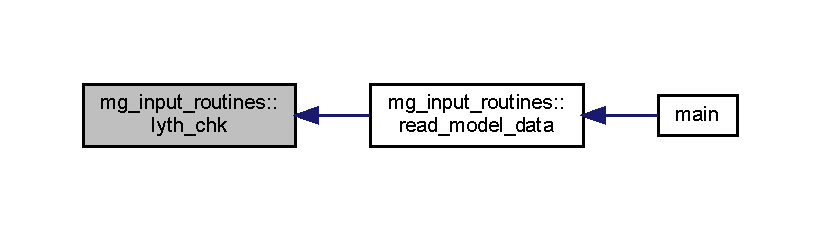
\includegraphics[width=350pt]{namespacemg__input__routines_a9e1339657e87110a735f9631657c9019_icgraph}
\end{center}
\end{figure}
\mbox{\Hypertarget{namespacemg__input__routines_acd1da063201ad2300b429047265d6c91}\label{namespacemg__input__routines_acd1da063201ad2300b429047265d6c91}} 
\index{mg\+\_\+input\+\_\+routines@{mg\+\_\+input\+\_\+routines}!read\+\_\+model\+\_\+data@{read\+\_\+model\+\_\+data}}
\index{read\+\_\+model\+\_\+data@{read\+\_\+model\+\_\+data}!mg\+\_\+input\+\_\+routines@{mg\+\_\+input\+\_\+routines}}
\subsubsection{\texorpdfstring{read\+\_\+model\+\_\+data()}{read\_model\_data()}}
{\footnotesize\ttfamily subroutine mg\+\_\+input\+\_\+routines\+::read\+\_\+model\+\_\+data (\begin{DoxyParamCaption}{ }\end{DoxyParamCaption})}

Here is the call graph for this function\+:
\nopagebreak
\begin{figure}[H]
\begin{center}
\leavevmode
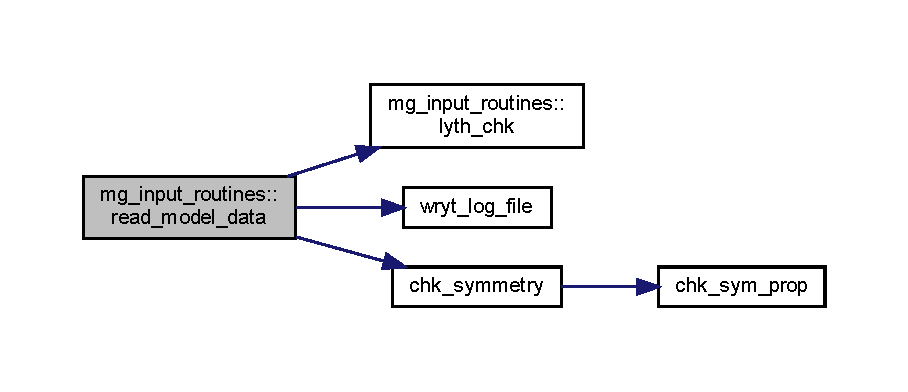
\includegraphics[width=350pt]{namespacemg__input__routines_acd1da063201ad2300b429047265d6c91_cgraph}
\end{center}
\end{figure}
Here is the caller graph for this function\+:
\nopagebreak
\begin{figure}[H]
\begin{center}
\leavevmode
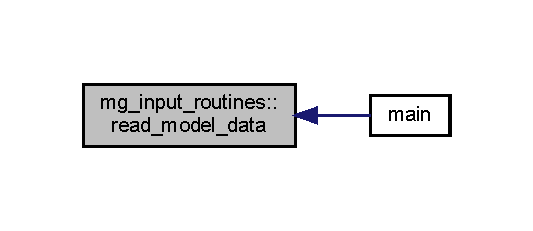
\includegraphics[width=256pt]{namespacemg__input__routines_acd1da063201ad2300b429047265d6c91_icgraph}
\end{center}
\end{figure}
\mbox{\Hypertarget{namespacemg__input__routines_a77a7419ce373edc9895839fc0d469d78}\label{namespacemg__input__routines_a77a7419ce373edc9895839fc0d469d78}} 
\index{mg\+\_\+input\+\_\+routines@{mg\+\_\+input\+\_\+routines}!read\+\_\+system\+\_\+data@{read\+\_\+system\+\_\+data}}
\index{read\+\_\+system\+\_\+data@{read\+\_\+system\+\_\+data}!mg\+\_\+input\+\_\+routines@{mg\+\_\+input\+\_\+routines}}
\subsubsection{\texorpdfstring{read\+\_\+system\+\_\+data()}{read\_system\_data()}}
{\footnotesize\ttfamily subroutine mg\+\_\+input\+\_\+routines\+::read\+\_\+system\+\_\+data (\begin{DoxyParamCaption}{ }\end{DoxyParamCaption})}

Here is the call graph for this function\+:
\nopagebreak
\begin{figure}[H]
\begin{center}
\leavevmode
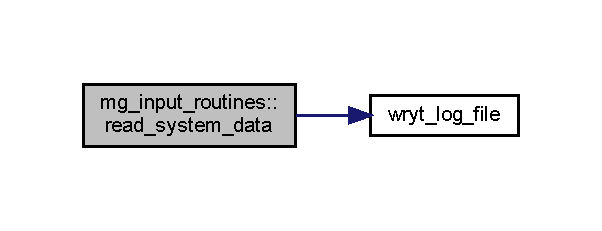
\includegraphics[width=289pt]{namespacemg__input__routines_a77a7419ce373edc9895839fc0d469d78_cgraph}
\end{center}
\end{figure}
Here is the caller graph for this function\+:
\nopagebreak
\begin{figure}[H]
\begin{center}
\leavevmode
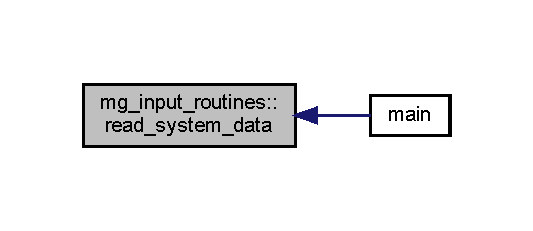
\includegraphics[width=256pt]{namespacemg__input__routines_a77a7419ce373edc9895839fc0d469d78_icgraph}
\end{center}
\end{figure}
\mbox{\Hypertarget{namespacemg__input__routines_ac8682ae293c93e95b72b4b7c222f9ed4}\label{namespacemg__input__routines_ac8682ae293c93e95b72b4b7c222f9ed4}} 
\index{mg\+\_\+input\+\_\+routines@{mg\+\_\+input\+\_\+routines}!set\+\_\+frq@{set\+\_\+frq}}
\index{set\+\_\+frq@{set\+\_\+frq}!mg\+\_\+input\+\_\+routines@{mg\+\_\+input\+\_\+routines}}
\subsubsection{\texorpdfstring{set\+\_\+frq()}{set\_frq()}}
{\footnotesize\ttfamily subroutine mg\+\_\+input\+\_\+routines\+::set\+\_\+frq (\begin{DoxyParamCaption}{ }\end{DoxyParamCaption})}

Here is the caller graph for this function\+:
\nopagebreak
\begin{figure}[H]
\begin{center}
\leavevmode
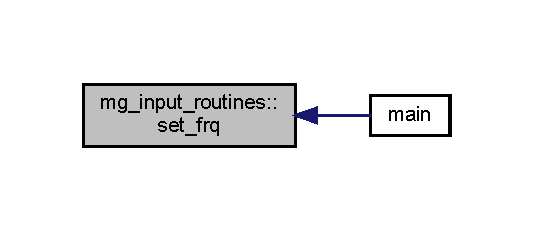
\includegraphics[width=256pt]{namespacemg__input__routines_ac8682ae293c93e95b72b4b7c222f9ed4_icgraph}
\end{center}
\end{figure}
\mbox{\Hypertarget{namespacemg__input__routines_af6f593fecea83164d8d0352ef801c23b}\label{namespacemg__input__routines_af6f593fecea83164d8d0352ef801c23b}} 
\index{mg\+\_\+input\+\_\+routines@{mg\+\_\+input\+\_\+routines}!set\+\_\+survey@{set\+\_\+survey}}
\index{set\+\_\+survey@{set\+\_\+survey}!mg\+\_\+input\+\_\+routines@{mg\+\_\+input\+\_\+routines}}
\subsubsection{\texorpdfstring{set\+\_\+survey()}{set\_survey()}}
{\footnotesize\ttfamily subroutine mg\+\_\+input\+\_\+routines\+::set\+\_\+survey (\begin{DoxyParamCaption}{ }\end{DoxyParamCaption})}

Here is the caller graph for this function\+:
\nopagebreak
\begin{figure}[H]
\begin{center}
\leavevmode
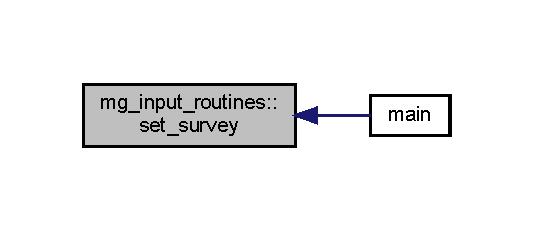
\includegraphics[width=256pt]{namespacemg__input__routines_af6f593fecea83164d8d0352ef801c23b_icgraph}
\end{center}
\end{figure}
\mbox{\Hypertarget{namespacemg__input__routines_a1b72deaf9809d0b370c1a68cd01e9d32}\label{namespacemg__input__routines_a1b72deaf9809d0b370c1a68cd01e9d32}} 
\index{mg\+\_\+input\+\_\+routines@{mg\+\_\+input\+\_\+routines}!set\+\_\+trp@{set\+\_\+trp}}
\index{set\+\_\+trp@{set\+\_\+trp}!mg\+\_\+input\+\_\+routines@{mg\+\_\+input\+\_\+routines}}
\subsubsection{\texorpdfstring{set\+\_\+trp()}{set\_trp()}}
{\footnotesize\ttfamily subroutine mg\+\_\+input\+\_\+routines\+::set\+\_\+trp (\begin{DoxyParamCaption}{ }\end{DoxyParamCaption})}

Here is the caller graph for this function\+:
\nopagebreak
\begin{figure}[H]
\begin{center}
\leavevmode
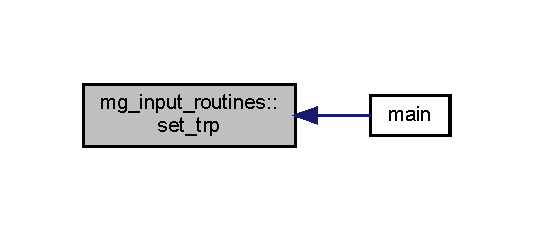
\includegraphics[width=256pt]{namespacemg__input__routines_a1b72deaf9809d0b370c1a68cd01e9d32_icgraph}
\end{center}
\end{figure}
\mbox{\Hypertarget{namespacemg__input__routines_a01c4f84680a9bc565592f441959beccc}\label{namespacemg__input__routines_a01c4f84680a9bc565592f441959beccc}} 
\index{mg\+\_\+input\+\_\+routines@{mg\+\_\+input\+\_\+routines}!show\+\_\+model@{show\+\_\+model}}
\index{show\+\_\+model@{show\+\_\+model}!mg\+\_\+input\+\_\+routines@{mg\+\_\+input\+\_\+routines}}
\subsubsection{\texorpdfstring{show\+\_\+model()}{show\_model()}}
{\footnotesize\ttfamily subroutine mg\+\_\+input\+\_\+routines\+::show\+\_\+model (\begin{DoxyParamCaption}{ }\end{DoxyParamCaption})}

Here is the caller graph for this function\+:
\nopagebreak
\begin{figure}[H]
\begin{center}
\leavevmode
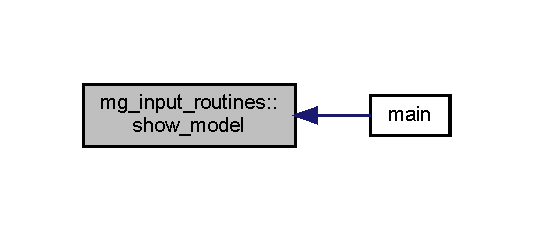
\includegraphics[width=256pt]{namespacemg__input__routines_a01c4f84680a9bc565592f441959beccc_icgraph}
\end{center}
\end{figure}


\subsection{Variable Documentation}
\mbox{\Hypertarget{namespacemg__input__routines_a028ce31030b8cbaac07934598f1bb0b3}\label{namespacemg__input__routines_a028ce31030b8cbaac07934598f1bb0b3}} 
\index{mg\+\_\+input\+\_\+routines@{mg\+\_\+input\+\_\+routines}!bhaz@{bhaz}}
\index{bhaz@{bhaz}!mg\+\_\+input\+\_\+routines@{mg\+\_\+input\+\_\+routines}}
\subsubsection{\texorpdfstring{bhaz}{bhaz}}
{\footnotesize\ttfamily real, dimension(\+:,\+:), allocatable mg\+\_\+input\+\_\+routines\+::bhaz}

\mbox{\Hypertarget{namespacemg__input__routines_a2cf5a853bfa353bf9d25a57b6aac283a}\label{namespacemg__input__routines_a2cf5a853bfa353bf9d25a57b6aac283a}} 
\index{mg\+\_\+input\+\_\+routines@{mg\+\_\+input\+\_\+routines}!bhdip@{bhdip}}
\index{bhdip@{bhdip}!mg\+\_\+input\+\_\+routines@{mg\+\_\+input\+\_\+routines}}
\subsubsection{\texorpdfstring{bhdip}{bhdip}}
{\footnotesize\ttfamily real, dimension(\+:,\+:), allocatable mg\+\_\+input\+\_\+routines\+::bhdip}

\mbox{\Hypertarget{namespacemg__input__routines_ab21b53ae17d7a35ba5def7f4466da62d}\label{namespacemg__input__routines_ab21b53ae17d7a35ba5def7f4466da62d}} 
\index{mg\+\_\+input\+\_\+routines@{mg\+\_\+input\+\_\+routines}!bhr@{bhr}}
\index{bhr@{bhr}!mg\+\_\+input\+\_\+routines@{mg\+\_\+input\+\_\+routines}}
\subsubsection{\texorpdfstring{bhr}{bhr}}
{\footnotesize\ttfamily logical, dimension(\+:,\+:), allocatable mg\+\_\+input\+\_\+routines\+::bhr}

\mbox{\Hypertarget{namespacemg__input__routines_a942bb74999b46c3142791ee0bc5420a0}\label{namespacemg__input__routines_a942bb74999b46c3142791ee0bc5420a0}} 
\index{mg\+\_\+input\+\_\+routines@{mg\+\_\+input\+\_\+routines}!cfreq@{cfreq}}
\index{cfreq@{cfreq}!mg\+\_\+input\+\_\+routines@{mg\+\_\+input\+\_\+routines}}
\subsubsection{\texorpdfstring{cfreq}{cfreq}}
{\footnotesize\ttfamily real, dimension(\+:), allocatable mg\+\_\+input\+\_\+routines\+::cfreq}

\mbox{\Hypertarget{namespacemg__input__routines_a45b54b5e8dc7da41f04656a21595105c}\label{namespacemg__input__routines_a45b54b5e8dc7da41f04656a21595105c}} 
\index{mg\+\_\+input\+\_\+routines@{mg\+\_\+input\+\_\+routines}!chrg@{chrg}}
\index{chrg@{chrg}!mg\+\_\+input\+\_\+routines@{mg\+\_\+input\+\_\+routines}}
\subsubsection{\texorpdfstring{chrg}{chrg}}
{\footnotesize\ttfamily real, dimension(\+:), allocatable mg\+\_\+input\+\_\+routines\+::chrg}

\mbox{\Hypertarget{namespacemg__input__routines_a3f4fc21cf71d14b405a57f9ede298ded}\label{namespacemg__input__routines_a3f4fc21cf71d14b405a57f9ede298ded}} 
\index{mg\+\_\+input\+\_\+routines@{mg\+\_\+input\+\_\+routines}!clcd@{clcd}}
\index{clcd@{clcd}!mg\+\_\+input\+\_\+routines@{mg\+\_\+input\+\_\+routines}}
\subsubsection{\texorpdfstring{clcd}{clcd}}
{\footnotesize\ttfamily real(kind=8), dimension(\+:,\+:), allocatable mg\+\_\+input\+\_\+routines\+::clcd}

\mbox{\Hypertarget{namespacemg__input__routines_aff413a8a8457c1b1ae4dc95fa3929e22}\label{namespacemg__input__routines_aff413a8a8457c1b1ae4dc95fa3929e22}} 
\index{mg\+\_\+input\+\_\+routines@{mg\+\_\+input\+\_\+routines}!cmp@{cmp}}
\index{cmp@{cmp}!mg\+\_\+input\+\_\+routines@{mg\+\_\+input\+\_\+routines}}
\subsubsection{\texorpdfstring{cmp}{cmp}}
{\footnotesize\ttfamily integer, dimension(\+:), allocatable mg\+\_\+input\+\_\+routines\+::cmp}

\mbox{\Hypertarget{namespacemg__input__routines_a677ccea5b7c4699e0d7c0620fb4473c7}\label{namespacemg__input__routines_a677ccea5b7c4699e0d7c0620fb4473c7}} 
\index{mg\+\_\+input\+\_\+routines@{mg\+\_\+input\+\_\+routines}!ctau@{ctau}}
\index{ctau@{ctau}!mg\+\_\+input\+\_\+routines@{mg\+\_\+input\+\_\+routines}}
\subsubsection{\texorpdfstring{ctau}{ctau}}
{\footnotesize\ttfamily real, dimension(\+:), allocatable mg\+\_\+input\+\_\+routines\+::ctau}

\mbox{\Hypertarget{namespacemg__input__routines_ad16e03a98826653c76c46073ce55bf5c}\label{namespacemg__input__routines_ad16e03a98826653c76c46073ce55bf5c}} 
\index{mg\+\_\+input\+\_\+routines@{mg\+\_\+input\+\_\+routines}!curnt@{curnt}}
\index{curnt@{curnt}!mg\+\_\+input\+\_\+routines@{mg\+\_\+input\+\_\+routines}}
\subsubsection{\texorpdfstring{curnt}{curnt}}
{\footnotesize\ttfamily real, dimension(\+:), allocatable mg\+\_\+input\+\_\+routines\+::curnt}

\mbox{\Hypertarget{namespacemg__input__routines_abccc4c4d25850b657fcca7f97c1e6059}\label{namespacemg__input__routines_abccc4c4d25850b657fcca7f97c1e6059}} 
\index{mg\+\_\+input\+\_\+routines@{mg\+\_\+input\+\_\+routines}!do3d@{do3d}}
\index{do3d@{do3d}!mg\+\_\+input\+\_\+routines@{mg\+\_\+input\+\_\+routines}}
\subsubsection{\texorpdfstring{do3d}{do3d}}
{\footnotesize\ttfamily integer mg\+\_\+input\+\_\+routines\+::do3d}

\mbox{\Hypertarget{namespacemg__input__routines_aa1f05f7245fd87ee0872f3d87b6f5711}\label{namespacemg__input__routines_aa1f05f7245fd87ee0872f3d87b6f5711}} 
\index{mg\+\_\+input\+\_\+routines@{mg\+\_\+input\+\_\+routines}!ecntrd@{ecntrd}}
\index{ecntrd@{ecntrd}!mg\+\_\+input\+\_\+routines@{mg\+\_\+input\+\_\+routines}}
\subsubsection{\texorpdfstring{ecntrd}{ecntrd}}
{\footnotesize\ttfamily real(kind=8) mg\+\_\+input\+\_\+routines\+::ecntrd}

\mbox{\Hypertarget{namespacemg__input__routines_aed0c04ce17d1cbf624d2544819459544}\label{namespacemg__input__routines_aed0c04ce17d1cbf624d2544819459544}} 
\index{mg\+\_\+input\+\_\+routines@{mg\+\_\+input\+\_\+routines}!freq@{freq}}
\index{freq@{freq}!mg\+\_\+input\+\_\+routines@{mg\+\_\+input\+\_\+routines}}
\subsubsection{\texorpdfstring{freq}{freq}}
{\footnotesize\ttfamily real, dimension(\+:), allocatable mg\+\_\+input\+\_\+routines\+::freq}

\mbox{\Hypertarget{namespacemg__input__routines_a11bf44e1f047050fb335bf4bfc8d1a2c}\label{namespacemg__input__routines_a11bf44e1f047050fb335bf4bfc8d1a2c}} 
\index{mg\+\_\+input\+\_\+routines@{mg\+\_\+input\+\_\+routines}!gnd\+\_\+lvl@{gnd\+\_\+lvl}}
\index{gnd\+\_\+lvl@{gnd\+\_\+lvl}!mg\+\_\+input\+\_\+routines@{mg\+\_\+input\+\_\+routines}}
\subsubsection{\texorpdfstring{gnd\+\_\+lvl}{gnd\_lvl}}
{\footnotesize\ttfamily real mg\+\_\+input\+\_\+routines\+::gnd\+\_\+lvl}

\mbox{\Hypertarget{namespacemg__input__routines_a32db71951a8a9e2fd94dd117598cdeb6}\label{namespacemg__input__routines_a32db71951a8a9e2fd94dd117598cdeb6}} 
\index{mg\+\_\+input\+\_\+routines@{mg\+\_\+input\+\_\+routines}!id\+\_\+lith@{id\+\_\+lith}}
\index{id\+\_\+lith@{id\+\_\+lith}!mg\+\_\+input\+\_\+routines@{mg\+\_\+input\+\_\+routines}}
\subsubsection{\texorpdfstring{id\+\_\+lith}{id\_lith}}
{\footnotesize\ttfamily integer, dimension(\+:), allocatable mg\+\_\+input\+\_\+routines\+::id\+\_\+lith}

\mbox{\Hypertarget{namespacemg__input__routines_a8e5e63f1a08c24f363056fa6ddf7b302}\label{namespacemg__input__routines_a8e5e63f1a08c24f363056fa6ddf7b302}} 
\index{mg\+\_\+input\+\_\+routines@{mg\+\_\+input\+\_\+routines}!inp@{inp}}
\index{inp@{inp}!mg\+\_\+input\+\_\+routines@{mg\+\_\+input\+\_\+routines}}
\subsubsection{\texorpdfstring{inp}{inp}}
{\footnotesize\ttfamily character (len=120) mg\+\_\+input\+\_\+routines\+::inp}

\mbox{\Hypertarget{namespacemg__input__routines_a7d3adc6f4d1d09319400a6a90b644ccf}\label{namespacemg__input__routines_a7d3adc6f4d1d09319400a6a90b644ccf}} 
\index{mg\+\_\+input\+\_\+routines@{mg\+\_\+input\+\_\+routines}!istop@{istop}}
\index{istop@{istop}!mg\+\_\+input\+\_\+routines@{mg\+\_\+input\+\_\+routines}}
\subsubsection{\texorpdfstring{istop}{istop}}
{\footnotesize\ttfamily integer mg\+\_\+input\+\_\+routines\+::istop}

\mbox{\Hypertarget{namespacemg__input__routines_a292a26be6620117a94388a4961626b88}\label{namespacemg__input__routines_a292a26be6620117a94388a4961626b88}} 
\index{mg\+\_\+input\+\_\+routines@{mg\+\_\+input\+\_\+routines}!j@{j}}
\index{j@{j}!mg\+\_\+input\+\_\+routines@{mg\+\_\+input\+\_\+routines}}
\subsubsection{\texorpdfstring{j}{j}}
{\footnotesize\ttfamily integer mg\+\_\+input\+\_\+routines\+::j}

\mbox{\Hypertarget{namespacemg__input__routines_ad6477edd6c31520d925c6962ec2a7248}\label{namespacemg__input__routines_ad6477edd6c31520d925c6962ec2a7248}} 
\index{mg\+\_\+input\+\_\+routines@{mg\+\_\+input\+\_\+routines}!jb@{jb}}
\index{jb@{jb}!mg\+\_\+input\+\_\+routines@{mg\+\_\+input\+\_\+routines}}
\subsubsection{\texorpdfstring{jb}{jb}}
{\footnotesize\ttfamily integer mg\+\_\+input\+\_\+routines\+::jb}

\mbox{\Hypertarget{namespacemg__input__routines_aa46cdfb9e05dba796c09d3b429b4b570}\label{namespacemg__input__routines_aa46cdfb9e05dba796c09d3b429b4b570}} 
\index{mg\+\_\+input\+\_\+routines@{mg\+\_\+input\+\_\+routines}!jg@{jg}}
\index{jg@{jg}!mg\+\_\+input\+\_\+routines@{mg\+\_\+input\+\_\+routines}}
\subsubsection{\texorpdfstring{jg}{jg}}
{\footnotesize\ttfamily integer mg\+\_\+input\+\_\+routines\+::jg}

\mbox{\Hypertarget{namespacemg__input__routines_ac9c41f20a75b4f15a95c79ffcbf655db}\label{namespacemg__input__routines_ac9c41f20a75b4f15a95c79ffcbf655db}} 
\index{mg\+\_\+input\+\_\+routines@{mg\+\_\+input\+\_\+routines}!jl@{jl}}
\index{jl@{jl}!mg\+\_\+input\+\_\+routines@{mg\+\_\+input\+\_\+routines}}
\subsubsection{\texorpdfstring{jl}{jl}}
{\footnotesize\ttfamily integer mg\+\_\+input\+\_\+routines\+::jl}

\mbox{\Hypertarget{namespacemg__input__routines_a03f300f92ef7ffa2899bc4a7623805e6}\label{namespacemg__input__routines_a03f300f92ef7ffa2899bc4a7623805e6}} 
\index{mg\+\_\+input\+\_\+routines@{mg\+\_\+input\+\_\+routines}!jp@{jp}}
\index{jp@{jp}!mg\+\_\+input\+\_\+routines@{mg\+\_\+input\+\_\+routines}}
\subsubsection{\texorpdfstring{jp}{jp}}
{\footnotesize\ttfamily integer mg\+\_\+input\+\_\+routines\+::jp}

\mbox{\Hypertarget{namespacemg__input__routines_a904a6771d079976761e82cd541845078}\label{namespacemg__input__routines_a904a6771d079976761e82cd541845078}} 
\index{mg\+\_\+input\+\_\+routines@{mg\+\_\+input\+\_\+routines}!jr@{jr}}
\index{jr@{jr}!mg\+\_\+input\+\_\+routines@{mg\+\_\+input\+\_\+routines}}
\subsubsection{\texorpdfstring{jr}{jr}}
{\footnotesize\ttfamily integer mg\+\_\+input\+\_\+routines\+::jr}

\mbox{\Hypertarget{namespacemg__input__routines_a2ac0c5af92f879279450a35f8f6f407d}\label{namespacemg__input__routines_a2ac0c5af92f879279450a35f8f6f407d}} 
\index{mg\+\_\+input\+\_\+routines@{mg\+\_\+input\+\_\+routines}!js@{js}}
\index{js@{js}!mg\+\_\+input\+\_\+routines@{mg\+\_\+input\+\_\+routines}}
\subsubsection{\texorpdfstring{js}{js}}
{\footnotesize\ttfamily integer mg\+\_\+input\+\_\+routines\+::js}

\mbox{\Hypertarget{namespacemg__input__routines_a7f93d05f71f46f0de859cdfc4627cf47}\label{namespacemg__input__routines_a7f93d05f71f46f0de859cdfc4627cf47}} 
\index{mg\+\_\+input\+\_\+routines@{mg\+\_\+input\+\_\+routines}!jt@{jt}}
\index{jt@{jt}!mg\+\_\+input\+\_\+routines@{mg\+\_\+input\+\_\+routines}}
\subsubsection{\texorpdfstring{jt}{jt}}
{\footnotesize\ttfamily integer mg\+\_\+input\+\_\+routines\+::jt}

\mbox{\Hypertarget{namespacemg__input__routines_a9e46f68f8402c238d9dc7938d1c1a333}\label{namespacemg__input__routines_a9e46f68f8402c238d9dc7938d1c1a333}} 
\index{mg\+\_\+input\+\_\+routines@{mg\+\_\+input\+\_\+routines}!jv@{jv}}
\index{jv@{jv}!mg\+\_\+input\+\_\+routines@{mg\+\_\+input\+\_\+routines}}
\subsubsection{\texorpdfstring{jv}{jv}}
{\footnotesize\ttfamily integer mg\+\_\+input\+\_\+routines\+::jv}

\mbox{\Hypertarget{namespacemg__input__routines_ad19c4bbecbed200a723fcb0cba57fb56}\label{namespacemg__input__routines_ad19c4bbecbed200a723fcb0cba57fb56}} 
\index{mg\+\_\+input\+\_\+routines@{mg\+\_\+input\+\_\+routines}!kacc@{kacc}}
\index{kacc@{kacc}!mg\+\_\+input\+\_\+routines@{mg\+\_\+input\+\_\+routines}}
\subsubsection{\texorpdfstring{kacc}{kacc}}
{\footnotesize\ttfamily integer mg\+\_\+input\+\_\+routines\+::kacc}

\mbox{\Hypertarget{namespacemg__input__routines_a7d0a5bd49c58f7353a16d46811fa6fb0}\label{namespacemg__input__routines_a7d0a5bd49c58f7353a16d46811fa6fb0}} 
\index{mg\+\_\+input\+\_\+routines@{mg\+\_\+input\+\_\+routines}!kfrqe@{kfrqe}}
\index{kfrqe@{kfrqe}!mg\+\_\+input\+\_\+routines@{mg\+\_\+input\+\_\+routines}}
\subsubsection{\texorpdfstring{kfrqe}{kfrqe}}
{\footnotesize\ttfamily integer mg\+\_\+input\+\_\+routines\+::kfrqe}

\mbox{\Hypertarget{namespacemg__input__routines_a689c313caea9666b0564a35579678ce1}\label{namespacemg__input__routines_a689c313caea9666b0564a35579678ce1}} 
\index{mg\+\_\+input\+\_\+routines@{mg\+\_\+input\+\_\+routines}!krxw@{krxw}}
\index{krxw@{krxw}!mg\+\_\+input\+\_\+routines@{mg\+\_\+input\+\_\+routines}}
\subsubsection{\texorpdfstring{krxw}{krxw}}
{\footnotesize\ttfamily integer mg\+\_\+input\+\_\+routines\+::krxw}

\mbox{\Hypertarget{namespacemg__input__routines_ad66a5f5acff5c1b06da85bb8a46384cd}\label{namespacemg__input__routines_ad66a5f5acff5c1b06da85bb8a46384cd}} 
\index{mg\+\_\+input\+\_\+routines@{mg\+\_\+input\+\_\+routines}!ksymm@{ksymm}}
\index{ksymm@{ksymm}!mg\+\_\+input\+\_\+routines@{mg\+\_\+input\+\_\+routines}}
\subsubsection{\texorpdfstring{ksymm}{ksymm}}
{\footnotesize\ttfamily integer mg\+\_\+input\+\_\+routines\+::ksymm}

\mbox{\Hypertarget{namespacemg__input__routines_a5bfda764a44cea47087fc53cd4d756d0}\label{namespacemg__input__routines_a5bfda764a44cea47087fc53cd4d756d0}} 
\index{mg\+\_\+input\+\_\+routines@{mg\+\_\+input\+\_\+routines}!lithl@{lithl}}
\index{lithl@{lithl}!mg\+\_\+input\+\_\+routines@{mg\+\_\+input\+\_\+routines}}
\subsubsection{\texorpdfstring{lithl}{lithl}}
{\footnotesize\ttfamily integer, dimension(\+:), allocatable mg\+\_\+input\+\_\+routines\+::lithl}

\mbox{\Hypertarget{namespacemg__input__routines_ace92ffb4ec110b849313b8e1fdc6893a}\label{namespacemg__input__routines_ace92ffb4ec110b849313b8e1fdc6893a}} 
\index{mg\+\_\+input\+\_\+routines@{mg\+\_\+input\+\_\+routines}!lithp@{lithp}}
\index{lithp@{lithp}!mg\+\_\+input\+\_\+routines@{mg\+\_\+input\+\_\+routines}}
\subsubsection{\texorpdfstring{lithp}{lithp}}
{\footnotesize\ttfamily real, dimension(\+:), allocatable mg\+\_\+input\+\_\+routines\+::lithp}

\mbox{\Hypertarget{namespacemg__input__routines_aeea0329fda5c5a9795228e5b810aadbf}\label{namespacemg__input__routines_aeea0329fda5c5a9795228e5b810aadbf}} 
\index{mg\+\_\+input\+\_\+routines@{mg\+\_\+input\+\_\+routines}!lrx@{lrx}}
\index{lrx@{lrx}!mg\+\_\+input\+\_\+routines@{mg\+\_\+input\+\_\+routines}}
\subsubsection{\texorpdfstring{lrx}{lrx}}
{\footnotesize\ttfamily integer mg\+\_\+input\+\_\+routines\+::lrx}

\mbox{\Hypertarget{namespacemg__input__routines_aa9693c554c4256fdbbe5ed5a0bc7976f}\label{namespacemg__input__routines_aa9693c554c4256fdbbe5ed5a0bc7976f}} 
\index{mg\+\_\+input\+\_\+routines@{mg\+\_\+input\+\_\+routines}!lyth@{lyth}}
\index{lyth@{lyth}!mg\+\_\+input\+\_\+routines@{mg\+\_\+input\+\_\+routines}}
\subsubsection{\texorpdfstring{lyth}{lyth}}
{\footnotesize\ttfamily real, dimension(\+:,\+:), allocatable mg\+\_\+input\+\_\+routines\+::lyth}

\mbox{\Hypertarget{namespacemg__input__routines_a9c6fc602bbc9b8c29310af346d80ad74}\label{namespacemg__input__routines_a9c6fc602bbc9b8c29310af346d80ad74}} 
\index{mg\+\_\+input\+\_\+routines@{mg\+\_\+input\+\_\+routines}!maxfrq@{maxfrq}}
\index{maxfrq@{maxfrq}!mg\+\_\+input\+\_\+routines@{mg\+\_\+input\+\_\+routines}}
\subsubsection{\texorpdfstring{maxfrq}{maxfrq}}
{\footnotesize\ttfamily real mg\+\_\+input\+\_\+routines\+::maxfrq}

\mbox{\Hypertarget{namespacemg__input__routines_a0c365e2dbdbd75369df81405c3e5667f}\label{namespacemg__input__routines_a0c365e2dbdbd75369df81405c3e5667f}} 
\index{mg\+\_\+input\+\_\+routines@{mg\+\_\+input\+\_\+routines}!minfrq@{minfrq}}
\index{minfrq@{minfrq}!mg\+\_\+input\+\_\+routines@{mg\+\_\+input\+\_\+routines}}
\subsubsection{\texorpdfstring{minfrq}{minfrq}}
{\footnotesize\ttfamily real mg\+\_\+input\+\_\+routines\+::minfrq}

\mbox{\Hypertarget{namespacemg__input__routines_a67aa10eca6fcaa9b0bb58f754f9601e4}\label{namespacemg__input__routines_a67aa10eca6fcaa9b0bb58f754f9601e4}} 
\index{mg\+\_\+input\+\_\+routines@{mg\+\_\+input\+\_\+routines}!mqvr@{mqvr}}
\index{mqvr@{mqvr}!mg\+\_\+input\+\_\+routines@{mg\+\_\+input\+\_\+routines}}
\subsubsection{\texorpdfstring{mqvr}{mqvr}}
{\footnotesize\ttfamily integer mg\+\_\+input\+\_\+routines\+::mqvr}

\mbox{\Hypertarget{namespacemg__input__routines_a7d8e6d20b2ea422eec9c2aa426127bb1}\label{namespacemg__input__routines_a7d8e6d20b2ea422eec9c2aa426127bb1}} 
\index{mg\+\_\+input\+\_\+routines@{mg\+\_\+input\+\_\+routines}!mrx@{mrx}}
\index{mrx@{mrx}!mg\+\_\+input\+\_\+routines@{mg\+\_\+input\+\_\+routines}}
\subsubsection{\texorpdfstring{mrx}{mrx}}
{\footnotesize\ttfamily integer mg\+\_\+input\+\_\+routines\+::mrx}

\mbox{\Hypertarget{namespacemg__input__routines_a6485fb3eba9b87bb80aaac69bb342695}\label{namespacemg__input__routines_a6485fb3eba9b87bb80aaac69bb342695}} 
\index{mg\+\_\+input\+\_\+routines@{mg\+\_\+input\+\_\+routines}!msg@{msg}}
\index{msg@{msg}!mg\+\_\+input\+\_\+routines@{mg\+\_\+input\+\_\+routines}}
\subsubsection{\texorpdfstring{msg}{msg}}
{\footnotesize\ttfamily integer mg\+\_\+input\+\_\+routines\+::msg}

\mbox{\Hypertarget{namespacemg__input__routines_a079d18c936f009ac6113cc598db36422}\label{namespacemg__input__routines_a079d18c936f009ac6113cc598db36422}} 
\index{mg\+\_\+input\+\_\+routines@{mg\+\_\+input\+\_\+routines}!mxerr@{mxerr}}
\index{mxerr@{mxerr}!mg\+\_\+input\+\_\+routines@{mg\+\_\+input\+\_\+routines}}
\subsubsection{\texorpdfstring{mxerr}{mxerr}}
{\footnotesize\ttfamily integer mg\+\_\+input\+\_\+routines\+::mxerr}

\mbox{\Hypertarget{namespacemg__input__routines_a0af8fff8410098941c2a2c06279fad18}\label{namespacemg__input__routines_a0af8fff8410098941c2a2c06279fad18}} 
\index{mg\+\_\+input\+\_\+routines@{mg\+\_\+input\+\_\+routines}!mxfrqe@{mxfrqe}}
\index{mxfrqe@{mxfrqe}!mg\+\_\+input\+\_\+routines@{mg\+\_\+input\+\_\+routines}}
\subsubsection{\texorpdfstring{mxfrqe}{mxfrqe}}
{\footnotesize\ttfamily real mg\+\_\+input\+\_\+routines\+::mxfrqe}

\mbox{\Hypertarget{namespacemg__input__routines_ad7f27d4e899695dc12c5b45ea797b177}\label{namespacemg__input__routines_ad7f27d4e899695dc12c5b45ea797b177}} 
\index{mg\+\_\+input\+\_\+routines@{mg\+\_\+input\+\_\+routines}!mxvrtx@{mxvrtx}}
\index{mxvrtx@{mxvrtx}!mg\+\_\+input\+\_\+routines@{mg\+\_\+input\+\_\+routines}}
\subsubsection{\texorpdfstring{mxvrtx}{mxvrtx}}
{\footnotesize\ttfamily integer mg\+\_\+input\+\_\+routines\+::mxvrtx}

\mbox{\Hypertarget{namespacemg__input__routines_a4c570440af762e32ddd4471fd251db81}\label{namespacemg__input__routines_a4c570440af762e32ddd4471fd251db81}} 
\index{mg\+\_\+input\+\_\+routines@{mg\+\_\+input\+\_\+routines}!n\+\_\+vrtx@{n\+\_\+vrtx}}
\index{n\+\_\+vrtx@{n\+\_\+vrtx}!mg\+\_\+input\+\_\+routines@{mg\+\_\+input\+\_\+routines}}
\subsubsection{\texorpdfstring{n\+\_\+vrtx}{n\_vrtx}}
{\footnotesize\ttfamily integer, dimension(\+:), allocatable mg\+\_\+input\+\_\+routines\+::n\+\_\+vrtx}

\mbox{\Hypertarget{namespacemg__input__routines_ac7e71234c4ec9ad59fd8b0d33c8809af}\label{namespacemg__input__routines_ac7e71234c4ec9ad59fd8b0d33c8809af}} 
\index{mg\+\_\+input\+\_\+routines@{mg\+\_\+input\+\_\+routines}!ncell\+\_\+ew@{ncell\+\_\+ew}}
\index{ncell\+\_\+ew@{ncell\+\_\+ew}!mg\+\_\+input\+\_\+routines@{mg\+\_\+input\+\_\+routines}}
\subsubsection{\texorpdfstring{ncell\+\_\+ew}{ncell\_ew}}
{\footnotesize\ttfamily integer, dimension (\+:), allocatable mg\+\_\+input\+\_\+routines\+::ncell\+\_\+ew}

\mbox{\Hypertarget{namespacemg__input__routines_aec49c121aaee899e4b0f33bf6943bcb4}\label{namespacemg__input__routines_aec49c121aaee899e4b0f33bf6943bcb4}} 
\index{mg\+\_\+input\+\_\+routines@{mg\+\_\+input\+\_\+routines}!ncell\+\_\+ns@{ncell\+\_\+ns}}
\index{ncell\+\_\+ns@{ncell\+\_\+ns}!mg\+\_\+input\+\_\+routines@{mg\+\_\+input\+\_\+routines}}
\subsubsection{\texorpdfstring{ncell\+\_\+ns}{ncell\_ns}}
{\footnotesize\ttfamily integer, dimension (\+:), allocatable mg\+\_\+input\+\_\+routines\+::ncell\+\_\+ns}

\mbox{\Hypertarget{namespacemg__input__routines_a0a0ce37b6540f74233bf3aadaa260f96}\label{namespacemg__input__routines_a0a0ce37b6540f74233bf3aadaa260f96}} 
\index{mg\+\_\+input\+\_\+routines@{mg\+\_\+input\+\_\+routines}!ncell\+\_\+z@{ncell\+\_\+z}}
\index{ncell\+\_\+z@{ncell\+\_\+z}!mg\+\_\+input\+\_\+routines@{mg\+\_\+input\+\_\+routines}}
\subsubsection{\texorpdfstring{ncell\+\_\+z}{ncell\_z}}
{\footnotesize\ttfamily integer, dimension (\+:), allocatable mg\+\_\+input\+\_\+routines\+::ncell\+\_\+z}

\mbox{\Hypertarget{namespacemg__input__routines_a29d81574f8ee97737139da90c94a3614}\label{namespacemg__input__routines_a29d81574f8ee97737139da90c94a3614}} 
\index{mg\+\_\+input\+\_\+routines@{mg\+\_\+input\+\_\+routines}!nchnl@{nchnl}}
\index{nchnl@{nchnl}!mg\+\_\+input\+\_\+routines@{mg\+\_\+input\+\_\+routines}}
\subsubsection{\texorpdfstring{nchnl}{nchnl}}
{\footnotesize\ttfamily integer mg\+\_\+input\+\_\+routines\+::nchnl}

\mbox{\Hypertarget{namespacemg__input__routines_a22d278bfaca850a0ab774373e78661ec}\label{namespacemg__input__routines_a22d278bfaca850a0ab774373e78661ec}} 
\index{mg\+\_\+input\+\_\+routines@{mg\+\_\+input\+\_\+routines}!ncmp@{ncmp}}
\index{ncmp@{ncmp}!mg\+\_\+input\+\_\+routines@{mg\+\_\+input\+\_\+routines}}
\subsubsection{\texorpdfstring{ncmp}{ncmp}}
{\footnotesize\ttfamily integer, dimension(\+:,\+:), allocatable mg\+\_\+input\+\_\+routines\+::ncmp}

\mbox{\Hypertarget{namespacemg__input__routines_ab931c6d3ad288e3913d59d1b5352da79}\label{namespacemg__input__routines_ab931c6d3ad288e3913d59d1b5352da79}} 
\index{mg\+\_\+input\+\_\+routines@{mg\+\_\+input\+\_\+routines}!ncmpg@{ncmpg}}
\index{ncmpg@{ncmpg}!mg\+\_\+input\+\_\+routines@{mg\+\_\+input\+\_\+routines}}
\subsubsection{\texorpdfstring{ncmpg}{ncmpg}}
{\footnotesize\ttfamily integer, dimension(\+:), allocatable mg\+\_\+input\+\_\+routines\+::ncmpg}

\mbox{\Hypertarget{namespacemg__input__routines_a7a7ebfe0ae5724156d7e5a4bc92d1b7a}\label{namespacemg__input__routines_a7a7ebfe0ae5724156d7e5a4bc92d1b7a}} 
\index{mg\+\_\+input\+\_\+routines@{mg\+\_\+input\+\_\+routines}!ncntrd@{ncntrd}}
\index{ncntrd@{ncntrd}!mg\+\_\+input\+\_\+routines@{mg\+\_\+input\+\_\+routines}}
\subsubsection{\texorpdfstring{ncntrd}{ncntrd}}
{\footnotesize\ttfamily real(kind=8) mg\+\_\+input\+\_\+routines\+::ncntrd}

\mbox{\Hypertarget{namespacemg__input__routines_a310ddcda277a3a2743d7709cccdf9007}\label{namespacemg__input__routines_a310ddcda277a3a2743d7709cccdf9007}} 
\index{mg\+\_\+input\+\_\+routines@{mg\+\_\+input\+\_\+routines}!nd@{nd}}
\index{nd@{nd}!mg\+\_\+input\+\_\+routines@{mg\+\_\+input\+\_\+routines}}
\subsubsection{\texorpdfstring{nd}{nd}}
{\footnotesize\ttfamily integer mg\+\_\+input\+\_\+routines\+::nd}

\mbox{\Hypertarget{namespacemg__input__routines_a494cce161b67dc2a3a628e7ce33d35d0}\label{namespacemg__input__routines_a494cce161b67dc2a3a628e7ce33d35d0}} 
\index{mg\+\_\+input\+\_\+routines@{mg\+\_\+input\+\_\+routines}!ndr@{ndr}}
\index{ndr@{ndr}!mg\+\_\+input\+\_\+routines@{mg\+\_\+input\+\_\+routines}}
\subsubsection{\texorpdfstring{ndr}{ndr}}
{\footnotesize\ttfamily integer mg\+\_\+input\+\_\+routines\+::ndr}

\mbox{\Hypertarget{namespacemg__input__routines_aed1d27aadf7cdaefb4565f0ef803464d}\label{namespacemg__input__routines_aed1d27aadf7cdaefb4565f0ef803464d}} 
\index{mg\+\_\+input\+\_\+routines@{mg\+\_\+input\+\_\+routines}!nevents@{nevents}}
\index{nevents@{nevents}!mg\+\_\+input\+\_\+routines@{mg\+\_\+input\+\_\+routines}}
\subsubsection{\texorpdfstring{nevents}{nevents}}
{\footnotesize\ttfamily integer mg\+\_\+input\+\_\+routines\+::nevents}

\mbox{\Hypertarget{namespacemg__input__routines_a733484f25916ecd427704c6769db1ba1}\label{namespacemg__input__routines_a733484f25916ecd427704c6769db1ba1}} 
\index{mg\+\_\+input\+\_\+routines@{mg\+\_\+input\+\_\+routines}!new@{new}}
\index{new@{new}!mg\+\_\+input\+\_\+routines@{mg\+\_\+input\+\_\+routines}}
\subsubsection{\texorpdfstring{new}{new}}
{\footnotesize\ttfamily logical mg\+\_\+input\+\_\+routines\+::new}

\mbox{\Hypertarget{namespacemg__input__routines_ae01275ae75f29d76acacfc4e14d6ec15}\label{namespacemg__input__routines_ae01275ae75f29d76acacfc4e14d6ec15}} 
\index{mg\+\_\+input\+\_\+routines@{mg\+\_\+input\+\_\+routines}!nfrq@{nfrq}}
\index{nfrq@{nfrq}!mg\+\_\+input\+\_\+routines@{mg\+\_\+input\+\_\+routines}}
\subsubsection{\texorpdfstring{nfrq}{nfrq}}
{\footnotesize\ttfamily integer mg\+\_\+input\+\_\+routines\+::nfrq}

\mbox{\Hypertarget{namespacemg__input__routines_a02fb693b7d09302d47008f0a381ea329}\label{namespacemg__input__routines_a02fb693b7d09302d47008f0a381ea329}} 
\index{mg\+\_\+input\+\_\+routines@{mg\+\_\+input\+\_\+routines}!nlg@{nlg}}
\index{nlg@{nlg}!mg\+\_\+input\+\_\+routines@{mg\+\_\+input\+\_\+routines}}
\subsubsection{\texorpdfstring{nlg}{nlg}}
{\footnotesize\ttfamily integer mg\+\_\+input\+\_\+routines\+::nlg}

\mbox{\Hypertarget{namespacemg__input__routines_a2d9631edcca9ca914482e67c19015561}\label{namespacemg__input__routines_a2d9631edcca9ca914482e67c19015561}} 
\index{mg\+\_\+input\+\_\+routines@{mg\+\_\+input\+\_\+routines}!nlith@{nlith}}
\index{nlith@{nlith}!mg\+\_\+input\+\_\+routines@{mg\+\_\+input\+\_\+routines}}
\subsubsection{\texorpdfstring{nlith}{nlith}}
{\footnotesize\ttfamily integer mg\+\_\+input\+\_\+routines\+::nlith}

\mbox{\Hypertarget{namespacemg__input__routines_a63f2aa3d62b92a05e5c5122cb74900b1}\label{namespacemg__input__routines_a63f2aa3d62b92a05e5c5122cb74900b1}} 
\index{mg\+\_\+input\+\_\+routines@{mg\+\_\+input\+\_\+routines}!nlyr@{nlyr}}
\index{nlyr@{nlyr}!mg\+\_\+input\+\_\+routines@{mg\+\_\+input\+\_\+routines}}
\subsubsection{\texorpdfstring{nlyr}{nlyr}}
{\footnotesize\ttfamily integer mg\+\_\+input\+\_\+routines\+::nlyr}

\mbox{\Hypertarget{namespacemg__input__routines_ae039cf2b2315725a320ddc429e0f22ca}\label{namespacemg__input__routines_ae039cf2b2315725a320ddc429e0f22ca}} 
\index{mg\+\_\+input\+\_\+routines@{mg\+\_\+input\+\_\+routines}!nprism@{nprism}}
\index{nprism@{nprism}!mg\+\_\+input\+\_\+routines@{mg\+\_\+input\+\_\+routines}}
\subsubsection{\texorpdfstring{nprism}{nprism}}
{\footnotesize\ttfamily integer mg\+\_\+input\+\_\+routines\+::nprism}

\mbox{\Hypertarget{namespacemg__input__routines_acf657285a9116a36f49eb1716a79e4f7}\label{namespacemg__input__routines_acf657285a9116a36f49eb1716a79e4f7}} 
\index{mg\+\_\+input\+\_\+routines@{mg\+\_\+input\+\_\+routines}!nprop@{nprop}}
\index{nprop@{nprop}!mg\+\_\+input\+\_\+routines@{mg\+\_\+input\+\_\+routines}}
\subsubsection{\texorpdfstring{nprop}{nprop}}
{\footnotesize\ttfamily integer, parameter mg\+\_\+input\+\_\+routines\+::nprop =7}

\mbox{\Hypertarget{namespacemg__input__routines_ad360ffe705c8b4f06540f3b932cfceee}\label{namespacemg__input__routines_ad360ffe705c8b4f06540f3b932cfceee}} 
\index{mg\+\_\+input\+\_\+routines@{mg\+\_\+input\+\_\+routines}!npuls@{npuls}}
\index{npuls@{npuls}!mg\+\_\+input\+\_\+routines@{mg\+\_\+input\+\_\+routines}}
\subsubsection{\texorpdfstring{npuls}{npuls}}
{\footnotesize\ttfamily integer mg\+\_\+input\+\_\+routines\+::npuls}

\mbox{\Hypertarget{namespacemg__input__routines_a14058337aef87178d8a8d770a11a66d9}\label{namespacemg__input__routines_a14058337aef87178d8a8d770a11a66d9}} 
\index{mg\+\_\+input\+\_\+routines@{mg\+\_\+input\+\_\+routines}!nr@{nr}}
\index{nr@{nr}!mg\+\_\+input\+\_\+routines@{mg\+\_\+input\+\_\+routines}}
\subsubsection{\texorpdfstring{nr}{nr}}
{\footnotesize\ttfamily integer mg\+\_\+input\+\_\+routines\+::nr}

\mbox{\Hypertarget{namespacemg__input__routines_a53e5187bb8d5de5ded517b9805249c2a}\label{namespacemg__input__routines_a53e5187bb8d5de5ded517b9805249c2a}} 
\index{mg\+\_\+input\+\_\+routines@{mg\+\_\+input\+\_\+routines}!nrgtx@{nrgtx}}
\index{nrgtx@{nrgtx}!mg\+\_\+input\+\_\+routines@{mg\+\_\+input\+\_\+routines}}
\subsubsection{\texorpdfstring{nrgtx}{nrgtx}}
{\footnotesize\ttfamily integer, dimension(\+:), allocatable mg\+\_\+input\+\_\+routines\+::nrgtx}

\mbox{\Hypertarget{namespacemg__input__routines_ac29c1c1ff81a328ee04517d8c82e412e}\label{namespacemg__input__routines_ac29c1c1ff81a328ee04517d8c82e412e}} 
\index{mg\+\_\+input\+\_\+routines@{mg\+\_\+input\+\_\+routines}!nrx@{nrx}}
\index{nrx@{nrx}!mg\+\_\+input\+\_\+routines@{mg\+\_\+input\+\_\+routines}}
\subsubsection{\texorpdfstring{nrx}{nrx}}
{\footnotesize\ttfamily integer, dimension(\+:), allocatable mg\+\_\+input\+\_\+routines\+::nrx}

\mbox{\Hypertarget{namespacemg__input__routines_a36dfcbd701ff9315360ade221113c526}\label{namespacemg__input__routines_a36dfcbd701ff9315360ade221113c526}} 
\index{mg\+\_\+input\+\_\+routines@{mg\+\_\+input\+\_\+routines}!nrxg@{nrxg}}
\index{nrxg@{nrxg}!mg\+\_\+input\+\_\+routines@{mg\+\_\+input\+\_\+routines}}
\subsubsection{\texorpdfstring{nrxg}{nrxg}}
{\footnotesize\ttfamily integer mg\+\_\+input\+\_\+routines\+::nrxg}

\mbox{\Hypertarget{namespacemg__input__routines_a3aa7df29b322ecf88304eb186379ac60}\label{namespacemg__input__routines_a3aa7df29b322ecf88304eb186379ac60}} 
\index{mg\+\_\+input\+\_\+routines@{mg\+\_\+input\+\_\+routines}!nrxtx@{nrxtx}}
\index{nrxtx@{nrxtx}!mg\+\_\+input\+\_\+routines@{mg\+\_\+input\+\_\+routines}}
\subsubsection{\texorpdfstring{nrxtx}{nrxtx}}
{\footnotesize\ttfamily integer, dimension(\+:), allocatable mg\+\_\+input\+\_\+routines\+::nrxtx}

\mbox{\Hypertarget{namespacemg__input__routines_a93ce77d2c22f2c7c842adeed015927ab}\label{namespacemg__input__routines_a93ce77d2c22f2c7c842adeed015927ab}} 
\index{mg\+\_\+input\+\_\+routines@{mg\+\_\+input\+\_\+routines}!nsx@{nsx}}
\index{nsx@{nsx}!mg\+\_\+input\+\_\+routines@{mg\+\_\+input\+\_\+routines}}
\subsubsection{\texorpdfstring{nsx}{nsx}}
{\footnotesize\ttfamily integer mg\+\_\+input\+\_\+routines\+::nsx}

\mbox{\Hypertarget{namespacemg__input__routines_aeb83e13c812c869ae5938a20ba9d42f0}\label{namespacemg__input__routines_aeb83e13c812c869ae5938a20ba9d42f0}} 
\index{mg\+\_\+input\+\_\+routines@{mg\+\_\+input\+\_\+routines}!ntx@{ntx}}
\index{ntx@{ntx}!mg\+\_\+input\+\_\+routines@{mg\+\_\+input\+\_\+routines}}
\subsubsection{\texorpdfstring{ntx}{ntx}}
{\footnotesize\ttfamily integer mg\+\_\+input\+\_\+routines\+::ntx}

\mbox{\Hypertarget{namespacemg__input__routines_adcf11333203ba036b2614937ad871d98}\label{namespacemg__input__routines_adcf11333203ba036b2614937ad871d98}} 
\index{mg\+\_\+input\+\_\+routines@{mg\+\_\+input\+\_\+routines}!ntxe@{ntxe}}
\index{ntxe@{ntxe}!mg\+\_\+input\+\_\+routines@{mg\+\_\+input\+\_\+routines}}
\subsubsection{\texorpdfstring{ntxe}{ntxe}}
{\footnotesize\ttfamily integer mg\+\_\+input\+\_\+routines\+::ntxe}

\mbox{\Hypertarget{namespacemg__input__routines_a1ed0dfa7a7d1e414d233eb872ac6b470}\label{namespacemg__input__routines_a1ed0dfa7a7d1e414d233eb872ac6b470}} 
\index{mg\+\_\+input\+\_\+routines@{mg\+\_\+input\+\_\+routines}!ntypls@{ntypls}}
\index{ntypls@{ntypls}!mg\+\_\+input\+\_\+routines@{mg\+\_\+input\+\_\+routines}}
\subsubsection{\texorpdfstring{ntypls}{ntypls}}
{\footnotesize\ttfamily integer mg\+\_\+input\+\_\+routines\+::ntypls}

\mbox{\Hypertarget{namespacemg__input__routines_a4eb7045180f139626567bfcfd3c8a47b}\label{namespacemg__input__routines_a4eb7045180f139626567bfcfd3c8a47b}} 
\index{mg\+\_\+input\+\_\+routines@{mg\+\_\+input\+\_\+routines}!ntyrp@{ntyrp}}
\index{ntyrp@{ntyrp}!mg\+\_\+input\+\_\+routines@{mg\+\_\+input\+\_\+routines}}
\subsubsection{\texorpdfstring{ntyrp}{ntyrp}}
{\footnotesize\ttfamily integer mg\+\_\+input\+\_\+routines\+::ntyrp}

\mbox{\Hypertarget{namespacemg__input__routines_ab9a730544640a32be864e9b3dda89e4e}\label{namespacemg__input__routines_ab9a730544640a32be864e9b3dda89e4e}} 
\index{mg\+\_\+input\+\_\+routines@{mg\+\_\+input\+\_\+routines}!nw@{nw}}
\index{nw@{nw}!mg\+\_\+input\+\_\+routines@{mg\+\_\+input\+\_\+routines}}
\subsubsection{\texorpdfstring{nw}{nw}}
{\footnotesize\ttfamily integer mg\+\_\+input\+\_\+routines\+::nw}

\mbox{\Hypertarget{namespacemg__input__routines_ae941a66d7f6ae56bb10804012c7ea83d}\label{namespacemg__input__routines_ae941a66d7f6ae56bb10804012c7ea83d}} 
\index{mg\+\_\+input\+\_\+routines@{mg\+\_\+input\+\_\+routines}!offtym@{offtym}}
\index{offtym@{offtym}!mg\+\_\+input\+\_\+routines@{mg\+\_\+input\+\_\+routines}}
\subsubsection{\texorpdfstring{offtym}{offtym}}
{\footnotesize\ttfamily real mg\+\_\+input\+\_\+routines\+::offtym}

\mbox{\Hypertarget{namespacemg__input__routines_a234f97288d737f186b0b6d42e1a814c6}\label{namespacemg__input__routines_a234f97288d737f186b0b6d42e1a814c6}} 
\index{mg\+\_\+input\+\_\+routines@{mg\+\_\+input\+\_\+routines}!output@{output}}
\index{output@{output}!mg\+\_\+input\+\_\+routines@{mg\+\_\+input\+\_\+routines}}
\subsubsection{\texorpdfstring{output}{output}}
{\footnotesize\ttfamily integer mg\+\_\+input\+\_\+routines\+::output}

\mbox{\Hypertarget{namespacemg__input__routines_a6019c1c31f9a86b8262747f0a7135528}\label{namespacemg__input__routines_a6019c1c31f9a86b8262747f0a7135528}} 
\index{mg\+\_\+input\+\_\+routines@{mg\+\_\+input\+\_\+routines}!pi@{pi}}
\index{pi@{pi}!mg\+\_\+input\+\_\+routines@{mg\+\_\+input\+\_\+routines}}
\subsubsection{\texorpdfstring{pi}{pi}}
{\footnotesize\ttfamily real, parameter mg\+\_\+input\+\_\+routines\+::pi =3.\+141592654}

\mbox{\Hypertarget{namespacemg__input__routines_a8b4df2339b6d8cbb2d403d9ec0966b14}\label{namespacemg__input__routines_a8b4df2339b6d8cbb2d403d9ec0966b14}} 
\index{mg\+\_\+input\+\_\+routines@{mg\+\_\+input\+\_\+routines}!prfl@{prfl}}
\index{prfl@{prfl}!mg\+\_\+input\+\_\+routines@{mg\+\_\+input\+\_\+routines}}
\subsubsection{\texorpdfstring{prfl}{prfl}}
{\footnotesize\ttfamily integer mg\+\_\+input\+\_\+routines\+::prfl}

\mbox{\Hypertarget{namespacemg__input__routines_a3b79964f71670b4e30aa6d0879c4fd28}\label{namespacemg__input__routines_a3b79964f71670b4e30aa6d0879c4fd28}} 
\index{mg\+\_\+input\+\_\+routines@{mg\+\_\+input\+\_\+routines}!prism\+\_\+east@{prism\+\_\+east}}
\index{prism\+\_\+east@{prism\+\_\+east}!mg\+\_\+input\+\_\+routines@{mg\+\_\+input\+\_\+routines}}
\subsubsection{\texorpdfstring{prism\+\_\+east}{prism\_east}}
{\footnotesize\ttfamily real, dimension (\+:), allocatable mg\+\_\+input\+\_\+routines\+::prism\+\_\+east}

\mbox{\Hypertarget{namespacemg__input__routines_a53fc28fb731802a24bd6d16a5e7e00b6}\label{namespacemg__input__routines_a53fc28fb731802a24bd6d16a5e7e00b6}} 
\index{mg\+\_\+input\+\_\+routines@{mg\+\_\+input\+\_\+routines}!prism\+\_\+eastd@{prism\+\_\+eastd}}
\index{prism\+\_\+eastd@{prism\+\_\+eastd}!mg\+\_\+input\+\_\+routines@{mg\+\_\+input\+\_\+routines}}
\subsubsection{\texorpdfstring{prism\+\_\+eastd}{prism\_eastd}}
{\footnotesize\ttfamily real(kind=8), dimension (\+:), allocatable mg\+\_\+input\+\_\+routines\+::prism\+\_\+eastd}

\mbox{\Hypertarget{namespacemg__input__routines_a45032fedf20c6d2a1f01df582b86333a}\label{namespacemg__input__routines_a45032fedf20c6d2a1f01df582b86333a}} 
\index{mg\+\_\+input\+\_\+routines@{mg\+\_\+input\+\_\+routines}!prism\+\_\+north@{prism\+\_\+north}}
\index{prism\+\_\+north@{prism\+\_\+north}!mg\+\_\+input\+\_\+routines@{mg\+\_\+input\+\_\+routines}}
\subsubsection{\texorpdfstring{prism\+\_\+north}{prism\_north}}
{\footnotesize\ttfamily real, dimension (\+:), allocatable mg\+\_\+input\+\_\+routines\+::prism\+\_\+north}

\mbox{\Hypertarget{namespacemg__input__routines_a19683e50dac001a949205f52ccd0cb23}\label{namespacemg__input__routines_a19683e50dac001a949205f52ccd0cb23}} 
\index{mg\+\_\+input\+\_\+routines@{mg\+\_\+input\+\_\+routines}!prism\+\_\+northd@{prism\+\_\+northd}}
\index{prism\+\_\+northd@{prism\+\_\+northd}!mg\+\_\+input\+\_\+routines@{mg\+\_\+input\+\_\+routines}}
\subsubsection{\texorpdfstring{prism\+\_\+northd}{prism\_northd}}
{\footnotesize\ttfamily real(kind=8), dimension (\+:), allocatable mg\+\_\+input\+\_\+routines\+::prism\+\_\+northd}

\mbox{\Hypertarget{namespacemg__input__routines_aa765051314dcfacd6dc6e2c1ea17ed04}\label{namespacemg__input__routines_aa765051314dcfacd6dc6e2c1ea17ed04}} 
\index{mg\+\_\+input\+\_\+routines@{mg\+\_\+input\+\_\+routines}!prism\+\_\+zmid@{prism\+\_\+zmid}}
\index{prism\+\_\+zmid@{prism\+\_\+zmid}!mg\+\_\+input\+\_\+routines@{mg\+\_\+input\+\_\+routines}}
\subsubsection{\texorpdfstring{prism\+\_\+zmid}{prism\_zmid}}
{\footnotesize\ttfamily real, dimension (\+:), allocatable mg\+\_\+input\+\_\+routines\+::prism\+\_\+zmid}

\mbox{\Hypertarget{namespacemg__input__routines_ae1f2713de2bcca2185162ab5375f6b6e}\label{namespacemg__input__routines_ae1f2713de2bcca2185162ab5375f6b6e}} 
\index{mg\+\_\+input\+\_\+routines@{mg\+\_\+input\+\_\+routines}!prism\+\_\+zmidd@{prism\+\_\+zmidd}}
\index{prism\+\_\+zmidd@{prism\+\_\+zmidd}!mg\+\_\+input\+\_\+routines@{mg\+\_\+input\+\_\+routines}}
\subsubsection{\texorpdfstring{prism\+\_\+zmidd}{prism\_zmidd}}
{\footnotesize\ttfamily real(kind=8), dimension (\+:), allocatable mg\+\_\+input\+\_\+routines\+::prism\+\_\+zmidd}

\mbox{\Hypertarget{namespacemg__input__routines_adea12aabc0029be1c31e4df42901ca59}\label{namespacemg__input__routines_adea12aabc0029be1c31e4df42901ca59}} 
\index{mg\+\_\+input\+\_\+routines@{mg\+\_\+input\+\_\+routines}!prsm\+\_\+cfr@{prsm\+\_\+cfr}}
\index{prsm\+\_\+cfr@{prsm\+\_\+cfr}!mg\+\_\+input\+\_\+routines@{mg\+\_\+input\+\_\+routines}}
\subsubsection{\texorpdfstring{prsm\+\_\+cfr}{prsm\_cfr}}
{\footnotesize\ttfamily real, dimension (\+:), allocatable mg\+\_\+input\+\_\+routines\+::prsm\+\_\+cfr}

\mbox{\Hypertarget{namespacemg__input__routines_ac4b823779f4f1d9c4c865c6c10fa6ac3}\label{namespacemg__input__routines_ac4b823779f4f1d9c4c865c6c10fa6ac3}} 
\index{mg\+\_\+input\+\_\+routines@{mg\+\_\+input\+\_\+routines}!prsm\+\_\+chrg@{prsm\+\_\+chrg}}
\index{prsm\+\_\+chrg@{prsm\+\_\+chrg}!mg\+\_\+input\+\_\+routines@{mg\+\_\+input\+\_\+routines}}
\subsubsection{\texorpdfstring{prsm\+\_\+chrg}{prsm\_chrg}}
{\footnotesize\ttfamily real, dimension (\+:), allocatable mg\+\_\+input\+\_\+routines\+::prsm\+\_\+chrg}

\mbox{\Hypertarget{namespacemg__input__routines_a88f6097023f8d53acf45a2cd7f976344}\label{namespacemg__input__routines_a88f6097023f8d53acf45a2cd7f976344}} 
\index{mg\+\_\+input\+\_\+routines@{mg\+\_\+input\+\_\+routines}!prsm\+\_\+res@{prsm\+\_\+res}}
\index{prsm\+\_\+res@{prsm\+\_\+res}!mg\+\_\+input\+\_\+routines@{mg\+\_\+input\+\_\+routines}}
\subsubsection{\texorpdfstring{prsm\+\_\+res}{prsm\_res}}
{\footnotesize\ttfamily real, dimension (\+:), allocatable mg\+\_\+input\+\_\+routines\+::prsm\+\_\+res}

\mbox{\Hypertarget{namespacemg__input__routines_a6f5b140f82f592045dc986e2dc03f53f}\label{namespacemg__input__routines_a6f5b140f82f592045dc986e2dc03f53f}} 
\index{mg\+\_\+input\+\_\+routines@{mg\+\_\+input\+\_\+routines}!prsm\+\_\+size\+\_\+ew@{prsm\+\_\+size\+\_\+ew}}
\index{prsm\+\_\+size\+\_\+ew@{prsm\+\_\+size\+\_\+ew}!mg\+\_\+input\+\_\+routines@{mg\+\_\+input\+\_\+routines}}
\subsubsection{\texorpdfstring{prsm\+\_\+size\+\_\+ew}{prsm\_size\_ew}}
{\footnotesize\ttfamily real, dimension (\+:), allocatable mg\+\_\+input\+\_\+routines\+::prsm\+\_\+size\+\_\+ew}

\mbox{\Hypertarget{namespacemg__input__routines_a3e3b754cd4bc045bf19d4e4e03d012db}\label{namespacemg__input__routines_a3e3b754cd4bc045bf19d4e4e03d012db}} 
\index{mg\+\_\+input\+\_\+routines@{mg\+\_\+input\+\_\+routines}!prsm\+\_\+size\+\_\+ns@{prsm\+\_\+size\+\_\+ns}}
\index{prsm\+\_\+size\+\_\+ns@{prsm\+\_\+size\+\_\+ns}!mg\+\_\+input\+\_\+routines@{mg\+\_\+input\+\_\+routines}}
\subsubsection{\texorpdfstring{prsm\+\_\+size\+\_\+ns}{prsm\_size\_ns}}
{\footnotesize\ttfamily real, dimension (\+:), allocatable mg\+\_\+input\+\_\+routines\+::prsm\+\_\+size\+\_\+ns}

\mbox{\Hypertarget{namespacemg__input__routines_ade50e1020813ba08c9ed7d460dd19c75}\label{namespacemg__input__routines_ade50e1020813ba08c9ed7d460dd19c75}} 
\index{mg\+\_\+input\+\_\+routines@{mg\+\_\+input\+\_\+routines}!prsm\+\_\+size\+\_\+z@{prsm\+\_\+size\+\_\+z}}
\index{prsm\+\_\+size\+\_\+z@{prsm\+\_\+size\+\_\+z}!mg\+\_\+input\+\_\+routines@{mg\+\_\+input\+\_\+routines}}
\subsubsection{\texorpdfstring{prsm\+\_\+size\+\_\+z}{prsm\_size\_z}}
{\footnotesize\ttfamily real, dimension (\+:), allocatable mg\+\_\+input\+\_\+routines\+::prsm\+\_\+size\+\_\+z}

\mbox{\Hypertarget{namespacemg__input__routines_a9705d034bcbc95f9aa4c692fa6179e28}\label{namespacemg__input__routines_a9705d034bcbc95f9aa4c692fa6179e28}} 
\index{mg\+\_\+input\+\_\+routines@{mg\+\_\+input\+\_\+routines}!prsm\+\_\+tau@{prsm\+\_\+tau}}
\index{prsm\+\_\+tau@{prsm\+\_\+tau}!mg\+\_\+input\+\_\+routines@{mg\+\_\+input\+\_\+routines}}
\subsubsection{\texorpdfstring{prsm\+\_\+tau}{prsm\_tau}}
{\footnotesize\ttfamily real, dimension (\+:), allocatable mg\+\_\+input\+\_\+routines\+::prsm\+\_\+tau}

\mbox{\Hypertarget{namespacemg__input__routines_a2d4f6b1d77d6d39073787c5ef8610846}\label{namespacemg__input__routines_a2d4f6b1d77d6d39073787c5ef8610846}} 
\index{mg\+\_\+input\+\_\+routines@{mg\+\_\+input\+\_\+routines}!prtcmp@{prtcmp}}
\index{prtcmp@{prtcmp}!mg\+\_\+input\+\_\+routines@{mg\+\_\+input\+\_\+routines}}
\subsubsection{\texorpdfstring{prtcmp}{prtcmp}}
{\footnotesize\ttfamily integer, dimension(\+:,\+:), allocatable mg\+\_\+input\+\_\+routines\+::prtcmp}

\mbox{\Hypertarget{namespacemg__input__routines_a341f268b2c10aec79f94e1cec9e49f24}\label{namespacemg__input__routines_a341f268b2c10aec79f94e1cec9e49f24}} 
\index{mg\+\_\+input\+\_\+routines@{mg\+\_\+input\+\_\+routines}!prtsec@{prtsec}}
\index{prtsec@{prtsec}!mg\+\_\+input\+\_\+routines@{mg\+\_\+input\+\_\+routines}}
\subsubsection{\texorpdfstring{prtsec}{prtsec}}
{\footnotesize\ttfamily logical mg\+\_\+input\+\_\+routines\+::prtsec}

\mbox{\Hypertarget{namespacemg__input__routines_afd964e2708e277d0de51b48b4d63bb2c}\label{namespacemg__input__routines_afd964e2708e277d0de51b48b4d63bb2c}} 
\index{mg\+\_\+input\+\_\+routines@{mg\+\_\+input\+\_\+routines}!pulse@{pulse}}
\index{pulse@{pulse}!mg\+\_\+input\+\_\+routines@{mg\+\_\+input\+\_\+routines}}
\subsubsection{\texorpdfstring{pulse}{pulse}}
{\footnotesize\ttfamily real mg\+\_\+input\+\_\+routines\+::pulse}

\mbox{\Hypertarget{namespacemg__input__routines_a2209bb7dd2f702a500cff15b254ea118}\label{namespacemg__input__routines_a2209bb7dd2f702a500cff15b254ea118}} 
\index{mg\+\_\+input\+\_\+routines@{mg\+\_\+input\+\_\+routines}!qd@{qd}}
\index{qd@{qd}!mg\+\_\+input\+\_\+routines@{mg\+\_\+input\+\_\+routines}}
\subsubsection{\texorpdfstring{qd}{qd}}
{\footnotesize\ttfamily real(kind=8) mg\+\_\+input\+\_\+routines\+::qd}

\mbox{\Hypertarget{namespacemg__input__routines_a356426671d63fb59083bb2889f3ce32d}\label{namespacemg__input__routines_a356426671d63fb59083bb2889f3ce32d}} 
\index{mg\+\_\+input\+\_\+routines@{mg\+\_\+input\+\_\+routines}!reftym@{reftym}}
\index{reftym@{reftym}!mg\+\_\+input\+\_\+routines@{mg\+\_\+input\+\_\+routines}}
\subsubsection{\texorpdfstring{reftym}{reftym}}
{\footnotesize\ttfamily real mg\+\_\+input\+\_\+routines\+::reftym}

\mbox{\Hypertarget{namespacemg__input__routines_a399ade44d53bab22b1416c1c143a807a}\label{namespacemg__input__routines_a399ade44d53bab22b1416c1c143a807a}} 
\index{mg\+\_\+input\+\_\+routines@{mg\+\_\+input\+\_\+routines}!reps@{reps}}
\index{reps@{reps}!mg\+\_\+input\+\_\+routines@{mg\+\_\+input\+\_\+routines}}
\subsubsection{\texorpdfstring{reps}{reps}}
{\footnotesize\ttfamily real, dimension(\+:), allocatable mg\+\_\+input\+\_\+routines\+::reps}

\mbox{\Hypertarget{namespacemg__input__routines_adcd8638c001ab38fd059d439f81680e8}\label{namespacemg__input__routines_adcd8638c001ab38fd059d439f81680e8}} 
\index{mg\+\_\+input\+\_\+routines@{mg\+\_\+input\+\_\+routines}!repsp@{repsp}}
\index{repsp@{repsp}!mg\+\_\+input\+\_\+routines@{mg\+\_\+input\+\_\+routines}}
\subsubsection{\texorpdfstring{repsp}{repsp}}
{\footnotesize\ttfamily real, dimension (\+:), allocatable mg\+\_\+input\+\_\+routines\+::repsp}

\mbox{\Hypertarget{namespacemg__input__routines_ae35231b83c0ec2f647d41d0a580e1a6b}\label{namespacemg__input__routines_ae35231b83c0ec2f647d41d0a580e1a6b}} 
\index{mg\+\_\+input\+\_\+routines@{mg\+\_\+input\+\_\+routines}!res@{res}}
\index{res@{res}!mg\+\_\+input\+\_\+routines@{mg\+\_\+input\+\_\+routines}}
\subsubsection{\texorpdfstring{res}{res}}
{\footnotesize\ttfamily real, dimension(\+:), allocatable mg\+\_\+input\+\_\+routines\+::res}

\mbox{\Hypertarget{namespacemg__input__routines_a6f3e5551307f08834ddf664958d31c0b}\label{namespacemg__input__routines_a6f3e5551307f08834ddf664958d31c0b}} 
\index{mg\+\_\+input\+\_\+routines@{mg\+\_\+input\+\_\+routines}!rgtxid@{rgtxid}}
\index{rgtxid@{rgtxid}!mg\+\_\+input\+\_\+routines@{mg\+\_\+input\+\_\+routines}}
\subsubsection{\texorpdfstring{rgtxid}{rgtxid}}
{\footnotesize\ttfamily integer, dimension(\+:,\+:), allocatable mg\+\_\+input\+\_\+routines\+::rgtxid}

\mbox{\Hypertarget{namespacemg__input__routines_ad461ceb35202bc6d598545f113643699}\label{namespacemg__input__routines_ad461ceb35202bc6d598545f113643699}} 
\index{mg\+\_\+input\+\_\+routines@{mg\+\_\+input\+\_\+routines}!rmu@{rmu}}
\index{rmu@{rmu}!mg\+\_\+input\+\_\+routines@{mg\+\_\+input\+\_\+routines}}
\subsubsection{\texorpdfstring{rmu}{rmu}}
{\footnotesize\ttfamily real, dimension(\+:), allocatable mg\+\_\+input\+\_\+routines\+::rmu}

\mbox{\Hypertarget{namespacemg__input__routines_afbce09624f454be0b02b077f690ad964}\label{namespacemg__input__routines_afbce09624f454be0b02b077f690ad964}} 
\index{mg\+\_\+input\+\_\+routines@{mg\+\_\+input\+\_\+routines}!rmup@{rmup}}
\index{rmup@{rmup}!mg\+\_\+input\+\_\+routines@{mg\+\_\+input\+\_\+routines}}
\subsubsection{\texorpdfstring{rmup}{rmup}}
{\footnotesize\ttfamily real, dimension (\+:), allocatable mg\+\_\+input\+\_\+routines\+::rmup}

\mbox{\Hypertarget{namespacemg__input__routines_a38dac17cba9fbefbddbaba3132d72fdf}\label{namespacemg__input__routines_a38dac17cba9fbefbddbaba3132d72fdf}} 
\index{mg\+\_\+input\+\_\+routines@{mg\+\_\+input\+\_\+routines}!rx\+\_\+type@{rx\+\_\+type}}
\index{rx\+\_\+type@{rx\+\_\+type}!mg\+\_\+input\+\_\+routines@{mg\+\_\+input\+\_\+routines}}
\subsubsection{\texorpdfstring{rx\+\_\+type}{rx\_type}}
{\footnotesize\ttfamily integer, dimension(\+:), allocatable mg\+\_\+input\+\_\+routines\+::rx\+\_\+type}

\mbox{\Hypertarget{namespacemg__input__routines_aef064a6e032db7a3d58c0d1964e517ae}\label{namespacemg__input__routines_aef064a6e032db7a3d58c0d1964e517ae}} 
\index{mg\+\_\+input\+\_\+routines@{mg\+\_\+input\+\_\+routines}!rxaz@{rxaz}}
\index{rxaz@{rxaz}!mg\+\_\+input\+\_\+routines@{mg\+\_\+input\+\_\+routines}}
\subsubsection{\texorpdfstring{rxaz}{rxaz}}
{\footnotesize\ttfamily real, dimension(\+:,\+:), allocatable mg\+\_\+input\+\_\+routines\+::rxaz}

\mbox{\Hypertarget{namespacemg__input__routines_aed3ac6dc57c781768202d18f3d62890b}\label{namespacemg__input__routines_aed3ac6dc57c781768202d18f3d62890b}} 
\index{mg\+\_\+input\+\_\+routines@{mg\+\_\+input\+\_\+routines}!rxdip@{rxdip}}
\index{rxdip@{rxdip}!mg\+\_\+input\+\_\+routines@{mg\+\_\+input\+\_\+routines}}
\subsubsection{\texorpdfstring{rxdip}{rxdip}}
{\footnotesize\ttfamily real, dimension(\+:,\+:), allocatable mg\+\_\+input\+\_\+routines\+::rxdip}

\mbox{\Hypertarget{namespacemg__input__routines_a107a688fa11bcfd8753c8250a50ba459}\label{namespacemg__input__routines_a107a688fa11bcfd8753c8250a50ba459}} 
\index{mg\+\_\+input\+\_\+routines@{mg\+\_\+input\+\_\+routines}!rxe@{rxe}}
\index{rxe@{rxe}!mg\+\_\+input\+\_\+routines@{mg\+\_\+input\+\_\+routines}}
\subsubsection{\texorpdfstring{rxe}{rxe}}
{\footnotesize\ttfamily real, dimension(\+:,\+:,\+:), allocatable mg\+\_\+input\+\_\+routines\+::rxe}

\mbox{\Hypertarget{namespacemg__input__routines_ac5fa3dbae21f3b50a0d459cd16b5f71e}\label{namespacemg__input__routines_ac5fa3dbae21f3b50a0d459cd16b5f71e}} 
\index{mg\+\_\+input\+\_\+routines@{mg\+\_\+input\+\_\+routines}!rxed@{rxed}}
\index{rxed@{rxed}!mg\+\_\+input\+\_\+routines@{mg\+\_\+input\+\_\+routines}}
\subsubsection{\texorpdfstring{rxed}{rxed}}
{\footnotesize\ttfamily real(kind=8), dimension(\+:,\+:,\+:), allocatable mg\+\_\+input\+\_\+routines\+::rxed}

\mbox{\Hypertarget{namespacemg__input__routines_ac04bfd59cec92c926f5c20864cb615ad}\label{namespacemg__input__routines_ac04bfd59cec92c926f5c20864cb615ad}} 
\index{mg\+\_\+input\+\_\+routines@{mg\+\_\+input\+\_\+routines}!rxfmnt@{rxfmnt}}
\index{rxfmnt@{rxfmnt}!mg\+\_\+input\+\_\+routines@{mg\+\_\+input\+\_\+routines}}
\subsubsection{\texorpdfstring{rxfmnt}{rxfmnt}}
{\footnotesize\ttfamily real mg\+\_\+input\+\_\+routines\+::rxfmnt}

\mbox{\Hypertarget{namespacemg__input__routines_a94cbf0223e189e49ce9b4ed3de4dfb7c}\label{namespacemg__input__routines_a94cbf0223e189e49ce9b4ed3de4dfb7c}} 
\index{mg\+\_\+input\+\_\+routines@{mg\+\_\+input\+\_\+routines}!rxid@{rxid}}
\index{rxid@{rxid}!mg\+\_\+input\+\_\+routines@{mg\+\_\+input\+\_\+routines}}
\subsubsection{\texorpdfstring{rxid}{rxid}}
{\footnotesize\ttfamily integer, dimension(\+:,\+:), allocatable mg\+\_\+input\+\_\+routines\+::rxid}

\mbox{\Hypertarget{namespacemg__input__routines_a7e1fc78cde53c3fba57fb6843fdd754f}\label{namespacemg__input__routines_a7e1fc78cde53c3fba57fb6843fdd754f}} 
\index{mg\+\_\+input\+\_\+routines@{mg\+\_\+input\+\_\+routines}!rxmnt@{rxmnt}}
\index{rxmnt@{rxmnt}!mg\+\_\+input\+\_\+routines@{mg\+\_\+input\+\_\+routines}}
\subsubsection{\texorpdfstring{rxmnt}{rxmnt}}
{\footnotesize\ttfamily real, dimension(\+:,\+:), allocatable mg\+\_\+input\+\_\+routines\+::rxmnt}

\mbox{\Hypertarget{namespacemg__input__routines_af8a2966f8b7dbe85319bd37e57631ae7}\label{namespacemg__input__routines_af8a2966f8b7dbe85319bd37e57631ae7}} 
\index{mg\+\_\+input\+\_\+routines@{mg\+\_\+input\+\_\+routines}!rxn@{rxn}}
\index{rxn@{rxn}!mg\+\_\+input\+\_\+routines@{mg\+\_\+input\+\_\+routines}}
\subsubsection{\texorpdfstring{rxn}{rxn}}
{\footnotesize\ttfamily real, dimension(\+:,\+:,\+:), allocatable mg\+\_\+input\+\_\+routines\+::rxn}

\mbox{\Hypertarget{namespacemg__input__routines_a0d3dec62594ac0a9bb0c284a3d60738d}\label{namespacemg__input__routines_a0d3dec62594ac0a9bb0c284a3d60738d}} 
\index{mg\+\_\+input\+\_\+routines@{mg\+\_\+input\+\_\+routines}!rxnd@{rxnd}}
\index{rxnd@{rxnd}!mg\+\_\+input\+\_\+routines@{mg\+\_\+input\+\_\+routines}}
\subsubsection{\texorpdfstring{rxnd}{rxnd}}
{\footnotesize\ttfamily real(kind=8), dimension(\+:,\+:,\+:), allocatable mg\+\_\+input\+\_\+routines\+::rxnd}

\mbox{\Hypertarget{namespacemg__input__routines_a643bde30769902c6e7548b67f8e3d757}\label{namespacemg__input__routines_a643bde30769902c6e7548b67f8e3d757}} 
\index{mg\+\_\+input\+\_\+routines@{mg\+\_\+input\+\_\+routines}!rxoe@{rxoe}}
\index{rxoe@{rxoe}!mg\+\_\+input\+\_\+routines@{mg\+\_\+input\+\_\+routines}}
\subsubsection{\texorpdfstring{rxoe}{rxoe}}
{\footnotesize\ttfamily real mg\+\_\+input\+\_\+routines\+::rxoe}

\mbox{\Hypertarget{namespacemg__input__routines_aac35589daa373684efc6c14b17bc0982}\label{namespacemg__input__routines_aac35589daa373684efc6c14b17bc0982}} 
\index{mg\+\_\+input\+\_\+routines@{mg\+\_\+input\+\_\+routines}!rxon@{rxon}}
\index{rxon@{rxon}!mg\+\_\+input\+\_\+routines@{mg\+\_\+input\+\_\+routines}}
\subsubsection{\texorpdfstring{rxon}{rxon}}
{\footnotesize\ttfamily real mg\+\_\+input\+\_\+routines\+::rxon}

\mbox{\Hypertarget{namespacemg__input__routines_a9bff6494d3f3462d52b9610d0fd487a8}\label{namespacemg__input__routines_a9bff6494d3f3462d52b9610d0fd487a8}} 
\index{mg\+\_\+input\+\_\+routines@{mg\+\_\+input\+\_\+routines}!rxoz@{rxoz}}
\index{rxoz@{rxoz}!mg\+\_\+input\+\_\+routines@{mg\+\_\+input\+\_\+routines}}
\subsubsection{\texorpdfstring{rxoz}{rxoz}}
{\footnotesize\ttfamily real mg\+\_\+input\+\_\+routines\+::rxoz}

\mbox{\Hypertarget{namespacemg__input__routines_a97b256f49e649be206afebcd3ea97eb5}\label{namespacemg__input__routines_a97b256f49e649be206afebcd3ea97eb5}} 
\index{mg\+\_\+input\+\_\+routines@{mg\+\_\+input\+\_\+routines}!rxz@{rxz}}
\index{rxz@{rxz}!mg\+\_\+input\+\_\+routines@{mg\+\_\+input\+\_\+routines}}
\subsubsection{\texorpdfstring{rxz}{rxz}}
{\footnotesize\ttfamily real, dimension(\+:,\+:,\+:), allocatable mg\+\_\+input\+\_\+routines\+::rxz}

\mbox{\Hypertarget{namespacemg__input__routines_a3ad7b0263bc7a7f0977d8d3ab49cd027}\label{namespacemg__input__routines_a3ad7b0263bc7a7f0977d8d3ab49cd027}} 
\index{mg\+\_\+input\+\_\+routines@{mg\+\_\+input\+\_\+routines}!rxzd@{rxzd}}
\index{rxzd@{rxzd}!mg\+\_\+input\+\_\+routines@{mg\+\_\+input\+\_\+routines}}
\subsubsection{\texorpdfstring{rxzd}{rxzd}}
{\footnotesize\ttfamily real(kind=8), dimension(\+:,\+:,\+:), allocatable mg\+\_\+input\+\_\+routines\+::rxzd}

\mbox{\Hypertarget{namespacemg__input__routines_a7f66390bdc680c1cecf69ec8e1caae9b}\label{namespacemg__input__routines_a7f66390bdc680c1cecf69ec8e1caae9b}} 
\index{mg\+\_\+input\+\_\+routines@{mg\+\_\+input\+\_\+routines}!solver@{solver}}
\index{solver@{solver}!mg\+\_\+input\+\_\+routines@{mg\+\_\+input\+\_\+routines}}
\subsubsection{\texorpdfstring{solver}{solver}}
{\footnotesize\ttfamily integer mg\+\_\+input\+\_\+routines\+::solver}

\mbox{\Hypertarget{namespacemg__input__routines_a449e5666c46949916131dbae4eb535b5}\label{namespacemg__input__routines_a449e5666c46949916131dbae4eb535b5}} 
\index{mg\+\_\+input\+\_\+routines@{mg\+\_\+input\+\_\+routines}!source\+\_\+type@{source\+\_\+type}}
\index{source\+\_\+type@{source\+\_\+type}!mg\+\_\+input\+\_\+routines@{mg\+\_\+input\+\_\+routines}}
\subsubsection{\texorpdfstring{source\+\_\+type}{source\_type}}
{\footnotesize\ttfamily integer mg\+\_\+input\+\_\+routines\+::source\+\_\+type}

\mbox{\Hypertarget{namespacemg__input__routines_a60b46446ed51344037d5a78ec02b800d}\label{namespacemg__input__routines_a60b46446ed51344037d5a78ec02b800d}} 
\index{mg\+\_\+input\+\_\+routines@{mg\+\_\+input\+\_\+routines}!step@{step}}
\index{step@{step}!mg\+\_\+input\+\_\+routines@{mg\+\_\+input\+\_\+routines}}
\subsubsection{\texorpdfstring{step}{step}}
{\footnotesize\ttfamily integer mg\+\_\+input\+\_\+routines\+::step}

\mbox{\Hypertarget{namespacemg__input__routines_a60b4086f2db3ca8019664ea74b1db69d}\label{namespacemg__input__routines_a60b4086f2db3ca8019664ea74b1db69d}} 
\index{mg\+\_\+input\+\_\+routines@{mg\+\_\+input\+\_\+routines}!survey\+\_\+type@{survey\+\_\+type}}
\index{survey\+\_\+type@{survey\+\_\+type}!mg\+\_\+input\+\_\+routines@{mg\+\_\+input\+\_\+routines}}
\subsubsection{\texorpdfstring{survey\+\_\+type}{survey\_type}}
{\footnotesize\ttfamily integer mg\+\_\+input\+\_\+routines\+::survey\+\_\+type}

\mbox{\Hypertarget{namespacemg__input__routines_a2ec39304a790c075267ce8d0a9df5198}\label{namespacemg__input__routines_a2ec39304a790c075267ce8d0a9df5198}} 
\index{mg\+\_\+input\+\_\+routines@{mg\+\_\+input\+\_\+routines}!swx@{swx}}
\index{swx@{swx}!mg\+\_\+input\+\_\+routines@{mg\+\_\+input\+\_\+routines}}
\subsubsection{\texorpdfstring{swx}{swx}}
{\footnotesize\ttfamily real, dimension(\+:), allocatable mg\+\_\+input\+\_\+routines\+::swx}

\mbox{\Hypertarget{namespacemg__input__routines_a918ef23c1105dc44a79428e83be090c8}\label{namespacemg__input__routines_a918ef23c1105dc44a79428e83be090c8}} 
\index{mg\+\_\+input\+\_\+routines@{mg\+\_\+input\+\_\+routines}!swy@{swy}}
\index{swy@{swy}!mg\+\_\+input\+\_\+routines@{mg\+\_\+input\+\_\+routines}}
\subsubsection{\texorpdfstring{swy}{swy}}
{\footnotesize\ttfamily real, dimension(\+:,\+:), allocatable mg\+\_\+input\+\_\+routines\+::swy}

\mbox{\Hypertarget{namespacemg__input__routines_aa821bce738fe1604b19b8d83db934692}\label{namespacemg__input__routines_aa821bce738fe1604b19b8d83db934692}} 
\index{mg\+\_\+input\+\_\+routines@{mg\+\_\+input\+\_\+routines}!sxaz@{sxaz}}
\index{sxaz@{sxaz}!mg\+\_\+input\+\_\+routines@{mg\+\_\+input\+\_\+routines}}
\subsubsection{\texorpdfstring{sxaz}{sxaz}}
{\footnotesize\ttfamily real, dimension(\+:), allocatable mg\+\_\+input\+\_\+routines\+::sxaz}

\mbox{\Hypertarget{namespacemg__input__routines_abb059525b2cbc04fed2e250e0ed7df08}\label{namespacemg__input__routines_abb059525b2cbc04fed2e250e0ed7df08}} 
\index{mg\+\_\+input\+\_\+routines@{mg\+\_\+input\+\_\+routines}!sxdip@{sxdip}}
\index{sxdip@{sxdip}!mg\+\_\+input\+\_\+routines@{mg\+\_\+input\+\_\+routines}}
\subsubsection{\texorpdfstring{sxdip}{sxdip}}
{\footnotesize\ttfamily real, dimension(\+:), allocatable mg\+\_\+input\+\_\+routines\+::sxdip}

\mbox{\Hypertarget{namespacemg__input__routines_af04dae3936f15389226f46ddc8c0f815}\label{namespacemg__input__routines_af04dae3936f15389226f46ddc8c0f815}} 
\index{mg\+\_\+input\+\_\+routines@{mg\+\_\+input\+\_\+routines}!sxe@{sxe}}
\index{sxe@{sxe}!mg\+\_\+input\+\_\+routines@{mg\+\_\+input\+\_\+routines}}
\subsubsection{\texorpdfstring{sxe}{sxe}}
{\footnotesize\ttfamily real, dimension(\+:,\+:), allocatable mg\+\_\+input\+\_\+routines\+::sxe}

\mbox{\Hypertarget{namespacemg__input__routines_a148ea345433a4a23b86d112f33055942}\label{namespacemg__input__routines_a148ea345433a4a23b86d112f33055942}} 
\index{mg\+\_\+input\+\_\+routines@{mg\+\_\+input\+\_\+routines}!sxed@{sxed}}
\index{sxed@{sxed}!mg\+\_\+input\+\_\+routines@{mg\+\_\+input\+\_\+routines}}
\subsubsection{\texorpdfstring{sxed}{sxed}}
{\footnotesize\ttfamily real(kind=8), dimension(\+:,\+:), allocatable mg\+\_\+input\+\_\+routines\+::sxed}

\mbox{\Hypertarget{namespacemg__input__routines_ad077d55e4c73022ff46aa22100c32219}\label{namespacemg__input__routines_ad077d55e4c73022ff46aa22100c32219}} 
\index{mg\+\_\+input\+\_\+routines@{mg\+\_\+input\+\_\+routines}!sxmnt@{sxmnt}}
\index{sxmnt@{sxmnt}!mg\+\_\+input\+\_\+routines@{mg\+\_\+input\+\_\+routines}}
\subsubsection{\texorpdfstring{sxmnt}{sxmnt}}
{\footnotesize\ttfamily real, dimension(\+:), allocatable mg\+\_\+input\+\_\+routines\+::sxmnt}

\mbox{\Hypertarget{namespacemg__input__routines_a767f35aedf1b84295f2130e0d4028b97}\label{namespacemg__input__routines_a767f35aedf1b84295f2130e0d4028b97}} 
\index{mg\+\_\+input\+\_\+routines@{mg\+\_\+input\+\_\+routines}!sxn@{sxn}}
\index{sxn@{sxn}!mg\+\_\+input\+\_\+routines@{mg\+\_\+input\+\_\+routines}}
\subsubsection{\texorpdfstring{sxn}{sxn}}
{\footnotesize\ttfamily real, dimension(\+:,\+:), allocatable mg\+\_\+input\+\_\+routines\+::sxn}

\mbox{\Hypertarget{namespacemg__input__routines_a37d88ac022398dee17396a07fc8e8be7}\label{namespacemg__input__routines_a37d88ac022398dee17396a07fc8e8be7}} 
\index{mg\+\_\+input\+\_\+routines@{mg\+\_\+input\+\_\+routines}!sxnd@{sxnd}}
\index{sxnd@{sxnd}!mg\+\_\+input\+\_\+routines@{mg\+\_\+input\+\_\+routines}}
\subsubsection{\texorpdfstring{sxnd}{sxnd}}
{\footnotesize\ttfamily real(kind=8), dimension(\+:,\+:), allocatable mg\+\_\+input\+\_\+routines\+::sxnd}

\mbox{\Hypertarget{namespacemg__input__routines_a35d6682fe8d7519dcfe49b65584486ae}\label{namespacemg__input__routines_a35d6682fe8d7519dcfe49b65584486ae}} 
\index{mg\+\_\+input\+\_\+routines@{mg\+\_\+input\+\_\+routines}!sxz@{sxz}}
\index{sxz@{sxz}!mg\+\_\+input\+\_\+routines@{mg\+\_\+input\+\_\+routines}}
\subsubsection{\texorpdfstring{sxz}{sxz}}
{\footnotesize\ttfamily real, dimension(\+:,\+:), allocatable mg\+\_\+input\+\_\+routines\+::sxz}

\mbox{\Hypertarget{namespacemg__input__routines_ab1f662ce65466e18b9990781d43c69a6}\label{namespacemg__input__routines_ab1f662ce65466e18b9990781d43c69a6}} 
\index{mg\+\_\+input\+\_\+routines@{mg\+\_\+input\+\_\+routines}!sxzd@{sxzd}}
\index{sxzd@{sxzd}!mg\+\_\+input\+\_\+routines@{mg\+\_\+input\+\_\+routines}}
\subsubsection{\texorpdfstring{sxzd}{sxzd}}
{\footnotesize\ttfamily real(kind=8), dimension(\+:,\+:), allocatable mg\+\_\+input\+\_\+routines\+::sxzd}

\mbox{\Hypertarget{namespacemg__input__routines_aba5372049608986433b213c29131ae76}\label{namespacemg__input__routines_aba5372049608986433b213c29131ae76}} 
\index{mg\+\_\+input\+\_\+routines@{mg\+\_\+input\+\_\+routines}!t0sx@{t0sx}}
\index{t0sx@{t0sx}!mg\+\_\+input\+\_\+routines@{mg\+\_\+input\+\_\+routines}}
\subsubsection{\texorpdfstring{t0sx}{t0sx}}
{\footnotesize\ttfamily real mg\+\_\+input\+\_\+routines\+::t0sx}

\mbox{\Hypertarget{namespacemg__input__routines_ae17a0b5618d3599e2ef58e1f2227ab68}\label{namespacemg__input__routines_ae17a0b5618d3599e2ef58e1f2227ab68}} 
\index{mg\+\_\+input\+\_\+routines@{mg\+\_\+input\+\_\+routines}!tcls@{tcls}}
\index{tcls@{tcls}!mg\+\_\+input\+\_\+routines@{mg\+\_\+input\+\_\+routines}}
\subsubsection{\texorpdfstring{tcls}{tcls}}
{\footnotesize\ttfamily real, dimension(\+:), allocatable mg\+\_\+input\+\_\+routines\+::tcls}

\mbox{\Hypertarget{namespacemg__input__routines_aa14409c0d31135d57aeebe18372c39f0}\label{namespacemg__input__routines_aa14409c0d31135d57aeebe18372c39f0}} 
\index{mg\+\_\+input\+\_\+routines@{mg\+\_\+input\+\_\+routines}!tdfd@{tdfd}}
\index{tdfd@{tdfd}!mg\+\_\+input\+\_\+routines@{mg\+\_\+input\+\_\+routines}}
\subsubsection{\texorpdfstring{tdfd}{tdfd}}
{\footnotesize\ttfamily integer mg\+\_\+input\+\_\+routines\+::tdfd}

\mbox{\Hypertarget{namespacemg__input__routines_a851abd44c498519b419cf1ccdab8640f}\label{namespacemg__input__routines_a851abd44c498519b419cf1ccdab8640f}} 
\index{mg\+\_\+input\+\_\+routines@{mg\+\_\+input\+\_\+routines}!te@{te}}
\index{te@{te}!mg\+\_\+input\+\_\+routines@{mg\+\_\+input\+\_\+routines}}
\subsubsection{\texorpdfstring{te}{te}}
{\footnotesize\ttfamily real mg\+\_\+input\+\_\+routines\+::te}

\mbox{\Hypertarget{namespacemg__input__routines_a5f1ec34f2ee179ae5c4b6881a70b2d53}\label{namespacemg__input__routines_a5f1ec34f2ee179ae5c4b6881a70b2d53}} 
\index{mg\+\_\+input\+\_\+routines@{mg\+\_\+input\+\_\+routines}!thk@{thk}}
\index{thk@{thk}!mg\+\_\+input\+\_\+routines@{mg\+\_\+input\+\_\+routines}}
\subsubsection{\texorpdfstring{thk}{thk}}
{\footnotesize\ttfamily real, dimension(\+:), allocatable mg\+\_\+input\+\_\+routines\+::thk}

\mbox{\Hypertarget{namespacemg__input__routines_ad134a146aceaea3fe8797e03a5b2c1d8}\label{namespacemg__input__routines_ad134a146aceaea3fe8797e03a5b2c1d8}} 
\index{mg\+\_\+input\+\_\+routines@{mg\+\_\+input\+\_\+routines}!title@{title}}
\index{title@{title}!mg\+\_\+input\+\_\+routines@{mg\+\_\+input\+\_\+routines}}
\subsubsection{\texorpdfstring{title}{title}}
{\footnotesize\ttfamily character (len=120) mg\+\_\+input\+\_\+routines\+::title}

\mbox{\Hypertarget{namespacemg__input__routines_a23536c19317019a59a4edd6d333473c8}\label{namespacemg__input__routines_a23536c19317019a59a4edd6d333473c8}} 
\index{mg\+\_\+input\+\_\+routines@{mg\+\_\+input\+\_\+routines}!tms@{tms}}
\index{tms@{tms}!mg\+\_\+input\+\_\+routines@{mg\+\_\+input\+\_\+routines}}
\subsubsection{\texorpdfstring{tms}{tms}}
{\footnotesize\ttfamily real, dimension(\+:), allocatable mg\+\_\+input\+\_\+routines\+::tms}

\mbox{\Hypertarget{namespacemg__input__routines_aca72cc45f4f3c7ec515d367a2a6ee659}\label{namespacemg__input__routines_aca72cc45f4f3c7ec515d367a2a6ee659}} 
\index{mg\+\_\+input\+\_\+routines@{mg\+\_\+input\+\_\+routines}!tn@{tn}}
\index{tn@{tn}!mg\+\_\+input\+\_\+routines@{mg\+\_\+input\+\_\+routines}}
\subsubsection{\texorpdfstring{tn}{tn}}
{\footnotesize\ttfamily real mg\+\_\+input\+\_\+routines\+::tn}

\mbox{\Hypertarget{namespacemg__input__routines_a3573ee6dda5d312d3825a8a676b907b8}\label{namespacemg__input__routines_a3573ee6dda5d312d3825a8a676b907b8}} 
\index{mg\+\_\+input\+\_\+routines@{mg\+\_\+input\+\_\+routines}!topn@{topn}}
\index{topn@{topn}!mg\+\_\+input\+\_\+routines@{mg\+\_\+input\+\_\+routines}}
\subsubsection{\texorpdfstring{topn}{topn}}
{\footnotesize\ttfamily real, dimension(\+:), allocatable mg\+\_\+input\+\_\+routines\+::topn}

\mbox{\Hypertarget{namespacemg__input__routines_aad565f885af40eb427c94718418eacd0}\label{namespacemg__input__routines_aad565f885af40eb427c94718418eacd0}} 
\index{mg\+\_\+input\+\_\+routines@{mg\+\_\+input\+\_\+routines}!trp@{trp}}
\index{trp@{trp}!mg\+\_\+input\+\_\+routines@{mg\+\_\+input\+\_\+routines}}
\subsubsection{\texorpdfstring{trp}{trp}}
{\footnotesize\ttfamily real, dimension(\+:), allocatable mg\+\_\+input\+\_\+routines\+::trp}

\mbox{\Hypertarget{namespacemg__input__routines_aa5b99396ff2ca0434263e6b60c15dbf4}\label{namespacemg__input__routines_aa5b99396ff2ca0434263e6b60c15dbf4}} 
\index{mg\+\_\+input\+\_\+routines@{mg\+\_\+input\+\_\+routines}!tvals@{tvals}}
\index{tvals@{tvals}!mg\+\_\+input\+\_\+routines@{mg\+\_\+input\+\_\+routines}}
\subsubsection{\texorpdfstring{tvals}{tvals}}
{\footnotesize\ttfamily integer, dimension(8) mg\+\_\+input\+\_\+routines\+::tvals}

\mbox{\Hypertarget{namespacemg__input__routines_a190d393e9096530ede606f341fd3f384}\label{namespacemg__input__routines_a190d393e9096530ede606f341fd3f384}} 
\index{mg\+\_\+input\+\_\+routines@{mg\+\_\+input\+\_\+routines}!txid@{txid}}
\index{txid@{txid}!mg\+\_\+input\+\_\+routines@{mg\+\_\+input\+\_\+routines}}
\subsubsection{\texorpdfstring{txid}{txid}}
{\footnotesize\ttfamily integer, dimension(\+:), allocatable mg\+\_\+input\+\_\+routines\+::txid}

\mbox{\Hypertarget{namespacemg__input__routines_ade148d83ae4d8481d6083be159888b3e}\label{namespacemg__input__routines_ade148d83ae4d8481d6083be159888b3e}} 
\index{mg\+\_\+input\+\_\+routines@{mg\+\_\+input\+\_\+routines}!txon@{txon}}
\index{txon@{txon}!mg\+\_\+input\+\_\+routines@{mg\+\_\+input\+\_\+routines}}
\subsubsection{\texorpdfstring{txon}{txon}}
{\footnotesize\ttfamily real, dimension(\+:), allocatable mg\+\_\+input\+\_\+routines\+::txon}

\mbox{\Hypertarget{namespacemg__input__routines_a6584411ca6eab9482783dbc2ac76657b}\label{namespacemg__input__routines_a6584411ca6eab9482783dbc2ac76657b}} 
\index{mg\+\_\+input\+\_\+routines@{mg\+\_\+input\+\_\+routines}!units@{units}}
\index{units@{units}!mg\+\_\+input\+\_\+routines@{mg\+\_\+input\+\_\+routines}}
\subsubsection{\texorpdfstring{units}{units}}
{\footnotesize\ttfamily integer, dimension(\+:), allocatable mg\+\_\+input\+\_\+routines\+::units}

\mbox{\Hypertarget{namespacemg__input__routines_ad7cf9f6ffae9fd91b7d6d29ffada4978}\label{namespacemg__input__routines_ad7cf9f6ffae9fd91b7d6d29ffada4978}} 
\index{mg\+\_\+input\+\_\+routines@{mg\+\_\+input\+\_\+routines}!waveform@{waveform}}
\index{waveform@{waveform}!mg\+\_\+input\+\_\+routines@{mg\+\_\+input\+\_\+routines}}
\subsubsection{\texorpdfstring{waveform}{waveform}}
{\footnotesize\ttfamily real, dimension(\+:), allocatable mg\+\_\+input\+\_\+routines\+::waveform}

\mbox{\Hypertarget{namespacemg__input__routines_acdcf9d9c5c6aa5caa0717ba290f56d75}\label{namespacemg__input__routines_acdcf9d9c5c6aa5caa0717ba290f56d75}} 
\index{mg\+\_\+input\+\_\+routines@{mg\+\_\+input\+\_\+routines}!wtms@{wtms}}
\index{wtms@{wtms}!mg\+\_\+input\+\_\+routines@{mg\+\_\+input\+\_\+routines}}
\subsubsection{\texorpdfstring{wtms}{wtms}}
{\footnotesize\ttfamily real, dimension(\+:), allocatable mg\+\_\+input\+\_\+routines\+::wtms}


\hypertarget{namespacemg__metadata}{}\section{mg\+\_\+metadata Module Reference}
\label{namespacemg__metadata}\index{mg\+\_\+metadata@{mg\+\_\+metadata}}
\subsection*{Variables}
\begin{DoxyCompactItemize}
\item 
character(len=40), parameter \hyperlink{namespacemg__metadata_ad684795e52fbc1cdd49b371b212a9e80}{pname} = \textquotesingle{}Marco\textquotesingle{}
\item 
character(len=40), parameter \hyperlink{namespacemg__metadata_a12335b83f4d2c57e111fad11368698d3}{pvers} = \textquotesingle{}5.\+0.\+0\textquotesingle{}
\item 
character(len=40), parameter \hyperlink{namespacemg__metadata_a4106e803f80dc8c6ab3c50695fb54f5d}{pdate} = \textquotesingle{}30 January, 2020\textquotesingle{}
\item 
character(len=40), parameter \hyperlink{namespacemg__metadata_a110dfe842cce52440d80ec88e87c5c17}{paut1} = \textquotesingle{}C\+S\+I\+RO Electromagnetic Modelling Group\textquotesingle{}
\item 
character(len=40), parameter \hyperlink{namespacemg__metadata_a57994bf5e2ca111728f864404d2819bd}{paut2} = \textquotesingle{}Zonghou Xiong, Art Raiche, David Annetts\textquotesingle{}
\item 
character(len=40), parameter \hyperlink{namespacemg__metadata_afefd0fba4ecb62a3ed3c8dcfd479c2d7}{pproj} = \textquotesingle{}Internal\textquotesingle{}
\end{DoxyCompactItemize}


\subsection{Variable Documentation}
\mbox{\Hypertarget{namespacemg__metadata_a110dfe842cce52440d80ec88e87c5c17}\label{namespacemg__metadata_a110dfe842cce52440d80ec88e87c5c17}} 
\index{mg\+\_\+metadata@{mg\+\_\+metadata}!paut1@{paut1}}
\index{paut1@{paut1}!mg\+\_\+metadata@{mg\+\_\+metadata}}
\subsubsection{\texorpdfstring{paut1}{paut1}}
{\footnotesize\ttfamily character (len = 40), parameter mg\+\_\+metadata\+::paut1 = \textquotesingle{}C\+S\+I\+RO Electromagnetic Modelling Group\textquotesingle{}}

\mbox{\Hypertarget{namespacemg__metadata_a57994bf5e2ca111728f864404d2819bd}\label{namespacemg__metadata_a57994bf5e2ca111728f864404d2819bd}} 
\index{mg\+\_\+metadata@{mg\+\_\+metadata}!paut2@{paut2}}
\index{paut2@{paut2}!mg\+\_\+metadata@{mg\+\_\+metadata}}
\subsubsection{\texorpdfstring{paut2}{paut2}}
{\footnotesize\ttfamily character (len = 40), parameter mg\+\_\+metadata\+::paut2 = \textquotesingle{}Zonghou Xiong, Art Raiche, David Annetts\textquotesingle{}}

\mbox{\Hypertarget{namespacemg__metadata_a4106e803f80dc8c6ab3c50695fb54f5d}\label{namespacemg__metadata_a4106e803f80dc8c6ab3c50695fb54f5d}} 
\index{mg\+\_\+metadata@{mg\+\_\+metadata}!pdate@{pdate}}
\index{pdate@{pdate}!mg\+\_\+metadata@{mg\+\_\+metadata}}
\subsubsection{\texorpdfstring{pdate}{pdate}}
{\footnotesize\ttfamily character (len = 40), parameter mg\+\_\+metadata\+::pdate = \textquotesingle{}30 January, 2020\textquotesingle{}}

\mbox{\Hypertarget{namespacemg__metadata_ad684795e52fbc1cdd49b371b212a9e80}\label{namespacemg__metadata_ad684795e52fbc1cdd49b371b212a9e80}} 
\index{mg\+\_\+metadata@{mg\+\_\+metadata}!pname@{pname}}
\index{pname@{pname}!mg\+\_\+metadata@{mg\+\_\+metadata}}
\subsubsection{\texorpdfstring{pname}{pname}}
{\footnotesize\ttfamily character (len = 40), parameter mg\+\_\+metadata\+::pname = \textquotesingle{}Marco\textquotesingle{}}

\mbox{\Hypertarget{namespacemg__metadata_afefd0fba4ecb62a3ed3c8dcfd479c2d7}\label{namespacemg__metadata_afefd0fba4ecb62a3ed3c8dcfd479c2d7}} 
\index{mg\+\_\+metadata@{mg\+\_\+metadata}!pproj@{pproj}}
\index{pproj@{pproj}!mg\+\_\+metadata@{mg\+\_\+metadata}}
\subsubsection{\texorpdfstring{pproj}{pproj}}
{\footnotesize\ttfamily character (len = 40), parameter mg\+\_\+metadata\+::pproj = \textquotesingle{}Internal\textquotesingle{}}

\mbox{\Hypertarget{namespacemg__metadata_a12335b83f4d2c57e111fad11368698d3}\label{namespacemg__metadata_a12335b83f4d2c57e111fad11368698d3}} 
\index{mg\+\_\+metadata@{mg\+\_\+metadata}!pvers@{pvers}}
\index{pvers@{pvers}!mg\+\_\+metadata@{mg\+\_\+metadata}}
\subsubsection{\texorpdfstring{pvers}{pvers}}
{\footnotesize\ttfamily character (len = 40), parameter mg\+\_\+metadata\+::pvers = \textquotesingle{}5.\+0.\+0\textquotesingle{}}


\chapter{File Documentation}
\hypertarget{Marco_8f90}{}\section{Marco.\+f90 File Reference}
\label{Marco_8f90}\index{Marco.\+f90@{Marco.\+f90}}
\subsection*{Modules}
\begin{DoxyCompactItemize}
\item 
module \hyperlink{namespacemg__metadata}{mg\+\_\+metadata}
\item 
module \hyperlink{namespacemg__filter__coefficients}{mg\+\_\+filter\+\_\+coefficients}
\item 
module \hyperlink{namespacemg__input__routines}{mg\+\_\+input\+\_\+routines}
\end{DoxyCompactItemize}
\subsection*{Functions/\+Subroutines}
\begin{DoxyCompactItemize}
\item 
subroutine \hyperlink{namespacemg__input__routines_a77a7419ce373edc9895839fc0d469d78}{mg\+\_\+input\+\_\+routines\+::read\+\_\+system\+\_\+data}
\item 
subroutine \hyperlink{namespacemg__input__routines_acd1da063201ad2300b429047265d6c91}{mg\+\_\+input\+\_\+routines\+::read\+\_\+model\+\_\+data}
\item 
subroutine \hyperlink{namespacemg__input__routines_a9e1339657e87110a735f9631657c9019}{mg\+\_\+input\+\_\+routines\+::lyth\+\_\+chk}
\item 
subroutine \hyperlink{namespacemg__input__routines_a01c4f84680a9bc565592f441959beccc}{mg\+\_\+input\+\_\+routines\+::show\+\_\+model}
\item 
subroutine \hyperlink{namespacemg__input__routines_ac8682ae293c93e95b72b4b7c222f9ed4}{mg\+\_\+input\+\_\+routines\+::set\+\_\+frq}
\item 
subroutine \hyperlink{namespacemg__input__routines_af6f593fecea83164d8d0352ef801c23b}{mg\+\_\+input\+\_\+routines\+::set\+\_\+survey}
\item 
subroutine \hyperlink{namespacemg__input__routines_a1b72deaf9809d0b370c1a68cd01e9d32}{mg\+\_\+input\+\_\+routines\+::set\+\_\+trp}
\item 
program \hyperlink{Marco_8f90_a8ec2266d83cd6c0b762cbcbc92c0af3d}{main}
\item 
subroutine \hyperlink{Marco_8f90_a6f9b11cb7ed99f525d6b03e1b3223dee}{bh\+\_\+rotate} (N\+C\+H\+NL, L\+RX, N\+T\+XE, N\+R\+X\+TX, B\+HR, D\+X\+AZ, D\+X\+D\+IP, B\+TD)
\item 
subroutine \hyperlink{Marco_8f90_a88bc2c0947b2f1babf4dade8ee684423}{bhc\+\_\+rotate} (N\+F\+RQ, L\+RX, N\+T\+XE, N\+R\+X\+TX, B\+HR, D\+X\+AZ, D\+X\+D\+IP, B\+FD)
\item 
subroutine \hyperlink{Marco_8f90_a51e4a3fa9046596038f31e4e9a6ac7e5}{chk\+\_\+symmetry} (N\+P\+R\+I\+SM, N\+P11, L\+B\+LK, P\+B\+LK, TE, TN, K\+S\+Y\+MM)
\item 
subroutine \hyperlink{Marco_8f90_a0df391e311aae0e0ab61a43fe99aa856}{chk\+\_\+sym\+\_\+prop} (L1, L2, N1, E1, M\+A\+T\+CH)
\item 
real function \hyperlink{Marco_8f90_afc6a9dcc4e352b5f51fa8b7f42b6e1ad}{costrn} (WF, Y\+F\+RQ, N\+F\+RQ, K\+F\+RQ, T)
\item 
real function \hyperlink{Marco_8f90_a0cebd439e7e54c21b37436ef4c5da9ca}{cubint} (X\+K\+N\+OT, C\+O\+EF, K\+N\+OT, X1, X2)
\item 
subroutine \hyperlink{Marco_8f90_a108ddb07c94297e8965b149f8e8b0b10}{cubspl} (X\+N\+OT, C, N, I\+B\+C\+B\+EG, I\+B\+C\+E\+ND)
\item 
real function \hyperlink{Marco_8f90_ab1863f6d59c2ac8a89880c1b6cc8cbe9}{cubval} (X\+K\+N\+OT, C\+O\+EF, K\+N\+OT, X1)
\item 
subroutine \hyperlink{Marco_8f90_a26a547e1b65b547041c0eac9e900a10d}{fd\+\_\+curnt} (N\+F\+RQ, L\+RX, N\+T\+XE, C\+U\+R\+NT, R\+FD)
\item 
subroutine \hyperlink{Marco_8f90_abbb41678ead372cf2ac619487c6fe732}{fdread} (ND, N\+F\+RQ, N\+T\+XE, L\+RX, N\+R\+X\+TX, N\+C\+MP, B\+FD, B\+F\+D\+\_\+\+S\+C\+AT, O\+U\+T\+P\+UT)
\item 
subroutine \hyperlink{Marco_8f90_ab3d44a77ee1868f9a09dcac7e6bfcdce}{interv} (XT, L\+XT, X, L\+E\+FT, M\+F\+L\+AG)
\item 
subroutine \hyperlink{Marco_8f90_aa2f07b2e4c088385937e889ca561a4c4}{md\+\_\+prm} (NW, S\+X\+D\+P1, S\+X\+A\+Z1, R\+X\+ON, R\+X\+OE, R\+X\+OZ, C\+M\+P\+DX, D\+X\+P\+RM)
\item 
subroutine \hyperlink{Marco_8f90_a9bd15661efc3d31965bbbb37b06cb37f}{set\+\_\+output\+\_\+factors} (N\+R\+XG, M\+RX, S\+U\+R\+V\+E\+Y\+\_\+\+T\+Y\+PE, R\+X\+\_\+\+T\+Y\+PE, R\+X\+M\+NT, S\+T\+EP, U\+N\+I\+TS, O\+U\+T\+T\+XT, O\+U\+T\+F\+AC, A\+M\+R\+\_\+\+U\+N\+I\+TS)
\item 
subroutine \hyperlink{Marco_8f90_a64c5bf1e6006ac36e86c8ff7014ecab7}{set\+\_\+source} (N\+SX, S\+WX, S\+WY, T0\+SX)
\item 
subroutine \hyperlink{Marco_8f90_afe01227236073e58a677de51fccb36ba}{tdem\+\_\+3d} (S\+T\+EP, N\+SX, S\+WX, S\+WY, N\+P\+U\+LS, P\+U\+L\+SE, N\+T\+Y\+P\+LS, N\+T\+Y\+RP, T\+RP, N\+C\+H\+NL, T\+O\+PN, T\+C\+LS, F\+R\+EQ, N\+F\+RQ, K\+F\+R\+QE, N\+T\+XE, L\+RX, N\+R\+X\+TX, R\+X\+ID, N\+C\+MP, B\+F\+D1, B\+T\+D1)
\item 
subroutine \hyperlink{Marco_8f90_adf5b72e5e0c8b51d6d076cc274531811}{fold\+\_\+and\+\_\+convolve} (S\+T\+E\+PC, N\+SX, S\+WX, S\+WY, N\+P\+U\+LS, P\+U\+L\+SE, T\+RP, N\+T\+Y\+RP, N\+T\+Y\+P\+LS, N\+C\+H\+NL, T\+O\+PN, T\+C\+LS, Y\+P\+LS, Y\+C\+UM)
\item 
subroutine \hyperlink{Marco_8f90_acbb31184506555aa865f529467a59933}{lp\+\_\+vertex\+\_\+order} (N\+T\+XE, M\+X\+V\+R\+TX, N\+\_\+\+V\+R\+TX, S\+XN, S\+XE, S\+XZ)
\item 
real function \hyperlink{Marco_8f90_a1cdfcb6ee629073412c28d9cf0215636}{txcnvd} (M\+X\+C\+NV, T, N\+T\+Y\+P\+LS, T\+RP, Y\+P\+LS, N\+SX, S\+WX, S\+WY, K1)
\item 
real function \hyperlink{Marco_8f90_a1cb0065a1b3068676ef2beb814db93f5}{txcnvl} (T, N\+T\+Y\+P\+LS, T\+RP, Y\+P\+LS, N\+SX, S\+WX, S\+WY)
\item 
real function \hyperlink{Marco_8f90_accb3ec8ce6fe855a60b0c1959fc6e2c8}{linval} (NX, X\+V\+AL, Y\+V\+AL, K1, X1)
\item 
subroutine \hyperlink{Marco_8f90_a91b093a6d74ab88b54c4e2121d31ffa2}{txcmrg} (M\+X\+C\+NV, X1, Y1, N1, X2, Y2, N2, X\+C\+NV, Y\+C\+NV, N\+C\+NV)
\item 
subroutine \hyperlink{Marco_8f90_aad827ba2d87a213e0eb9ce15bedec51f}{write\+\_\+td} (NW, P\+R\+FL, S\+T\+EP, N\+C\+H\+NL, T\+MS, S\+U\+R\+V\+E\+Y\+\_\+\+T\+Y\+PE, S\+O\+U\+R\+C\+E\+\_\+\+T\+Y\+PE, N\+T\+XE, S\+X\+M\+NT, N\+R\+XG, N\+R\+G\+TX, R\+G\+T\+X\+ID, N\+RX, L\+RX, M\+RX, U\+N\+I\+TS, R\+X\+\_\+\+T\+Y\+PE, N\+C\+M\+PG, P\+R\+T\+C\+MP, R\+X\+M\+NT, R\+X\+ED, R\+X\+ND, R\+X\+ZD, M\+Q\+VR, C\+L\+CD, P\+R\+T\+S\+EC, T\+I\+T\+LE, B\+TD, B\+T\+D\+\_\+\+S\+C\+AT)
\item 
subroutine \hyperlink{Marco_8f90_a071a3c64cc5ab69eb6ca8b8b9371c9f4}{wrtdp} (NW, P\+R\+FL, P\+R\+T\+YP, N\+C\+H\+NL, T\+MS, N\+L\+OC, N\+R\+X1, JC, R\+X\+P\+LT, Y\+TR)
\item 
subroutine \hyperlink{Marco_8f90_a39656ce23a727d198891a5951d6ba7c9}{wrtdt} (NW, P\+R\+T\+YP, N\+C\+H\+NL, T\+MS, N\+L\+OC, N\+R\+X1, JC, R\+X\+P\+LT, Y\+TR)
\item 
subroutine \hyperlink{Marco_8f90_a6c5a9a67801add3eebe2342e6b8ce010}{write\+\_\+fd\+\_\+ppm} (NW, N\+F\+RQ, F\+R\+EQ, N\+T\+XE, C\+M\+P\+DX, R\+X\+ED, R\+X\+ND, R\+X\+ZD, T\+I\+T\+LE, B\+FD, C\+U\+R\+NT, D\+X\+P\+RM)
\item 
subroutine \hyperlink{Marco_8f90_a369920397ca735b23d30254943dc7811}{write\+\_\+fd} (NW, P\+R\+FL, S\+T\+EP, N\+F\+RQ, F\+R\+EQ, S\+U\+R\+V\+E\+Y\+\_\+\+T\+Y\+PE, S\+O\+U\+R\+C\+E\+\_\+\+T\+Y\+PE, N\+T\+XE, S\+X\+M\+NT, N\+R\+XG, N\+R\+G\+TX, R\+G\+T\+X\+ID, L\+RX, M\+RX, N\+RX, U\+N\+I\+TS, R\+X\+\_\+\+T\+Y\+PE, N\+C\+M\+PG, P\+R\+T\+C\+MP, R\+X\+M\+NT, R\+X\+ED, R\+X\+ND, R\+X\+ZD, M\+Q\+VR, P\+R\+T\+S\+EC, T\+I\+T\+LE, B\+FD, B\+F\+D\+\_\+\+S\+C\+AT)
\item 
subroutine \hyperlink{Marco_8f90_a325ce1448f0d02be280b64103f3b4793}{wrfdp} (NW, P\+R\+FL, P\+R\+T\+YP, N\+F\+RQ, F\+R\+EQ, N\+L\+OC, N\+R\+X1, JC, R\+X\+P\+LT, Y\+TR)
\item 
subroutine \hyperlink{Marco_8f90_a9de61739c99930796cb75809668c8f06}{wrfds} (NW, P\+R\+T\+YP, N\+F\+RQ, F\+R\+EQ, N\+L\+OC, N\+R\+X1, JC, R\+X\+P\+LT, Y\+TR)
\item 
subroutine \hyperlink{Marco_8f90_a0c927c234a83d54d97adddd80a2c26ff}{wryt\+\_\+log\+\_\+file} (N\+LG, M\+SG, M\+X\+E\+RR, E\+R\+R\+\_\+\+L\+VL)
\item 
subroutine \hyperlink{Marco_8f90_a40bbec6873c0b2861fc37b59000aa0b2}{write\+\_\+famx} (T\+I\+T\+LE, S\+T\+EP, O\+U\+T\+P\+UT, S\+O\+U\+R\+C\+E\+\_\+\+T\+Y\+PE, S\+U\+R\+V\+E\+Y\+\_\+\+T\+Y\+PE, N\+F\+RQ, F\+R\+EQ, N\+T\+XE, M\+X\+V\+R\+TX, N\+\_\+\+V\+R\+TX, S\+XE, S\+XN, S\+XZ, S\+X\+D\+IP, S\+X\+AZ, S\+X\+M\+NT, N\+R\+G\+TX, N\+R\+XG, R\+G\+T\+X\+ID, N\+C\+M\+PG, P\+R\+T\+C\+MP, L\+RX, M\+RX, N\+RX, M\+Q\+VR, R\+X\+\_\+\+T\+Y\+PE, U\+N\+I\+TS, R\+X\+ED, R\+X\+ND, R\+X\+ZD, R\+X\+D\+IP, R\+X\+AZ, R\+X\+M\+NT, B\+FD, B\+F\+D\+\_\+\+S\+C\+AT)
\item 
subroutine \hyperlink{Marco_8f90_a070336a40b8f842208e0209c5ba7bb75}{write\+\_\+famx\+\_\+ppm} (T\+I\+T\+LE, S\+T\+EP, O\+U\+T\+P\+UT, S\+O\+U\+R\+C\+E\+\_\+\+T\+Y\+PE, S\+U\+R\+V\+E\+Y\+\_\+\+T\+Y\+PE, N\+F\+RQ, F\+R\+EQ, N\+T\+XE, M\+X\+V\+R\+TX, S\+XE, S\+XN, S\+XZ, S\+X\+D\+IP, S\+X\+AZ, S\+X\+M\+NT, N\+R\+XG, N\+C\+M\+PG, P\+R\+T\+C\+MP, L\+RX, M\+RX, M\+Q\+VR, R\+X\+ED, R\+X\+ND, R\+X\+ZD, R\+X\+D\+IP, R\+X\+AZ, R\+X\+M\+NT, B\+FD, B\+F\+D\+\_\+\+S\+C\+AT, D\+X\+P\+RM, C\+U\+R\+NT, C\+M\+P\+DX)
\item 
subroutine \hyperlink{Marco_8f90_afd1cc93ca825c04293fe19df43045f99}{fem\+\_\+perc} (N\+F\+RQ, N\+S\+T\+NS, N\+UM, D\+EN, P\+RC)
\item 
subroutine \hyperlink{Marco_8f90_a2bc01734a74feed58986986ff793df0b}{wfamx\+\_\+header} (NA, O\+U\+T\+P\+UT, N\+O\+UT)
\item 
subroutine \hyperlink{Marco_8f90_a19af5e29ee475d2389b569fea2f1a91d}{write\+\_\+tamx} (T\+I\+T\+LE, S\+T\+EP, O\+U\+T\+P\+UT, S\+O\+U\+R\+C\+E\+\_\+\+T\+Y\+PE, S\+U\+R\+V\+E\+Y\+\_\+\+T\+Y\+PE, N\+C\+H\+NL, T\+MS, N\+T\+XE, M\+X\+V\+R\+TX, N\+\_\+\+V\+R\+TX, S\+XE, S\+XN, S\+XZ, S\+X\+D\+IP, S\+X\+AZ, S\+X\+M\+NT, N\+R\+G\+TX, N\+R\+XG, R\+G\+T\+X\+ID, N\+C\+M\+PG, P\+R\+T\+C\+MP, L\+RX, M\+RX, N\+RX, M\+Q\+VR, R\+X\+\_\+\+T\+Y\+PE, U\+N\+I\+TS, R\+X\+ED, R\+X\+ND, R\+X\+ZD, R\+X\+D\+IP, R\+X\+AZ, R\+X\+M\+NT, C\+L\+CD, B\+TD, B\+T\+D\+\_\+\+S\+C\+AT)
\item 
subroutine \hyperlink{Marco_8f90_a130e19214a557786f1a455a211b9c738}{tem\+\_\+perc} (N\+C\+H\+NL, N\+S\+T\+NS, N\+UM, D\+EN, P\+RC)
\item 
subroutine \hyperlink{Marco_8f90_a8e8bfb89895d93efddca033fd66889bd}{wamx\+\_\+cldist} (N\+L\+OC, R\+X\+P\+LT, S\+L\+E\+NG, S\+T\+NS)
\item 
subroutine \hyperlink{Marco_8f90_a1004d10c3bda42643945bbc256f4824f}{wamx\+\_\+pos} (M\+O\+DE, M\+RX, N\+R\+XG, M\+Q\+VR, JX, JG, N\+\_\+\+C\+O\+R\+NR, R\+X\+ED, R\+X\+ND, R\+X\+ZD, R\+X\+P\+LT, S\+L\+E\+NG, S\+T\+NS)
\item 
subroutine \hyperlink{Marco_8f90_acd10a637c4ea5997d217c8927618ed95}{wtamx\+\_\+header} (NA, O\+U\+T\+P\+UT, N\+O\+UT)
\item 
subroutine \hyperlink{Marco_8f90_aa3ebed79e45d9533c2e2d7c6e1cdc01a}{set\+\_\+output\+\_\+scaling} (N\+R\+XG, M\+RX, S\+U\+R\+V\+E\+Y\+\_\+\+T\+Y\+PE, R\+X\+\_\+\+T\+Y\+PE, R\+X\+M\+NT, S\+T\+EP, U\+N\+I\+TS, O\+U\+T\+\_\+\+S\+C\+A\+LE, O\+U\+T\+\_\+\+U\+N\+I\+TS)
\item 
subroutine \hyperlink{Marco_8f90_a68f6ead64a06017b55ddd63f010a306a}{marco\+\_\+3d} (NW, D\+O3D, N\+F\+RQ, F\+R\+EQ, S\+U\+R\+V\+E\+Y\+\_\+\+T\+Y\+PE, S\+O\+U\+R\+C\+E\+\_\+\+T\+Y\+PE, N\+T\+XE, M\+X\+V\+R\+TX, N\+\_\+\+V\+R\+TX, S\+XE, S\+XN, S\+XZ, S\+X\+D\+IP, S\+X\+AZ, N\+R\+XG, N\+R\+G\+TX, R\+X\+\_\+\+T\+Y\+PE, R\+G\+T\+X\+ID, N\+R\+X\+TX, N\+RX, M\+RX, L\+RX, M\+Q\+VR, R\+XE, R\+XN, R\+XZ, N\+L\+YR, T\+HK, R\+ES, R\+MU, R\+E\+PS, C\+H\+RG, C\+T\+AU, C\+F\+R\+EQ, K\+S\+Y\+MM, N\+P\+R\+I\+SM, P\+R\+I\+S\+M\+\_\+\+Z\+M\+ID, P\+R\+I\+S\+M\+\_\+\+E\+A\+ST, P\+R\+I\+S\+M\+\_\+\+N\+O\+R\+TH, P\+R\+S\+M\+\_\+\+S\+I\+Z\+E\+\_\+\+EW, P\+R\+S\+M\+\_\+\+S\+I\+Z\+E\+\_\+\+NS, P\+R\+S\+M\+\_\+\+S\+I\+Z\+E\+\_\+Z, N\+C\+E\+L\+L\+\_\+\+EW, N\+C\+E\+L\+L\+\_\+\+NS, N\+C\+E\+L\+L\+\_\+Z, P\+R\+S\+M\+\_\+\+R\+ES, R\+M\+UP, R\+E\+P\+SP, P\+R\+S\+M\+\_\+\+C\+H\+RG, P\+R\+S\+M\+\_\+\+T\+AU, P\+R\+S\+M\+\_\+\+C\+FR, K\+A\+CC, S\+O\+L\+V\+ER, B\+FD, B\+F\+D\+\_\+\+S\+C\+AT)
\item 
subroutine \hyperlink{Marco_8f90_a451df71e46f877dff01e7f6310bca641}{tx\+\_\+rx\+\_\+converter} (S\+U\+R\+V\+E\+Y\+\_\+\+T\+Y\+PE, S\+O\+U\+R\+C\+E\+\_\+\+T\+Y\+PE, N\+T\+XE, M\+X\+V\+R\+TX, N\+\_\+\+V\+R\+TX, S\+XE, S\+XN, S\+XZ, S\+X\+D\+IP, S\+X\+AZ, N\+R\+XG, N\+R\+G\+TX, R\+X\+\_\+\+T\+Y\+PE, R\+G\+T\+X\+ID, N\+R\+X\+TX, N\+RX, M\+RX, L\+RX, M\+Q\+VR, R\+XE, R\+XN, R\+XZ, S\+U\+B\+\_\+\+R\+X\+\_\+\+M\+AX, S\+U\+B\+\_\+\+B\+I\+P\+O\+LE, T\+X\+\_\+\+C\+R\+DX, T\+X\+\_\+\+C\+R\+DY, T\+X\+\_\+\+C\+R\+DZ, M\+D\+\_\+\+A\+N\+G\+LE, N\+\_\+\+RX, R\+X\+\_\+X, R\+X\+\_\+Y, R\+X\+\_\+Z, R\+X\+\_\+\+T\+Y\+P\+E\+\_\+\+I\+N\+D\+EX, N\+\_\+\+S\+U\+B\+\_\+\+RX, R\+X\+\_\+\+W\+E\+I\+G\+HT, L\+O\+O\+P\+\_\+\+I\+N\+T\+E\+G\+\_\+\+A\+C\+C\+U\+R\+A\+CY)
\item 
subroutine \hyperlink{Marco_8f90_aa1520a05c04ebda2383af68c66824efe}{rx\+\_\+loop\+\_\+integ} (N\+V\+R\+TX, V\+E\+R\+T\+EX, A\+C\+C\+U\+R\+A\+CY, N\+I\+N\+T\+E\+G\+\_\+\+M\+AX, N\+I\+N\+T\+EG, I\+N\+T\+E\+G\+\_\+\+P\+O\+I\+N\+TS, I\+N\+T\+E\+G\+\_\+\+W\+E\+I\+G\+H\+TS)
\item 
subroutine \hyperlink{Marco_8f90_ad063b38dcbfa2382a1ed3380c8e53381}{compute\+\_\+3d} (N\+F\+RQ, F\+R\+EQ, S\+O\+U\+R\+C\+E\+\_\+\+T\+Y\+PE, NW, N\+T\+XE, N\+C\+RD, N\+\_\+\+V\+R\+TX, T\+X\+\_\+\+C\+R\+DX, T\+X\+\_\+\+C\+R\+DY, T\+X\+\_\+\+C\+R\+DZ, M\+D\+\_\+\+A\+N\+G\+LE, R\+X\+\_\+\+T\+Y\+P\+E\+\_\+\+I\+N\+D\+EX, N\+\_\+\+S\+U\+B\+\_\+\+RX, R\+X\+\_\+\+W\+E\+I\+G\+HT, M\+\_\+\+RX, N\+\_\+\+RX, R\+X\+\_\+X, R\+X\+\_\+Y, R\+X\+\_\+Z, S\+U\+B\+\_\+\+R\+X\+\_\+\+M\+AX, M\+L\+A\+Y\+ER, L\+R\+Y\+TH, R\+E\+S\+\_\+\+L\+YR, R\+M\+U\+\_\+\+L\+YR, R\+E\+S\+P\+\_\+\+L\+YR, C\+H\+R\+G\+\_\+\+L\+YR, T\+A\+U\+\_\+\+L\+YR, F\+R\+Q\+C\+\_\+\+L\+YR, D\+O3D, S\+O\+L\+V\+ER, K\+A\+CC, K\+S\+Y\+MM, T\+R\+G\+T\+\_\+\+B\+L\+CK, B\+L\+C\+K\+\_\+\+NX, B\+L\+C\+K\+\_\+\+NY, B\+L\+C\+K\+\_\+\+NZ, B\+L\+C\+K\+\_\+\+LX, B\+L\+C\+K\+\_\+\+LY, B\+L\+C\+K\+\_\+\+LZ, B\+L\+C\+K\+\_\+\+CX, B\+L\+C\+K\+\_\+\+CY, B\+L\+C\+K\+\_\+\+CZ, R\+SB, C\+H\+R\+SB, T\+A\+U\+SB, C\+F\+R\+SB, R\+M\+UP, R\+E\+P\+SP, E\+\_\+\+O\+N\+LY, E\+PX, E\+PY, E\+PZ, H\+PX, H\+PY, H\+PZ, V\+O\+L\+TP, E3X, E3Y, E3Z, H3X, H3Y, H3Z, V\+O\+L\+T3)
\item 
subroutine \hyperlink{Marco_8f90_a1f88ff0025ad4aee3032c5278cf5a243}{structuring}
\item 
subroutine \hyperlink{Marco_8f90_a0ba9e9f35837a34d8df25a815723376a}{init\+\_\+rhomax} (D\+O3D, M\+B\+O\+DY, N\+B\+M\+AX, N\+X\+M\+AX, N\+Y\+M\+AX, K\+S\+Y\+MM, N\+B\+O\+DY, S\+U\+B\+\_\+\+B\+L\+O\+CK, NX, NY, X\+C\+E\+LL, Y\+C\+E\+LL, B\+LX, B\+LY, N\+T\+XE, N\+C\+RD, T\+X\+\_\+\+C\+R\+DX, T\+X\+\_\+\+C\+R\+DY, N\+\_\+\+RX, R\+X\+\_\+X, R\+X\+\_\+Y, S\+U\+B\+\_\+\+R\+X\+\_\+\+M\+AX, N\+\_\+\+S\+U\+B\+\_\+\+RX, M\+\_\+\+RX, R\+H\+O\+M\+IN, R\+M\+A\+X1, R\+M\+I\+N1, R\+M\+A\+X2, R\+M\+I\+N2)
\item 
subroutine \hyperlink{Marco_8f90_afcc3a0e809d5eef600ba9aeb1417a18f}{test\+\_\+wire\+\_\+path} (S\+O\+U\+R\+C\+E\+\_\+\+T\+Y\+PE, D\+M\+IN, N\+C\+RD, N\+T\+XE, T\+X\+\_\+\+C\+R\+DX, T\+X\+\_\+\+C\+R\+DY, T\+X\+\_\+\+C\+R\+DZ, W\+I\+R\+E\+\_\+\+P\+A\+TH, C\+S\+\_\+\+T\+Y\+PE)
\item 
subroutine \hyperlink{Marco_8f90_ab5e1d6b86ed64b774c25c5b69552f078}{init\+\_\+cmplx\+\_\+cd\+\_\+1d} (NW, F\+RQ, C\+O\+L\+E\+\_\+\+C\+O\+LE, M\+L\+A\+Y\+ER, K\+A\+N\+IS, H\+VK, R\+E\+S\+\_\+\+L\+YR, C\+H\+R\+G\+\_\+\+L\+YR, T\+A\+U\+\_\+\+L\+YR, F\+R\+Q\+C\+\_\+\+L\+YR, R\+M\+U\+\_\+\+L\+YR, R\+E\+S\+P\+\_\+\+L\+YR, D\+C\+H\+R\+G\+\_\+\+L\+YR, D\+T\+A\+U\+\_\+\+L\+YR, D\+F\+R\+Q\+C\+\_\+\+L\+YR, C\+DH, C\+DV, K\+KH)
\item 
subroutine \hyperlink{Marco_8f90_aaf5e8f1fe701ea6d58511ac2fabcd83c}{init\+\_\+cmplx\+\_\+cd\+\_\+3d} (F\+RQ, C\+O\+L\+E\+\_\+\+C\+O\+LE, N\+B\+M\+AX, N\+B\+O\+DY, S\+U\+B\+\_\+\+B\+L\+O\+CK, N\+C\+E\+LL, B\+LZ, Z\+B\+ND, N\+L\+A\+Y\+ER, R\+MU, N\+S\+U\+B\+CM, C\+DB, R\+BC, C\+H\+R\+BC, T\+A\+U\+BC, C\+F\+R\+BC, D\+E\+BC, R\+M\+UB)
\item 
subroutine \hyperlink{Marco_8f90_a5f04384a88b1293a8d2dc26d86a77d08}{init\+\_\+computation} (D\+M\+IN, M\+B\+O\+DY, N\+B\+M\+AX, N\+X\+M\+AX, N\+Y\+M\+AX, N\+Z\+M\+AX, C\+S\+\_\+\+T\+Y\+PE, K\+S\+Y\+MM, N\+T\+XE, S\+U\+B\+\_\+\+R\+X\+\_\+\+M\+AX, M\+\_\+\+RX, N\+\_\+\+RX, N\+\_\+\+S\+U\+B\+\_\+\+RX, R\+X\+\_\+X, R\+X\+\_\+Y, R\+X\+\_\+Z, Z\+MT, M\+T\+\_\+\+P\+R\+O\+FL, M\+T\+\_\+\+S\+T\+A\+TN, X\+R\+MT, Y\+R\+MT, N\+B\+O\+DY, S\+U\+B\+\_\+\+B\+L\+O\+CK, NX, NY, NZ, B\+LX, B\+LY, B\+LZ, X\+BL, Y\+BL, Z\+BL, X1, Y1, Z1, N\+CT, N\+ET, N\+C\+E\+LL, N\+C\+TT, N\+EQ, X\+C\+E\+LL, Y\+C\+E\+LL, Z\+C\+E\+LL, K\+C\+E\+LL, K\+B\+O\+U\+ND, M\+L\+A\+Y\+ER, Z\+B\+ND, K\+S\+FT, K\+E\+Y\+SF, K\+G\+HP, B\+L\+M\+IN)
\item 
subroutine \hyperlink{Marco_8f90_afdb11dbe2b5041f4f314349b7334b974}{init\+\_\+3d\+\_\+input\+\_\+test} (NW, K\+A\+U\+TO, K\+S\+Y\+MM, D\+M\+IN, N\+S\+U\+B\+CM, M\+B\+O\+DY, N\+B\+M\+AX, N\+X\+M\+AX, N\+Y\+M\+AX, N\+Z\+M\+AX, N\+B\+O\+DY, T\+R\+G\+T\+\_\+\+B\+L\+CK, B\+L\+C\+K\+\_\+\+LX, B\+L\+C\+K\+\_\+\+LY, B\+L\+C\+K\+\_\+\+LZ, B\+L\+C\+K\+\_\+\+CX, B\+L\+C\+K\+\_\+\+CY, B\+L\+C\+K\+\_\+\+CZ, N\+CT, S\+U\+B\+\_\+\+B\+L\+O\+CK, NX, NY, NZ, B\+LX, B\+LY, B\+LZ, X\+BL, Y\+BL, Z\+BL, M\+L\+A\+Y\+ER, Z\+B\+ND, Z\+C\+E\+LL)
\item 
subroutine \hyperlink{Marco_8f90_aca2a0c5479ec07e65782fa62da433365}{init\+\_\+discretization} (B\+LX, B\+LY, B\+LZ, NX, NY, NZ, X\+CD, Y\+CD, Z\+CD, X, Y, Z)
\item 
subroutine \hyperlink{Marco_8f90_abe7f527d74ea96643956d52265c43729}{init\+\_\+ref\+\_\+cell\+\_\+dim} (NW, M\+B\+O\+DY, N\+B\+M\+AX, N\+B\+O\+DY, S\+U\+B\+\_\+\+B\+L\+O\+CK, B\+LX, B\+LY, B\+LZ, D\+M\+IN, K\+C\+L\+MN, C\+L\+MN)
\item 
subroutine \hyperlink{Marco_8f90_ac268fba86b567389312bb1f5945bec19}{init\+\_\+super\+\_\+block} (NW, M\+B\+O\+DY, N\+B\+M\+AX, N\+S\+MR, K\+S\+Y\+MM, D\+M\+IN, N\+X\+M\+AX, N\+Y\+M\+AX, N\+Z\+M\+AX, N\+B\+O\+DY, S\+U\+B\+\_\+\+B\+L\+O\+CK, B\+LX, B\+LY, B\+LZ, NX, NY, NZ, X\+BL, Y\+BL, Z\+BL, X\+C\+E\+LL, Y\+C\+E\+LL, Z\+C\+E\+LL, S\+BX, S\+BY, S\+BZ, X\+SB, Y\+SB, Z\+SB, S\+CX, S\+CY, S\+CZ, N\+XS, N\+YS, N\+ZS, K\+S\+MR)
\item 
subroutine \hyperlink{Marco_8f90_a957825940d4c1d1ff2eabfb92165404e}{z\+\_\+zp\+\_\+lvls} (NW, M\+Z\+G\+R\+ID, C\+S\+\_\+\+T\+Y\+PE, N\+T\+XE, N\+\_\+\+S\+U\+B\+\_\+\+RX, M\+\_\+\+RX, S\+U\+B\+\_\+\+R\+X\+\_\+\+M\+AX, N\+\_\+\+RX, N\+C\+RD, T\+X\+\_\+\+C\+R\+DZ, R\+X\+\_\+Z, W\+I\+R\+E\+\_\+\+P\+A\+TH, D\+M\+IN, N\+Z\+S\+R\+M\+AX, N\+Z\+SR, Z\+S\+RG, N\+Z\+OB, Z\+O\+BG)
\item 
subroutine \hyperlink{Marco_8f90_a4052ce4c8e8ce6ad657a5430196fb520}{init\+\_\+zlvls} (NW, M\+B\+O\+DY, N\+B\+M\+AX, N\+Z\+M\+AX, K\+S\+MR, N\+B\+O\+DY, S\+U\+B\+\_\+\+B\+L\+O\+CK, N\+ZS, NZ, S\+BZ, S\+CZ, Z\+SB, Z\+C\+E\+LL, B\+LZ, M\+Z\+G\+R\+ID, D\+M\+IN, N\+Z\+SR, Z\+S\+RG, N\+Z\+OB, Z\+O\+BG)
\item 
subroutine \hyperlink{Marco_8f90_a81389ef2893dbfd5d6a4c769758b1336}{main\+\_\+prm\+\_\+at\+\_\+cell} (NW, F\+RQ, M\+L\+A\+Y\+ER, Z\+B\+ND, L\+R\+Y\+TH, H\+VK, K\+KH, C\+DH, K\+A\+N\+IS, H\+I\+G\+H\+\_\+\+F\+RQ, C\+S\+\_\+\+T\+Y\+PE, K\+S\+Y\+MM, M\+B\+O\+DY, N\+B\+M\+AX, N\+S\+U\+B\+CM, N\+M\+AX, N\+X\+M\+AX, N\+Y\+M\+AX, N\+Z\+M\+AX, N\+T\+XE, M\+D\+\_\+\+A\+N\+G\+LE, N\+C\+RD, N\+\_\+\+V\+R\+TX, T\+X\+\_\+\+C\+R\+DX, T\+X\+\_\+\+C\+R\+DY, T\+X\+\_\+\+C\+R\+DZ, R\+AD, N\+P\+OL, L\+P1, L\+P2, N\+B\+O\+DY, S\+U\+B\+\_\+\+B\+L\+O\+CK, N\+ET, N\+EQ, NX, NY, NZ, N\+C\+E\+LL, X\+C\+E\+LL, Y\+C\+E\+LL, Z\+C\+E\+LL, N\+XI, N\+YI, N\+ZI, N\+C\+E\+L\+LI, X\+C\+E\+L\+LI, Y\+C\+E\+L\+LI, Z\+C\+E\+L\+LI, C\+DB, EN, E\+MT, E\+NT, E\+J\+GS, E\+J\+G\+S2, R\+H\+O\+M\+IN, R\+H\+O\+M\+AX, N\+Z\+OB, Z\+O\+BG, N\+Z\+SR, Z\+S\+RG, N\+Z\+BG, Z\+BG, K\+A\+CC, AJ, D\+M\+IN, N\+H\+F\+I\+LM, A\+L\+M\+AX, B\+L\+M\+IN, G\+R\+HF, R\+RG, G\+R\+H\+O0)
\item 
subroutine \hyperlink{Marco_8f90_ab4072d7c3398c241c49159b987685a55}{main\+\_\+super\+\_\+grid} (G\+S\+B1, H\+I\+G\+H\+\_\+\+F\+RQ, C\+L\+M\+N2, K\+A\+N\+IS, S\+BX, S\+BY, S\+BZ, N\+XS, N\+YS, N\+ZS, X\+SB, Y\+SB, Z\+SB, N\+S\+MR, F\+RQ, M\+L\+A\+Y\+ER, Z\+B\+ND, L\+R\+Y\+TH, K\+KH, C\+DH, H\+VK, N\+Z\+OB, Z\+O\+BG, N\+Z\+SR, Z\+S\+RG, D\+M\+IN, N\+H\+F\+I\+LM, R\+H\+O\+M\+IN, R\+H\+O\+M\+AX, R\+RG, R\+R\+G3, G\+R\+HF, G\+R\+H\+F3, G\+R\+H\+O0, G\+R\+H\+O03, A\+L\+M\+AX, K\+S\+FT, K\+C\+L\+MN, B\+L\+M\+IN, K\+A\+CC, K\+U\+T\+C\+RP)
\item 
subroutine \hyperlink{Marco_8f90_a399bcda7d08fa780bc7a58673659436b}{main\+\_\+matrices} (NW, H\+I\+G\+H\+\_\+\+F\+RQ, N\+P\+OL, K\+S\+MR, C\+L\+MN, K\+A\+N\+IS, K\+B\+O\+U\+ND, K\+S\+Y\+MM, C\+S\+\_\+\+T\+Y\+PE, K\+C\+O\+ND, GA, G\+S\+B2, I\+ND, VV, G\+AI, EN, E\+MT, C\+DB, M\+B\+O\+DY, N\+B\+M\+AX, N\+X\+M\+AX, N\+Y\+M\+AX, N\+Z\+M\+AX, N\+S\+U\+B\+CM, N\+B\+O\+DY, S\+U\+B\+\_\+\+B\+L\+O\+CK, N\+ET, NX, NY, NZ, N\+C\+E\+LL, B\+LX, B\+LY, B\+LZ, X\+C\+E\+LL, Y\+C\+E\+LL, Z\+C\+E\+LL, K\+C\+E\+LL, N\+EQ, N\+M\+AX, N\+XI, N\+YI, N\+ZI, N\+C\+E\+L\+LI, B\+L\+XI, B\+L\+YI, B\+L\+ZI, X\+C\+E\+L\+LI, Y\+C\+E\+L\+LI, Z\+C\+E\+L\+LI, N\+XJ, N\+YJ, N\+ZJ, N\+C\+E\+L\+LJ, X\+C\+E\+L\+LJ, Y\+C\+E\+L\+LJ, Z\+C\+E\+L\+LJ, S\+BX, S\+BY, S\+BZ, N\+XS, N\+YS, N\+ZS, Z\+SB, N\+S\+MR, F\+RQ, M\+L\+A\+Y\+ER, Z\+B\+ND, L\+R\+Y\+TH, K\+KH, C\+DH, C\+DV, H\+VK, N\+Z\+OB, Z\+O\+BG, N\+Z\+SR, Z\+S\+RG, D\+M\+IN, N\+H\+F\+I\+LM, R\+H\+O\+M\+IN, R\+H\+O\+M\+AX, R\+RG, R\+R\+G3, G\+R\+HF, G\+R\+H\+F3, G\+R\+H\+O0, G\+R\+H\+O03, A\+L\+M\+AX, K\+S\+FT, K\+C\+L\+MN, B\+L\+M\+IN, K\+A\+CC, K\+U\+T\+C\+RP)
\item 
subroutine \hyperlink{Marco_8f90_a212d574f24aa10a6e92151f2b35d968e}{main\+\_\+solver} (NW, GA, I\+ND, E\+MT, EN, E\+NT, N\+ET, J\+ST, E\+J\+GS, E\+J\+G\+S2, K\+A\+CC, K\+S\+MR, K\+S\+Y\+MM, C\+S\+\_\+\+T\+Y\+PE, K\+A\+N\+IS, K\+B\+O\+U\+ND, N\+T\+XE, L\+P1, L\+P2, N\+P\+OL, M\+B\+O\+DY, N\+B\+M\+AX, N\+X\+M\+AX, N\+Y\+M\+AX, N\+Z\+M\+AX, N\+M\+AX, N\+B\+O\+DY, S\+U\+B\+\_\+\+B\+L\+O\+CK, NX, NY, NZ, N\+C\+E\+LL, N\+CT, K\+C\+E\+LL, X\+C\+E\+LL, Y\+C\+E\+LL, Z\+C\+E\+LL, B\+LX, B\+LY, B\+LZ, N\+XI, N\+YI, N\+ZI, N\+C\+E\+L\+LI, X\+C\+E\+L\+LI, Y\+C\+E\+L\+LI, Z\+C\+E\+L\+LI, B\+L\+XI, B\+L\+YI, B\+L\+ZI, N\+XJ, N\+YJ, N\+ZJ, N\+C\+E\+L\+LJ, X\+C\+E\+L\+LJ, Y\+C\+E\+L\+LJ, Z\+C\+E\+L\+LJ, S\+BX, S\+BY, S\+BZ, N\+XS, N\+YS, N\+ZS, Z\+SB, N\+S\+MR, G\+S\+B2, N\+EQ)
\item 
subroutine \hyperlink{Marco_8f90_adfc6a7cb71bd4ea9c02eaafd4d9e5664}{main\+\_\+prm\+\_\+at\+\_\+rcv} (H\+I\+G\+H\+\_\+\+F\+RQ, C\+S\+\_\+\+T\+Y\+PE, K\+A\+CC, M\+L\+A\+Y\+ER, Z\+B\+ND, R\+M\+U\+\_\+\+L\+YR, C\+DH, F\+RQ, N\+T\+XE, M\+D\+\_\+\+A\+N\+G\+LE, N\+C\+RD, M\+\_\+\+RX, N\+\_\+\+S\+U\+B\+\_\+\+RX, R\+X\+\_\+\+T\+Y\+P\+E\+\_\+\+I\+N\+D\+EX, S\+U\+B\+\_\+\+R\+X\+\_\+\+M\+AX, S\+O\+U\+R\+C\+E\+\_\+\+T\+Y\+PE, N\+\_\+\+RX, R\+X\+\_\+X, R\+X\+\_\+Y, R\+X\+\_\+Z, R\+X\+\_\+\+W\+E\+I\+G\+HT, N\+\_\+\+V\+R\+TX, T\+X\+\_\+\+C\+R\+DX, T\+X\+\_\+\+C\+R\+DY, T\+X\+\_\+\+C\+R\+DZ, E\+\_\+\+O\+N\+LY, E\+NX, E\+NY, E\+NZ, H\+NX, H\+NY, H\+NZ, V\+L\+T1D, N\+H\+F\+I\+LM, L\+R\+Y\+TH, H\+VK, K\+KH, K\+A\+N\+IS, B\+L\+M\+IN, D\+M\+IN, R\+H\+O\+M\+IN, R\+H\+O\+M\+AX, N\+Z\+OB, Z\+O\+BG, N\+Z\+SR, Z\+S\+RG, N\+Z\+BG, Z\+BG, A\+L\+M\+AX, G\+R\+HF, R\+RG, G\+R\+H\+O0)
\item 
subroutine \hyperlink{Marco_8f90_a631581f8c126c181d87636784b2f6720}{main\+\_\+scat\+\_\+eh\+\_\+cs} (S\+U\+B\+\_\+\+R\+X\+\_\+\+M\+AX, R\+X\+\_\+\+T\+Y\+P\+E\+\_\+\+I\+N\+D\+EX, H\+I\+G\+H\+\_\+\+F\+RQ, K\+A\+CC, K\+S\+Y\+MM, M\+B\+O\+DY, N\+B\+M\+AX, N\+S\+U\+B\+CM, N\+B\+O\+DY, S\+U\+B\+\_\+\+B\+L\+O\+CK, N\+C\+E\+LL, N\+ET, T\+C\+DB, E\+MT, J\+ST, E\+J\+GS, N\+M\+AX, N\+T\+XE, N\+\_\+\+RX, N\+\_\+\+S\+U\+B\+\_\+\+RX, R\+X\+\_\+\+W\+E\+I\+G\+HT, N\+H\+F\+I\+LM, F\+RQ, M\+L\+A\+Y\+ER, Z\+B\+ND, L\+R\+Y\+TH, H\+VK, K\+KH, R\+M\+U\+\_\+\+L\+YR, K\+A\+N\+IS, B\+L\+M\+IN, D\+M\+IN, R\+H\+O\+M\+IN, R\+H\+O\+M\+AX, N\+Z\+OB, Z\+O\+BG, N\+Z\+SR, Z\+S\+RG, A\+L\+M\+AX, R\+RG, R\+R\+G3, G\+R\+HF, G\+R\+H\+F3, G\+R\+H\+O0, G\+R\+H\+O03, R\+X\+\_\+X, R\+X\+\_\+Y, R\+X\+\_\+Z, N\+X\+M\+AX, N\+Y\+M\+AX, N\+Z\+M\+AX, N\+EQ, NX, NY, NZ, X\+C\+E\+LL, Y\+C\+E\+LL, Z\+C\+E\+LL, B\+LX, B\+LY, B\+LZ, C\+DH, C\+DV, K\+S\+FT, C\+L\+MN, M\+\_\+\+RX, E\+NX, E\+NY, E\+NZ, E\+AX, E\+AY, E\+AZ, H\+AX, H\+AY, H\+AZ, V\+L\+T3D, E\+SX, E\+SY, E\+SZ, H\+SX, H\+SY, H\+SZ)
\item 
subroutine \hyperlink{Marco_8f90_a691701461b67027619c9ea8471ee24ea}{main\+\_\+scat\+\_\+eh\+\_\+mt} (H\+I\+G\+H\+\_\+\+F\+RQ, K\+A\+CC, K\+S\+Y\+MM, M\+B\+O\+DY, N\+B\+M\+AX, N\+S\+U\+B\+CM, N\+B\+O\+DY, S\+U\+B\+\_\+\+B\+L\+O\+CK, N\+C\+E\+LL, T\+C\+DB, J\+ST, N\+M\+AX, N\+H\+F\+I\+LM, F\+RQ, M\+L\+A\+Y\+ER, Z\+B\+ND, L\+R\+Y\+TH, H\+VK, K\+KH, K\+A\+N\+IS, B\+L\+M\+IN, D\+M\+IN, R\+H\+O\+M\+IN, R\+H\+O\+M\+AX, N\+Z\+OB, Z\+O\+BG, N\+Z\+SR, Z\+S\+RG, A\+L\+M\+AX, R\+RG, R\+R\+G3, G\+R\+HF, G\+R\+H\+F3, G\+R\+H\+O0, G\+R\+H\+O03, M\+T\+\_\+\+P\+R\+O\+FL, M\+T\+\_\+\+S\+T\+A\+TN, X\+R\+MT, Y\+R\+MT, N\+X\+M\+AX, N\+Y\+M\+AX, N\+Z\+M\+AX, NX, NY, NZ, X\+C\+E\+LL, Y\+C\+E\+LL, Z\+C\+E\+LL, B\+LX, B\+LY, B\+LZ, C\+DH, N\+P\+OL, E0\+X1, E0\+Y1, Z\+MT, K\+S\+FT, C\+L\+MN, E\+X\+MT, E\+Y\+MT, H\+X\+MT, H\+Y\+MT, H\+Z\+MT)
\item 
subroutine \hyperlink{Marco_8f90_a3b9b07c27baabf42e767b59314d43d09}{mtrx\+\_\+1m} (N\+M\+AX, N, N\+X\+M\+AX, N\+Y\+M\+AX, N\+Z\+M\+AX, NX, NY, NZ, N\+C\+E\+LL, N\+S\+U\+B\+CM, S\+U\+B\+\_\+\+B\+L\+O\+CK, X, Y, Z, C\+LX, C\+LY, C\+LZ, C\+DB, G, F\+RQ, M\+L\+A\+Y\+ER, Z\+B\+ND, C\+DH, C\+DV, H\+VK, N\+Z\+OB, Z\+O\+BG, N\+Z\+SR, Z\+S\+RG, R\+H\+O\+M\+IN, D\+M\+IN, N\+H\+F\+I\+LM, R\+RG, N\+RG, G\+R\+HF, R\+R\+G3, N\+R\+G3, G\+R\+H\+F3, G\+R\+H\+O0, G\+R\+H\+O03, C\+L\+MN, K\+C\+L\+MN, B\+L\+M\+IN, K\+A\+CC, K\+U\+T\+C\+RP)
\item 
subroutine \hyperlink{Marco_8f90_a03907a5d9862c74e1506120651d1848a}{mtrx\+\_\+1ms} (N\+M\+AX, N, N\+X\+M\+AX, N\+Y\+M\+AX, N\+Z\+M\+AX, NX, NY, NZ, N\+C\+E\+LL, N\+S\+U\+B\+CM, S\+U\+B\+\_\+\+B\+L\+O\+CK, X, Y, Z, C\+LX, C\+LY, C\+LZ, C\+DB, G, F\+RQ, M\+L\+A\+Y\+ER, Z\+B\+ND, C\+DH, C\+DV, H\+VK, N\+Z\+OB, Z\+O\+BG, N\+Z\+SR, Z\+S\+RG, R\+H\+O\+M\+IN, D\+M\+IN, N\+H\+F\+I\+LM, R\+RG, N\+RG, G\+R\+HF, R\+R\+G3, N\+R\+G3, G\+R\+H\+F3, G\+R\+H\+O0, G\+R\+H\+O03, C\+L\+MN, K\+C\+L\+MN, B\+L\+M\+IN, K\+A\+CC, K\+U\+T\+C\+RP)
\item 
subroutine \hyperlink{Marco_8f90_a9ccd53c7c6196e0d50a6db7a06d1c4e5}{mtrx\+\_\+3m} (N\+M\+AX, N, N\+X\+M\+AX, N\+Y\+M\+AX, N\+Z\+M\+AX, NX, NY, NZ, N\+C\+E\+LL, N\+S\+U\+B\+CM, S\+U\+B\+\_\+\+B\+L\+O\+CK, X, Y, Z, C\+LX, C\+LY, C\+LZ, C\+DB, K\+S\+YM, G, F\+RQ, M\+L\+A\+Y\+ER, Z\+B\+ND, C\+DH, C\+DV, H\+VK, N\+Z\+OB, Z\+O\+BG, N\+Z\+SR, Z\+S\+RG, R\+H\+O\+M\+IN, D\+M\+IN, N\+H\+F\+I\+LM, R\+RG, N\+RG, G\+R\+HF, R\+R\+G3, N\+R\+G3, G\+R\+H\+F3, G\+R\+H\+O0, G\+R\+H\+O03, C\+L\+MN, K\+C\+L\+MN, B\+L\+M\+IN, K\+A\+CC, K\+U\+T\+C\+RP)
\item 
subroutine \hyperlink{Marco_8f90_ae8f6d0ec346f13094a0e373aab8dd10d}{mtrx\+\_\+3ms} (N\+M\+AX, N, N\+X\+M\+AX, N\+Y\+M\+AX, N\+Z\+M\+AX, NX, NY, NZ, N\+C\+E\+LL, N\+S\+U\+B\+CM, S\+U\+B\+\_\+\+B\+L\+O\+CK, X, Y, Z, C\+LX, C\+LY, C\+LZ, C\+DB, K\+S\+YM, G, F\+RQ, M\+L\+A\+Y\+ER, Z\+B\+ND, C\+DH, C\+DV, H\+VK, N\+Z\+OB, Z\+O\+BG, N\+Z\+SR, Z\+S\+RG, R\+H\+O\+M\+IN, D\+M\+IN, N\+H\+F\+I\+LM, R\+RG, N\+RG, G\+R\+HF, R\+R\+G3, N\+R\+G3, G\+R\+H\+F3, G\+R\+H\+O0, G\+R\+H\+O03, C\+L\+MN, K\+C\+L\+MN, B\+L\+M\+IN, K\+A\+CC, K\+U\+T\+C\+RP)
\item 
subroutine \hyperlink{Marco_8f90_a1a5af411215f6aafd8701c9d0a5841ab}{mtrx\+\_\+m} (N\+M\+AX, N, N\+X\+M\+AX, N\+Y\+M\+AX, N\+Z\+M\+AX, N\+X1, N\+Y1, N\+Z1, N\+C\+E\+L\+L1, S\+U\+B\+\_\+\+B\+L\+O\+C\+K1, X1, Y1, Z1, N\+X2, N\+Y2, N\+Z2, N\+C\+E\+L\+L2, S\+U\+B\+\_\+\+B\+L\+O\+C\+K2, X2, Y2, Z2, C\+L\+X2, C\+L\+Y2, C\+L\+Z2, G, F\+RQ, M\+L\+A\+Y\+ER, Z\+B\+ND, C\+DH, H\+VK, N\+Z\+OB, Z\+O\+BG, N\+Z\+SR, Z\+S\+RG, R\+H\+O\+M\+IN, D\+M\+IN, N\+H\+F\+I\+LM, R\+RG, N\+RG, G\+R\+HF, R\+R\+G3, N\+R\+G3, G\+R\+H\+F3, G\+R\+H\+O0, G\+R\+H\+O03, C\+L\+MN, K\+C\+L\+MN, B\+L\+M\+IN, K\+A\+CC, K\+U\+T\+C\+RP)
\item 
subroutine \hyperlink{Marco_8f90_acd41ae7686429d1720e6242646b50bc1}{mtrx\+\_\+ms} (N\+M\+AX, N, N\+X\+M\+AX, N\+Y\+M\+AX, N\+Z\+M\+AX, N\+X1, N\+Y1, N\+Z1, N\+C\+E\+L\+L1, S\+U\+B\+\_\+\+B\+L\+O\+C\+K1, X1, Y1, Z1, N\+X2, N\+Y2, N\+Z2, N\+C\+E\+L\+L2, S\+U\+B\+\_\+\+B\+L\+O\+C\+K2, X2, Y2, Z2, C\+L\+X2, C\+L\+Y2, C\+L\+Z2, K\+S\+YM, G, F\+RQ, M\+L\+A\+Y\+ER, Z\+B\+ND, C\+DH, H\+VK, N\+Z\+OB, Z\+O\+BG, N\+Z\+SR, Z\+S\+RG, R\+H\+O\+M\+IN, D\+M\+IN, N\+H\+F\+I\+LM, R\+RG, N\+RG, G\+R\+HF, R\+R\+G3, N\+R\+G3, G\+R\+H\+F3, G\+R\+H\+O0, G\+R\+H\+O03, C\+L\+MN, K\+C\+L\+MN, B\+L\+M\+IN, K\+A\+CC, K\+U\+T\+C\+RP)
\item 
subroutine \hyperlink{Marco_8f90_a1c4fe90d64ccbd00c0df9a4f3544a6c8}{mtrx\+\_\+spsgsb} (S\+BX, S\+BY, S\+BZ, N\+XS, N\+YS, N\+ZS, X\+SB, Y\+SB, Z\+SB, N\+S\+MR, G, F\+RQ, M\+L\+A\+Y\+ER, Z\+B\+ND, C\+DH, H\+VK, N\+Z\+OB, Z\+O\+BG, N\+Z\+SR, Z\+S\+RG, R\+H\+O\+M\+IN, D\+M\+IN, N\+H\+F\+I\+LM, R\+RG, N\+RG, G\+R\+HF, R\+R\+G3, N\+R\+G3, G\+R\+H\+F3, G\+R\+H\+O0, G\+R\+H\+O03, C\+L\+MN, K\+C\+L\+MN, B\+L\+M\+IN, K\+A\+CC, K\+U\+T\+C\+RP)
\item 
subroutine \hyperlink{Marco_8f90_a34ea4787df30b5632f6a1785977f2402}{mtrx\+\_\+sps} (N\+S\+MR, M\+L\+A\+Y\+ER, Z\+B\+ND, C\+DH, C\+DV, S\+BX, S\+BY, S\+BZ, N\+XS, N\+YS, N\+ZS, Z\+SB, N\+M\+AX, N, N\+X\+M\+AX, N\+Y\+M\+AX, N\+Z\+M\+AX, NX, NY, NZ, N\+C\+E\+LL, N\+S\+U\+B\+CM, S\+U\+B\+\_\+\+B\+L\+O\+CK, X, Y, Z, C\+DB, G\+S\+B2, G)
\item 
subroutine \hyperlink{Marco_8f90_a9b8cd7f2e81c5d270b9963c9f3f80f67}{mtrx\+\_\+spss} (N\+S\+MR, M\+L\+A\+Y\+ER, Z\+B\+ND, C\+DH, C\+DV, S\+BX, S\+BY, S\+BZ, N\+XS, N\+YS, N\+ZS, Z\+SB, N\+M\+AX, N, N\+X\+M\+AX, N\+Y\+M\+AX, N\+Z\+M\+AX, NX, NY, NZ, N\+C\+E\+LL, N\+S\+U\+B\+CM, S\+U\+B\+\_\+\+B\+L\+O\+CK, X, Y, Z, C\+DB, K\+S\+YM, G, G\+S\+B2)
\item 
subroutine \hyperlink{Marco_8f90_a6af8c7cf82dc910740ea6b8565200037}{mtrx\+\_\+spsm} (S\+BX, S\+BY, S\+BZ, N\+XS, N\+YS, N\+ZS, Z\+SB, N\+M\+AX, N, N\+X\+M\+AX, N\+Y\+M\+AX, N\+Z\+M\+AX, N\+X1, N\+Y1, N\+Z1, N\+C\+E\+L\+L1, S\+U\+B\+\_\+\+B\+L\+O\+C\+K1, X1, Y1, Z1, N\+X2, N\+Y2, N\+Z2, N\+C\+E\+L\+L2, S\+U\+B\+\_\+\+B\+L\+O\+C\+K2, X2, Y2, Z2, G, N\+S\+MR, G\+S\+B2)
\item 
subroutine \hyperlink{Marco_8f90_afcb6780579e2ba238d661f0c3425dde9}{mtrx\+\_\+spssm} (S\+BX, S\+BY, S\+BZ, N\+XS, N\+YS, N\+ZS, Z\+SB, N\+M\+AX, N, N\+X\+M\+AX, N\+Y\+M\+AX, N\+Z\+M\+AX, N\+X1, N\+Y1, N\+Z1, N\+C\+E\+L\+L1, S\+U\+B\+\_\+\+B\+L\+O\+C\+K1, X1, Y1, Z1, N\+X2, N\+Y2, N\+Z2, N\+C\+E\+L\+L2, S\+U\+B\+\_\+\+B\+L\+O\+C\+K2, X2, Y2, Z2, K\+S\+YM, G, N\+S\+MR, G\+S\+B2)
\item 
subroutine \hyperlink{Marco_8f90_ac9d0c58e3d3c8bd0e73c6eb53c79f71c}{mtrx\+\_\+spssm2} (S\+BX, S\+BY, S\+BZ, N\+XS, N\+YS, N\+ZS, Z\+SB, N\+M\+AX, NJ, N, N\+X\+M\+AX, N\+Y\+M\+AX, N\+Z\+M\+AX, N\+X1, N\+Y1, N\+Z1, N\+C\+E\+L\+L1, S\+U\+B\+\_\+\+B\+L\+O\+C\+K1, X1, Y1, Z1, N\+X2, N\+Y2, N\+Z2, N\+C\+E\+L\+L2, S\+U\+B\+\_\+\+B\+L\+O\+C\+K2, X2, Y2, Z2, K\+P\+OL, G, N\+S\+MR, G\+S\+B2)
\item 
subroutine \hyperlink{Marco_8f90_aefe021b6f1e5d06c1e5f731ef776542d}{mtrx\+\_\+sps1b} (N\+M\+AX, N, N\+X\+M\+AX, N\+Y\+M\+AX, N\+Z\+M\+AX, NX, NY, NZ, N\+S\+U\+B\+CM, S\+U\+B\+\_\+\+B\+L\+O\+CK, X, Y, Z, C\+LX, C\+LY, C\+LZ, C\+DB, G, F\+RQ, M\+L\+A\+Y\+ER, Z\+B\+ND, C\+DH, C\+DV, H\+VK, N\+Z\+OB, Z\+O\+BG, N\+Z\+SR, Z\+S\+RG, R\+H\+O\+M\+IN, D\+M\+IN, N\+H\+F\+I\+LM, R\+RG, N\+RG, G\+R\+HF, R\+R\+G3, N\+R\+G3, G\+R\+H\+F3, G\+R\+H\+O0, G\+R\+H\+O03, C\+L\+MN, K\+C\+L\+MN, B\+L\+M\+IN, K\+A\+CC, K\+U\+T\+C\+RP)
\item 
subroutine \hyperlink{Marco_8f90_ab80bc274f8a08000a99dd5a512ad0729}{mtrx\+\_\+gs} (K\+S\+MR, N\+S\+MR, N\+XS, N\+YS, N\+ZS, S\+BX, S\+BY, S\+BZ, Z\+SB, KS, K\+D\+I\+AG, N, N2, C\+LX, C\+LY, C\+LZ, X\+SR, Y\+SR, Z\+SR, N\+M\+AX, N\+X\+M\+AX, N\+Y\+M\+AX, N\+Z\+M\+AX, NX, NY, NZ, N\+C\+E\+LL, N\+S\+U\+B\+CM, S\+U\+B\+\_\+\+B\+L\+O\+CK, X, Y, Z, C\+DB, G, G\+S\+B2, F\+RQ, M\+L\+A\+Y\+ER, Z\+B\+ND, C\+DH, C\+DV, H\+VK, N\+Z\+OB, Z\+O\+BG, N\+Z\+SR, Z\+S\+RG, R\+H\+O\+M\+IN, D\+M\+IN, N\+H\+F\+I\+LM, R\+RG, N\+RG, G\+R\+HF, R\+R\+G3, N\+R\+G3, G\+R\+H\+F3, G\+R\+H\+O0, G\+R\+H\+O03, C\+L\+MN, K\+C\+L\+MN, B\+L\+M\+IN, K\+A\+CC, K\+U\+T\+C\+RP)
\item 
subroutine \hyperlink{Marco_8f90_a8a072791471b5fe2faf76549b6845ab9}{mtrx\+\_\+smrgs} (N\+XS, N\+YS, N\+ZS, S\+BX, S\+BY, S\+BZ, Z\+SB, N\+M\+AX, N\+X\+M\+AX, N\+Y\+M\+AX, N\+Z\+M\+AX, N\+E\+TI, S\+U\+B\+\_\+\+B\+L\+O\+C\+KI, N\+C\+E\+L\+LI, X\+C\+E\+L\+LI, Y\+C\+E\+L\+LI, Z\+C\+E\+L\+LI, N\+XI, N\+YI, N\+ZI, N\+ET, S\+U\+B\+\_\+\+B\+L\+O\+CK, N\+C\+E\+LL, NX, NY, NZ, X, Y, Z, LQ, G, N\+S\+MR, G\+S\+B2)
\item 
subroutine \hyperlink{Marco_8f90_a09f928706f2018e58088d36d95fdfaba}{mtrx\+\_\+slv\+\_\+factor} (NW, A, N\+M\+AX, N, I\+ND, V, C1, AI, K\+S\+YM, K\+C\+O\+ND, A\+N\+O\+R\+M1, A\+N\+O\+R\+M3, C\+O\+N\+D1, C\+O\+N\+D3, A\+EM)
\item 
subroutine \hyperlink{Marco_8f90_ae7592ac4876eb1c027e45dbaecddd29d}{mtrx\+\_\+slv\+\_\+ludcmp} (NW, A, NP, N, I\+N\+D\+EX, VV, D)
\item 
subroutine \hyperlink{Marco_8f90_a12480a5c6798dd29e9fb9b68f16c280b}{mtrx\+\_\+slv\+\_\+lubksb} (A, B, NP, N, I\+N\+D\+EX)
\item 
subroutine \hyperlink{Marco_8f90_ac6e18477fef3905abe6474ab133dcfaa}{mtrx\+\_\+slv\+\_\+csifa} (A, L\+DA, N, K\+P\+VT, I\+N\+FO)
\item 
subroutine \hyperlink{Marco_8f90_a0ecd03824aa01555ad345a3140e4286a}{mtrx\+\_\+slv\+\_\+csisl} (A, L\+DA, N, K\+P\+VT, B)
\item 
integer function \hyperlink{Marco_8f90_a16c36ed9a25ca6e68931c4a00d2778e5}{isamax} (N, SX, I\+N\+CX)
\item 
subroutine \hyperlink{Marco_8f90_a3087d74c0491a5f5b127e78d96b7df0c}{mtrx\+\_\+slv\+\_\+saxpy} (N, SA, SX, I\+N\+CX, SY, I\+N\+CY)
\item 
complex function \hyperlink{Marco_8f90_a69f15032629f95611ede01cc8916bfc0}{sdot} (N, SX, I\+N\+CX, SY, I\+N\+CY)
\item 
subroutine \hyperlink{Marco_8f90_a41de629eee6c3a88f303346f2fe77e42}{mtrx\+\_\+slv\+\_\+sswap} (N, SX, I\+N\+CX, SY, I\+N\+CY)
\item 
subroutine \hyperlink{Marco_8f90_a4eb03ca80bb56e17c8df38828e960f09}{mtrx\+\_\+unitary} (PR, QR, I, PC, QC, J, U)
\item 
subroutine \hyperlink{Marco_8f90_aa315629893313c49aa9f1836084f80b6}{en\+\_\+prm} (F\+RQ, M\+L\+A\+Y\+ER, Z\+B\+ND, L\+R\+Y\+TH, K\+KH, C\+DH, N\+ET, S\+U\+B\+\_\+\+B\+L\+O\+CK, N\+S\+U\+B\+CM, N\+Z\+M\+AX, NX, NY, NZ, N\+C\+E\+LL, Z\+C\+E\+LL, C\+DB, K\+P\+OL, EN, E\+CD)
\item 
subroutine \hyperlink{Marco_8f90_a5cd1810beab2395c64ec9a3873337250}{en\+\_\+prm\+\_\+mt} (F\+RQ, M\+L\+A\+Y\+ER, Z\+B\+ND, L\+R\+Y\+TH, K\+KH, N\+O\+B\+SV, Z\+OB, EX, EY, HX, HY)
\item 
subroutine \hyperlink{Marco_8f90_a18b8a51feece5566bf2eabdfec68c2b3}{en\+\_\+prm\+\_\+cs} (N\+ET, S\+U\+B\+\_\+\+B\+L\+O\+CK, N\+S\+U\+B\+CM, N\+X\+M\+AX, N\+Y\+M\+AX, N\+Z\+M\+AX, NX, NY, NZ, N\+C\+E\+LL, X\+C\+E\+LL, Y\+C\+E\+LL, Z\+C\+E\+LL, C\+DB, C\+S\+\_\+\+T\+Y\+PE, N\+C\+RD, T\+X\+\_\+\+C\+R\+DX, T\+X\+\_\+\+C\+R\+DY, T\+X\+\_\+\+C\+R\+DZ, R\+AD, EN, E\+CD, F\+RQ, M\+L\+A\+Y\+ER, Z\+B\+ND, K\+KH, C\+DH, A\+N\+G\+L\+ES, K\+E\+YG, K\+A\+CC, AJ, N\+Z\+OB, Z\+O\+BG, N\+Z\+SR, Z\+S\+RG, R\+H\+O\+M\+IN, N\+H\+F\+I\+LM, R\+RG, N\+RG, G\+R\+HF, G\+R\+H\+O0)
\item 
subroutine \hyperlink{Marco_8f90_a6811caa6f5f24cf50a8f013171e9915c}{en\+\_\+prm\+\_\+gs} (N\+EQ, N\+B\+O\+DY, S\+U\+B\+\_\+\+B\+L\+O\+CK, N\+B\+M\+AX, N\+X\+M\+AX, N\+Y\+M\+AX, N\+Z\+M\+AX, N\+ET, NX, NY, NZ, N\+C\+E\+LL, X\+C\+E\+LL, Y\+C\+E\+LL, Z\+C\+E\+LL, C\+S\+\_\+\+T\+Y\+PE, N\+C\+RD, T\+X\+\_\+\+C\+R\+DX, T\+X\+\_\+\+C\+R\+DY, T\+X\+\_\+\+C\+R\+DZ, R\+AD, EN, F\+RQ, M\+L\+A\+Y\+ER, Z\+B\+ND, K\+KH, C\+DH, A\+N\+G\+L\+ES, K\+E\+YG, K\+A\+CC, AJ, N\+Z\+OB, Z\+O\+BG, N\+Z\+SR, Z\+S\+RG, R\+H\+O\+M\+IN, N\+H\+F\+I\+LM, R\+RG, N\+RG, G\+R\+HF, G\+R\+H\+O0)
\item 
subroutine \hyperlink{Marco_8f90_a9d38006ae4142553da9eed59f368bed7}{one\+\_\+d\+\_\+kernel} (K\+E\+YG, K\+E\+MD, M\+L\+A\+Y\+ER, Z\+B\+ND, L\+R\+Y\+TH, H\+VK, K\+KH, K\+A\+N\+IS, K\+P\+RM, K\+R\+HO, K\+I\+TG, K\+C\+H\+RG, N\+OB, N\+SR, Z\+OB, Z\+SR, Z\+S\+RH, Z\+S\+RL, L\+U\+M\+B\+DA, F\+K\+NS)
\item 
subroutine \hyperlink{Marco_8f90_aec081d732a45837d045636e3ab309eb3}{one\+\_\+d\+\_\+0\+\_\+2\+\_\+infty} (K\+E\+YG, K\+E\+MD, M\+L\+A\+Y\+ER, Z\+B\+ND, L\+R\+Y\+TH, H\+VK, K\+KH, K\+A\+N\+IS, K\+P\+RM, K\+I\+TG, K\+C\+H\+RG, N\+OB, N\+SR, Z\+OB, Z\+S\+RH, Z\+S\+RL, A\+L\+M\+AX, K\+EH, S)
\item 
subroutine \hyperlink{Marco_8f90_ae2b61db0662a54d96d5e7f9a663349de}{one\+\_\+d\+\_\+simpson\+\_\+for\+\_\+hankel} (K\+E\+YG, K\+E\+MD, M\+L\+A\+Y\+ER, Z\+B\+ND, L\+R\+Y\+TH, H\+VK, K\+KH, K\+A\+N\+IS, K\+P\+RM, K\+R\+HO, K\+I\+TG, K\+C\+H\+RG, N\+OB, N\+SR, Z\+OB, Z\+S\+RH, Z\+S\+RL, A, B, E\+PS, K, N, K\+EH, S, ST)
\item 
subroutine \hyperlink{Marco_8f90_a46b85cd0c09e93d5bc756ae19f71f302}{one\+\_\+d\+\_\+simpcs} (A, B, E\+PS, N, FK, S, R\+D\+J\+X\+YZ, AJ, C\+S\+\_\+\+T\+Y\+PE, K\+E\+MD, K\+E\+YG, P\+S\+T\+I\+ON, F\+RQ, M\+L\+A\+Y\+ER, Z\+B\+ND, K\+KH, C\+DH, N\+Z\+OB, Z\+O\+BG, N\+Z\+SR, Z\+S\+RG, R\+H\+O\+M\+IN, N\+H\+F\+I\+LM, R\+RG, N\+RG, G\+R\+HF, G\+R\+H\+O0)
\item 
subroutine \hyperlink{Marco_8f90_a74c7c00c978f674115ec54ae3c5f1870}{one\+\_\+d\+\_\+line} (X, A\+J\+X\+YZ, AJ, NF, F, C\+S\+\_\+\+T\+Y\+PE, K\+E\+MD, K\+E\+YG, P\+S\+T\+I\+ON, F\+RQ, M\+L\+A\+Y\+ER, Z\+B\+ND, K\+KH, C\+DH, N\+Z\+OB, Z\+O\+BG, N\+Z\+SR, Z\+S\+RG, R\+H\+O\+M\+IN, N\+H\+F\+I\+LM, R\+RG, N\+RG, G\+R\+HF, G\+R\+H\+O0)
\item 
subroutine \hyperlink{Marco_8f90_acfdc9c842d9566d75829e363d5bf3f41}{one\+\_\+d\+\_\+circle} (T\+H\+E\+TA, R\+AD, AJ, NF, F, C\+S\+\_\+\+T\+Y\+PE, K\+E\+MD, K\+E\+YG, P\+S\+T\+I\+ON, F\+RQ, M\+L\+A\+Y\+ER, Z\+B\+ND, K\+KH, C\+DH, N\+Z\+OB, Z\+O\+BG, N\+Z\+SR, Z\+S\+RG, R\+H\+O\+M\+IN, N\+H\+F\+I\+LM, R\+RG, N\+RG, G\+R\+HF, G\+R\+H\+O0)
\item 
subroutine \hyperlink{Marco_8f90_a278c841b3ca2d9c2a1e36c458d370cbe}{one\+\_\+d\+\_\+source} (C\+S\+\_\+\+T\+Y\+PE, A\+N\+G\+L\+ES, R\+E\+C\+VR, N\+C\+RD, T\+X\+\_\+\+C\+R\+DX, T\+X\+\_\+\+C\+R\+DY, T\+X\+\_\+\+C\+R\+DZ, R\+AD, K\+E\+YG, K\+A\+CC, F\+RQ, M\+L\+A\+Y\+ER, Z\+B\+ND, AJ, K\+KH, C\+DH, N\+Z\+OB, Z\+O\+BG, N\+Z\+SR, Z\+S\+RG, R\+H\+O\+M\+IN, N\+H\+F\+I\+LM, R\+RG, N\+RG, G\+R\+HF, G\+R\+H\+O0, E\+H\+F\+LD)
\item 
subroutine \hyperlink{Marco_8f90_a8366534c83a3217b6271dd5a9d5b8917}{one\+\_\+d\+\_\+green} (C\+S\+\_\+\+T\+Y\+PE, K\+E\+MD, K\+E\+YG, P\+S\+T\+I\+ON, F\+RQ, M\+L\+A\+Y\+ER, Z\+B\+ND, K\+KH, C\+DH, N\+Z\+OB, Z\+O\+BG, N\+Z\+SR, Z\+S\+RG, R\+H\+O\+M\+IN, N\+H\+F\+I\+LM, R\+RG, N\+RG, G\+R\+HF, G\+R\+H\+O0, E\+C\+O\+MP, H\+C\+O\+MP)
\item 
subroutine \hyperlink{Marco_8f90_a170a0edeb8c14a416b4ec927bd0b5761}{interpo\+\_\+2d\+\_\+lg6} (G\+R\+HF, A, L, N\+H\+F\+I\+LM, N\+Z\+SR, N\+Z\+OB, X, I\+OB, Z\+SR, Z\+S\+RG, F, NF)
\item 
subroutine \hyperlink{Marco_8f90_a26481105d1de3f776fc36a094d319fbb}{interpo\+\_\+lg6\+\_\+rho0} (G\+R\+H\+O0, N\+Z\+SR, N\+Z\+OB, I\+OB, Z\+SR, Z\+S\+RG, F, NF)
\item 
subroutine \hyperlink{Marco_8f90_a70d6bf0b4adeb475f694e6aaa1c9582f}{one\+\_\+d\+\_\+hf\+\_\+table} (H\+I\+G\+H\+\_\+\+F\+RQ, N\+H\+F\+I\+LM, M\+L\+A\+Y\+ER, Z\+B\+ND, L\+R\+Y\+TH, H\+VK, K\+KH, K\+A\+N\+IS, B\+L\+M\+IN, C\+S\+\_\+\+T\+Y\+PE, K\+E\+YG, D\+M\+IN, R\+H\+O\+M\+IN, R\+H\+O\+M\+AX, N\+Z\+OB, Z\+O\+BG, N\+Z\+SR, Z\+S\+RG, N\+Z\+BG, Z\+BG, A\+L\+M\+AX, G\+R\+HF, R\+RG, N\+RG, G\+R\+H\+O0)
\item 
subroutine \hyperlink{Marco_8f90_ab4eafb4c3c596148d85f446d1eb69d54}{interpo\+\_\+lg} (G\+R\+HF, A, L, N\+H\+F\+I\+LM, N\+Z\+SR, N\+Z\+OB, X, I\+OB, I\+SR, F, NF)
\item 
subroutine \hyperlink{Marco_8f90_a3fe5c8bfe5e5729f1b02af3926c68dbc}{interpo\+\_\+lg1} (G\+R\+H\+F3, A, L, N\+H\+F\+I\+LM, N\+Z\+SR, X, I\+SR, F, NF)
\item 
subroutine \hyperlink{Marco_8f90_a351cb438e704ef189fa972f9590cbd80}{interpo\+\_\+lg4} (G\+R\+HF, A, L, N\+H\+F\+I\+LM, N\+Z\+SR, N\+Z\+OB, X, I\+OB, I\+SR, F, NF)
\item 
subroutine \hyperlink{Marco_8f90_a1715ef788d21f1b4a8008fdf5f53bfc2}{interpo\+\_\+lg5} (G\+R\+H\+F3, A, L, N\+H\+F\+I\+LM, N\+Z\+SR, X, I\+SR, F, NF)
\item 
subroutine \hyperlink{Marco_8f90_a5fa32081a6f961179118c3eed68de85f}{interpo\+\_\+lg6} (G\+R\+HF, A, L, N\+H\+F\+I\+LM, N\+Z\+SR, N\+Z\+OB, X, I\+OB, I\+SR, F, NF)
\item 
subroutine \hyperlink{Marco_8f90_afd0f4c3b7f02fba61d9bd11b3a142ac2}{interpo\+\_\+plpol} (G\+R\+HF, A, L, N\+H\+F\+I\+LM, N\+Z\+SR, N\+Z\+OB, X, I\+OB, I\+SR, F, NF)
\item 
subroutine \hyperlink{Marco_8f90_aadd0426cc10854791039735bfa14140d}{interpo\+\_\+polint} (XA, YA, N, X, Y, DY)
\item 
subroutine \hyperlink{Marco_8f90_a0db0bc5f77e1fa8016abcd5554c1ae61}{thr\+\_\+d\+\_\+hf\+\_\+table} (H\+I\+G\+H\+\_\+\+F\+RQ, N\+H\+F\+I\+LM, M\+L\+A\+Y\+ER, Z\+B\+ND, L\+R\+Y\+TH, H\+VK, K\+KH, K\+A\+N\+IS, K\+S\+FT, B\+L\+M\+IN, K\+E\+YG, D\+M\+IN, R\+H\+O\+M\+IN, R\+H\+O\+M\+AX, N\+Z\+OB, Z\+O\+BG, N\+Z\+SR, Z\+S\+RG, A\+L\+M\+AX, R\+RG, N\+RG, R\+R\+G3, N\+R\+G3, G\+R\+HF, G\+R\+H\+F3, G\+R\+H\+O0, G\+R\+H\+O03)
\item 
subroutine \hyperlink{Marco_8f90_a0296c656f8f4846170724584ffa24f15}{thr\+\_\+d\+\_\+green} (K\+E\+YG, P\+S\+T\+I\+ON, F\+RQ, M\+L\+A\+Y\+ER, Z\+B\+ND, C\+DH, H\+VK, N\+Z\+OB, Z\+O\+BG, N\+Z\+SR, Z\+S\+RG, R\+H\+O\+M\+IN, D\+M\+IN, N\+H\+F\+I\+LM, R\+RG, N\+RG, G\+R\+HF, R\+R\+G3, N\+R\+G3, G\+R\+H\+F3, G\+R\+H\+O0, G\+R\+H\+O03, C\+LX, C\+LY, C\+LZ, C\+L\+MN, K\+C\+L\+MN, B\+L\+M\+IN, K\+A\+CC, K\+U\+T\+C\+RP, K\+S\+E\+LF, E\+C\+O\+MP, H\+C\+O\+MP)
\item 
subroutine \hyperlink{Marco_8f90_adcdc2c34804046e9cedb66856cd33a73}{thr\+\_\+d\+\_\+vxyz} (C\+LX, C\+LY, C\+LZ, X\+SR, Y\+SR, Z\+SR, XX, YY, ZZ)
\item 
subroutine \hyperlink{Marco_8f90_a9a9e9c370268b4527247c902f6879e7c}{thr\+\_\+d\+\_\+geprm} (P\+S\+T\+I\+ON, K\+A\+CC, K\+S\+E\+LF, C\+L\+R\+EF, M\+X\+I\+NT, M\+Y\+I\+NT, M\+Z\+I\+NT, C\+LX, C\+LY, C\+LZ, F\+RQ, C\+DH, H\+VK, D\+M\+IN, G\+AX, E\+C\+O\+MP)
\item 
subroutine \hyperlink{Marco_8f90_ae3cfe96a70c91f9cc48038b03b2dbd9b}{thr\+\_\+d\+\_\+gaself} (C\+LX, C\+LY, C\+LZ, M\+X\+I\+NT, M\+Y\+I\+NT, M\+Z\+I\+NT, C\+DH, H\+VK, K, D\+M\+IN, GX, GZ)
\item 
subroutine \hyperlink{Marco_8f90_a64bc8866e9fffd5b13a9903edf4aab07}{thr\+\_\+d\+\_\+g12} (C\+LX, C\+LY, C\+LZ, C\+DH, H\+VK, K, G1, G2)
\item 
subroutine \hyperlink{Marco_8f90_a10048a9736ad8beefbadc2a0bc43f675}{thr\+\_\+d\+\_\+ghprm} (P\+S\+T\+I\+ON, K\+A\+CC, B\+L\+M\+IN, C\+L\+R\+EF, M\+X\+I\+NT, M\+Y\+I\+NT, M\+Z\+I\+NT, C\+LX, C\+LY, C\+LZ, F\+RQ, C\+DH, H\+VK, D\+M\+IN, H\+C\+O\+MP)
\item 
subroutine \hyperlink{Marco_8f90_a5fc5c17c4de06fc14e3e7da23d14dbc0}{scat\+\_\+eh\+\_\+mt} (N\+B\+M\+AX, N\+M\+AX, N\+X\+M\+AX, N\+Y\+M\+AX, N\+Z\+M\+AX, N\+B\+O\+DY, S\+U\+B\+\_\+\+B\+L\+O\+CK, M\+T\+\_\+\+P\+R\+O\+FL, M\+T\+\_\+\+S\+T\+A\+TN, X\+R\+MT, Y\+R\+MT, NX, NY, NZ, N\+C\+E\+LL, X, Y, Z, C\+LX, C\+LY, C\+LZ, JS, N\+P\+OL, K\+S\+FT, N\+S\+U\+B\+CM, C\+DB, C\+L\+MN, Z\+MT, E0\+X1, E0\+Y1, E\+X\+MT, E\+Y\+MT, H\+X\+MT, H\+Y\+MT, H\+Z\+MT, F\+RQ, M\+L\+A\+Y\+ER, Z\+B\+ND, C\+DH, H\+VK, N\+Z\+OB, Z\+O\+BG, N\+Z\+SR, Z\+S\+RG, R\+H\+O\+M\+IN, D\+M\+IN, N\+H\+F\+I\+LM, R\+RG, N\+RG, G\+R\+HF, R\+R\+G3, N\+R\+G3, G\+R\+H\+F3, G\+R\+H\+O0, G\+R\+H\+O03, K\+C\+L\+MN, B\+L\+M\+IN, K\+A\+CC)
\item 
subroutine \hyperlink{Marco_8f90_a5b2af6ff73b05f7fda72228c32b99715}{scat\+\_\+eh\+\_\+mts} (N\+B\+M\+AX, N\+M\+AX, N\+X\+M\+AX, N\+Y\+M\+AX, N\+Z\+M\+AX, N\+B\+O\+DY, S\+U\+B\+\_\+\+B\+L\+O\+CK, M\+T\+\_\+\+P\+R\+O\+FL, M\+T\+\_\+\+S\+T\+A\+TN, X\+R\+MT, Y\+R\+MT, NX, NY, NZ, N\+C\+E\+LL, X, Y, Z, C\+LX, C\+LY, C\+LZ, JS, N\+P\+OL, K\+S\+FT, N\+S\+U\+B\+CM, C\+DB, C\+L\+MN, Z\+MT, E0\+X1, E0\+Y1, E\+X\+MT, E\+Y\+MT, H\+X\+MT, H\+Y\+MT, H\+Z\+MT, F\+RQ, M\+L\+A\+Y\+ER, Z\+B\+ND, C\+DH, H\+VK, N\+Z\+OB, Z\+O\+BG, N\+Z\+SR, Z\+S\+RG, R\+H\+O\+M\+IN, D\+M\+IN, N\+H\+F\+I\+LM, R\+RG, N\+RG, G\+R\+HF, R\+R\+G3, N\+R\+G3, G\+R\+H\+F3, G\+R\+H\+O0, G\+R\+H\+O03, K\+C\+L\+MN, B\+L\+M\+IN, K\+A\+CC)
\item 
subroutine \hyperlink{Marco_8f90_a343a057778b6701b550f9b257d626981}{scat\+\_\+eh\+\_\+csgs} (S\+U\+B\+\_\+\+R\+X\+\_\+\+M\+AX, R\+X\+\_\+\+T\+Y\+P\+E\+\_\+\+I\+N\+D\+EX, N\+\_\+\+S\+U\+B\+\_\+\+RX, R\+X\+\_\+\+W\+E\+I\+G\+HT, N\+B\+M\+AX, N\+EQ, N\+X\+M\+AX, N\+Y\+M\+AX, N\+Z\+M\+AX, N\+B\+O\+DY, S\+U\+B\+\_\+\+B\+L\+O\+CK, N\+ET, N\+\_\+\+RX, R\+X\+\_\+X, R\+X\+\_\+Y, R\+X\+\_\+Z, NX, NY, NZ, N\+C\+E\+LL, X, Y, Z, C\+LX, C\+LY, C\+LZ, JS, N\+S\+U\+B\+CM, C\+DB, I\+E\+X\+CI, C\+L\+MN, M\+\_\+\+RX, N\+T\+XE, V\+LT, E\+NX, E\+NY, E\+NZ, E\+AX, E\+AY, E\+AZ, H\+AX, H\+AY, H\+AZ, F\+RQ, M\+L\+A\+Y\+ER, Z\+B\+ND, C\+DH, C\+DV, H\+VK, R\+M\+U\+\_\+\+L\+YR, N\+Z\+OB, Z\+O\+BG, N\+Z\+SR, Z\+S\+RG, R\+H\+O\+M\+IN, D\+M\+IN, N\+H\+F\+I\+LM, R\+RG, N\+RG, G\+R\+HF, R\+R\+G3, N\+R\+G3, G\+R\+H\+F3, G\+R\+H\+O0, G\+R\+H\+O03, K\+C\+L\+MN, B\+L\+M\+IN, K\+A\+CC)
\item 
subroutine \hyperlink{Marco_8f90_ab114795afedfc64f5732cc167cf0861a}{scat\+\_\+eh\+\_\+cs} (S\+U\+B\+\_\+\+R\+X\+\_\+\+M\+AX, R\+X\+\_\+\+T\+Y\+P\+E\+\_\+\+I\+N\+D\+EX, N\+\_\+\+S\+U\+B\+\_\+\+RX, R\+X\+\_\+\+W\+E\+I\+G\+HT, N\+B\+M\+AX, N\+M\+AX, N\+X\+M\+AX, N\+Y\+M\+AX, N\+Z\+M\+AX, N\+B\+O\+DY, S\+U\+B\+\_\+\+B\+L\+O\+CK, N\+\_\+\+RX, R\+X\+\_\+X, R\+X\+\_\+Y, R\+X\+\_\+Z, NX, NY, NZ, N\+C\+E\+LL, X, Y, Z, C\+LX, C\+LY, C\+LZ, JS, N\+S\+U\+B\+CM, C\+DB, I\+E\+X\+CI, C\+L\+MN, M\+\_\+\+RX, N\+T\+XE, V\+LT, E\+NX, E\+NY, E\+NZ, E\+AX, E\+AY, E\+AZ, H\+AX, H\+AY, H\+AZ, F\+RQ, M\+L\+A\+Y\+ER, Z\+B\+ND, C\+DH, C\+DV, H\+VK, R\+M\+U\+\_\+\+L\+YR, N\+Z\+OB, Z\+O\+BG, N\+Z\+SR, Z\+S\+RG, R\+H\+O\+M\+IN, D\+M\+IN, N\+H\+F\+I\+LM, R\+RG, N\+RG, G\+R\+HF, R\+R\+G3, N\+R\+G3, G\+R\+H\+F3, G\+R\+H\+O0, G\+R\+H\+O03, K\+C\+L\+MN, B\+L\+M\+IN, K\+A\+CC)
\item 
subroutine \hyperlink{Marco_8f90_a480d736c8998d27f049a30b17c5abb11}{hfill} (K\+E\+YG, K\+E\+MD, M\+L\+A\+Y\+ER, Z\+B\+ND, L\+R\+Y\+TH, H\+VK, K\+KH, K\+A\+N\+IS, K\+P\+RM, K\+I\+TG, K\+C\+H\+RG, N\+OB, N\+SR, R\+LO, R\+HI, Z\+OB, Z\+S\+RH, Z\+S\+RL, N\+RG, R\+RG, HF, N\+H\+F\+I\+LM)
\item 
subroutine \hyperlink{Marco_8f90_a74a15aabfd889793f141e6d8ac9592c4}{hfilh} (K\+E\+YG, K\+E\+MD, M\+L\+A\+Y\+ER, Z\+B\+ND, L\+R\+Y\+TH, H\+VK, K\+KH, K\+A\+N\+IS, K\+P\+RM, K\+I\+TG, K\+C\+H\+RG, N\+OB, N\+SR, R\+LO, R\+HI, Z\+OB, Z\+S\+RH, Z\+S\+RL, N\+RG, R\+RG, HF, N\+H\+F\+I\+LM)
\item 
subroutine \hyperlink{Marco_8f90_ac7754a681e0f0decb7a67b65fffe3745}{print\+\_\+fd} (NW, P\+R\+FL, M\+\_\+\+RX, N\+F\+RQ, N\+T\+X\+\_\+\+E\+V\+E\+NT, N\+\_\+\+RX, S\+O\+U\+R\+C\+E\+\_\+\+T\+Y\+PE, S\+U\+R\+V\+E\+Y\+\_\+\+T\+Y\+PE, F\+R\+EQ, S\+U\+B\+\_\+\+R\+X\+\_\+\+M\+AX, S\+U\+B\+\_\+\+B\+I\+P\+O\+LE, R\+X\+\_\+X, R\+X\+\_\+Y, R\+X\+\_\+Z, N\+\_\+\+S\+I\+DE, N\+C\+RD, R\+X\+OE, R\+X\+ON, R\+X\+OZ, R\+X\+\_\+\+T\+Y\+P\+E\+\_\+\+I\+N\+D\+EX, T\+X\+\_\+\+C\+R\+DX, T\+X\+\_\+\+C\+R\+DY, T\+X\+\_\+\+C\+R\+DZ, M\+D\+\_\+\+A\+N\+G\+LE, D\+O3D, H\+PX, H\+PY, H\+PZ, V\+O\+L\+TP, H\+SX, H\+SY, H\+SZ, V\+O\+L\+TS)
\end{DoxyCompactItemize}
\subsection*{Variables}
\begin{DoxyCompactItemize}
\item 
character(len=40), parameter \hyperlink{namespacemg__metadata_ad684795e52fbc1cdd49b371b212a9e80}{mg\+\_\+metadata\+::pname} = \textquotesingle{}Marco\textquotesingle{}
\item 
character(len=40), parameter \hyperlink{namespacemg__metadata_a12335b83f4d2c57e111fad11368698d3}{mg\+\_\+metadata\+::pvers} = \textquotesingle{}5.\+0.\+0\textquotesingle{}
\item 
character(len=40), parameter \hyperlink{namespacemg__metadata_a4106e803f80dc8c6ab3c50695fb54f5d}{mg\+\_\+metadata\+::pdate} = \textquotesingle{}30 January, 2020\textquotesingle{}
\item 
character(len=40), parameter \hyperlink{namespacemg__metadata_a110dfe842cce52440d80ec88e87c5c17}{mg\+\_\+metadata\+::paut1} = \textquotesingle{}C\+S\+I\+RO Electromagnetic Modelling Group\textquotesingle{}
\item 
character(len=40), parameter \hyperlink{namespacemg__metadata_a57994bf5e2ca111728f864404d2819bd}{mg\+\_\+metadata\+::paut2} = \textquotesingle{}Zonghou Xiong, Art Raiche, David Annetts\textquotesingle{}
\item 
character(len=40), parameter \hyperlink{namespacemg__metadata_afefd0fba4ecb62a3ed3c8dcfd479c2d7}{mg\+\_\+metadata\+::pproj} = \textquotesingle{}Internal\textquotesingle{}
\item 
integer, parameter \hyperlink{namespacemg__filter__coefficients_a610240075eb5a7a6edf1336aceaa8a12}{mg\+\_\+filter\+\_\+coefficients\+::jnlo} =-\/250
\item 
integer, parameter \hyperlink{namespacemg__filter__coefficients_ae99157ef3b8edaa295b1a8230f9b118c}{mg\+\_\+filter\+\_\+coefficients\+::jnhi} =150
\item 
integer, parameter \hyperlink{namespacemg__filter__coefficients_ad58cefb64aa38c7129c2bcd9bacf4a90}{mg\+\_\+filter\+\_\+coefficients\+::ndec\+\_\+jn} =15
\item 
integer, parameter \hyperlink{namespacemg__filter__coefficients_a1600fb58e8eb22d762634b8fdf79e1e3}{mg\+\_\+filter\+\_\+coefficients\+::snlo} =-\/112
\item 
integer, parameter \hyperlink{namespacemg__filter__coefficients_a87a2b5c09b18d463bdad44275dda292a}{mg\+\_\+filter\+\_\+coefficients\+::snhi} =85
\item 
integer, parameter \hyperlink{namespacemg__filter__coefficients_aa6265b0922421eec8712cb53247cbd03}{mg\+\_\+filter\+\_\+coefficients\+::ndec\+\_\+sn} =12
\item 
integer \hyperlink{namespacemg__filter__coefficients_adbf6624b4de7760282e3a9be6a59938a}{mg\+\_\+filter\+\_\+coefficients\+::j9}
\item 
real \hyperlink{namespacemg__filter__coefficients_afdd6d43570da7c2de03a1bf3f6cb2871}{mg\+\_\+filter\+\_\+coefficients\+::shftjn}
\item 
real, dimension(jnlo\+:jnhi) \hyperlink{namespacemg__filter__coefficients_afb7b9b7a8195490bfa6a293abd5493b3}{mg\+\_\+filter\+\_\+coefficients\+::wj0}
\item 
real, dimension(jnlo\+:jnhi) \hyperlink{namespacemg__filter__coefficients_ae70ba1c8ff8f09c80e97f66ce47ba300}{mg\+\_\+filter\+\_\+coefficients\+::wj1}
\item 
real, dimension(snlo\+:snhi) \hyperlink{namespacemg__filter__coefficients_ae1e06a63bc231676d15e2ddc1871f2c8}{mg\+\_\+filter\+\_\+coefficients\+::wsin}
\item 
real \hyperlink{namespacemg__filter__coefficients_a50fb8fcb38f753db2bf4a2d8dae9882c}{mg\+\_\+filter\+\_\+coefficients\+::delcos}
\item 
real, dimension(-\/200\+:99) \hyperlink{namespacemg__filter__coefficients_a650f935ee4aed00905ba989f7d6a0565}{mg\+\_\+filter\+\_\+coefficients\+::wcos}
\item 
integer, parameter \hyperlink{namespacemg__input__routines_acf657285a9116a36f49eb1716a79e4f7}{mg\+\_\+input\+\_\+routines\+::nprop} =7
\item 
real, parameter \hyperlink{namespacemg__input__routines_a6019c1c31f9a86b8262747f0a7135528}{mg\+\_\+input\+\_\+routines\+::pi} =3.\+141592654
\item 
integer \hyperlink{namespacemg__input__routines_a14058337aef87178d8a8d770a11a66d9}{mg\+\_\+input\+\_\+routines\+::nr}
\item 
integer \hyperlink{namespacemg__input__routines_ab9a730544640a32be864e9b3dda89e4e}{mg\+\_\+input\+\_\+routines\+::nw}
\item 
integer \hyperlink{namespacemg__input__routines_a310ddcda277a3a2743d7709cccdf9007}{mg\+\_\+input\+\_\+routines\+::nd}
\item 
integer \hyperlink{namespacemg__input__routines_a494cce161b67dc2a3a628e7ce33d35d0}{mg\+\_\+input\+\_\+routines\+::ndr}
\item 
integer \hyperlink{namespacemg__input__routines_a02fb693b7d09302d47008f0a381ea329}{mg\+\_\+input\+\_\+routines\+::nlg}
\item 
integer \hyperlink{namespacemg__input__routines_a6485fb3eba9b87bb80aaac69bb342695}{mg\+\_\+input\+\_\+routines\+::msg}
\item 
integer \hyperlink{namespacemg__input__routines_a079d18c936f009ac6113cc598db36422}{mg\+\_\+input\+\_\+routines\+::mxerr}
\item 
integer \hyperlink{namespacemg__input__routines_abccc4c4d25850b657fcca7f97c1e6059}{mg\+\_\+input\+\_\+routines\+::do3d}
\item 
integer \hyperlink{namespacemg__input__routines_aa14409c0d31135d57aeebe18372c39f0}{mg\+\_\+input\+\_\+routines\+::tdfd}
\item 
integer \hyperlink{namespacemg__input__routines_a60b46446ed51344037d5a78ec02b800d}{mg\+\_\+input\+\_\+routines\+::step}
\item 
integer \hyperlink{namespacemg__input__routines_a93ce77d2c22f2c7c842adeed015927ab}{mg\+\_\+input\+\_\+routines\+::nsx}
\item 
integer \hyperlink{namespacemg__input__routines_a8b4df2339b6d8cbb2d403d9ec0966b14}{mg\+\_\+input\+\_\+routines\+::prfl}
\item 
integer \hyperlink{namespacemg__input__routines_a7d3adc6f4d1d09319400a6a90b644ccf}{mg\+\_\+input\+\_\+routines\+::istop}
\item 
integer \hyperlink{namespacemg__input__routines_a689c313caea9666b0564a35579678ce1}{mg\+\_\+input\+\_\+routines\+::krxw}
\item 
integer \hyperlink{namespacemg__input__routines_a29d81574f8ee97737139da90c94a3614}{mg\+\_\+input\+\_\+routines\+::nchnl}
\item 
integer \hyperlink{namespacemg__input__routines_ae01275ae75f29d76acacfc4e14d6ec15}{mg\+\_\+input\+\_\+routines\+::nfrq}
\item 
integer \hyperlink{namespacemg__input__routines_a449e5666c46949916131dbae4eb535b5}{mg\+\_\+input\+\_\+routines\+::source\+\_\+type}
\item 
integer \hyperlink{namespacemg__input__routines_a60b4086f2db3ca8019664ea74b1db69d}{mg\+\_\+input\+\_\+routines\+::survey\+\_\+type}
\item 
integer \hyperlink{namespacemg__input__routines_aeb83e13c812c869ae5938a20ba9d42f0}{mg\+\_\+input\+\_\+routines\+::ntx}
\item 
integer \hyperlink{namespacemg__input__routines_a36dfcbd701ff9315360ade221113c526}{mg\+\_\+input\+\_\+routines\+::nrxg}
\item 
integer \hyperlink{namespacemg__input__routines_ad7f27d4e899695dc12c5b45ea797b177}{mg\+\_\+input\+\_\+routines\+::mxvrtx}
\item 
integer \hyperlink{namespacemg__input__routines_a67aa10eca6fcaa9b0bb58f754f9601e4}{mg\+\_\+input\+\_\+routines\+::mqvr}
\item 
integer \hyperlink{namespacemg__input__routines_a292a26be6620117a94388a4961626b88}{mg\+\_\+input\+\_\+routines\+::j}
\item 
integer \hyperlink{namespacemg__input__routines_a2ac0c5af92f879279450a35f8f6f407d}{mg\+\_\+input\+\_\+routines\+::js}
\item 
integer \hyperlink{namespacemg__input__routines_a7f93d05f71f46f0de859cdfc4627cf47}{mg\+\_\+input\+\_\+routines\+::jt}
\item 
integer \hyperlink{namespacemg__input__routines_a9e46f68f8402c238d9dc7938d1c1a333}{mg\+\_\+input\+\_\+routines\+::jv}
\item 
integer \hyperlink{namespacemg__input__routines_aa46cdfb9e05dba796c09d3b429b4b570}{mg\+\_\+input\+\_\+routines\+::jg}
\item 
integer \hyperlink{namespacemg__input__routines_a904a6771d079976761e82cd541845078}{mg\+\_\+input\+\_\+routines\+::jr}
\item 
integer \hyperlink{namespacemg__input__routines_aed1d27aadf7cdaefb4565f0ef803464d}{mg\+\_\+input\+\_\+routines\+::nevents}
\item 
integer \hyperlink{namespacemg__input__routines_aeea0329fda5c5a9795228e5b810aadbf}{mg\+\_\+input\+\_\+routines\+::lrx}
\item 
integer \hyperlink{namespacemg__input__routines_a7d8e6d20b2ea422eec9c2aa426127bb1}{mg\+\_\+input\+\_\+routines\+::mrx}
\item 
integer \hyperlink{namespacemg__input__routines_a2d9631edcca9ca914482e67c19015561}{mg\+\_\+input\+\_\+routines\+::nlith}
\item 
integer \hyperlink{namespacemg__input__routines_ad19c4bbecbed200a723fcb0cba57fb56}{mg\+\_\+input\+\_\+routines\+::kacc}
\item 
integer \hyperlink{namespacemg__input__routines_a7f66390bdc680c1cecf69ec8e1caae9b}{mg\+\_\+input\+\_\+routines\+::solver}
\item 
integer \hyperlink{namespacemg__input__routines_a234f97288d737f186b0b6d42e1a814c6}{mg\+\_\+input\+\_\+routines\+::output}
\item 
integer \hyperlink{namespacemg__input__routines_ad360ffe705c8b4f06540f3b932cfceee}{mg\+\_\+input\+\_\+routines\+::npuls}
\item 
integer \hyperlink{namespacemg__input__routines_a4eb7045180f139626567bfcfd3c8a47b}{mg\+\_\+input\+\_\+routines\+::ntyrp}
\item 
integer \hyperlink{namespacemg__input__routines_a1ed0dfa7a7d1e414d233eb872ac6b470}{mg\+\_\+input\+\_\+routines\+::ntypls}
\item 
integer \hyperlink{namespacemg__input__routines_adcf11333203ba036b2614937ad871d98}{mg\+\_\+input\+\_\+routines\+::ntxe}
\item 
integer \hyperlink{namespacemg__input__routines_a7d0a5bd49c58f7353a16d46811fa6fb0}{mg\+\_\+input\+\_\+routines\+::kfrqe}
\item 
integer, dimension(\+:), allocatable \hyperlink{namespacemg__input__routines_a4c570440af762e32ddd4471fd251db81}{mg\+\_\+input\+\_\+routines\+::n\+\_\+vrtx}
\item 
integer, dimension(\+:), allocatable \hyperlink{namespacemg__input__routines_a6584411ca6eab9482783dbc2ac76657b}{mg\+\_\+input\+\_\+routines\+::units}
\item 
integer, dimension(\+:), allocatable \hyperlink{namespacemg__input__routines_ac29c1c1ff81a328ee04517d8c82e412e}{mg\+\_\+input\+\_\+routines\+::nrx}
\item 
integer, dimension(\+:), allocatable \hyperlink{namespacemg__input__routines_a38dac17cba9fbefbddbaba3132d72fdf}{mg\+\_\+input\+\_\+routines\+::rx\+\_\+type}
\item 
integer, dimension(\+:), allocatable \hyperlink{namespacemg__input__routines_aff413a8a8457c1b1ae4dc95fa3929e22}{mg\+\_\+input\+\_\+routines\+::cmp}
\item 
integer, dimension(\+:), allocatable \hyperlink{namespacemg__input__routines_a53e5187bb8d5de5ded517b9805249c2a}{mg\+\_\+input\+\_\+routines\+::nrgtx}
\item 
integer, dimension(\+:), allocatable \hyperlink{namespacemg__input__routines_a3aa7df29b322ecf88304eb186379ac60}{mg\+\_\+input\+\_\+routines\+::nrxtx}
\item 
integer, dimension(\+:), allocatable \hyperlink{namespacemg__input__routines_a190d393e9096530ede606f341fd3f384}{mg\+\_\+input\+\_\+routines\+::txid}
\item 
integer, dimension(\+:), allocatable \hyperlink{namespacemg__input__routines_ab931c6d3ad288e3913d59d1b5352da79}{mg\+\_\+input\+\_\+routines\+::ncmpg}
\item 
integer, dimension(\+:,\+:), allocatable \hyperlink{namespacemg__input__routines_a6f3e5551307f08834ddf664958d31c0b}{mg\+\_\+input\+\_\+routines\+::rgtxid}
\item 
integer, dimension(\+:,\+:), allocatable \hyperlink{namespacemg__input__routines_a94cbf0223e189e49ce9b4ed3de4dfb7c}{mg\+\_\+input\+\_\+routines\+::rxid}
\item 
integer, dimension(\+:,\+:), allocatable \hyperlink{namespacemg__input__routines_a22d278bfaca850a0ab774373e78661ec}{mg\+\_\+input\+\_\+routines\+::ncmp}
\item 
integer, dimension(\+:,\+:), allocatable \hyperlink{namespacemg__input__routines_a2d4f6b1d77d6d39073787c5ef8610846}{mg\+\_\+input\+\_\+routines\+::prtcmp}
\item 
real \hyperlink{namespacemg__input__routines_aba5372049608986433b213c29131ae76}{mg\+\_\+input\+\_\+routines\+::t0sx}
\item 
real \hyperlink{namespacemg__input__routines_ae941a66d7f6ae56bb10804012c7ea83d}{mg\+\_\+input\+\_\+routines\+::offtym}
\item 
real \hyperlink{namespacemg__input__routines_a356426671d63fb59083bb2889f3ce32d}{mg\+\_\+input\+\_\+routines\+::reftym}
\item 
real \hyperlink{namespacemg__input__routines_afd964e2708e277d0de51b48b4d63bb2c}{mg\+\_\+input\+\_\+routines\+::pulse}
\item 
real \hyperlink{namespacemg__input__routines_a643bde30769902c6e7548b67f8e3d757}{mg\+\_\+input\+\_\+routines\+::rxoe}
\item 
real \hyperlink{namespacemg__input__routines_aac35589daa373684efc6c14b17bc0982}{mg\+\_\+input\+\_\+routines\+::rxon}
\item 
real \hyperlink{namespacemg__input__routines_a9bff6494d3f3462d52b9610d0fd487a8}{mg\+\_\+input\+\_\+routines\+::rxoz}
\item 
real \hyperlink{namespacemg__input__routines_ac04bfd59cec92c926f5c20864cb615ad}{mg\+\_\+input\+\_\+routines\+::rxfmnt}
\item 
real \hyperlink{namespacemg__input__routines_a9c6fc602bbc9b8c29310af346d80ad74}{mg\+\_\+input\+\_\+routines\+::maxfrq}
\item 
real \hyperlink{namespacemg__input__routines_a0c365e2dbdbd75369df81405c3e5667f}{mg\+\_\+input\+\_\+routines\+::minfrq}
\item 
real \hyperlink{namespacemg__input__routines_a0af8fff8410098941c2a2c06279fad18}{mg\+\_\+input\+\_\+routines\+::mxfrqe}
\item 
real, dimension(\+:), allocatable \hyperlink{namespacemg__input__routines_ade148d83ae4d8481d6083be159888b3e}{mg\+\_\+input\+\_\+routines\+::txon}
\item 
real, dimension(\+:), allocatable \hyperlink{namespacemg__input__routines_ad7cf9f6ffae9fd91b7d6d29ffada4978}{mg\+\_\+input\+\_\+routines\+::waveform}
\item 
real, dimension(\+:), allocatable \hyperlink{namespacemg__input__routines_ad16e03a98826653c76c46073ce55bf5c}{mg\+\_\+input\+\_\+routines\+::curnt}
\item 
real, dimension(\+:), allocatable \hyperlink{namespacemg__input__routines_aad565f885af40eb427c94718418eacd0}{mg\+\_\+input\+\_\+routines\+::trp}
\item 
real, dimension(\+:), allocatable \hyperlink{namespacemg__input__routines_a23536c19317019a59a4edd6d333473c8}{mg\+\_\+input\+\_\+routines\+::tms}
\item 
real, dimension(\+:), allocatable \hyperlink{namespacemg__input__routines_acdcf9d9c5c6aa5caa0717ba290f56d75}{mg\+\_\+input\+\_\+routines\+::wtms}
\item 
real, dimension(\+:), allocatable \hyperlink{namespacemg__input__routines_a3573ee6dda5d312d3825a8a676b907b8}{mg\+\_\+input\+\_\+routines\+::topn}
\item 
real, dimension(\+:), allocatable \hyperlink{namespacemg__input__routines_ae17a0b5618d3599e2ef58e1f2227ab68}{mg\+\_\+input\+\_\+routines\+::tcls}
\item 
real, dimension(\+:), allocatable \hyperlink{namespacemg__input__routines_aed0c04ce17d1cbf624d2544819459544}{mg\+\_\+input\+\_\+routines\+::freq}
\item 
real, dimension(\+:), allocatable \hyperlink{namespacemg__input__routines_a2ec39304a790c075267ce8d0a9df5198}{mg\+\_\+input\+\_\+routines\+::swx}
\item 
real, dimension(\+:), allocatable \hyperlink{namespacemg__input__routines_ad077d55e4c73022ff46aa22100c32219}{mg\+\_\+input\+\_\+routines\+::sxmnt}
\item 
real, dimension(\+:), allocatable \hyperlink{namespacemg__input__routines_abb059525b2cbc04fed2e250e0ed7df08}{mg\+\_\+input\+\_\+routines\+::sxdip}
\item 
real, dimension(\+:), allocatable \hyperlink{namespacemg__input__routines_aa821bce738fe1604b19b8d83db934692}{mg\+\_\+input\+\_\+routines\+::sxaz}
\item 
real, dimension(\+:,\+:), allocatable \hyperlink{namespacemg__input__routines_a918ef23c1105dc44a79428e83be090c8}{mg\+\_\+input\+\_\+routines\+::swy}
\item 
real, dimension(\+:,\+:), allocatable \hyperlink{namespacemg__input__routines_af04dae3936f15389226f46ddc8c0f815}{mg\+\_\+input\+\_\+routines\+::sxe}
\item 
real, dimension(\+:,\+:), allocatable \hyperlink{namespacemg__input__routines_a767f35aedf1b84295f2130e0d4028b97}{mg\+\_\+input\+\_\+routines\+::sxn}
\item 
real, dimension(\+:,\+:), allocatable \hyperlink{namespacemg__input__routines_a35d6682fe8d7519dcfe49b65584486ae}{mg\+\_\+input\+\_\+routines\+::sxz}
\item 
real, dimension(\+:,\+:), allocatable \hyperlink{namespacemg__input__routines_aa9693c554c4256fdbbe5ed5a0bc7976f}{mg\+\_\+input\+\_\+routines\+::lyth}
\item 
real, dimension(\+:,\+:), allocatable \hyperlink{namespacemg__input__routines_aed3ac6dc57c781768202d18f3d62890b}{mg\+\_\+input\+\_\+routines\+::rxdip}
\item 
real, dimension(\+:,\+:), allocatable \hyperlink{namespacemg__input__routines_aef064a6e032db7a3d58c0d1964e517ae}{mg\+\_\+input\+\_\+routines\+::rxaz}
\item 
real, dimension(\+:,\+:), allocatable \hyperlink{namespacemg__input__routines_a7e1fc78cde53c3fba57fb6843fdd754f}{mg\+\_\+input\+\_\+routines\+::rxmnt}
\item 
real, dimension(\+:,\+:), allocatable \hyperlink{namespacemg__input__routines_a028ce31030b8cbaac07934598f1bb0b3}{mg\+\_\+input\+\_\+routines\+::bhaz}
\item 
real, dimension(\+:,\+:), allocatable \hyperlink{namespacemg__input__routines_a2cf5a853bfa353bf9d25a57b6aac283a}{mg\+\_\+input\+\_\+routines\+::bhdip}
\item 
real, dimension(\+:,\+:,\+:), allocatable \hyperlink{namespacemg__input__routines_a107a688fa11bcfd8753c8250a50ba459}{mg\+\_\+input\+\_\+routines\+::rxe}
\item 
real, dimension(\+:,\+:,\+:), allocatable \hyperlink{namespacemg__input__routines_af8a2966f8b7dbe85319bd37e57631ae7}{mg\+\_\+input\+\_\+routines\+::rxn}
\item 
real, dimension(\+:,\+:,\+:), allocatable \hyperlink{namespacemg__input__routines_a97b256f49e649be206afebcd3ea97eb5}{mg\+\_\+input\+\_\+routines\+::rxz}
\item 
real(kind=8) \hyperlink{namespacemg__input__routines_aa1f05f7245fd87ee0872f3d87b6f5711}{mg\+\_\+input\+\_\+routines\+::ecntrd}
\item 
real(kind=8) \hyperlink{namespacemg__input__routines_a7a7ebfe0ae5724156d7e5a4bc92d1b7a}{mg\+\_\+input\+\_\+routines\+::ncntrd}
\item 
real(kind=8) \hyperlink{namespacemg__input__routines_a2209bb7dd2f702a500cff15b254ea118}{mg\+\_\+input\+\_\+routines\+::qd}
\item 
real(kind=8), dimension(\+:,\+:), allocatable \hyperlink{namespacemg__input__routines_a148ea345433a4a23b86d112f33055942}{mg\+\_\+input\+\_\+routines\+::sxed}
\item 
real(kind=8), dimension(\+:,\+:), allocatable \hyperlink{namespacemg__input__routines_a37d88ac022398dee17396a07fc8e8be7}{mg\+\_\+input\+\_\+routines\+::sxnd}
\item 
real(kind=8), dimension(\+:,\+:), allocatable \hyperlink{namespacemg__input__routines_ab1f662ce65466e18b9990781d43c69a6}{mg\+\_\+input\+\_\+routines\+::sxzd}
\item 
real(kind=8), dimension(\+:,\+:), allocatable \hyperlink{namespacemg__input__routines_a3f4fc21cf71d14b405a57f9ede298ded}{mg\+\_\+input\+\_\+routines\+::clcd}
\item 
real(kind=8), dimension(\+:,\+:,\+:), allocatable \hyperlink{namespacemg__input__routines_ac5fa3dbae21f3b50a0d459cd16b5f71e}{mg\+\_\+input\+\_\+routines\+::rxed}
\item 
real(kind=8), dimension(\+:,\+:,\+:), allocatable \hyperlink{namespacemg__input__routines_a0d3dec62594ac0a9bb0c284a3d60738d}{mg\+\_\+input\+\_\+routines\+::rxnd}
\item 
real(kind=8), dimension(\+:,\+:,\+:), allocatable \hyperlink{namespacemg__input__routines_a3ad7b0263bc7a7f0977d8d3ab49cd027}{mg\+\_\+input\+\_\+routines\+::rxzd}
\item 
logical \hyperlink{namespacemg__input__routines_a733484f25916ecd427704c6769db1ba1}{mg\+\_\+input\+\_\+routines\+::new}
\item 
logical \hyperlink{namespacemg__input__routines_a341f268b2c10aec79f94e1cec9e49f24}{mg\+\_\+input\+\_\+routines\+::prtsec}
\item 
logical, dimension(\+:,\+:), allocatable \hyperlink{namespacemg__input__routines_ab21b53ae17d7a35ba5def7f4466da62d}{mg\+\_\+input\+\_\+routines\+::bhr}
\item 
character(len=120) \hyperlink{namespacemg__input__routines_a8e5e63f1a08c24f363056fa6ddf7b302}{mg\+\_\+input\+\_\+routines\+::inp}
\item 
character(len=120) \hyperlink{namespacemg__input__routines_ad134a146aceaea3fe8797e03a5b2c1d8}{mg\+\_\+input\+\_\+routines\+::title}
\item 
integer, dimension(8) \hyperlink{namespacemg__input__routines_aa5b99396ff2ca0434263e6b60c15dbf4}{mg\+\_\+input\+\_\+routines\+::tvals}
\item 
integer \hyperlink{namespacemg__input__routines_a63f2aa3d62b92a05e5c5122cb74900b1}{mg\+\_\+input\+\_\+routines\+::nlyr}
\item 
integer \hyperlink{namespacemg__input__routines_ae039cf2b2315725a320ddc429e0f22ca}{mg\+\_\+input\+\_\+routines\+::nprism}
\item 
integer \hyperlink{namespacemg__input__routines_ad66a5f5acff5c1b06da85bb8a46384cd}{mg\+\_\+input\+\_\+routines\+::ksymm}
\item 
real \hyperlink{namespacemg__input__routines_a11bf44e1f047050fb335bf4bfc8d1a2c}{mg\+\_\+input\+\_\+routines\+::gnd\+\_\+lvl}
\item 
real, dimension(\+:), allocatable \hyperlink{namespacemg__input__routines_a5f1ec34f2ee179ae5c4b6881a70b2d53}{mg\+\_\+input\+\_\+routines\+::thk}
\item 
real, dimension(\+:), allocatable \hyperlink{namespacemg__input__routines_ae35231b83c0ec2f647d41d0a580e1a6b}{mg\+\_\+input\+\_\+routines\+::res}
\item 
real, dimension(\+:), allocatable \hyperlink{namespacemg__input__routines_ad461ceb35202bc6d598545f113643699}{mg\+\_\+input\+\_\+routines\+::rmu}
\item 
real, dimension(\+:), allocatable \hyperlink{namespacemg__input__routines_a399ade44d53bab22b1416c1c143a807a}{mg\+\_\+input\+\_\+routines\+::reps}
\item 
real, dimension(\+:), allocatable \hyperlink{namespacemg__input__routines_a45b54b5e8dc7da41f04656a21595105c}{mg\+\_\+input\+\_\+routines\+::chrg}
\item 
real, dimension(\+:), allocatable \hyperlink{namespacemg__input__routines_a677ccea5b7c4699e0d7c0620fb4473c7}{mg\+\_\+input\+\_\+routines\+::ctau}
\item 
real, dimension(\+:), allocatable \hyperlink{namespacemg__input__routines_a942bb74999b46c3142791ee0bc5420a0}{mg\+\_\+input\+\_\+routines\+::cfreq}
\item 
real, dimension(\+:), allocatable \hyperlink{namespacemg__input__routines_ace92ffb4ec110b849313b8e1fdc6893a}{mg\+\_\+input\+\_\+routines\+::lithp}
\item 
integer, dimension(\+:), allocatable \hyperlink{namespacemg__input__routines_ac7e71234c4ec9ad59fd8b0d33c8809af}{mg\+\_\+input\+\_\+routines\+::ncell\+\_\+ew}
\item 
integer, dimension(\+:), allocatable \hyperlink{namespacemg__input__routines_aec49c121aaee899e4b0f33bf6943bcb4}{mg\+\_\+input\+\_\+routines\+::ncell\+\_\+ns}
\item 
integer, dimension(\+:), allocatable \hyperlink{namespacemg__input__routines_a0a0ce37b6540f74233bf3aadaa260f96}{mg\+\_\+input\+\_\+routines\+::ncell\+\_\+z}
\item 
real, dimension(\+:), allocatable \hyperlink{namespacemg__input__routines_a88f6097023f8d53acf45a2cd7f976344}{mg\+\_\+input\+\_\+routines\+::prsm\+\_\+res}
\item 
real, dimension(\+:), allocatable \hyperlink{namespacemg__input__routines_afbce09624f454be0b02b077f690ad964}{mg\+\_\+input\+\_\+routines\+::rmup}
\item 
real, dimension(\+:), allocatable \hyperlink{namespacemg__input__routines_adcd8638c001ab38fd059d439f81680e8}{mg\+\_\+input\+\_\+routines\+::repsp}
\item 
real, dimension(\+:), allocatable \hyperlink{namespacemg__input__routines_ac4b823779f4f1d9c4c865c6c10fa6ac3}{mg\+\_\+input\+\_\+routines\+::prsm\+\_\+chrg}
\item 
real, dimension(\+:), allocatable \hyperlink{namespacemg__input__routines_a9705d034bcbc95f9aa4c692fa6179e28}{mg\+\_\+input\+\_\+routines\+::prsm\+\_\+tau}
\item 
real, dimension(\+:), allocatable \hyperlink{namespacemg__input__routines_adea12aabc0029be1c31e4df42901ca59}{mg\+\_\+input\+\_\+routines\+::prsm\+\_\+cfr}
\item 
real, dimension(\+:), allocatable \hyperlink{namespacemg__input__routines_a6f5b140f82f592045dc986e2dc03f53f}{mg\+\_\+input\+\_\+routines\+::prsm\+\_\+size\+\_\+ew}
\item 
real, dimension(\+:), allocatable \hyperlink{namespacemg__input__routines_a3e3b754cd4bc045bf19d4e4e03d012db}{mg\+\_\+input\+\_\+routines\+::prsm\+\_\+size\+\_\+ns}
\item 
real, dimension(\+:), allocatable \hyperlink{namespacemg__input__routines_ade50e1020813ba08c9ed7d460dd19c75}{mg\+\_\+input\+\_\+routines\+::prsm\+\_\+size\+\_\+z}
\item 
real(kind=8), dimension(\+:), allocatable \hyperlink{namespacemg__input__routines_ae1f2713de2bcca2185162ab5375f6b6e}{mg\+\_\+input\+\_\+routines\+::prism\+\_\+zmidd}
\item 
real(kind=8), dimension(\+:), allocatable \hyperlink{namespacemg__input__routines_a53fc28fb731802a24bd6d16a5e7e00b6}{mg\+\_\+input\+\_\+routines\+::prism\+\_\+eastd}
\item 
real(kind=8), dimension(\+:), allocatable \hyperlink{namespacemg__input__routines_a19683e50dac001a949205f52ccd0cb23}{mg\+\_\+input\+\_\+routines\+::prism\+\_\+northd}
\item 
real, dimension(\+:), allocatable \hyperlink{namespacemg__input__routines_aa765051314dcfacd6dc6e2c1ea17ed04}{mg\+\_\+input\+\_\+routines\+::prism\+\_\+zmid}
\item 
real, dimension(\+:), allocatable \hyperlink{namespacemg__input__routines_a3b79964f71670b4e30aa6d0879c4fd28}{mg\+\_\+input\+\_\+routines\+::prism\+\_\+east}
\item 
real, dimension(\+:), allocatable \hyperlink{namespacemg__input__routines_a45032fedf20c6d2a1f01df582b86333a}{mg\+\_\+input\+\_\+routines\+::prism\+\_\+north}
\item 
real \hyperlink{namespacemg__input__routines_aca72cc45f4f3c7ec515d367a2a6ee659}{mg\+\_\+input\+\_\+routines\+::tn}
\item 
real \hyperlink{namespacemg__input__routines_a851abd44c498519b419cf1ccdab8640f}{mg\+\_\+input\+\_\+routines\+::te}
\item 
integer \hyperlink{namespacemg__input__routines_ad6477edd6c31520d925c6962ec2a7248}{mg\+\_\+input\+\_\+routines\+::jb}
\item 
integer \hyperlink{namespacemg__input__routines_ac9c41f20a75b4f15a95c79ffcbf655db}{mg\+\_\+input\+\_\+routines\+::jl}
\item 
integer \hyperlink{namespacemg__input__routines_a03f300f92ef7ffa2899bc4a7623805e6}{mg\+\_\+input\+\_\+routines\+::jp}
\item 
integer, dimension(\+:), allocatable \hyperlink{namespacemg__input__routines_a5bfda764a44cea47087fc53cd4d756d0}{mg\+\_\+input\+\_\+routines\+::lithl}
\item 
integer, dimension(\+:), allocatable \hyperlink{namespacemg__input__routines_a32db71951a8a9e2fd94dd117598cdeb6}{mg\+\_\+input\+\_\+routines\+::id\+\_\+lith}
\end{DoxyCompactItemize}


\subsection{Function/\+Subroutine Documentation}
\mbox{\Hypertarget{Marco_8f90_a6f9b11cb7ed99f525d6b03e1b3223dee}\label{Marco_8f90_a6f9b11cb7ed99f525d6b03e1b3223dee}} 
\index{Marco.\+f90@{Marco.\+f90}!bh\+\_\+rotate@{bh\+\_\+rotate}}
\index{bh\+\_\+rotate@{bh\+\_\+rotate}!Marco.\+f90@{Marco.\+f90}}
\subsubsection{\texorpdfstring{bh\+\_\+rotate()}{bh\_rotate()}}
{\footnotesize\ttfamily subroutine bh\+\_\+rotate (\begin{DoxyParamCaption}\item[{integer}]{N\+C\+H\+NL,  }\item[{integer}]{L\+RX,  }\item[{integer}]{N\+T\+XE,  }\item[{integer, dimension(ntxe)}]{N\+R\+X\+TX,  }\item[{logical, dimension(lrx,ntxe)}]{B\+HR,  }\item[{real, dimension(lrx,ntxe)}]{D\+X\+AZ,  }\item[{real, dimension(lrx,ntxe)}]{D\+X\+D\+IP,  }\item[{real, dimension(nchnl,lrx,ntxe,3)}]{B\+TD }\end{DoxyParamCaption})}

Here is the caller graph for this function\+:
\nopagebreak
\begin{figure}[H]
\begin{center}
\leavevmode
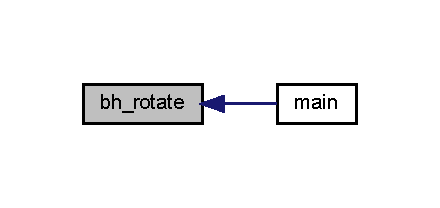
\includegraphics[width=211pt]{Marco_8f90_a6f9b11cb7ed99f525d6b03e1b3223dee_icgraph}
\end{center}
\end{figure}
\mbox{\Hypertarget{Marco_8f90_a88bc2c0947b2f1babf4dade8ee684423}\label{Marco_8f90_a88bc2c0947b2f1babf4dade8ee684423}} 
\index{Marco.\+f90@{Marco.\+f90}!bhc\+\_\+rotate@{bhc\+\_\+rotate}}
\index{bhc\+\_\+rotate@{bhc\+\_\+rotate}!Marco.\+f90@{Marco.\+f90}}
\subsubsection{\texorpdfstring{bhc\+\_\+rotate()}{bhc\_rotate()}}
{\footnotesize\ttfamily subroutine bhc\+\_\+rotate (\begin{DoxyParamCaption}\item[{integer}]{N\+F\+RQ,  }\item[{integer}]{L\+RX,  }\item[{integer}]{N\+T\+XE,  }\item[{integer, dimension(ntxe)}]{N\+R\+X\+TX,  }\item[{logical, dimension(lrx,ntxe)}]{B\+HR,  }\item[{real, dimension(lrx,ntxe)}]{D\+X\+AZ,  }\item[{real, dimension(lrx,ntxe)}]{D\+X\+D\+IP,  }\item[{complex, dimension(nfrq,lrx,ntxe,3)}]{B\+FD }\end{DoxyParamCaption})}

Here is the caller graph for this function\+:
\nopagebreak
\begin{figure}[H]
\begin{center}
\leavevmode
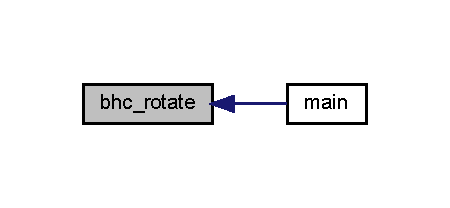
\includegraphics[width=216pt]{Marco_8f90_a88bc2c0947b2f1babf4dade8ee684423_icgraph}
\end{center}
\end{figure}
\mbox{\Hypertarget{Marco_8f90_a0df391e311aae0e0ab61a43fe99aa856}\label{Marco_8f90_a0df391e311aae0e0ab61a43fe99aa856}} 
\index{Marco.\+f90@{Marco.\+f90}!chk\+\_\+sym\+\_\+prop@{chk\+\_\+sym\+\_\+prop}}
\index{chk\+\_\+sym\+\_\+prop@{chk\+\_\+sym\+\_\+prop}!Marco.\+f90@{Marco.\+f90}}
\subsubsection{\texorpdfstring{chk\+\_\+sym\+\_\+prop()}{chk\_sym\_prop()}}
{\footnotesize\ttfamily subroutine chk\+\_\+symmetry\+::chk\+\_\+sym\+\_\+prop (\begin{DoxyParamCaption}\item[{integer}]{L1,  }\item[{integer}]{L2,  }\item[{real}]{N1,  }\item[{real}]{E1,  }\item[{integer}]{M\+A\+T\+CH }\end{DoxyParamCaption})}

Here is the caller graph for this function\+:
\nopagebreak
\begin{figure}[H]
\begin{center}
\leavevmode
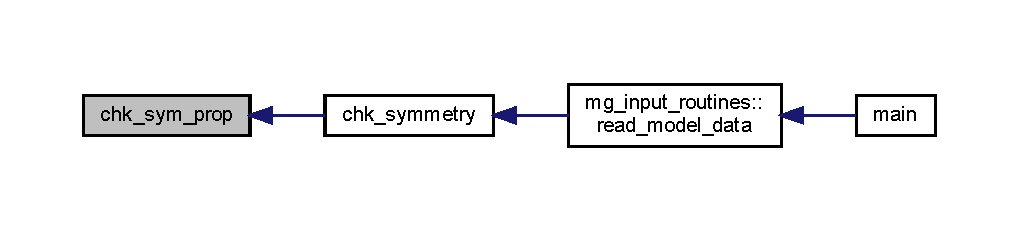
\includegraphics[width=350pt]{Marco_8f90_a0df391e311aae0e0ab61a43fe99aa856_icgraph}
\end{center}
\end{figure}
\mbox{\Hypertarget{Marco_8f90_a51e4a3fa9046596038f31e4e9a6ac7e5}\label{Marco_8f90_a51e4a3fa9046596038f31e4e9a6ac7e5}} 
\index{Marco.\+f90@{Marco.\+f90}!chk\+\_\+symmetry@{chk\+\_\+symmetry}}
\index{chk\+\_\+symmetry@{chk\+\_\+symmetry}!Marco.\+f90@{Marco.\+f90}}
\subsubsection{\texorpdfstring{chk\+\_\+symmetry()}{chk\_symmetry()}}
{\footnotesize\ttfamily subroutine chk\+\_\+symmetry (\begin{DoxyParamCaption}\item[{integer, intent(inout)}]{N\+P\+R\+I\+SM,  }\item[{integer, intent(in)}]{N\+P11,  }\item[{integer, dimension(np11,2), intent(inout)}]{L\+B\+LK,  }\item[{real, dimension(np11,9), intent(inout)}]{P\+B\+LK,  }\item[{real, intent(out)}]{TE,  }\item[{real, intent(out)}]{TN,  }\item[{integer, intent(out)}]{K\+S\+Y\+MM }\end{DoxyParamCaption})}

Here is the call graph for this function\+:
\nopagebreak
\begin{figure}[H]
\begin{center}
\leavevmode
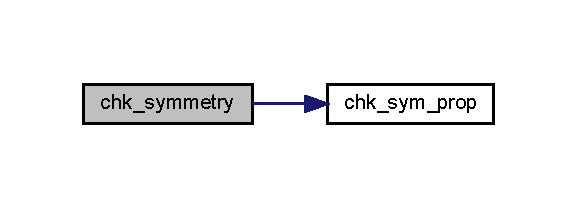
\includegraphics[width=277pt]{Marco_8f90_a51e4a3fa9046596038f31e4e9a6ac7e5_cgraph}
\end{center}
\end{figure}
Here is the caller graph for this function\+:
\nopagebreak
\begin{figure}[H]
\begin{center}
\leavevmode
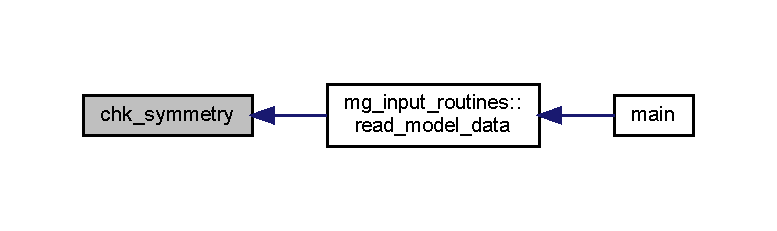
\includegraphics[width=350pt]{Marco_8f90_a51e4a3fa9046596038f31e4e9a6ac7e5_icgraph}
\end{center}
\end{figure}
\mbox{\Hypertarget{Marco_8f90_ad063b38dcbfa2382a1ed3380c8e53381}\label{Marco_8f90_ad063b38dcbfa2382a1ed3380c8e53381}} 
\index{Marco.\+f90@{Marco.\+f90}!compute\+\_\+3d@{compute\+\_\+3d}}
\index{compute\+\_\+3d@{compute\+\_\+3d}!Marco.\+f90@{Marco.\+f90}}
\subsubsection{\texorpdfstring{compute\+\_\+3d()}{compute\_3d()}}
{\footnotesize\ttfamily subroutine compute\+\_\+3d (\begin{DoxyParamCaption}\item[{integer, intent(in)}]{N\+F\+RQ,  }\item[{real, dimension(nfrq), intent(in)}]{F\+R\+EQ,  }\item[{integer, intent(in)}]{S\+O\+U\+R\+C\+E\+\_\+\+T\+Y\+PE,  }\item[{integer, intent(in)}]{NW,  }\item[{integer, intent(in)}]{N\+T\+XE,  }\item[{integer, intent(in)}]{N\+C\+RD,  }\item[{integer, dimension(ntxe), intent(in)}]{N\+\_\+\+V\+R\+TX,  }\item[{real, dimension(ncrd,ntxe), intent(in)}]{T\+X\+\_\+\+C\+R\+DX,  }\item[{real, dimension(ncrd,ntxe), intent(in)}]{T\+X\+\_\+\+C\+R\+DY,  }\item[{real, dimension(ncrd,ntxe), intent(in)}]{T\+X\+\_\+\+C\+R\+DZ,  }\item[{real, dimension(2,ntxe), intent(in)}]{M\+D\+\_\+\+A\+N\+G\+LE,  }\item[{integer, dimension(m\+\_\+rx,ntxe), intent(in)}]{R\+X\+\_\+\+T\+Y\+P\+E\+\_\+\+I\+N\+D\+EX,  }\item[{integer, dimension(m\+\_\+rx,ntxe), intent(in)}]{N\+\_\+\+S\+U\+B\+\_\+\+RX,  }\item[{real, dimension(3,sub\+\_\+rx\+\_\+max,m\+\_\+rx,ntxe), intent(in)}]{R\+X\+\_\+\+W\+E\+I\+G\+HT,  }\item[{integer, intent(in)}]{M\+\_\+\+RX,  }\item[{integer, dimension(ntxe), intent(in)}]{N\+\_\+\+RX,  }\item[{real, dimension(sub\+\_\+rx\+\_\+max,m\+\_\+rx,ntxe), intent(in)}]{R\+X\+\_\+X,  }\item[{real, dimension(sub\+\_\+rx\+\_\+max,m\+\_\+rx,ntxe), intent(in)}]{R\+X\+\_\+Y,  }\item[{real, dimension(sub\+\_\+rx\+\_\+max,m\+\_\+rx,ntxe), intent(in)}]{R\+X\+\_\+Z,  }\item[{integer, intent(in)}]{S\+U\+B\+\_\+\+R\+X\+\_\+\+M\+AX,  }\item[{integer, intent(in)}]{M\+L\+A\+Y\+ER,  }\item[{real, dimension(mlayer), intent(in)}]{L\+R\+Y\+TH,  }\item[{real, dimension(mlayer), intent(in)}]{R\+E\+S\+\_\+\+L\+YR,  }\item[{real, dimension(mlayer), intent(in)}]{R\+M\+U\+\_\+\+L\+YR,  }\item[{real, dimension(mlayer), intent(in)}]{R\+E\+S\+P\+\_\+\+L\+YR,  }\item[{real, dimension(mlayer), intent(in)}]{C\+H\+R\+G\+\_\+\+L\+YR,  }\item[{real, dimension(mlayer), intent(in)}]{T\+A\+U\+\_\+\+L\+YR,  }\item[{real, dimension(mlayer), intent(in)}]{F\+R\+Q\+C\+\_\+\+L\+YR,  }\item[{integer, intent(in)}]{D\+O3D,  }\item[{integer, intent(in)}]{S\+O\+L\+V\+ER,  }\item[{integer, intent(in)}]{K\+A\+CC,  }\item[{integer, intent(in)}]{K\+S\+Y\+MM,  }\item[{integer, intent(in)}]{T\+R\+G\+T\+\_\+\+B\+L\+CK,  }\item[{integer, dimension(trgt\+\_\+blck), intent(in)}]{B\+L\+C\+K\+\_\+\+NX,  }\item[{integer, dimension(trgt\+\_\+blck), intent(in)}]{B\+L\+C\+K\+\_\+\+NY,  }\item[{integer, dimension(trgt\+\_\+blck), intent(in)}]{B\+L\+C\+K\+\_\+\+NZ,  }\item[{real, dimension(trgt\+\_\+blck), intent(in)}]{B\+L\+C\+K\+\_\+\+LX,  }\item[{real, dimension(trgt\+\_\+blck), intent(in)}]{B\+L\+C\+K\+\_\+\+LY,  }\item[{real, dimension(trgt\+\_\+blck), intent(in)}]{B\+L\+C\+K\+\_\+\+LZ,  }\item[{real, dimension(trgt\+\_\+blck), intent(in)}]{B\+L\+C\+K\+\_\+\+CX,  }\item[{real, dimension(trgt\+\_\+blck), intent(in)}]{B\+L\+C\+K\+\_\+\+CY,  }\item[{real, dimension(trgt\+\_\+blck), intent(in)}]{B\+L\+C\+K\+\_\+\+CZ,  }\item[{real, dimension(trgt\+\_\+blck), intent(in)}]{R\+SB,  }\item[{real, dimension(trgt\+\_\+blck), intent(in)}]{C\+H\+R\+SB,  }\item[{real, dimension(trgt\+\_\+blck), intent(in)}]{T\+A\+U\+SB,  }\item[{real, dimension(trgt\+\_\+blck), intent(in)}]{C\+F\+R\+SB,  }\item[{real, dimension(trgt\+\_\+blck), intent(in)}]{R\+M\+UP,  }\item[{real, dimension(trgt\+\_\+blck), intent(in)}]{R\+E\+P\+SP,  }\item[{integer, intent(in)}]{E\+\_\+\+O\+N\+LY,  }\item[{complex, dimension(m\+\_\+rx,ntxe,nfrq), intent(out)}]{E\+PX,  }\item[{complex, dimension(m\+\_\+rx,ntxe,nfrq), intent(out)}]{E\+PY,  }\item[{complex, dimension(m\+\_\+rx,ntxe,nfrq), intent(out)}]{E\+PZ,  }\item[{complex, dimension(m\+\_\+rx,ntxe,nfrq), intent(out)}]{H\+PX,  }\item[{complex, dimension(m\+\_\+rx,ntxe,nfrq), intent(out)}]{H\+PY,  }\item[{complex, dimension(m\+\_\+rx,ntxe,nfrq), intent(out)}]{H\+PZ,  }\item[{complex, dimension(m\+\_\+rx,ntxe,nfrq), intent(out)}]{V\+O\+L\+TP,  }\item[{complex, dimension(m\+\_\+rx,ntxe,nfrq), intent(out)}]{E3X,  }\item[{complex, dimension(m\+\_\+rx,ntxe,nfrq), intent(out)}]{E3Y,  }\item[{complex, dimension(m\+\_\+rx,ntxe,nfrq), intent(out)}]{E3Z,  }\item[{complex, dimension(m\+\_\+rx,ntxe,nfrq), intent(out)}]{H3X,  }\item[{complex, dimension(m\+\_\+rx,ntxe,nfrq), intent(out)}]{H3Y,  }\item[{complex, dimension(m\+\_\+rx,ntxe,nfrq), intent(out)}]{H3Z,  }\item[{complex, dimension(m\+\_\+rx,ntxe,nfrq), intent(out)}]{V\+O\+L\+T3 }\end{DoxyParamCaption})}

Here is the call graph for this function\+:
\nopagebreak
\begin{figure}[H]
\begin{center}
\leavevmode
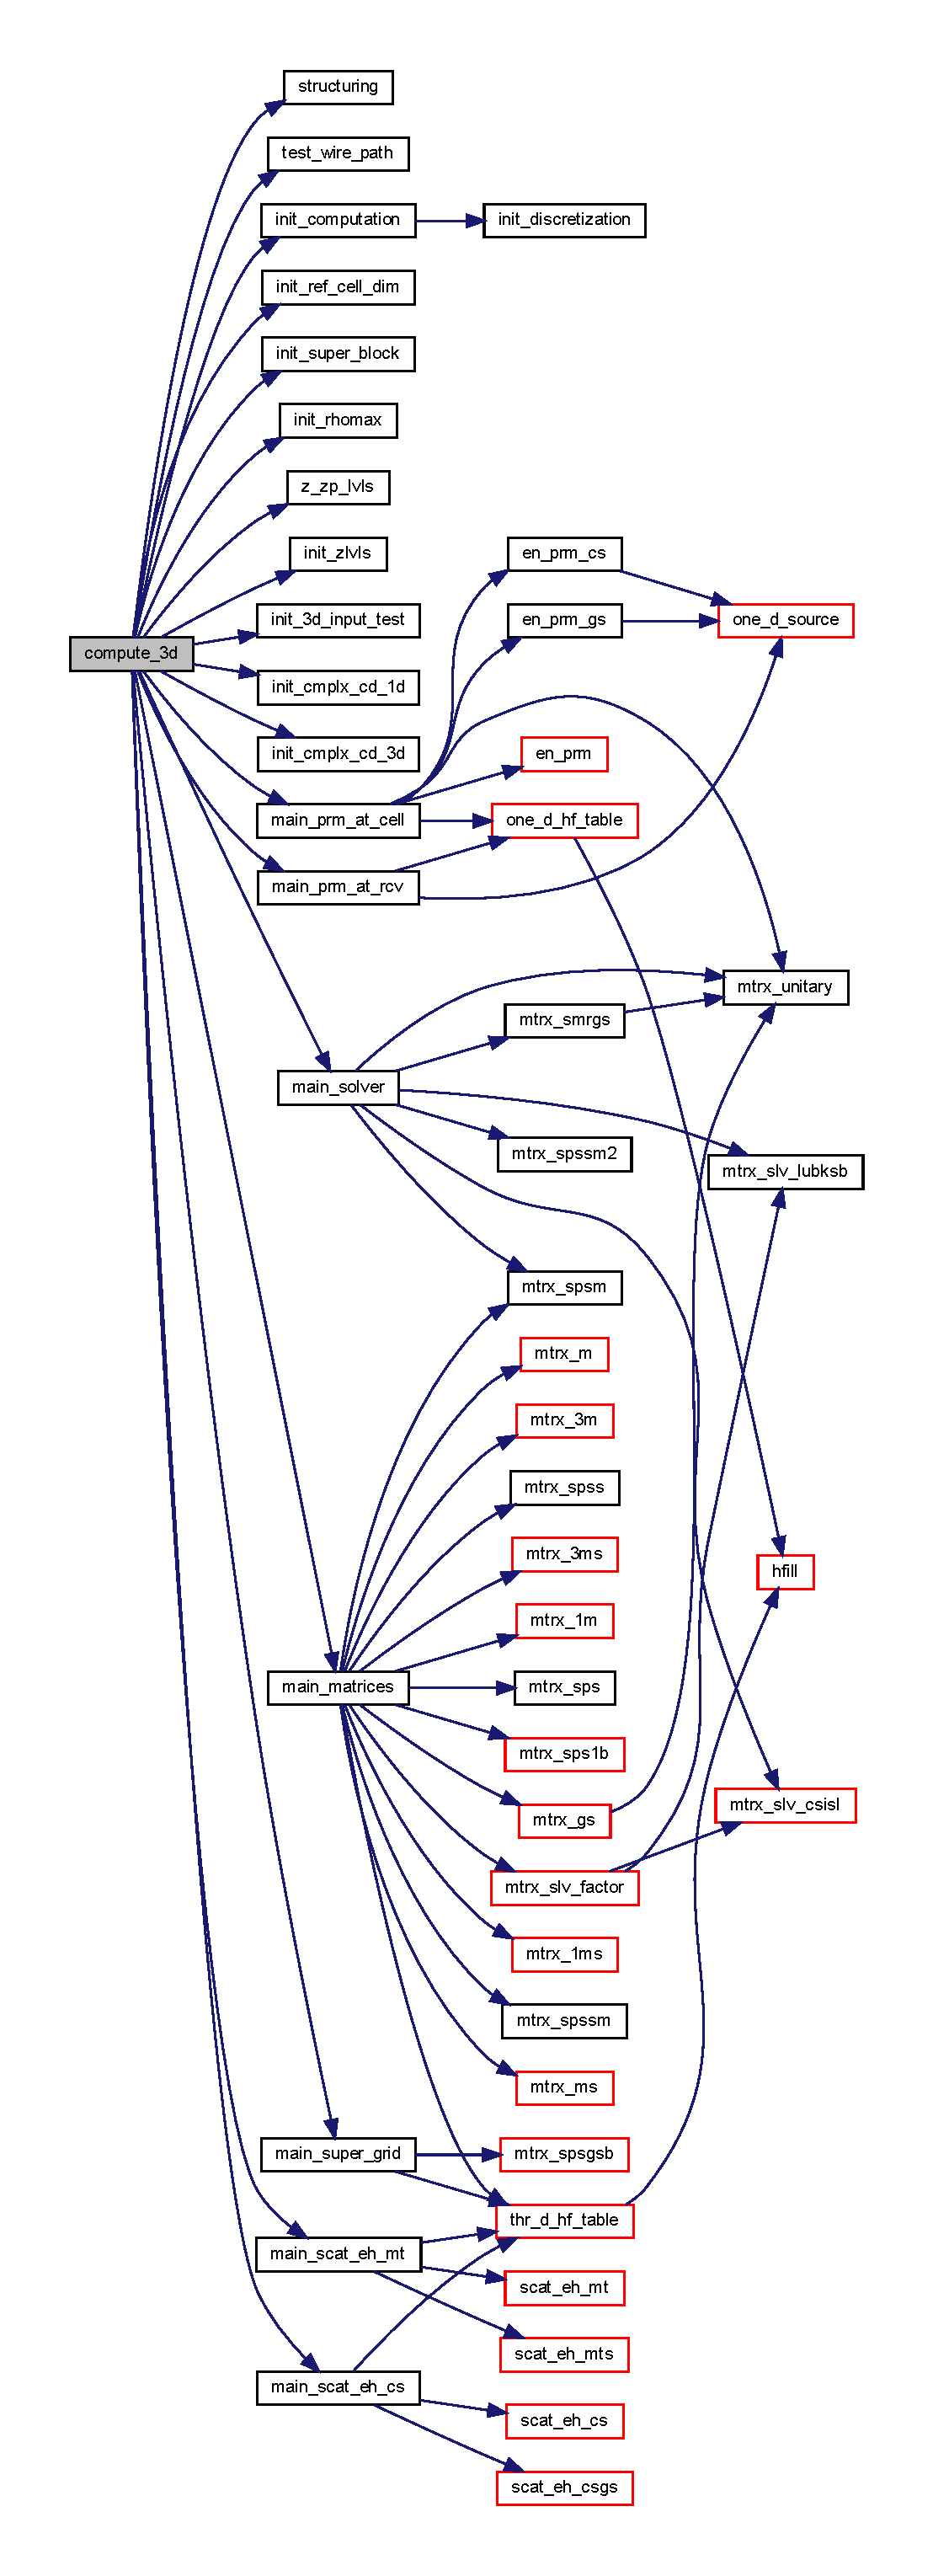
\includegraphics[height=550pt]{Marco_8f90_ad063b38dcbfa2382a1ed3380c8e53381_cgraph}
\end{center}
\end{figure}
Here is the caller graph for this function\+:
\nopagebreak
\begin{figure}[H]
\begin{center}
\leavevmode
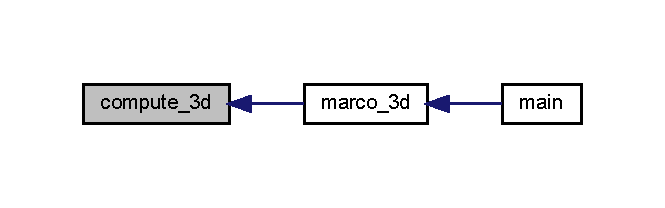
\includegraphics[width=319pt]{Marco_8f90_ad063b38dcbfa2382a1ed3380c8e53381_icgraph}
\end{center}
\end{figure}
\mbox{\Hypertarget{Marco_8f90_afc6a9dcc4e352b5f51fa8b7f42b6e1ad}\label{Marco_8f90_afc6a9dcc4e352b5f51fa8b7f42b6e1ad}} 
\index{Marco.\+f90@{Marco.\+f90}!costrn@{costrn}}
\index{costrn@{costrn}!Marco.\+f90@{Marco.\+f90}}
\subsubsection{\texorpdfstring{costrn()}{costrn()}}
{\footnotesize\ttfamily real function costrn (\begin{DoxyParamCaption}\item[{real, dimension(nfrq), intent(in)}]{WF,  }\item[{real, dimension(4,nfrq), intent(in)}]{Y\+F\+RQ,  }\item[{integer, intent(in)}]{N\+F\+RQ,  }\item[{integer}]{K\+F\+RQ,  }\item[{real, intent(in)}]{T }\end{DoxyParamCaption})}

\mbox{\Hypertarget{Marco_8f90_a0cebd439e7e54c21b37436ef4c5da9ca}\label{Marco_8f90_a0cebd439e7e54c21b37436ef4c5da9ca}} 
\index{Marco.\+f90@{Marco.\+f90}!cubint@{cubint}}
\index{cubint@{cubint}!Marco.\+f90@{Marco.\+f90}}
\subsubsection{\texorpdfstring{cubint()}{cubint()}}
{\footnotesize\ttfamily real function cubint (\begin{DoxyParamCaption}\item[{real, dimension(knot)}]{X\+K\+N\+OT,  }\item[{real, dimension(4,knot)}]{C\+O\+EF,  }\item[{integer}]{K\+N\+OT,  }\item[{real}]{X1,  }\item[{real}]{X2 }\end{DoxyParamCaption})}

Here is the call graph for this function\+:
\nopagebreak
\begin{figure}[H]
\begin{center}
\leavevmode
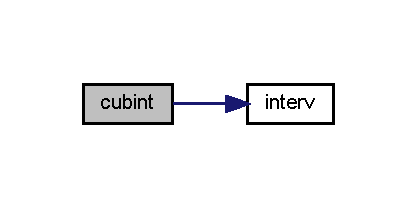
\includegraphics[width=200pt]{Marco_8f90_a0cebd439e7e54c21b37436ef4c5da9ca_cgraph}
\end{center}
\end{figure}
\mbox{\Hypertarget{Marco_8f90_a108ddb07c94297e8965b149f8e8b0b10}\label{Marco_8f90_a108ddb07c94297e8965b149f8e8b0b10}} 
\index{Marco.\+f90@{Marco.\+f90}!cubspl@{cubspl}}
\index{cubspl@{cubspl}!Marco.\+f90@{Marco.\+f90}}
\subsubsection{\texorpdfstring{cubspl()}{cubspl()}}
{\footnotesize\ttfamily subroutine cubspl (\begin{DoxyParamCaption}\item[{real, dimension(n), intent(in)}]{X\+N\+OT,  }\item[{real, dimension(4,n), intent(inout)}]{C,  }\item[{integer, intent(in)}]{N,  }\item[{integer, intent(in)}]{I\+B\+C\+B\+EG,  }\item[{integer, intent(in)}]{I\+B\+C\+E\+ND }\end{DoxyParamCaption})}

Here is the caller graph for this function\+:
\nopagebreak
\begin{figure}[H]
\begin{center}
\leavevmode
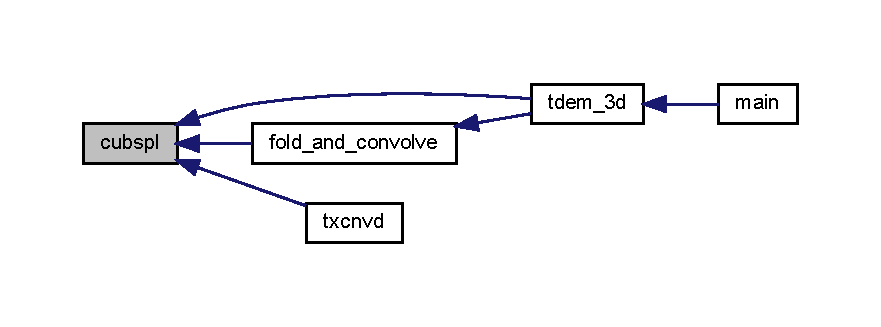
\includegraphics[width=350pt]{Marco_8f90_a108ddb07c94297e8965b149f8e8b0b10_icgraph}
\end{center}
\end{figure}
\mbox{\Hypertarget{Marco_8f90_ab1863f6d59c2ac8a89880c1b6cc8cbe9}\label{Marco_8f90_ab1863f6d59c2ac8a89880c1b6cc8cbe9}} 
\index{Marco.\+f90@{Marco.\+f90}!cubval@{cubval}}
\index{cubval@{cubval}!Marco.\+f90@{Marco.\+f90}}
\subsubsection{\texorpdfstring{cubval()}{cubval()}}
{\footnotesize\ttfamily real function cubval (\begin{DoxyParamCaption}\item[{real, dimension(knot), intent(in)}]{X\+K\+N\+OT,  }\item[{real, dimension(4,knot), intent(in)}]{C\+O\+EF,  }\item[{integer, intent(in)}]{K\+N\+OT,  }\item[{real, intent(in)}]{X1 }\end{DoxyParamCaption})}

Here is the call graph for this function\+:
\nopagebreak
\begin{figure}[H]
\begin{center}
\leavevmode
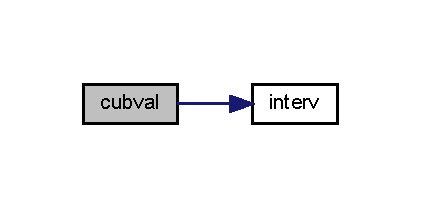
\includegraphics[width=202pt]{Marco_8f90_ab1863f6d59c2ac8a89880c1b6cc8cbe9_cgraph}
\end{center}
\end{figure}
\mbox{\Hypertarget{Marco_8f90_aa315629893313c49aa9f1836084f80b6}\label{Marco_8f90_aa315629893313c49aa9f1836084f80b6}} 
\index{Marco.\+f90@{Marco.\+f90}!en\+\_\+prm@{en\+\_\+prm}}
\index{en\+\_\+prm@{en\+\_\+prm}!Marco.\+f90@{Marco.\+f90}}
\subsubsection{\texorpdfstring{en\+\_\+prm()}{en\_prm()}}
{\footnotesize\ttfamily subroutine en\+\_\+prm (\begin{DoxyParamCaption}\item[{real}]{F\+RQ,  }\item[{integer}]{M\+L\+A\+Y\+ER,  }\item[{real, dimension(0\+:mlayer)}]{Z\+B\+ND,  }\item[{real, dimension(mlayer)}]{L\+R\+Y\+TH,  }\item[{complex, dimension(0\+:mlayer)}]{K\+KH,  }\item[{complex, dimension(0\+:mlayer)}]{C\+DH,  }\item[{integer}]{N\+ET,  }\item[{integer}]{S\+U\+B\+\_\+\+B\+L\+O\+CK,  }\item[{integer}]{N\+S\+U\+B\+CM,  }\item[{integer}]{N\+Z\+M\+AX,  }\item[{integer, dimension(sub\+\_\+block)}]{NX,  }\item[{integer, dimension(sub\+\_\+block)}]{NY,  }\item[{integer, dimension(sub\+\_\+block)}]{NZ,  }\item[{integer, dimension(sub\+\_\+block)}]{N\+C\+E\+LL,  }\item[{real, dimension(nzmax,sub\+\_\+block)}]{Z\+C\+E\+LL,  }\item[{complex, dimension(nsubcm,sub\+\_\+block)}]{C\+DB,  }\item[{integer}]{K\+P\+OL,  }\item[{complex, dimension(net)}]{EN,  }\item[{complex, dimension(net)}]{E\+CD }\end{DoxyParamCaption})}

Here is the call graph for this function\+:
\nopagebreak
\begin{figure}[H]
\begin{center}
\leavevmode
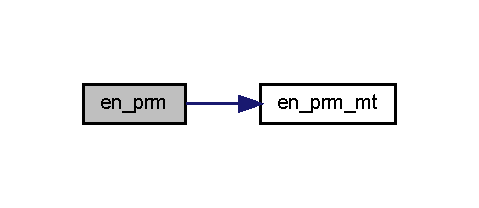
\includegraphics[width=230pt]{Marco_8f90_aa315629893313c49aa9f1836084f80b6_cgraph}
\end{center}
\end{figure}
Here is the caller graph for this function\+:
\nopagebreak
\begin{figure}[H]
\begin{center}
\leavevmode
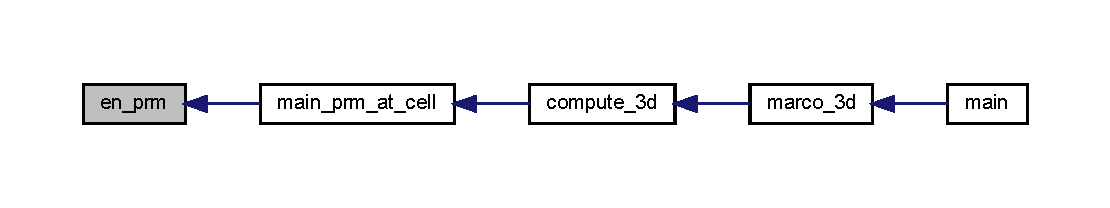
\includegraphics[width=350pt]{Marco_8f90_aa315629893313c49aa9f1836084f80b6_icgraph}
\end{center}
\end{figure}
\mbox{\Hypertarget{Marco_8f90_a18b8a51feece5566bf2eabdfec68c2b3}\label{Marco_8f90_a18b8a51feece5566bf2eabdfec68c2b3}} 
\index{Marco.\+f90@{Marco.\+f90}!en\+\_\+prm\+\_\+cs@{en\+\_\+prm\+\_\+cs}}
\index{en\+\_\+prm\+\_\+cs@{en\+\_\+prm\+\_\+cs}!Marco.\+f90@{Marco.\+f90}}
\subsubsection{\texorpdfstring{en\+\_\+prm\+\_\+cs()}{en\_prm\_cs()}}
{\footnotesize\ttfamily subroutine en\+\_\+prm\+\_\+cs (\begin{DoxyParamCaption}\item[{integer}]{N\+ET,  }\item[{integer}]{S\+U\+B\+\_\+\+B\+L\+O\+CK,  }\item[{integer}]{N\+S\+U\+B\+CM,  }\item[{integer}]{N\+X\+M\+AX,  }\item[{integer}]{N\+Y\+M\+AX,  }\item[{integer}]{N\+Z\+M\+AX,  }\item[{integer, dimension(sub\+\_\+block)}]{NX,  }\item[{integer, dimension(sub\+\_\+block)}]{NY,  }\item[{integer, dimension(sub\+\_\+block)}]{NZ,  }\item[{integer, dimension(sub\+\_\+block)}]{N\+C\+E\+LL,  }\item[{real, dimension(nxmax,sub\+\_\+block)}]{X\+C\+E\+LL,  }\item[{real, dimension(nymax,sub\+\_\+block)}]{Y\+C\+E\+LL,  }\item[{real, dimension(nzmax,sub\+\_\+block)}]{Z\+C\+E\+LL,  }\item[{complex, dimension(nsubcm,sub\+\_\+block)}]{C\+DB,  }\item[{integer}]{C\+S\+\_\+\+T\+Y\+PE,  }\item[{integer}]{N\+C\+RD,  }\item[{real, dimension(ncrd)}]{T\+X\+\_\+\+C\+R\+DX,  }\item[{real, dimension(ncrd)}]{T\+X\+\_\+\+C\+R\+DY,  }\item[{real, dimension(ncrd)}]{T\+X\+\_\+\+C\+R\+DZ,  }\item[{real}]{R\+AD,  }\item[{complex, dimension(net)}]{EN,  }\item[{complex, dimension(net)}]{E\+CD,  }\item[{real}]{F\+RQ,  }\item[{integer}]{M\+L\+A\+Y\+ER,  }\item[{real, dimension(0\+:mlayer)}]{Z\+B\+ND,  }\item[{complex, dimension(0\+:mlayer)}]{K\+KH,  }\item[{complex, dimension(0\+:mlayer)}]{C\+DH,  }\item[{real, dimension(2)}]{A\+N\+G\+L\+ES,  }\item[{integer}]{K\+E\+YG,  }\item[{integer}]{K\+A\+CC,  }\item[{real}]{AJ,  }\item[{integer}]{N\+Z\+OB,  }\item[{real, dimension(nzob)}]{Z\+O\+BG,  }\item[{integer}]{N\+Z\+SR,  }\item[{real, dimension(2,nzsr)}]{Z\+S\+RG,  }\item[{real}]{R\+H\+O\+M\+IN,  }\item[{integer}]{N\+H\+F\+I\+LM,  }\item[{real, dimension(nrg)}]{R\+RG,  }\item[{integer}]{N\+RG,  }\item[{complex, dimension(11,nhfilm,nzsr,nzob)}]{G\+R\+HF,  }\item[{complex, dimension(4,nzsr,nzob)}]{G\+R\+H\+O0 }\end{DoxyParamCaption})}

Here is the call graph for this function\+:
\nopagebreak
\begin{figure}[H]
\begin{center}
\leavevmode
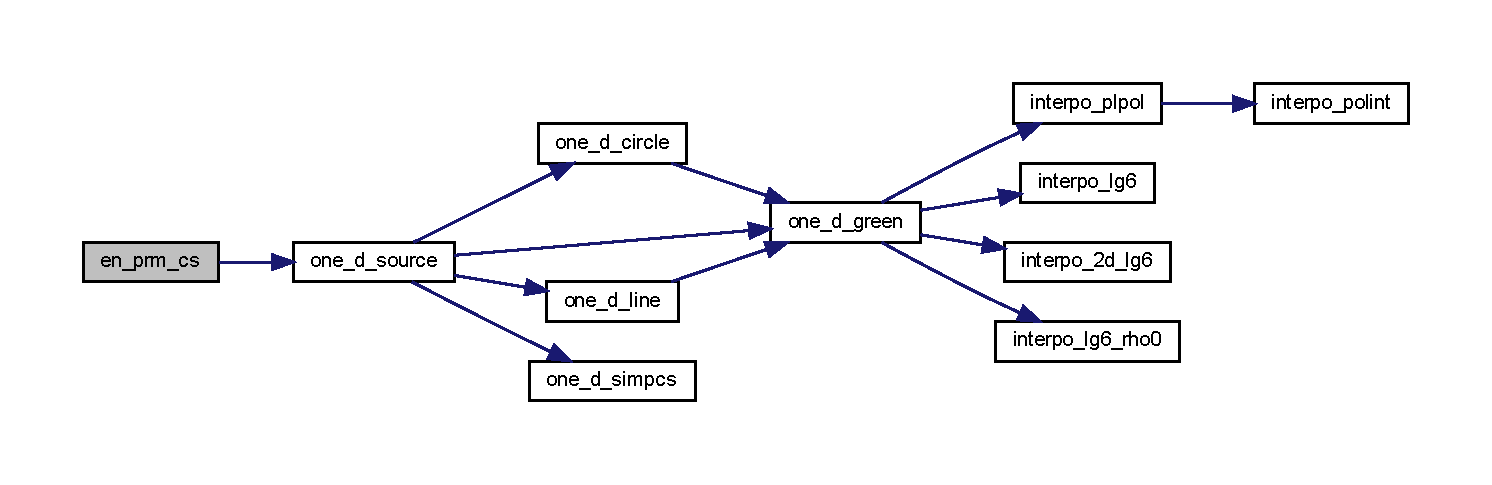
\includegraphics[width=350pt]{Marco_8f90_a18b8a51feece5566bf2eabdfec68c2b3_cgraph}
\end{center}
\end{figure}
Here is the caller graph for this function\+:
\nopagebreak
\begin{figure}[H]
\begin{center}
\leavevmode
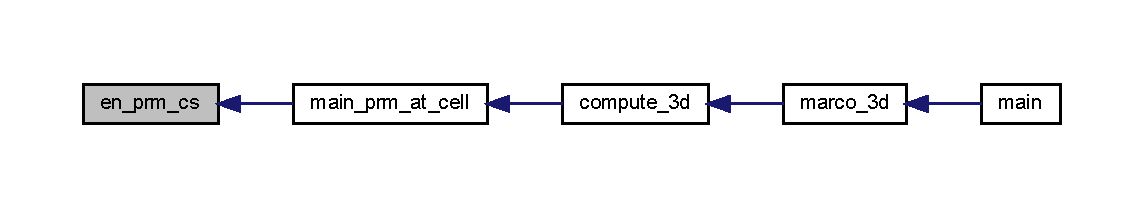
\includegraphics[width=350pt]{Marco_8f90_a18b8a51feece5566bf2eabdfec68c2b3_icgraph}
\end{center}
\end{figure}
\mbox{\Hypertarget{Marco_8f90_a6811caa6f5f24cf50a8f013171e9915c}\label{Marco_8f90_a6811caa6f5f24cf50a8f013171e9915c}} 
\index{Marco.\+f90@{Marco.\+f90}!en\+\_\+prm\+\_\+gs@{en\+\_\+prm\+\_\+gs}}
\index{en\+\_\+prm\+\_\+gs@{en\+\_\+prm\+\_\+gs}!Marco.\+f90@{Marco.\+f90}}
\subsubsection{\texorpdfstring{en\+\_\+prm\+\_\+gs()}{en\_prm\_gs()}}
{\footnotesize\ttfamily subroutine en\+\_\+prm\+\_\+gs (\begin{DoxyParamCaption}\item[{integer}]{N\+EQ,  }\item[{integer}]{N\+B\+O\+DY,  }\item[{integer, dimension(nbody)}]{S\+U\+B\+\_\+\+B\+L\+O\+CK,  }\item[{integer}]{N\+B\+M\+AX,  }\item[{integer}]{N\+X\+M\+AX,  }\item[{integer}]{N\+Y\+M\+AX,  }\item[{integer}]{N\+Z\+M\+AX,  }\item[{integer, dimension(nbody)}]{N\+ET,  }\item[{integer, dimension(nbmax,nbody)}]{NX,  }\item[{integer, dimension(nbmax,nbody)}]{NY,  }\item[{integer, dimension(nbmax,nbody)}]{NZ,  }\item[{integer, dimension(nbmax,nbody)}]{N\+C\+E\+LL,  }\item[{real, dimension(nxmax,nbmax,nbody)}]{X\+C\+E\+LL,  }\item[{real, dimension(nymax,nbmax,nbody)}]{Y\+C\+E\+LL,  }\item[{real, dimension(nzmax,nbmax,nbody)}]{Z\+C\+E\+LL,  }\item[{integer}]{C\+S\+\_\+\+T\+Y\+PE,  }\item[{integer}]{N\+C\+RD,  }\item[{real, dimension(ncrd)}]{T\+X\+\_\+\+C\+R\+DX,  }\item[{real, dimension(ncrd)}]{T\+X\+\_\+\+C\+R\+DY,  }\item[{real, dimension(ncrd)}]{T\+X\+\_\+\+C\+R\+DZ,  }\item[{real}]{R\+AD,  }\item[{complex, dimension(neq$\ast$4)}]{EN,  }\item[{real}]{F\+RQ,  }\item[{integer}]{M\+L\+A\+Y\+ER,  }\item[{real, dimension(0\+:mlayer)}]{Z\+B\+ND,  }\item[{complex, dimension(0\+:mlayer)}]{K\+KH,  }\item[{complex, dimension(0\+:mlayer)}]{C\+DH,  }\item[{real, dimension(2)}]{A\+N\+G\+L\+ES,  }\item[{integer}]{K\+E\+YG,  }\item[{integer}]{K\+A\+CC,  }\item[{real}]{AJ,  }\item[{integer}]{N\+Z\+OB,  }\item[{real, dimension(nzob)}]{Z\+O\+BG,  }\item[{integer}]{N\+Z\+SR,  }\item[{real, dimension(2,nzsr)}]{Z\+S\+RG,  }\item[{real}]{R\+H\+O\+M\+IN,  }\item[{integer}]{N\+H\+F\+I\+LM,  }\item[{real, dimension(nrg)}]{R\+RG,  }\item[{integer}]{N\+RG,  }\item[{complex, dimension(11,nhfilm,nzsr,nzob)}]{G\+R\+HF,  }\item[{complex, dimension(4,nzsr,nzob)}]{G\+R\+H\+O0 }\end{DoxyParamCaption})}

Here is the call graph for this function\+:
\nopagebreak
\begin{figure}[H]
\begin{center}
\leavevmode
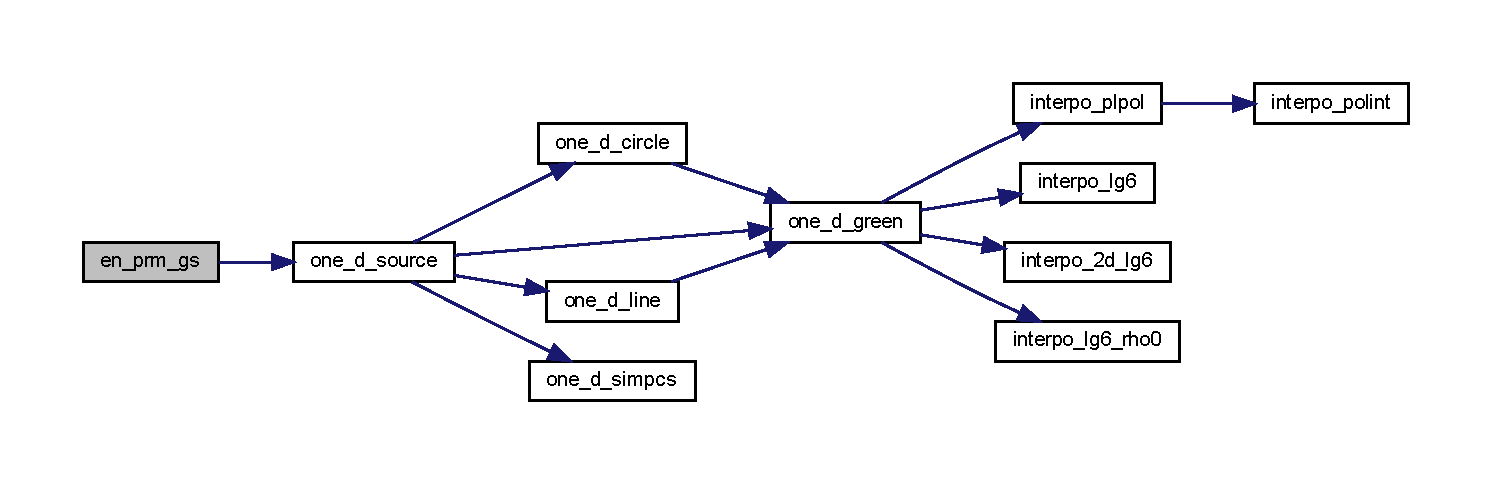
\includegraphics[width=350pt]{Marco_8f90_a6811caa6f5f24cf50a8f013171e9915c_cgraph}
\end{center}
\end{figure}
Here is the caller graph for this function\+:
\nopagebreak
\begin{figure}[H]
\begin{center}
\leavevmode
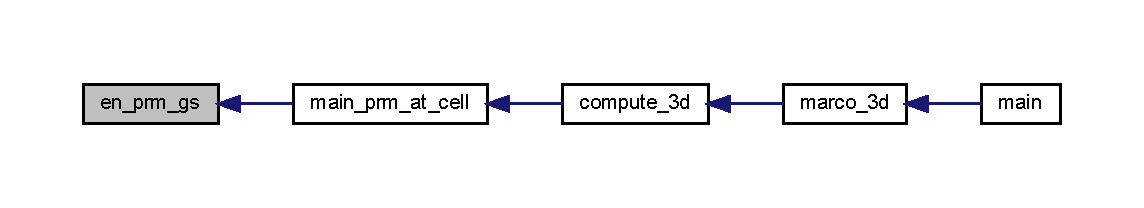
\includegraphics[width=350pt]{Marco_8f90_a6811caa6f5f24cf50a8f013171e9915c_icgraph}
\end{center}
\end{figure}
\mbox{\Hypertarget{Marco_8f90_a5cd1810beab2395c64ec9a3873337250}\label{Marco_8f90_a5cd1810beab2395c64ec9a3873337250}} 
\index{Marco.\+f90@{Marco.\+f90}!en\+\_\+prm\+\_\+mt@{en\+\_\+prm\+\_\+mt}}
\index{en\+\_\+prm\+\_\+mt@{en\+\_\+prm\+\_\+mt}!Marco.\+f90@{Marco.\+f90}}
\subsubsection{\texorpdfstring{en\+\_\+prm\+\_\+mt()}{en\_prm\_mt()}}
{\footnotesize\ttfamily subroutine en\+\_\+prm\+\_\+mt (\begin{DoxyParamCaption}\item[{real}]{F\+RQ,  }\item[{integer}]{M\+L\+A\+Y\+ER,  }\item[{real, dimension(0\+:mlayer)}]{Z\+B\+ND,  }\item[{real, dimension(mlayer)}]{L\+R\+Y\+TH,  }\item[{complex, dimension(0\+:mlayer)}]{K\+KH,  }\item[{integer}]{N\+O\+B\+SV,  }\item[{real}]{Z\+OB,  }\item[{complex}]{EX,  }\item[{complex}]{EY,  }\item[{complex}]{HX,  }\item[{complex}]{HY }\end{DoxyParamCaption})}

Here is the caller graph for this function\+:
\nopagebreak
\begin{figure}[H]
\begin{center}
\leavevmode
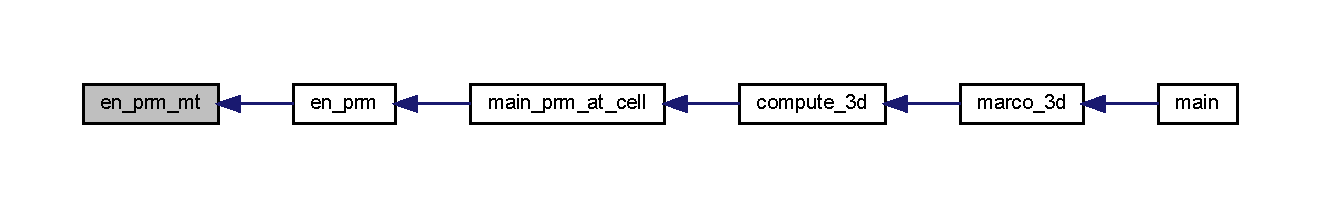
\includegraphics[width=350pt]{Marco_8f90_a5cd1810beab2395c64ec9a3873337250_icgraph}
\end{center}
\end{figure}
\mbox{\Hypertarget{Marco_8f90_a26a547e1b65b547041c0eac9e900a10d}\label{Marco_8f90_a26a547e1b65b547041c0eac9e900a10d}} 
\index{Marco.\+f90@{Marco.\+f90}!fd\+\_\+curnt@{fd\+\_\+curnt}}
\index{fd\+\_\+curnt@{fd\+\_\+curnt}!Marco.\+f90@{Marco.\+f90}}
\subsubsection{\texorpdfstring{fd\+\_\+curnt()}{fd\_curnt()}}
{\footnotesize\ttfamily subroutine fd\+\_\+curnt (\begin{DoxyParamCaption}\item[{integer}]{N\+F\+RQ,  }\item[{integer}]{L\+RX,  }\item[{integer}]{N\+T\+XE,  }\item[{real, dimension(nfrq)}]{C\+U\+R\+NT,  }\item[{complex, dimension(nfrq,lrx,ntxe,3)}]{R\+FD }\end{DoxyParamCaption})}

Here is the caller graph for this function\+:
\nopagebreak
\begin{figure}[H]
\begin{center}
\leavevmode
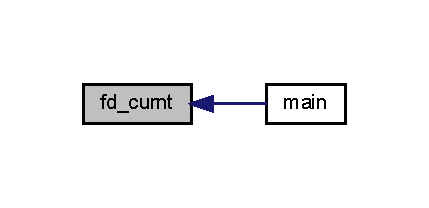
\includegraphics[width=206pt]{Marco_8f90_a26a547e1b65b547041c0eac9e900a10d_icgraph}
\end{center}
\end{figure}
\mbox{\Hypertarget{Marco_8f90_abbb41678ead372cf2ac619487c6fe732}\label{Marco_8f90_abbb41678ead372cf2ac619487c6fe732}} 
\index{Marco.\+f90@{Marco.\+f90}!fdread@{fdread}}
\index{fdread@{fdread}!Marco.\+f90@{Marco.\+f90}}
\subsubsection{\texorpdfstring{fdread()}{fdread()}}
{\footnotesize\ttfamily subroutine fdread (\begin{DoxyParamCaption}\item[{integer}]{ND,  }\item[{integer}]{N\+F\+RQ,  }\item[{integer}]{N\+T\+XE,  }\item[{integer}]{L\+RX,  }\item[{integer, dimension(ntxe)}]{N\+R\+X\+TX,  }\item[{integer, dimension(lrx,ntxe)}]{N\+C\+MP,  }\item[{complex, dimension(nfrq,lrx,ntxe,3)}]{B\+FD,  }\item[{complex, dimension(nfrq,lrx,ntxe,3)}]{B\+F\+D\+\_\+\+S\+C\+AT,  }\item[{integer}]{O\+U\+T\+P\+UT }\end{DoxyParamCaption})}

Here is the caller graph for this function\+:
\nopagebreak
\begin{figure}[H]
\begin{center}
\leavevmode
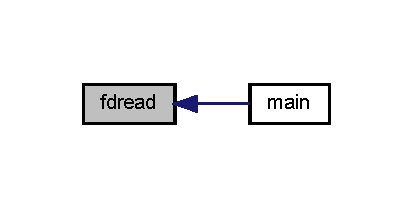
\includegraphics[width=198pt]{Marco_8f90_abbb41678ead372cf2ac619487c6fe732_icgraph}
\end{center}
\end{figure}
\mbox{\Hypertarget{Marco_8f90_afd1cc93ca825c04293fe19df43045f99}\label{Marco_8f90_afd1cc93ca825c04293fe19df43045f99}} 
\index{Marco.\+f90@{Marco.\+f90}!fem\+\_\+perc@{fem\+\_\+perc}}
\index{fem\+\_\+perc@{fem\+\_\+perc}!Marco.\+f90@{Marco.\+f90}}
\subsubsection{\texorpdfstring{fem\+\_\+perc()}{fem\_perc()}}
{\footnotesize\ttfamily subroutine fem\+\_\+perc (\begin{DoxyParamCaption}\item[{integer, intent(in)}]{N\+F\+RQ,  }\item[{integer, intent(in)}]{N\+S\+T\+NS,  }\item[{complex, dimension(nfrq, nstns), intent(in)}]{N\+UM,  }\item[{complex, dimension(nfrq, nstns), intent(in)}]{D\+EN,  }\item[{complex, dimension(nfrq, nstns), intent(out)}]{P\+RC }\end{DoxyParamCaption})}

Here is the caller graph for this function\+:
\nopagebreak
\begin{figure}[H]
\begin{center}
\leavevmode
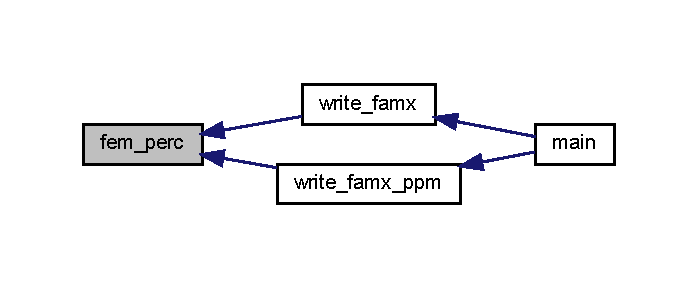
\includegraphics[width=335pt]{Marco_8f90_afd1cc93ca825c04293fe19df43045f99_icgraph}
\end{center}
\end{figure}
\mbox{\Hypertarget{Marco_8f90_adf5b72e5e0c8b51d6d076cc274531811}\label{Marco_8f90_adf5b72e5e0c8b51d6d076cc274531811}} 
\index{Marco.\+f90@{Marco.\+f90}!fold\+\_\+and\+\_\+convolve@{fold\+\_\+and\+\_\+convolve}}
\index{fold\+\_\+and\+\_\+convolve@{fold\+\_\+and\+\_\+convolve}!Marco.\+f90@{Marco.\+f90}}
\subsubsection{\texorpdfstring{fold\+\_\+and\+\_\+convolve()}{fold\_and\_convolve()}}
{\footnotesize\ttfamily subroutine fold\+\_\+and\+\_\+convolve (\begin{DoxyParamCaption}\item[{integer}]{S\+T\+E\+PC,  }\item[{integer}]{N\+SX,  }\item[{real, dimension(nsx)}]{S\+WX,  }\item[{real, dimension(nsx,3)}]{S\+WY,  }\item[{integer}]{N\+P\+U\+LS,  }\item[{real}]{P\+U\+L\+SE,  }\item[{real, dimension(ntyrp)}]{T\+RP,  }\item[{integer}]{N\+T\+Y\+RP,  }\item[{integer}]{N\+T\+Y\+P\+LS,  }\item[{integer}]{N\+C\+H\+NL,  }\item[{real, dimension(nchnl)}]{T\+O\+PN,  }\item[{real, dimension(nchnl)}]{T\+C\+LS,  }\item[{real, dimension(4,ntyrp)}]{Y\+P\+LS,  }\item[{real, dimension(nchnl)}]{Y\+C\+UM }\end{DoxyParamCaption})}

Here is the call graph for this function\+:
\nopagebreak
\begin{figure}[H]
\begin{center}
\leavevmode
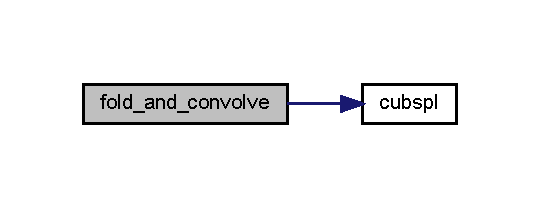
\includegraphics[width=259pt]{Marco_8f90_adf5b72e5e0c8b51d6d076cc274531811_cgraph}
\end{center}
\end{figure}
Here is the caller graph for this function\+:
\nopagebreak
\begin{figure}[H]
\begin{center}
\leavevmode
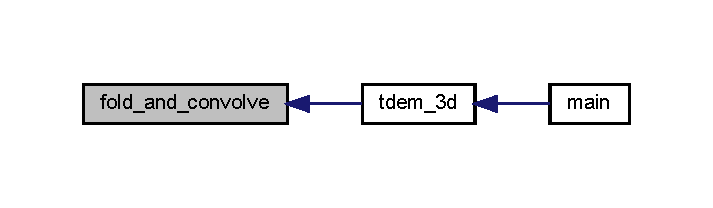
\includegraphics[width=342pt]{Marco_8f90_adf5b72e5e0c8b51d6d076cc274531811_icgraph}
\end{center}
\end{figure}
\mbox{\Hypertarget{Marco_8f90_a74a15aabfd889793f141e6d8ac9592c4}\label{Marco_8f90_a74a15aabfd889793f141e6d8ac9592c4}} 
\index{Marco.\+f90@{Marco.\+f90}!hfilh@{hfilh}}
\index{hfilh@{hfilh}!Marco.\+f90@{Marco.\+f90}}
\subsubsection{\texorpdfstring{hfilh()}{hfilh()}}
{\footnotesize\ttfamily subroutine hfilh (\begin{DoxyParamCaption}\item[{integer, intent(in)}]{K\+E\+YG,  }\item[{integer, intent(in)}]{K\+E\+MD,  }\item[{integer, intent(in)}]{M\+L\+A\+Y\+ER,  }\item[{real, dimension(0\+:mlayer), intent(in)}]{Z\+B\+ND,  }\item[{real, dimension(mlayer), intent(in)}]{L\+R\+Y\+TH,  }\item[{real, dimension(0\+:mlayer), intent(in)}]{H\+VK,  }\item[{complex, dimension(0\+:mlayer), intent(in)}]{K\+KH,  }\item[{integer, intent(in)}]{K\+A\+N\+IS,  }\item[{integer, intent(in)}]{K\+P\+RM,  }\item[{integer, intent(in)}]{K\+I\+TG,  }\item[{integer, intent(in)}]{K\+C\+H\+RG,  }\item[{integer, intent(in)}]{N\+OB,  }\item[{integer, intent(in)}]{N\+SR,  }\item[{real, intent(in)}]{R\+LO,  }\item[{real, intent(in)}]{R\+HI,  }\item[{real, intent(in)}]{Z\+OB,  }\item[{real, intent(in)}]{Z\+S\+RH,  }\item[{real, intent(in)}]{Z\+S\+RL,  }\item[{integer, intent(out)}]{N\+RG,  }\item[{real, dimension(nhfilm), intent(out)}]{R\+RG,  }\item[{complex, dimension(11,nhfilm), intent(out)}]{HF,  }\item[{integer, intent(in)}]{N\+H\+F\+I\+LM }\end{DoxyParamCaption})}

Here is the call graph for this function\+:
\nopagebreak
\begin{figure}[H]
\begin{center}
\leavevmode
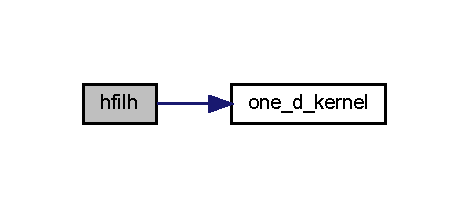
\includegraphics[width=225pt]{Marco_8f90_a74a15aabfd889793f141e6d8ac9592c4_cgraph}
\end{center}
\end{figure}
Here is the caller graph for this function\+:
\nopagebreak
\begin{figure}[H]
\begin{center}
\leavevmode
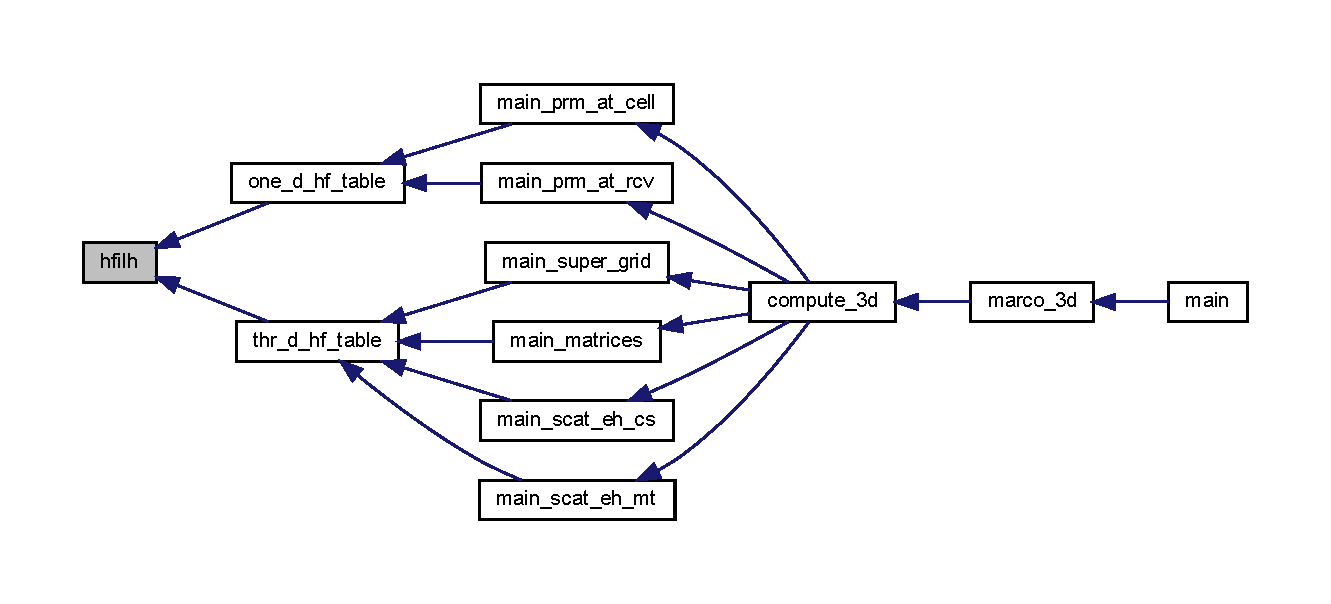
\includegraphics[width=350pt]{Marco_8f90_a74a15aabfd889793f141e6d8ac9592c4_icgraph}
\end{center}
\end{figure}
\mbox{\Hypertarget{Marco_8f90_a480d736c8998d27f049a30b17c5abb11}\label{Marco_8f90_a480d736c8998d27f049a30b17c5abb11}} 
\index{Marco.\+f90@{Marco.\+f90}!hfill@{hfill}}
\index{hfill@{hfill}!Marco.\+f90@{Marco.\+f90}}
\subsubsection{\texorpdfstring{hfill()}{hfill()}}
{\footnotesize\ttfamily subroutine hfill (\begin{DoxyParamCaption}\item[{integer, intent(in)}]{K\+E\+YG,  }\item[{integer, intent(in)}]{K\+E\+MD,  }\item[{integer, intent(in)}]{M\+L\+A\+Y\+ER,  }\item[{real, dimension(0\+:mlayer), intent(in)}]{Z\+B\+ND,  }\item[{real, dimension(mlayer), intent(in)}]{L\+R\+Y\+TH,  }\item[{real, dimension(0\+:mlayer), intent(in)}]{H\+VK,  }\item[{complex, dimension(0\+:mlayer), intent(in)}]{K\+KH,  }\item[{integer, intent(in)}]{K\+A\+N\+IS,  }\item[{integer, intent(in)}]{K\+P\+RM,  }\item[{integer, intent(in)}]{K\+I\+TG,  }\item[{integer, intent(in)}]{K\+C\+H\+RG,  }\item[{integer, intent(in)}]{N\+OB,  }\item[{integer, intent(in)}]{N\+SR,  }\item[{real, intent(in)}]{R\+LO,  }\item[{real, intent(in)}]{R\+HI,  }\item[{real, intent(in)}]{Z\+OB,  }\item[{real, intent(in)}]{Z\+S\+RH,  }\item[{real, intent(in)}]{Z\+S\+RL,  }\item[{integer, intent(out)}]{N\+RG,  }\item[{real, dimension(nhfilm), intent(out)}]{R\+RG,  }\item[{complex, dimension(11,nhfilm), intent(inout)}]{HF,  }\item[{integer, intent(in)}]{N\+H\+F\+I\+LM }\end{DoxyParamCaption})}

Here is the call graph for this function\+:
\nopagebreak
\begin{figure}[H]
\begin{center}
\leavevmode
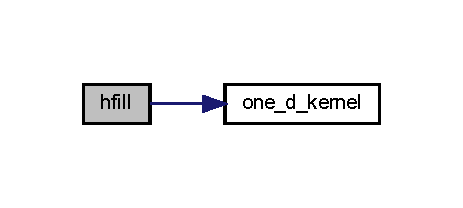
\includegraphics[width=222pt]{Marco_8f90_a480d736c8998d27f049a30b17c5abb11_cgraph}
\end{center}
\end{figure}
Here is the caller graph for this function\+:
\nopagebreak
\begin{figure}[H]
\begin{center}
\leavevmode
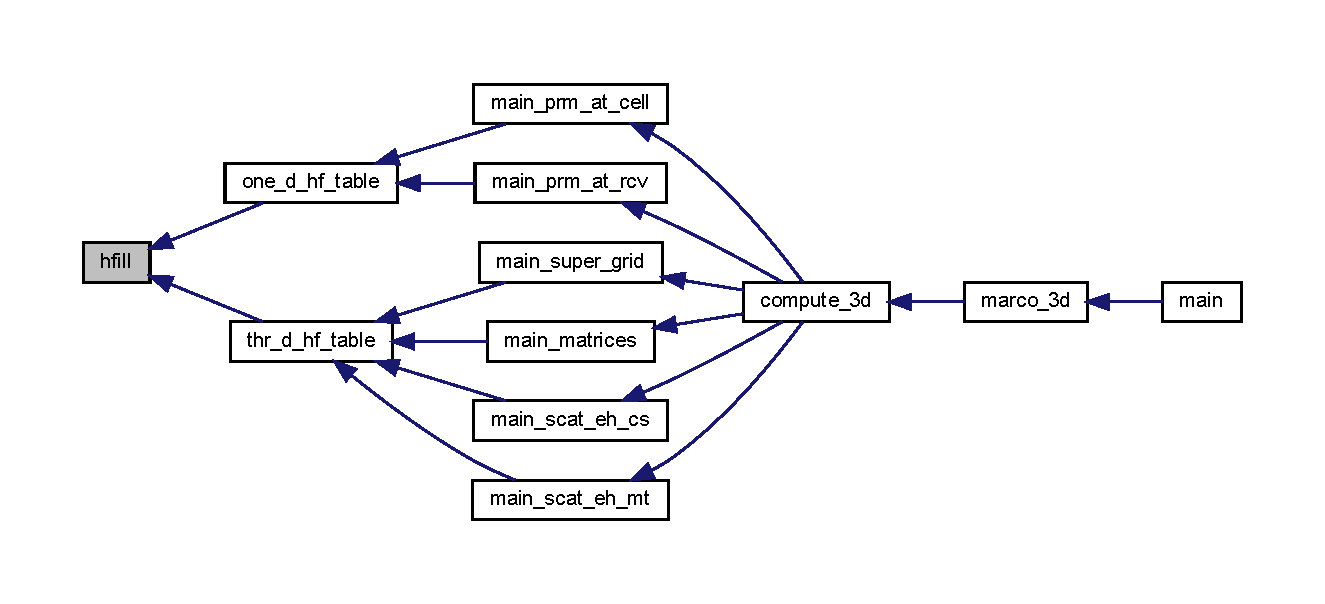
\includegraphics[width=350pt]{Marco_8f90_a480d736c8998d27f049a30b17c5abb11_icgraph}
\end{center}
\end{figure}
\mbox{\Hypertarget{Marco_8f90_afdb11dbe2b5041f4f314349b7334b974}\label{Marco_8f90_afdb11dbe2b5041f4f314349b7334b974}} 
\index{Marco.\+f90@{Marco.\+f90}!init\+\_\+3d\+\_\+input\+\_\+test@{init\+\_\+3d\+\_\+input\+\_\+test}}
\index{init\+\_\+3d\+\_\+input\+\_\+test@{init\+\_\+3d\+\_\+input\+\_\+test}!Marco.\+f90@{Marco.\+f90}}
\subsubsection{\texorpdfstring{init\+\_\+3d\+\_\+input\+\_\+test()}{init\_3d\_input\_test()}}
{\footnotesize\ttfamily subroutine init\+\_\+3d\+\_\+input\+\_\+test (\begin{DoxyParamCaption}\item[{integer}]{NW,  }\item[{integer}]{K\+A\+U\+TO,  }\item[{integer}]{K\+S\+Y\+MM,  }\item[{real}]{D\+M\+IN,  }\item[{integer}]{N\+S\+U\+B\+CM,  }\item[{integer}]{M\+B\+O\+DY,  }\item[{integer}]{N\+B\+M\+AX,  }\item[{integer}]{N\+X\+M\+AX,  }\item[{integer}]{N\+Y\+M\+AX,  }\item[{integer}]{N\+Z\+M\+AX,  }\item[{integer}]{N\+B\+O\+DY,  }\item[{integer}]{T\+R\+G\+T\+\_\+\+B\+L\+CK,  }\item[{real, dimension(trgt\+\_\+blck)}]{B\+L\+C\+K\+\_\+\+LX,  }\item[{real, dimension(trgt\+\_\+blck)}]{B\+L\+C\+K\+\_\+\+LY,  }\item[{real, dimension(trgt\+\_\+blck)}]{B\+L\+C\+K\+\_\+\+LZ,  }\item[{real, dimension(trgt\+\_\+blck)}]{B\+L\+C\+K\+\_\+\+CX,  }\item[{real, dimension(trgt\+\_\+blck)}]{B\+L\+C\+K\+\_\+\+CY,  }\item[{real, dimension(trgt\+\_\+blck)}]{B\+L\+C\+K\+\_\+\+CZ,  }\item[{integer, dimension(mbody)}]{N\+CT,  }\item[{integer, dimension(mbody)}]{S\+U\+B\+\_\+\+B\+L\+O\+CK,  }\item[{integer, dimension(nbmax,mbody)}]{NX,  }\item[{integer, dimension(nbmax,mbody)}]{NY,  }\item[{integer, dimension(nbmax,mbody)}]{NZ,  }\item[{real, dimension(nbmax,mbody)}]{B\+LX,  }\item[{real, dimension(nbmax,mbody)}]{B\+LY,  }\item[{real, dimension(nbmax,mbody)}]{B\+LZ,  }\item[{real, dimension(nbmax,mbody)}]{X\+BL,  }\item[{real, dimension(nbmax,mbody)}]{Y\+BL,  }\item[{real, dimension(nbmax,mbody)}]{Z\+BL,  }\item[{integer}]{M\+L\+A\+Y\+ER,  }\item[{real, dimension(0\+:mlayer)}]{Z\+B\+ND,  }\item[{real, dimension(nzmax,nbmax,mbody)}]{Z\+C\+E\+LL }\end{DoxyParamCaption})}

Here is the caller graph for this function\+:
\nopagebreak
\begin{figure}[H]
\begin{center}
\leavevmode
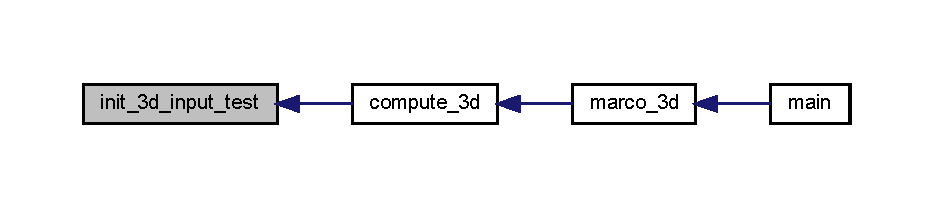
\includegraphics[width=350pt]{Marco_8f90_afdb11dbe2b5041f4f314349b7334b974_icgraph}
\end{center}
\end{figure}
\mbox{\Hypertarget{Marco_8f90_ab5e1d6b86ed64b774c25c5b69552f078}\label{Marco_8f90_ab5e1d6b86ed64b774c25c5b69552f078}} 
\index{Marco.\+f90@{Marco.\+f90}!init\+\_\+cmplx\+\_\+cd\+\_\+1d@{init\+\_\+cmplx\+\_\+cd\+\_\+1d}}
\index{init\+\_\+cmplx\+\_\+cd\+\_\+1d@{init\+\_\+cmplx\+\_\+cd\+\_\+1d}!Marco.\+f90@{Marco.\+f90}}
\subsubsection{\texorpdfstring{init\+\_\+cmplx\+\_\+cd\+\_\+1d()}{init\_cmplx\_cd\_1d()}}
{\footnotesize\ttfamily subroutine init\+\_\+cmplx\+\_\+cd\+\_\+1d (\begin{DoxyParamCaption}\item[{integer}]{NW,  }\item[{real}]{F\+RQ,  }\item[{integer}]{C\+O\+L\+E\+\_\+\+C\+O\+LE,  }\item[{integer}]{M\+L\+A\+Y\+ER,  }\item[{integer}]{K\+A\+N\+IS,  }\item[{real, dimension(0\+:mlayer)}]{H\+VK,  }\item[{real, dimension(mlayer)}]{R\+E\+S\+\_\+\+L\+YR,  }\item[{real, dimension(mlayer)}]{C\+H\+R\+G\+\_\+\+L\+YR,  }\item[{real, dimension(mlayer)}]{T\+A\+U\+\_\+\+L\+YR,  }\item[{real, dimension(mlayer)}]{F\+R\+Q\+C\+\_\+\+L\+YR,  }\item[{real, dimension(mlayer)}]{R\+M\+U\+\_\+\+L\+YR,  }\item[{real, dimension(mlayer)}]{R\+E\+S\+P\+\_\+\+L\+YR,  }\item[{real, dimension(mlayer)}]{D\+C\+H\+R\+G\+\_\+\+L\+YR,  }\item[{real, dimension(mlayer)}]{D\+T\+A\+U\+\_\+\+L\+YR,  }\item[{real, dimension(mlayer)}]{D\+F\+R\+Q\+C\+\_\+\+L\+YR,  }\item[{complex, dimension(0\+:mlayer)}]{C\+DH,  }\item[{complex, dimension(0\+:mlayer)}]{C\+DV,  }\item[{complex, dimension(0\+:mlayer)}]{K\+KH }\end{DoxyParamCaption})}

Here is the caller graph for this function\+:
\nopagebreak
\begin{figure}[H]
\begin{center}
\leavevmode
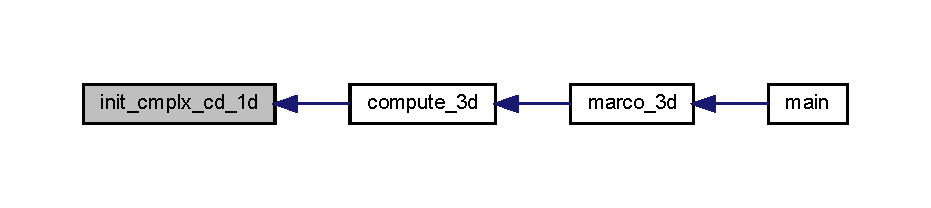
\includegraphics[width=350pt]{Marco_8f90_ab5e1d6b86ed64b774c25c5b69552f078_icgraph}
\end{center}
\end{figure}
\mbox{\Hypertarget{Marco_8f90_aaf5e8f1fe701ea6d58511ac2fabcd83c}\label{Marco_8f90_aaf5e8f1fe701ea6d58511ac2fabcd83c}} 
\index{Marco.\+f90@{Marco.\+f90}!init\+\_\+cmplx\+\_\+cd\+\_\+3d@{init\+\_\+cmplx\+\_\+cd\+\_\+3d}}
\index{init\+\_\+cmplx\+\_\+cd\+\_\+3d@{init\+\_\+cmplx\+\_\+cd\+\_\+3d}!Marco.\+f90@{Marco.\+f90}}
\subsubsection{\texorpdfstring{init\+\_\+cmplx\+\_\+cd\+\_\+3d()}{init\_cmplx\_cd\_3d()}}
{\footnotesize\ttfamily subroutine init\+\_\+cmplx\+\_\+cd\+\_\+3d (\begin{DoxyParamCaption}\item[{real}]{F\+RQ,  }\item[{integer}]{C\+O\+L\+E\+\_\+\+C\+O\+LE,  }\item[{integer}]{N\+B\+M\+AX,  }\item[{integer}]{N\+B\+O\+DY,  }\item[{integer, dimension(nbody)}]{S\+U\+B\+\_\+\+B\+L\+O\+CK,  }\item[{integer, dimension(nbmax,nbody)}]{N\+C\+E\+LL,  }\item[{real, dimension(nbmax,nbody)}]{B\+LZ,  }\item[{real, dimension(0\+:nlayer)}]{Z\+B\+ND,  }\item[{integer}]{N\+L\+A\+Y\+ER,  }\item[{real, dimension(nlayer)}]{R\+MU,  }\item[{integer}]{N\+S\+U\+B\+CM,  }\item[{complex, dimension(nsubcm,nbmax)}]{C\+DB,  }\item[{real, dimension(nbmax,nbody)}]{R\+BC,  }\item[{real, dimension(nbmax,nbody)}]{C\+H\+R\+BC,  }\item[{real, dimension(nbmax,nbody)}]{T\+A\+U\+BC,  }\item[{real, dimension(nbmax,nbody)}]{C\+F\+R\+BC,  }\item[{real, dimension(nbmax,nbody)}]{D\+E\+BC,  }\item[{real, dimension(nbmax,nbody)}]{R\+M\+UB }\end{DoxyParamCaption})}

Here is the caller graph for this function\+:
\nopagebreak
\begin{figure}[H]
\begin{center}
\leavevmode
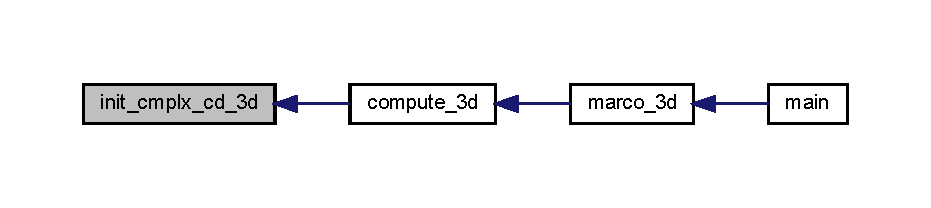
\includegraphics[width=350pt]{Marco_8f90_aaf5e8f1fe701ea6d58511ac2fabcd83c_icgraph}
\end{center}
\end{figure}
\mbox{\Hypertarget{Marco_8f90_a5f04384a88b1293a8d2dc26d86a77d08}\label{Marco_8f90_a5f04384a88b1293a8d2dc26d86a77d08}} 
\index{Marco.\+f90@{Marco.\+f90}!init\+\_\+computation@{init\+\_\+computation}}
\index{init\+\_\+computation@{init\+\_\+computation}!Marco.\+f90@{Marco.\+f90}}
\subsubsection{\texorpdfstring{init\+\_\+computation()}{init\_computation()}}
{\footnotesize\ttfamily subroutine init\+\_\+computation (\begin{DoxyParamCaption}\item[{real}]{D\+M\+IN,  }\item[{integer}]{M\+B\+O\+DY,  }\item[{integer}]{N\+B\+M\+AX,  }\item[{integer}]{N\+X\+M\+AX,  }\item[{integer}]{N\+Y\+M\+AX,  }\item[{integer}]{N\+Z\+M\+AX,  }\item[{integer}]{C\+S\+\_\+\+T\+Y\+PE,  }\item[{integer}]{K\+S\+Y\+MM,  }\item[{integer}]{N\+T\+XE,  }\item[{integer}]{S\+U\+B\+\_\+\+R\+X\+\_\+\+M\+AX,  }\item[{integer}]{M\+\_\+\+RX,  }\item[{integer, dimension(ntxe)}]{N\+\_\+\+RX,  }\item[{integer, dimension(m\+\_\+rx,ntxe)}]{N\+\_\+\+S\+U\+B\+\_\+\+RX,  }\item[{real, dimension(sub\+\_\+rx\+\_\+max,m\+\_\+rx,ntxe), intent(in)}]{R\+X\+\_\+X,  }\item[{real, dimension(sub\+\_\+rx\+\_\+max,m\+\_\+rx,ntxe), intent(in)}]{R\+X\+\_\+Y,  }\item[{real, dimension(sub\+\_\+rx\+\_\+max,m\+\_\+rx,ntxe), intent(in)}]{R\+X\+\_\+Z,  }\item[{real}]{Z\+MT,  }\item[{integer}]{M\+T\+\_\+\+P\+R\+O\+FL,  }\item[{integer}]{M\+T\+\_\+\+S\+T\+A\+TN,  }\item[{real, dimension(mt\+\_\+profl)}]{X\+R\+MT,  }\item[{real, dimension(mt\+\_\+statn)}]{Y\+R\+MT,  }\item[{integer}]{N\+B\+O\+DY,  }\item[{integer, dimension(mbody)}]{S\+U\+B\+\_\+\+B\+L\+O\+CK,  }\item[{integer, dimension(nbmax,mbody)}]{NX,  }\item[{integer, dimension(nbmax,mbody)}]{NY,  }\item[{integer, dimension(nbmax,mbody)}]{NZ,  }\item[{real, dimension(nbmax,mbody)}]{B\+LX,  }\item[{real, dimension(nbmax,mbody)}]{B\+LY,  }\item[{real, dimension(nbmax,mbody)}]{B\+LZ,  }\item[{real, dimension(nbmax,mbody)}]{X\+BL,  }\item[{real, dimension(nbmax,mbody)}]{Y\+BL,  }\item[{real, dimension(nbmax,mbody)}]{Z\+BL,  }\item[{real, dimension(nxmax)}]{X1,  }\item[{real, dimension(nymax)}]{Y1,  }\item[{real, dimension(nzmax)}]{Z1,  }\item[{integer, dimension(mbody)}]{N\+CT,  }\item[{integer, dimension(mbody)}]{N\+ET,  }\item[{integer, dimension(nbmax,mbody)}]{N\+C\+E\+LL,  }\item[{integer}]{N\+C\+TT,  }\item[{integer}]{N\+EQ,  }\item[{real, dimension(nxmax,nbmax,mbody)}]{X\+C\+E\+LL,  }\item[{real, dimension(nymax,nbmax,mbody)}]{Y\+C\+E\+LL,  }\item[{real, dimension(nzmax,nbmax,mbody)}]{Z\+C\+E\+LL,  }\item[{integer, dimension(mbody)}]{K\+C\+E\+LL,  }\item[{integer}]{K\+B\+O\+U\+ND,  }\item[{integer}]{M\+L\+A\+Y\+ER,  }\item[{real, dimension(0\+:mlayer)}]{Z\+B\+ND,  }\item[{integer}]{K\+S\+FT,  }\item[{integer, dimension(nbmax,mbody)}]{K\+E\+Y\+SF,  }\item[{integer}]{K\+G\+HP,  }\item[{real}]{B\+L\+M\+IN }\end{DoxyParamCaption})}

Here is the call graph for this function\+:
\nopagebreak
\begin{figure}[H]
\begin{center}
\leavevmode
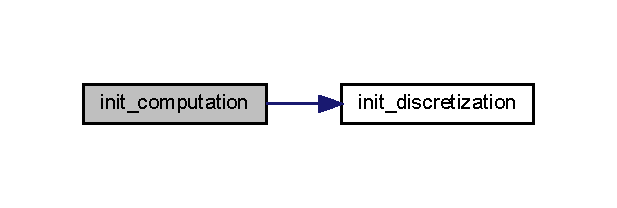
\includegraphics[width=296pt]{Marco_8f90_a5f04384a88b1293a8d2dc26d86a77d08_cgraph}
\end{center}
\end{figure}
Here is the caller graph for this function\+:
\nopagebreak
\begin{figure}[H]
\begin{center}
\leavevmode
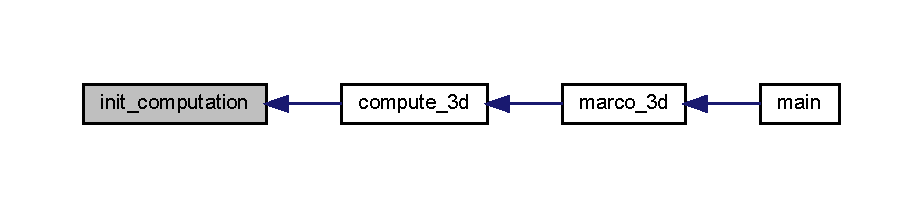
\includegraphics[width=350pt]{Marco_8f90_a5f04384a88b1293a8d2dc26d86a77d08_icgraph}
\end{center}
\end{figure}
\mbox{\Hypertarget{Marco_8f90_aca2a0c5479ec07e65782fa62da433365}\label{Marco_8f90_aca2a0c5479ec07e65782fa62da433365}} 
\index{Marco.\+f90@{Marco.\+f90}!init\+\_\+discretization@{init\+\_\+discretization}}
\index{init\+\_\+discretization@{init\+\_\+discretization}!Marco.\+f90@{Marco.\+f90}}
\subsubsection{\texorpdfstring{init\+\_\+discretization()}{init\_discretization()}}
{\footnotesize\ttfamily subroutine init\+\_\+discretization (\begin{DoxyParamCaption}\item[{real}]{B\+LX,  }\item[{real}]{B\+LY,  }\item[{real}]{B\+LZ,  }\item[{integer}]{NX,  }\item[{integer}]{NY,  }\item[{integer}]{NZ,  }\item[{real}]{X\+CD,  }\item[{real}]{Y\+CD,  }\item[{real}]{Z\+CD,  }\item[{real, dimension(nx)}]{X,  }\item[{real, dimension(ny)}]{Y,  }\item[{real, dimension(nz)}]{Z }\end{DoxyParamCaption})}

Here is the caller graph for this function\+:
\nopagebreak
\begin{figure}[H]
\begin{center}
\leavevmode
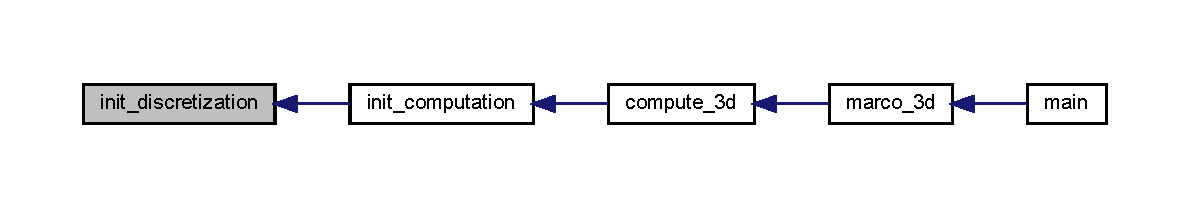
\includegraphics[width=350pt]{Marco_8f90_aca2a0c5479ec07e65782fa62da433365_icgraph}
\end{center}
\end{figure}
\mbox{\Hypertarget{Marco_8f90_abe7f527d74ea96643956d52265c43729}\label{Marco_8f90_abe7f527d74ea96643956d52265c43729}} 
\index{Marco.\+f90@{Marco.\+f90}!init\+\_\+ref\+\_\+cell\+\_\+dim@{init\+\_\+ref\+\_\+cell\+\_\+dim}}
\index{init\+\_\+ref\+\_\+cell\+\_\+dim@{init\+\_\+ref\+\_\+cell\+\_\+dim}!Marco.\+f90@{Marco.\+f90}}
\subsubsection{\texorpdfstring{init\+\_\+ref\+\_\+cell\+\_\+dim()}{init\_ref\_cell\_dim()}}
{\footnotesize\ttfamily subroutine init\+\_\+ref\+\_\+cell\+\_\+dim (\begin{DoxyParamCaption}\item[{integer}]{NW,  }\item[{integer}]{M\+B\+O\+DY,  }\item[{integer}]{N\+B\+M\+AX,  }\item[{integer}]{N\+B\+O\+DY,  }\item[{integer, dimension(mbody)}]{S\+U\+B\+\_\+\+B\+L\+O\+CK,  }\item[{real, dimension(nbmax,mbody)}]{B\+LX,  }\item[{real, dimension(nbmax,mbody)}]{B\+LY,  }\item[{real, dimension(nbmax,mbody)}]{B\+LZ,  }\item[{real}]{D\+M\+IN,  }\item[{integer}]{K\+C\+L\+MN,  }\item[{real, dimension(mbody)}]{C\+L\+MN }\end{DoxyParamCaption})}

Here is the caller graph for this function\+:
\nopagebreak
\begin{figure}[H]
\begin{center}
\leavevmode
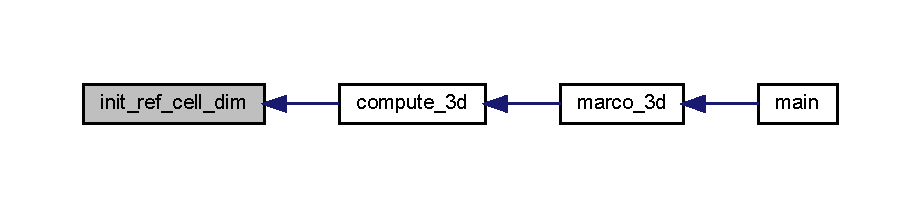
\includegraphics[width=350pt]{Marco_8f90_abe7f527d74ea96643956d52265c43729_icgraph}
\end{center}
\end{figure}
\mbox{\Hypertarget{Marco_8f90_a0ba9e9f35837a34d8df25a815723376a}\label{Marco_8f90_a0ba9e9f35837a34d8df25a815723376a}} 
\index{Marco.\+f90@{Marco.\+f90}!init\+\_\+rhomax@{init\+\_\+rhomax}}
\index{init\+\_\+rhomax@{init\+\_\+rhomax}!Marco.\+f90@{Marco.\+f90}}
\subsubsection{\texorpdfstring{init\+\_\+rhomax()}{init\_rhomax()}}
{\footnotesize\ttfamily subroutine init\+\_\+rhomax (\begin{DoxyParamCaption}\item[{integer}]{D\+O3D,  }\item[{integer}]{M\+B\+O\+DY,  }\item[{integer}]{N\+B\+M\+AX,  }\item[{integer}]{N\+X\+M\+AX,  }\item[{integer}]{N\+Y\+M\+AX,  }\item[{integer}]{K\+S\+Y\+MM,  }\item[{integer}]{N\+B\+O\+DY,  }\item[{integer, dimension(mbody)}]{S\+U\+B\+\_\+\+B\+L\+O\+CK,  }\item[{integer, dimension(nbmax,mbody)}]{NX,  }\item[{integer, dimension(nbmax,mbody)}]{NY,  }\item[{real, dimension(nxmax,nbmax,mbody)}]{X\+C\+E\+LL,  }\item[{real, dimension(nymax,nbmax,mbody)}]{Y\+C\+E\+LL,  }\item[{real, dimension(nbmax,mbody)}]{B\+LX,  }\item[{real, dimension(nbmax,mbody)}]{B\+LY,  }\item[{integer}]{N\+T\+XE,  }\item[{integer}]{N\+C\+RD,  }\item[{real, dimension(ncrd,ntxe)}]{T\+X\+\_\+\+C\+R\+DX,  }\item[{real, dimension(ncrd,ntxe)}]{T\+X\+\_\+\+C\+R\+DY,  }\item[{integer, dimension(ntxe)}]{N\+\_\+\+RX,  }\item[{real, dimension(sub\+\_\+rx\+\_\+max,m\+\_\+rx,ntxe)}]{R\+X\+\_\+X,  }\item[{real, dimension(sub\+\_\+rx\+\_\+max,m\+\_\+rx,ntxe)}]{R\+X\+\_\+Y,  }\item[{integer}]{S\+U\+B\+\_\+\+R\+X\+\_\+\+M\+AX,  }\item[{integer, dimension(m\+\_\+rx,ntxe)}]{N\+\_\+\+S\+U\+B\+\_\+\+RX,  }\item[{integer}]{M\+\_\+\+RX,  }\item[{real}]{R\+H\+O\+M\+IN,  }\item[{real}]{R\+M\+A\+X1,  }\item[{real}]{R\+M\+I\+N1,  }\item[{real}]{R\+M\+A\+X2,  }\item[{real}]{R\+M\+I\+N2 }\end{DoxyParamCaption})}

Here is the caller graph for this function\+:
\nopagebreak
\begin{figure}[H]
\begin{center}
\leavevmode
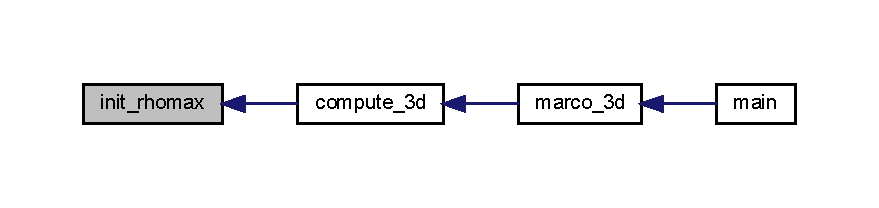
\includegraphics[width=350pt]{Marco_8f90_a0ba9e9f35837a34d8df25a815723376a_icgraph}
\end{center}
\end{figure}
\mbox{\Hypertarget{Marco_8f90_ac268fba86b567389312bb1f5945bec19}\label{Marco_8f90_ac268fba86b567389312bb1f5945bec19}} 
\index{Marco.\+f90@{Marco.\+f90}!init\+\_\+super\+\_\+block@{init\+\_\+super\+\_\+block}}
\index{init\+\_\+super\+\_\+block@{init\+\_\+super\+\_\+block}!Marco.\+f90@{Marco.\+f90}}
\subsubsection{\texorpdfstring{init\+\_\+super\+\_\+block()}{init\_super\_block()}}
{\footnotesize\ttfamily subroutine init\+\_\+super\+\_\+block (\begin{DoxyParamCaption}\item[{integer}]{NW,  }\item[{integer}]{M\+B\+O\+DY,  }\item[{integer}]{N\+B\+M\+AX,  }\item[{integer}]{N\+S\+MR,  }\item[{integer}]{K\+S\+Y\+MM,  }\item[{real}]{D\+M\+IN,  }\item[{integer}]{N\+X\+M\+AX,  }\item[{integer}]{N\+Y\+M\+AX,  }\item[{integer}]{N\+Z\+M\+AX,  }\item[{integer}]{N\+B\+O\+DY,  }\item[{integer, dimension(mbody)}]{S\+U\+B\+\_\+\+B\+L\+O\+CK,  }\item[{real, dimension(nbmax,mbody)}]{B\+LX,  }\item[{real, dimension(nbmax,mbody)}]{B\+LY,  }\item[{real, dimension(nbmax,mbody)}]{B\+LZ,  }\item[{integer, dimension(nbmax,mbody)}]{NX,  }\item[{integer, dimension(nbmax,mbody)}]{NY,  }\item[{integer, dimension(nbmax,mbody)}]{NZ,  }\item[{real, dimension(nbmax,mbody)}]{X\+BL,  }\item[{real, dimension(nbmax,mbody)}]{Y\+BL,  }\item[{real, dimension(nbmax,mbody)}]{Z\+BL,  }\item[{real, dimension(nxmax,nbmax,mbody)}]{X\+C\+E\+LL,  }\item[{real, dimension(nymax,nbmax,mbody)}]{Y\+C\+E\+LL,  }\item[{real, dimension(nzmax,nbmax,mbody)}]{Z\+C\+E\+LL,  }\item[{real}]{S\+BX,  }\item[{real}]{S\+BY,  }\item[{real}]{S\+BZ,  }\item[{real}]{X\+SB,  }\item[{real}]{Y\+SB,  }\item[{real}]{Z\+SB,  }\item[{real}]{S\+CX,  }\item[{real}]{S\+CY,  }\item[{real}]{S\+CZ,  }\item[{integer}]{N\+XS,  }\item[{integer}]{N\+YS,  }\item[{integer}]{N\+ZS,  }\item[{integer}]{K\+S\+MR }\end{DoxyParamCaption})}

Here is the caller graph for this function\+:
\nopagebreak
\begin{figure}[H]
\begin{center}
\leavevmode
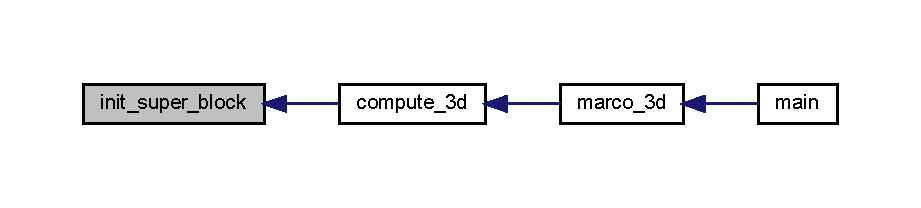
\includegraphics[width=350pt]{Marco_8f90_ac268fba86b567389312bb1f5945bec19_icgraph}
\end{center}
\end{figure}
\mbox{\Hypertarget{Marco_8f90_a4052ce4c8e8ce6ad657a5430196fb520}\label{Marco_8f90_a4052ce4c8e8ce6ad657a5430196fb520}} 
\index{Marco.\+f90@{Marco.\+f90}!init\+\_\+zlvls@{init\+\_\+zlvls}}
\index{init\+\_\+zlvls@{init\+\_\+zlvls}!Marco.\+f90@{Marco.\+f90}}
\subsubsection{\texorpdfstring{init\+\_\+zlvls()}{init\_zlvls()}}
{\footnotesize\ttfamily subroutine init\+\_\+zlvls (\begin{DoxyParamCaption}\item[{integer, intent(in)}]{NW,  }\item[{integer, intent(in)}]{M\+B\+O\+DY,  }\item[{integer, intent(in)}]{N\+B\+M\+AX,  }\item[{integer, intent(in)}]{N\+Z\+M\+AX,  }\item[{integer, intent(in)}]{K\+S\+MR,  }\item[{integer, intent(in)}]{N\+B\+O\+DY,  }\item[{integer, dimension(mbody), intent(in)}]{S\+U\+B\+\_\+\+B\+L\+O\+CK,  }\item[{integer, intent(in)}]{N\+ZS,  }\item[{integer, dimension(nbmax,mbody), intent(in)}]{NZ,  }\item[{real, intent(in)}]{S\+BZ,  }\item[{real, intent(in)}]{S\+CZ,  }\item[{real, intent(in)}]{Z\+SB,  }\item[{real, dimension(nzmax,nbmax,mbody), intent(in)}]{Z\+C\+E\+LL,  }\item[{real, dimension(nbmax,mbody), intent(in)}]{B\+LZ,  }\item[{integer, intent(in)}]{M\+Z\+G\+R\+ID,  }\item[{real, intent(in)}]{D\+M\+IN,  }\item[{integer, intent(out)}]{N\+Z\+SR,  }\item[{real, dimension(2,mzgrid), intent(out)}]{Z\+S\+RG,  }\item[{integer, intent(out)}]{N\+Z\+OB,  }\item[{real, dimension(mzgrid), intent(out)}]{Z\+O\+BG }\end{DoxyParamCaption})}

Here is the caller graph for this function\+:
\nopagebreak
\begin{figure}[H]
\begin{center}
\leavevmode
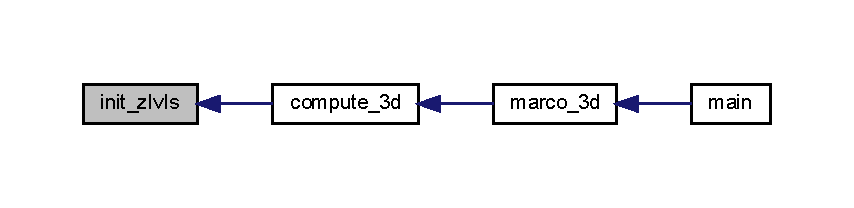
\includegraphics[width=350pt]{Marco_8f90_a4052ce4c8e8ce6ad657a5430196fb520_icgraph}
\end{center}
\end{figure}
\mbox{\Hypertarget{Marco_8f90_a170a0edeb8c14a416b4ec927bd0b5761}\label{Marco_8f90_a170a0edeb8c14a416b4ec927bd0b5761}} 
\index{Marco.\+f90@{Marco.\+f90}!interpo\+\_\+2d\+\_\+lg6@{interpo\+\_\+2d\+\_\+lg6}}
\index{interpo\+\_\+2d\+\_\+lg6@{interpo\+\_\+2d\+\_\+lg6}!Marco.\+f90@{Marco.\+f90}}
\subsubsection{\texorpdfstring{interpo\+\_\+2d\+\_\+lg6()}{interpo\_2d\_lg6()}}
{\footnotesize\ttfamily subroutine interpo\+\_\+2d\+\_\+lg6 (\begin{DoxyParamCaption}\item[{complex, dimension(11,nhfilm,nzsr,nzob)}]{G\+R\+HF,  }\item[{real, dimension(l)}]{A,  }\item[{integer}]{L,  }\item[{integer}]{N\+H\+F\+I\+LM,  }\item[{integer}]{N\+Z\+SR,  }\item[{integer}]{N\+Z\+OB,  }\item[{real}]{X,  }\item[{integer}]{I\+OB,  }\item[{real}]{Z\+SR,  }\item[{real, dimension(2,nzsr)}]{Z\+S\+RG,  }\item[{complex, dimension(nf)}]{F,  }\item[{integer}]{NF }\end{DoxyParamCaption})}

Here is the caller graph for this function\+:
\nopagebreak
\begin{figure}[H]
\begin{center}
\leavevmode
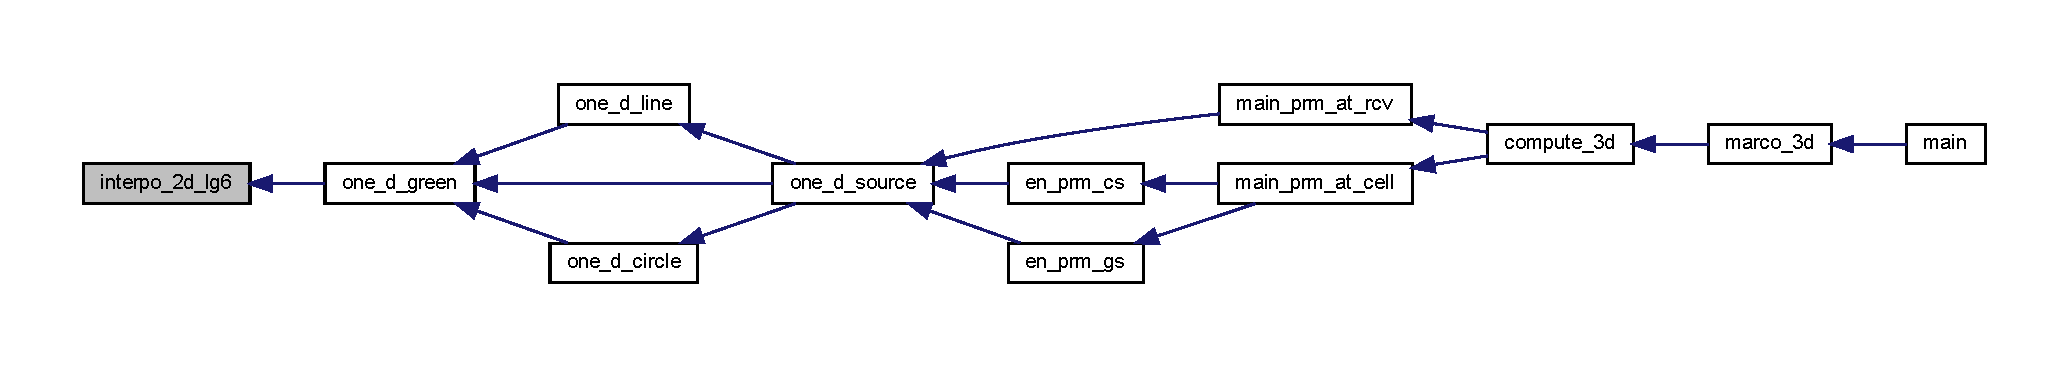
\includegraphics[width=350pt]{Marco_8f90_a170a0edeb8c14a416b4ec927bd0b5761_icgraph}
\end{center}
\end{figure}
\mbox{\Hypertarget{Marco_8f90_ab4eafb4c3c596148d85f446d1eb69d54}\label{Marco_8f90_ab4eafb4c3c596148d85f446d1eb69d54}} 
\index{Marco.\+f90@{Marco.\+f90}!interpo\+\_\+lg@{interpo\+\_\+lg}}
\index{interpo\+\_\+lg@{interpo\+\_\+lg}!Marco.\+f90@{Marco.\+f90}}
\subsubsection{\texorpdfstring{interpo\+\_\+lg()}{interpo\_lg()}}
{\footnotesize\ttfamily subroutine interpo\+\_\+lg (\begin{DoxyParamCaption}\item[{complex, dimension(11,nhfilm,nzsr,nzob)}]{G\+R\+HF,  }\item[{real, dimension(l)}]{A,  }\item[{integer}]{L,  }\item[{integer}]{N\+H\+F\+I\+LM,  }\item[{integer}]{N\+Z\+SR,  }\item[{integer}]{N\+Z\+OB,  }\item[{real}]{X,  }\item[{integer}]{I\+OB,  }\item[{integer}]{I\+SR,  }\item[{complex, dimension(nf)}]{F,  }\item[{integer}]{NF }\end{DoxyParamCaption})}

Here is the caller graph for this function\+:
\nopagebreak
\begin{figure}[H]
\begin{center}
\leavevmode
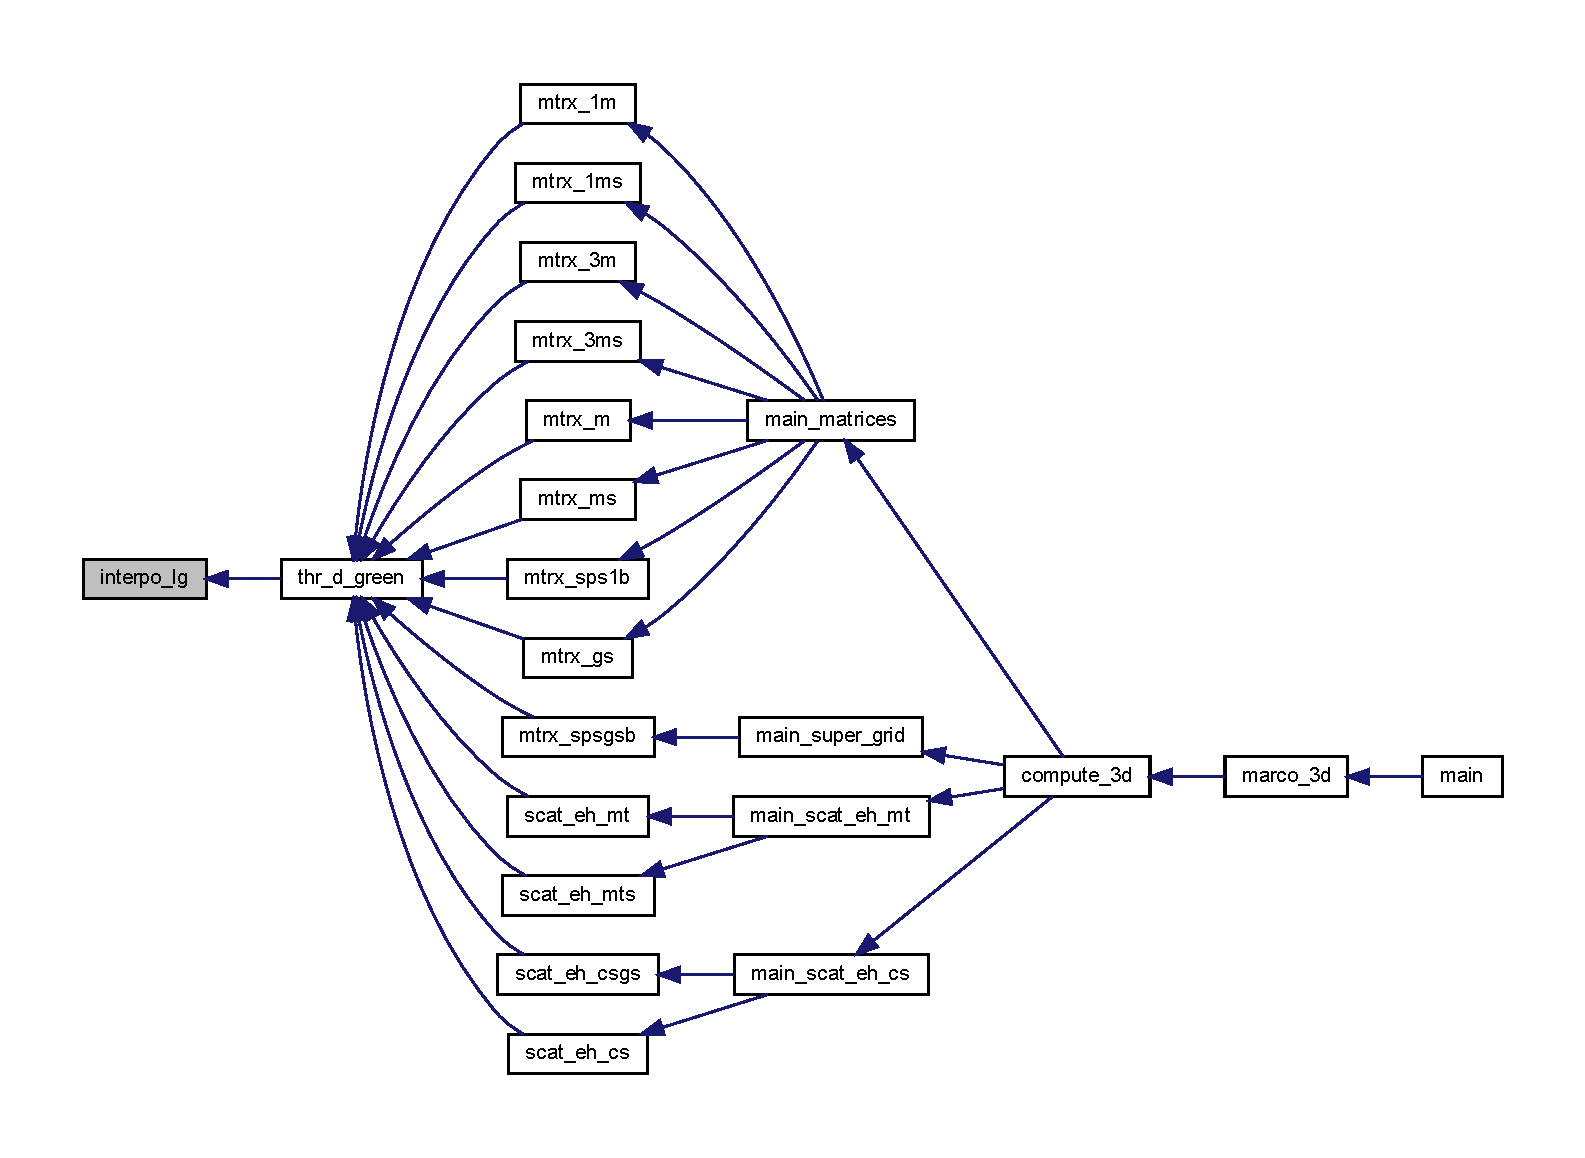
\includegraphics[width=350pt]{Marco_8f90_ab4eafb4c3c596148d85f446d1eb69d54_icgraph}
\end{center}
\end{figure}
\mbox{\Hypertarget{Marco_8f90_a3fe5c8bfe5e5729f1b02af3926c68dbc}\label{Marco_8f90_a3fe5c8bfe5e5729f1b02af3926c68dbc}} 
\index{Marco.\+f90@{Marco.\+f90}!interpo\+\_\+lg1@{interpo\+\_\+lg1}}
\index{interpo\+\_\+lg1@{interpo\+\_\+lg1}!Marco.\+f90@{Marco.\+f90}}
\subsubsection{\texorpdfstring{interpo\+\_\+lg1()}{interpo\_lg1()}}
{\footnotesize\ttfamily subroutine interpo\+\_\+lg1 (\begin{DoxyParamCaption}\item[{complex, dimension(11,nhfilm,nzsr)}]{G\+R\+H\+F3,  }\item[{real, dimension(l)}]{A,  }\item[{integer}]{L,  }\item[{integer}]{N\+H\+F\+I\+LM,  }\item[{integer}]{N\+Z\+SR,  }\item[{real}]{X,  }\item[{integer}]{I\+SR,  }\item[{complex, dimension(nf)}]{F,  }\item[{integer}]{NF }\end{DoxyParamCaption})}

Here is the caller graph for this function\+:
\nopagebreak
\begin{figure}[H]
\begin{center}
\leavevmode
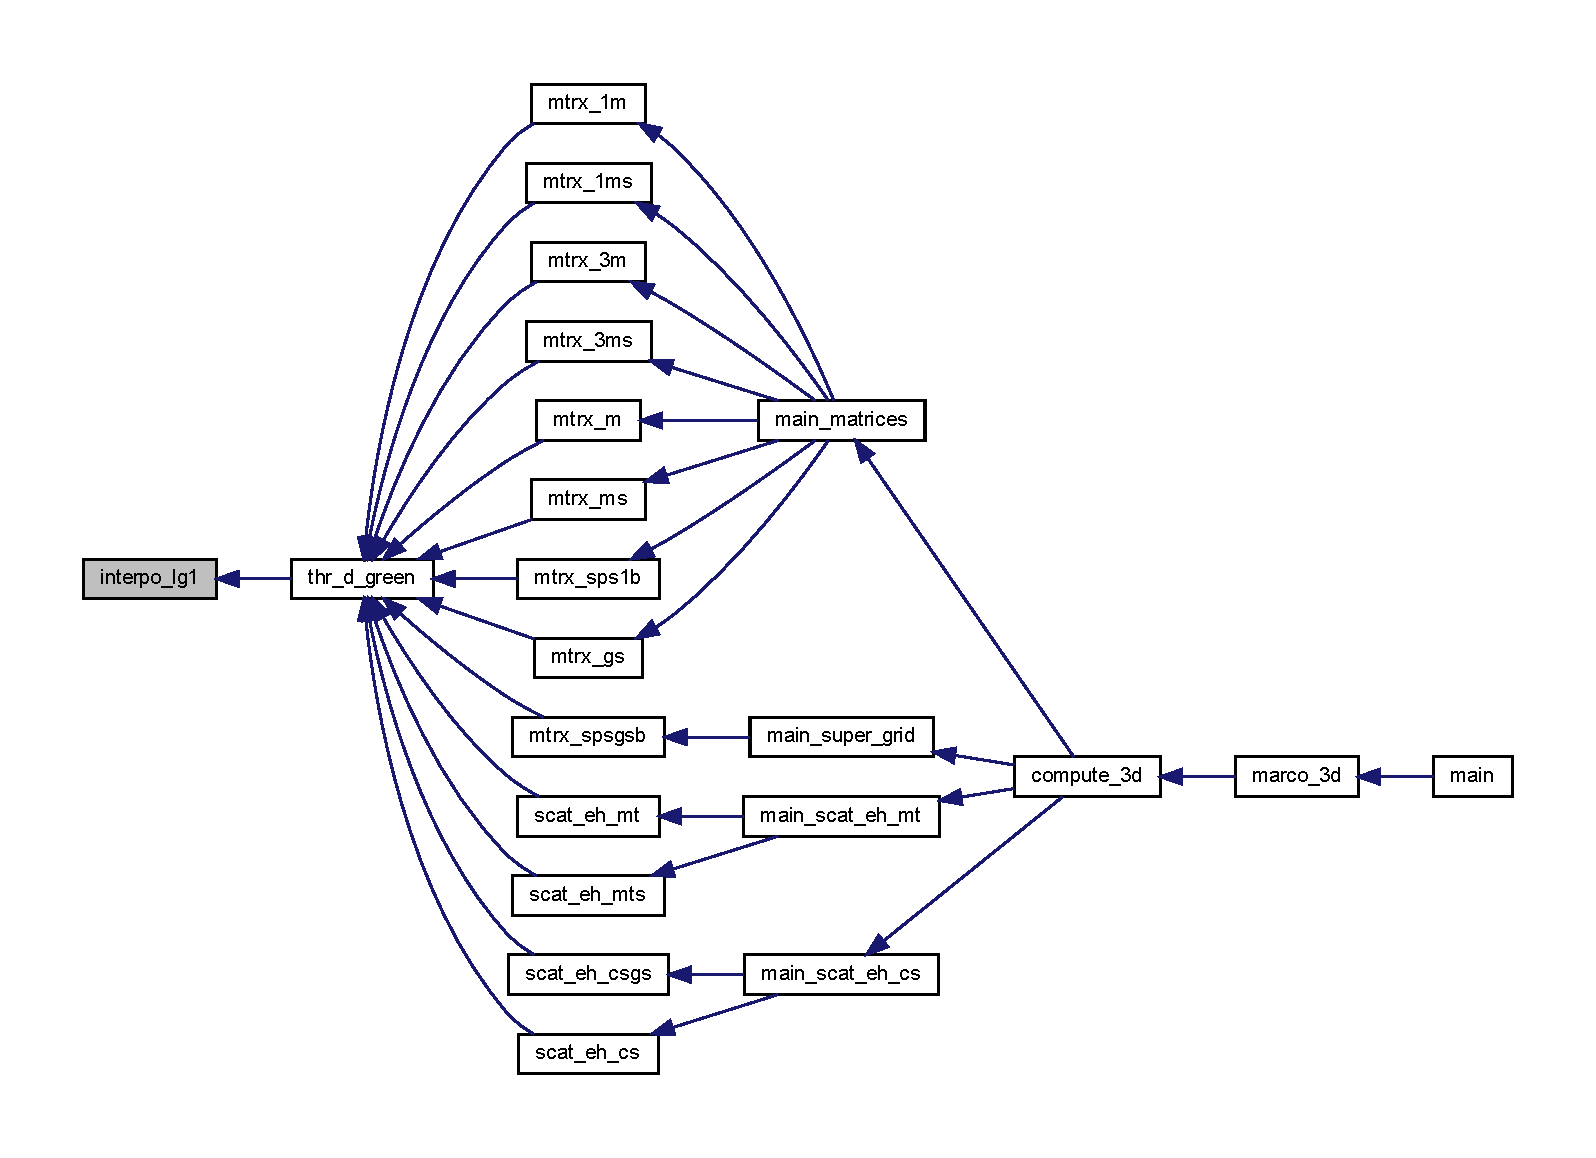
\includegraphics[width=350pt]{Marco_8f90_a3fe5c8bfe5e5729f1b02af3926c68dbc_icgraph}
\end{center}
\end{figure}
\mbox{\Hypertarget{Marco_8f90_a351cb438e704ef189fa972f9590cbd80}\label{Marco_8f90_a351cb438e704ef189fa972f9590cbd80}} 
\index{Marco.\+f90@{Marco.\+f90}!interpo\+\_\+lg4@{interpo\+\_\+lg4}}
\index{interpo\+\_\+lg4@{interpo\+\_\+lg4}!Marco.\+f90@{Marco.\+f90}}
\subsubsection{\texorpdfstring{interpo\+\_\+lg4()}{interpo\_lg4()}}
{\footnotesize\ttfamily subroutine interpo\+\_\+lg4 (\begin{DoxyParamCaption}\item[{complex, dimension(11,nhfilm,nzsr,nzob)}]{G\+R\+HF,  }\item[{real, dimension(l)}]{A,  }\item[{integer}]{L,  }\item[{integer}]{N\+H\+F\+I\+LM,  }\item[{integer}]{N\+Z\+SR,  }\item[{integer}]{N\+Z\+OB,  }\item[{real}]{X,  }\item[{integer}]{I\+OB,  }\item[{integer}]{I\+SR,  }\item[{complex, dimension(nf)}]{F,  }\item[{integer}]{NF }\end{DoxyParamCaption})}

Here is the caller graph for this function\+:
\nopagebreak
\begin{figure}[H]
\begin{center}
\leavevmode
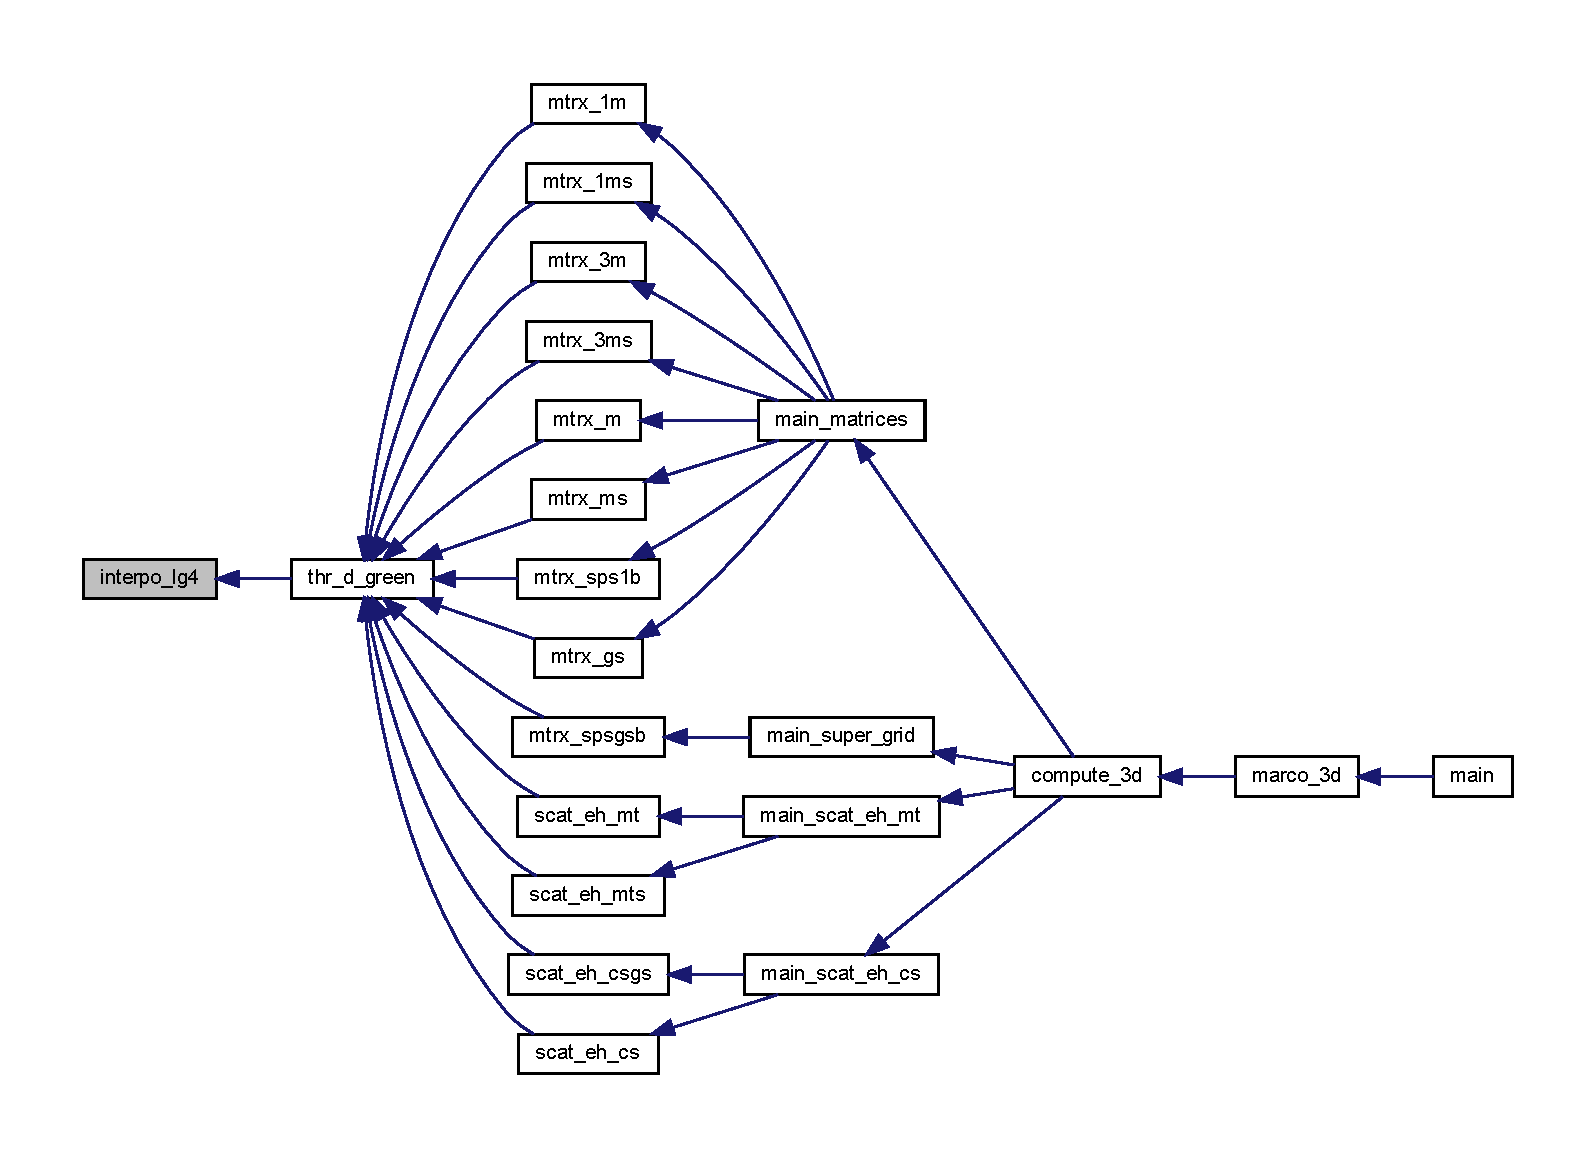
\includegraphics[width=350pt]{Marco_8f90_a351cb438e704ef189fa972f9590cbd80_icgraph}
\end{center}
\end{figure}
\mbox{\Hypertarget{Marco_8f90_a1715ef788d21f1b4a8008fdf5f53bfc2}\label{Marco_8f90_a1715ef788d21f1b4a8008fdf5f53bfc2}} 
\index{Marco.\+f90@{Marco.\+f90}!interpo\+\_\+lg5@{interpo\+\_\+lg5}}
\index{interpo\+\_\+lg5@{interpo\+\_\+lg5}!Marco.\+f90@{Marco.\+f90}}
\subsubsection{\texorpdfstring{interpo\+\_\+lg5()}{interpo\_lg5()}}
{\footnotesize\ttfamily subroutine interpo\+\_\+lg5 (\begin{DoxyParamCaption}\item[{complex, dimension(11,nhfilm,nzsr)}]{G\+R\+H\+F3,  }\item[{real, dimension(l)}]{A,  }\item[{integer}]{L,  }\item[{integer}]{N\+H\+F\+I\+LM,  }\item[{integer}]{N\+Z\+SR,  }\item[{real}]{X,  }\item[{integer}]{I\+SR,  }\item[{complex, dimension(nf)}]{F,  }\item[{integer}]{NF }\end{DoxyParamCaption})}

Here is the caller graph for this function\+:
\nopagebreak
\begin{figure}[H]
\begin{center}
\leavevmode
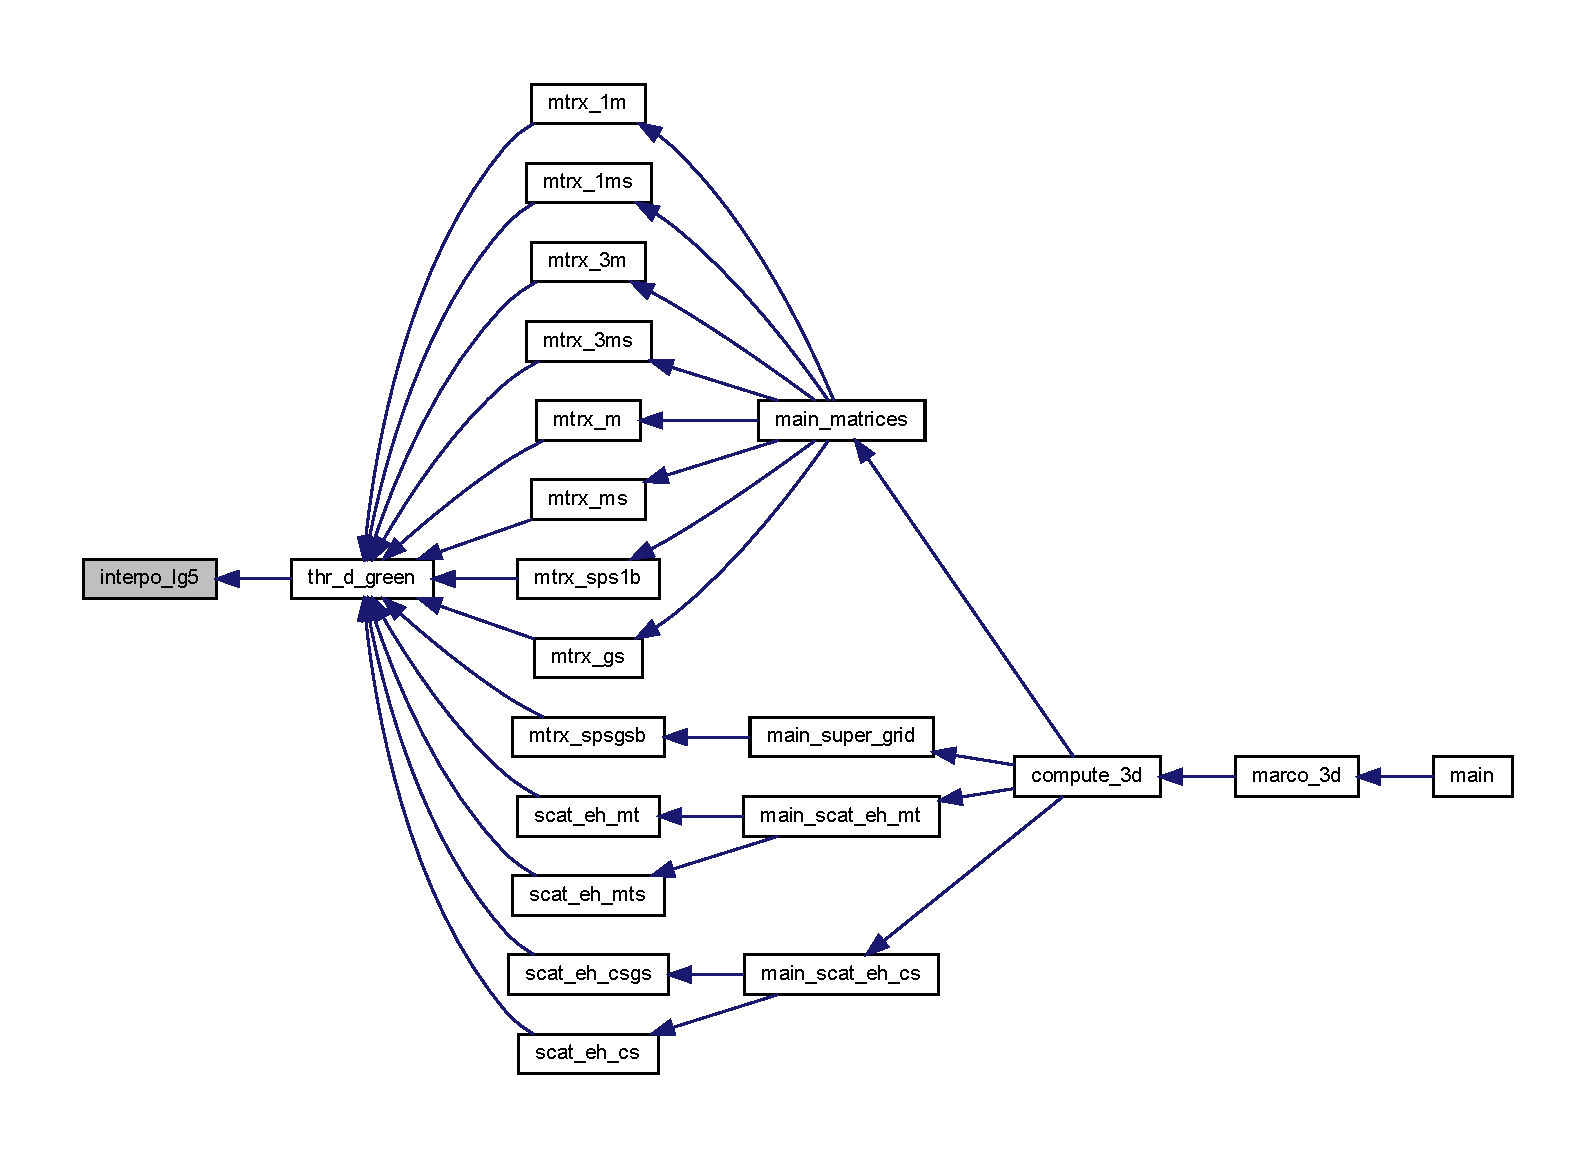
\includegraphics[width=350pt]{Marco_8f90_a1715ef788d21f1b4a8008fdf5f53bfc2_icgraph}
\end{center}
\end{figure}
\mbox{\Hypertarget{Marco_8f90_a5fa32081a6f961179118c3eed68de85f}\label{Marco_8f90_a5fa32081a6f961179118c3eed68de85f}} 
\index{Marco.\+f90@{Marco.\+f90}!interpo\+\_\+lg6@{interpo\+\_\+lg6}}
\index{interpo\+\_\+lg6@{interpo\+\_\+lg6}!Marco.\+f90@{Marco.\+f90}}
\subsubsection{\texorpdfstring{interpo\+\_\+lg6()}{interpo\_lg6()}}
{\footnotesize\ttfamily subroutine interpo\+\_\+lg6 (\begin{DoxyParamCaption}\item[{complex, dimension(11,nhfilm,nzsr,nzob)}]{G\+R\+HF,  }\item[{real, dimension(l)}]{A,  }\item[{integer}]{L,  }\item[{integer}]{N\+H\+F\+I\+LM,  }\item[{integer}]{N\+Z\+SR,  }\item[{integer}]{N\+Z\+OB,  }\item[{real}]{X,  }\item[{integer}]{I\+OB,  }\item[{integer}]{I\+SR,  }\item[{complex, dimension(nf)}]{F,  }\item[{integer}]{NF }\end{DoxyParamCaption})}

Here is the caller graph for this function\+:
\nopagebreak
\begin{figure}[H]
\begin{center}
\leavevmode
\includegraphics[width=350pt]{Marco_8f90_a5fa32081a6f961179118c3eed68de85f_icgraph}
\end{center}
\end{figure}
\mbox{\Hypertarget{Marco_8f90_a26481105d1de3f776fc36a094d319fbb}\label{Marco_8f90_a26481105d1de3f776fc36a094d319fbb}} 
\index{Marco.\+f90@{Marco.\+f90}!interpo\+\_\+lg6\+\_\+rho0@{interpo\+\_\+lg6\+\_\+rho0}}
\index{interpo\+\_\+lg6\+\_\+rho0@{interpo\+\_\+lg6\+\_\+rho0}!Marco.\+f90@{Marco.\+f90}}
\subsubsection{\texorpdfstring{interpo\+\_\+lg6\+\_\+rho0()}{interpo\_lg6\_rho0()}}
{\footnotesize\ttfamily subroutine interpo\+\_\+lg6\+\_\+rho0 (\begin{DoxyParamCaption}\item[{complex, dimension(4,nzsr,nzob)}]{G\+R\+H\+O0,  }\item[{integer}]{N\+Z\+SR,  }\item[{integer}]{N\+Z\+OB,  }\item[{integer}]{I\+OB,  }\item[{real}]{Z\+SR,  }\item[{real, dimension(2,nzsr)}]{Z\+S\+RG,  }\item[{complex, dimension(nf)}]{F,  }\item[{integer}]{NF }\end{DoxyParamCaption})}

Here is the caller graph for this function\+:
\nopagebreak
\begin{figure}[H]
\begin{center}
\leavevmode
\includegraphics[width=350pt]{Marco_8f90_a26481105d1de3f776fc36a094d319fbb_icgraph}
\end{center}
\end{figure}
\mbox{\Hypertarget{Marco_8f90_afd0f4c3b7f02fba61d9bd11b3a142ac2}\label{Marco_8f90_afd0f4c3b7f02fba61d9bd11b3a142ac2}} 
\index{Marco.\+f90@{Marco.\+f90}!interpo\+\_\+plpol@{interpo\+\_\+plpol}}
\index{interpo\+\_\+plpol@{interpo\+\_\+plpol}!Marco.\+f90@{Marco.\+f90}}
\subsubsection{\texorpdfstring{interpo\+\_\+plpol()}{interpo\_plpol()}}
{\footnotesize\ttfamily subroutine interpo\+\_\+plpol (\begin{DoxyParamCaption}\item[{complex, dimension(11,nhfilm,nzsr,nzob), intent(in)}]{G\+R\+HF,  }\item[{real, dimension(l), intent(in)}]{A,  }\item[{integer, intent(in)}]{L,  }\item[{integer, intent(in)}]{N\+H\+F\+I\+LM,  }\item[{integer, intent(in)}]{N\+Z\+SR,  }\item[{integer, intent(in)}]{N\+Z\+OB,  }\item[{real}]{X,  }\item[{integer, intent(in)}]{I\+OB,  }\item[{integer, intent(in)}]{I\+SR,  }\item[{complex, dimension(nf), intent(out)}]{F,  }\item[{integer, intent(in)}]{NF }\end{DoxyParamCaption})}

Here is the call graph for this function\+:
\nopagebreak
\begin{figure}[H]
\begin{center}
\leavevmode
\includegraphics[width=261pt]{Marco_8f90_afd0f4c3b7f02fba61d9bd11b3a142ac2_cgraph}
\end{center}
\end{figure}
Here is the caller graph for this function\+:
\nopagebreak
\begin{figure}[H]
\begin{center}
\leavevmode
\includegraphics[width=350pt]{Marco_8f90_afd0f4c3b7f02fba61d9bd11b3a142ac2_icgraph}
\end{center}
\end{figure}
\mbox{\Hypertarget{Marco_8f90_aadd0426cc10854791039735bfa14140d}\label{Marco_8f90_aadd0426cc10854791039735bfa14140d}} 
\index{Marco.\+f90@{Marco.\+f90}!interpo\+\_\+polint@{interpo\+\_\+polint}}
\index{interpo\+\_\+polint@{interpo\+\_\+polint}!Marco.\+f90@{Marco.\+f90}}
\subsubsection{\texorpdfstring{interpo\+\_\+polint()}{interpo\_polint()}}
{\footnotesize\ttfamily subroutine interpo\+\_\+polint (\begin{DoxyParamCaption}\item[{real, dimension(n)}]{XA,  }\item[{complex, dimension(n)}]{YA,  }\item[{integer}]{N,  }\item[{real}]{X,  }\item[{complex}]{Y,  }\item[{complex}]{DY }\end{DoxyParamCaption})}

Here is the caller graph for this function\+:
\nopagebreak
\begin{figure}[H]
\begin{center}
\leavevmode
\includegraphics[width=350pt]{Marco_8f90_aadd0426cc10854791039735bfa14140d_icgraph}
\end{center}
\end{figure}
\mbox{\Hypertarget{Marco_8f90_ab3d44a77ee1868f9a09dcac7e6bfcdce}\label{Marco_8f90_ab3d44a77ee1868f9a09dcac7e6bfcdce}} 
\index{Marco.\+f90@{Marco.\+f90}!interv@{interv}}
\index{interv@{interv}!Marco.\+f90@{Marco.\+f90}}
\subsubsection{\texorpdfstring{interv()}{interv()}}
{\footnotesize\ttfamily subroutine interv (\begin{DoxyParamCaption}\item[{real, dimension(lxt)}]{XT,  }\item[{integer}]{L\+XT,  }\item[{real}]{X,  }\item[{integer}]{L\+E\+FT,  }\item[{integer}]{M\+F\+L\+AG }\end{DoxyParamCaption})}

Here is the caller graph for this function\+:
\nopagebreak
\begin{figure}[H]
\begin{center}
\leavevmode
\includegraphics[width=202pt]{Marco_8f90_ab3d44a77ee1868f9a09dcac7e6bfcdce_icgraph}
\end{center}
\end{figure}
\mbox{\Hypertarget{Marco_8f90_a16c36ed9a25ca6e68931c4a00d2778e5}\label{Marco_8f90_a16c36ed9a25ca6e68931c4a00d2778e5}} 
\index{Marco.\+f90@{Marco.\+f90}!isamax@{isamax}}
\index{isamax@{isamax}!Marco.\+f90@{Marco.\+f90}}
\subsubsection{\texorpdfstring{isamax()}{isamax()}}
{\footnotesize\ttfamily integer function isamax (\begin{DoxyParamCaption}\item[{integer}]{N,  }\item[{complex, dimension(n)}]{SX,  }\item[{integer}]{I\+N\+CX }\end{DoxyParamCaption})}

\mbox{\Hypertarget{Marco_8f90_accb3ec8ce6fe855a60b0c1959fc6e2c8}\label{Marco_8f90_accb3ec8ce6fe855a60b0c1959fc6e2c8}} 
\index{Marco.\+f90@{Marco.\+f90}!linval@{linval}}
\index{linval@{linval}!Marco.\+f90@{Marco.\+f90}}
\subsubsection{\texorpdfstring{linval()}{linval()}}
{\footnotesize\ttfamily real function linval (\begin{DoxyParamCaption}\item[{integer, intent(in)}]{NX,  }\item[{real, dimension(nx), intent(in)}]{X\+V\+AL,  }\item[{real, dimension(nx,3), intent(in)}]{Y\+V\+AL,  }\item[{integer}]{K1,  }\item[{real, intent(in)}]{X1 }\end{DoxyParamCaption})}

Here is the call graph for this function\+:
\nopagebreak
\begin{figure}[H]
\begin{center}
\leavevmode
\includegraphics[width=196pt]{Marco_8f90_accb3ec8ce6fe855a60b0c1959fc6e2c8_cgraph}
\end{center}
\end{figure}
\mbox{\Hypertarget{Marco_8f90_acbb31184506555aa865f529467a59933}\label{Marco_8f90_acbb31184506555aa865f529467a59933}} 
\index{Marco.\+f90@{Marco.\+f90}!lp\+\_\+vertex\+\_\+order@{lp\+\_\+vertex\+\_\+order}}
\index{lp\+\_\+vertex\+\_\+order@{lp\+\_\+vertex\+\_\+order}!Marco.\+f90@{Marco.\+f90}}
\subsubsection{\texorpdfstring{lp\+\_\+vertex\+\_\+order()}{lp\_vertex\_order()}}
{\footnotesize\ttfamily subroutine lp\+\_\+vertex\+\_\+order (\begin{DoxyParamCaption}\item[{integer}]{N\+T\+XE,  }\item[{integer}]{M\+X\+V\+R\+TX,  }\item[{integer, dimension(ntxe)}]{N\+\_\+\+V\+R\+TX,  }\item[{real, dimension (mxvrtx,ntxe)}]{S\+XN,  }\item[{real, dimension (mxvrtx,ntxe)}]{S\+XE,  }\item[{real, dimension (mxvrtx,ntxe)}]{S\+XZ }\end{DoxyParamCaption})}

Here is the caller graph for this function\+:
\nopagebreak
\begin{figure}[H]
\begin{center}
\leavevmode
\includegraphics[width=237pt]{Marco_8f90_acbb31184506555aa865f529467a59933_icgraph}
\end{center}
\end{figure}
\mbox{\Hypertarget{Marco_8f90_a8ec2266d83cd6c0b762cbcbc92c0af3d}\label{Marco_8f90_a8ec2266d83cd6c0b762cbcbc92c0af3d}} 
\index{Marco.\+f90@{Marco.\+f90}!main@{main}}
\index{main@{main}!Marco.\+f90@{Marco.\+f90}}
\subsubsection{\texorpdfstring{main()}{main()}}
{\footnotesize\ttfamily program main (\begin{DoxyParamCaption}{ }\end{DoxyParamCaption})}

Here is the call graph for this function\+:
\nopagebreak
\begin{figure}[H]
\begin{center}
\leavevmode
\includegraphics[height=550pt]{Marco_8f90_a8ec2266d83cd6c0b762cbcbc92c0af3d_cgraph}
\end{center}
\end{figure}
\mbox{\Hypertarget{Marco_8f90_a399bcda7d08fa780bc7a58673659436b}\label{Marco_8f90_a399bcda7d08fa780bc7a58673659436b}} 
\index{Marco.\+f90@{Marco.\+f90}!main\+\_\+matrices@{main\+\_\+matrices}}
\index{main\+\_\+matrices@{main\+\_\+matrices}!Marco.\+f90@{Marco.\+f90}}
\subsubsection{\texorpdfstring{main\+\_\+matrices()}{main\_matrices()}}
{\footnotesize\ttfamily subroutine main\+\_\+matrices (\begin{DoxyParamCaption}\item[{integer}]{NW,  }\item[{integer}]{H\+I\+G\+H\+\_\+\+F\+RQ,  }\item[{integer}]{N\+P\+OL,  }\item[{integer}]{K\+S\+MR,  }\item[{real, dimension(nbody)}]{C\+L\+MN,  }\item[{integer}]{K\+A\+N\+IS,  }\item[{integer}]{K\+B\+O\+U\+ND,  }\item[{integer}]{K\+S\+Y\+MM,  }\item[{integer}]{C\+S\+\_\+\+T\+Y\+PE,  }\item[{integer}]{K\+C\+O\+ND,  }\item[{complex, dimension(nmax,nmax)}]{GA,  }\item[{complex, dimension(nsmr/3,3)}]{G\+S\+B2,  }\item[{integer, dimension(nmax)}]{I\+ND,  }\item[{real, dimension(nmax)}]{VV,  }\item[{real, dimension(nmax)}]{G\+AI,  }\item[{complex, dimension(nmax)}]{EN,  }\item[{complex, dimension(nmax)}]{E\+MT,  }\item[{complex, dimension(nsubcm,nbmax)}]{C\+DB,  }\item[{integer}]{M\+B\+O\+DY,  }\item[{integer}]{N\+B\+M\+AX,  }\item[{integer}]{N\+X\+M\+AX,  }\item[{integer}]{N\+Y\+M\+AX,  }\item[{integer}]{N\+Z\+M\+AX,  }\item[{integer}]{N\+S\+U\+B\+CM,  }\item[{integer}]{N\+B\+O\+DY,  }\item[{integer, dimension(mbody)}]{S\+U\+B\+\_\+\+B\+L\+O\+CK,  }\item[{integer, dimension(mbody)}]{N\+ET,  }\item[{integer, dimension(nbmax,mbody)}]{NX,  }\item[{integer, dimension(nbmax,mbody)}]{NY,  }\item[{integer, dimension(nbmax,mbody)}]{NZ,  }\item[{integer, dimension(nbmax,mbody)}]{N\+C\+E\+LL,  }\item[{real, dimension(nbmax,mbody)}]{B\+LX,  }\item[{real, dimension(nbmax,mbody)}]{B\+LY,  }\item[{real, dimension(nbmax,mbody)}]{B\+LZ,  }\item[{real, dimension(nxmax,nbmax,mbody)}]{X\+C\+E\+LL,  }\item[{real, dimension(nymax,nbmax,mbody)}]{Y\+C\+E\+LL,  }\item[{real, dimension(nzmax,nbmax,mbody)}]{Z\+C\+E\+LL,  }\item[{integer, dimension(mbody)}]{K\+C\+E\+LL,  }\item[{integer}]{N\+EQ,  }\item[{integer}]{N\+M\+AX,  }\item[{integer, dimension(nbmax)}]{N\+XI,  }\item[{integer, dimension(nbmax)}]{N\+YI,  }\item[{integer, dimension(nbmax)}]{N\+ZI,  }\item[{integer, dimension(nbmax)}]{N\+C\+E\+L\+LI,  }\item[{real, dimension(nbmax)}]{B\+L\+XI,  }\item[{real, dimension(nbmax)}]{B\+L\+YI,  }\item[{real, dimension(nbmax)}]{B\+L\+ZI,  }\item[{real, dimension(nxmax,nbmax)}]{X\+C\+E\+L\+LI,  }\item[{real, dimension(nymax,nbmax)}]{Y\+C\+E\+L\+LI,  }\item[{real, dimension(nzmax,nbmax)}]{Z\+C\+E\+L\+LI,  }\item[{integer, dimension(nbmax)}]{N\+XJ,  }\item[{integer, dimension(nbmax)}]{N\+YJ,  }\item[{integer, dimension(nbmax)}]{N\+ZJ,  }\item[{integer, dimension(nbmax)}]{N\+C\+E\+L\+LJ,  }\item[{real, dimension(nxmax,nbmax)}]{X\+C\+E\+L\+LJ,  }\item[{real, dimension(nymax,nbmax)}]{Y\+C\+E\+L\+LJ,  }\item[{real, dimension(nzmax,nbmax)}]{Z\+C\+E\+L\+LJ,  }\item[{real}]{S\+BX,  }\item[{real}]{S\+BY,  }\item[{real}]{S\+BZ,  }\item[{integer}]{N\+XS,  }\item[{integer}]{N\+YS,  }\item[{integer}]{N\+ZS,  }\item[{real}]{Z\+SB,  }\item[{integer}]{N\+S\+MR,  }\item[{real}]{F\+RQ,  }\item[{integer}]{M\+L\+A\+Y\+ER,  }\item[{real, dimension(0\+:mlayer)}]{Z\+B\+ND,  }\item[{real, dimension(mlayer)}]{L\+R\+Y\+TH,  }\item[{complex, dimension(0\+:mlayer)}]{K\+KH,  }\item[{complex, dimension(0\+:mlayer)}]{C\+DH,  }\item[{complex, dimension(0\+:mlayer)}]{C\+DV,  }\item[{real, dimension(0\+:mlayer)}]{H\+VK,  }\item[{integer}]{N\+Z\+OB,  }\item[{real, dimension(nzob)}]{Z\+O\+BG,  }\item[{integer}]{N\+Z\+SR,  }\item[{real, dimension(2,nzsr)}]{Z\+S\+RG,  }\item[{real}]{D\+M\+IN,  }\item[{integer}]{N\+H\+F\+I\+LM,  }\item[{real}]{R\+H\+O\+M\+IN,  }\item[{real}]{R\+H\+O\+M\+AX,  }\item[{real, dimension(nhfilm)}]{R\+RG,  }\item[{real, dimension(nhfilm)}]{R\+R\+G3,  }\item[{complex, dimension(11,nhfilm,nzsr,nzob)}]{G\+R\+HF,  }\item[{complex, dimension(11,nhfilm,nzsr)}]{G\+R\+H\+F3,  }\item[{complex, dimension(4,nzsr,nzob)}]{G\+R\+H\+O0,  }\item[{complex, dimension(4,nzsr)}]{G\+R\+H\+O03,  }\item[{real}]{A\+L\+M\+AX,  }\item[{integer}]{K\+S\+FT,  }\item[{integer}]{K\+C\+L\+MN,  }\item[{real}]{B\+L\+M\+IN,  }\item[{integer}]{K\+A\+CC,  }\item[{integer}]{K\+U\+T\+C\+RP }\end{DoxyParamCaption})}

Here is the call graph for this function\+:
\nopagebreak
\begin{figure}[H]
\begin{center}
\leavevmode
\includegraphics[width=350pt]{Marco_8f90_a399bcda7d08fa780bc7a58673659436b_cgraph}
\end{center}
\end{figure}
Here is the caller graph for this function\+:
\nopagebreak
\begin{figure}[H]
\begin{center}
\leavevmode
\includegraphics[width=350pt]{Marco_8f90_a399bcda7d08fa780bc7a58673659436b_icgraph}
\end{center}
\end{figure}
\mbox{\Hypertarget{Marco_8f90_a81389ef2893dbfd5d6a4c769758b1336}\label{Marco_8f90_a81389ef2893dbfd5d6a4c769758b1336}} 
\index{Marco.\+f90@{Marco.\+f90}!main\+\_\+prm\+\_\+at\+\_\+cell@{main\+\_\+prm\+\_\+at\+\_\+cell}}
\index{main\+\_\+prm\+\_\+at\+\_\+cell@{main\+\_\+prm\+\_\+at\+\_\+cell}!Marco.\+f90@{Marco.\+f90}}
\subsubsection{\texorpdfstring{main\+\_\+prm\+\_\+at\+\_\+cell()}{main\_prm\_at\_cell()}}
{\footnotesize\ttfamily subroutine main\+\_\+prm\+\_\+at\+\_\+cell (\begin{DoxyParamCaption}\item[{integer}]{NW,  }\item[{real}]{F\+RQ,  }\item[{integer}]{M\+L\+A\+Y\+ER,  }\item[{real, dimension(0\+:mlayer)}]{Z\+B\+ND,  }\item[{real, dimension(mlayer)}]{L\+R\+Y\+TH,  }\item[{real, dimension(0\+:mlayer)}]{H\+VK,  }\item[{complex, dimension(0\+:mlayer)}]{K\+KH,  }\item[{complex, dimension(0\+:mlayer)}]{C\+DH,  }\item[{integer}]{K\+A\+N\+IS,  }\item[{integer}]{H\+I\+G\+H\+\_\+\+F\+RQ,  }\item[{integer}]{C\+S\+\_\+\+T\+Y\+PE,  }\item[{integer}]{K\+S\+Y\+MM,  }\item[{integer}]{M\+B\+O\+DY,  }\item[{integer}]{N\+B\+M\+AX,  }\item[{integer}]{N\+S\+U\+B\+CM,  }\item[{integer}]{N\+M\+AX,  }\item[{integer}]{N\+X\+M\+AX,  }\item[{integer}]{N\+Y\+M\+AX,  }\item[{integer}]{N\+Z\+M\+AX,  }\item[{integer}]{N\+T\+XE,  }\item[{real, dimension(2,ntxe)}]{M\+D\+\_\+\+A\+N\+G\+LE,  }\item[{integer}]{N\+C\+RD,  }\item[{integer, dimension(ntxe)}]{N\+\_\+\+V\+R\+TX,  }\item[{real, dimension(ncrd,ntxe)}]{T\+X\+\_\+\+C\+R\+DX,  }\item[{real, dimension(ncrd,ntxe)}]{T\+X\+\_\+\+C\+R\+DY,  }\item[{real, dimension(ncrd,ntxe)}]{T\+X\+\_\+\+C\+R\+DZ,  }\item[{real, dimension(ntxe)}]{R\+AD,  }\item[{integer}]{N\+P\+OL,  }\item[{integer}]{L\+P1,  }\item[{integer}]{L\+P2,  }\item[{integer}]{N\+B\+O\+DY,  }\item[{integer, dimension(mbody)}]{S\+U\+B\+\_\+\+B\+L\+O\+CK,  }\item[{integer, dimension(mbody)}]{N\+ET,  }\item[{integer}]{N\+EQ,  }\item[{integer, dimension(nbmax,mbody)}]{NX,  }\item[{integer, dimension(nbmax,mbody)}]{NY,  }\item[{integer, dimension(nbmax,mbody)}]{NZ,  }\item[{integer, dimension(nbmax,mbody)}]{N\+C\+E\+LL,  }\item[{real, dimension(nxmax,nbmax,mbody)}]{X\+C\+E\+LL,  }\item[{real, dimension(nymax,nbmax,mbody)}]{Y\+C\+E\+LL,  }\item[{real, dimension(nzmax,nbmax,mbody)}]{Z\+C\+E\+LL,  }\item[{integer, dimension(nbmax)}]{N\+XI,  }\item[{integer, dimension(nbmax)}]{N\+YI,  }\item[{integer, dimension(nbmax)}]{N\+ZI,  }\item[{integer, dimension(nbmax)}]{N\+C\+E\+L\+LI,  }\item[{real, dimension(nxmax,nbmax)}]{X\+C\+E\+L\+LI,  }\item[{real, dimension(nymax,nbmax)}]{Y\+C\+E\+L\+LI,  }\item[{real, dimension(nzmax,nbmax)}]{Z\+C\+E\+L\+LI,  }\item[{complex, dimension(nsubcm,nbmax)}]{C\+DB,  }\item[{complex, dimension(nmax)}]{EN,  }\item[{complex, dimension(nmax)}]{E\+MT,  }\item[{complex, dimension(nmax,nbody)}]{E\+NT,  }\item[{complex, dimension(4$\ast$nmax$\ast$mbody)}]{E\+J\+GS,  }\item[{complex, dimension(4$\ast$nmax$\ast$mbody)}]{E\+J\+G\+S2,  }\item[{real}]{R\+H\+O\+M\+IN,  }\item[{real}]{R\+H\+O\+M\+AX,  }\item[{integer}]{N\+Z\+OB,  }\item[{real, dimension(nzob)}]{Z\+O\+BG,  }\item[{integer}]{N\+Z\+SR,  }\item[{real, dimension(2,nzsr)}]{Z\+S\+RG,  }\item[{integer}]{N\+Z\+BG,  }\item[{real, dimension(2,nzbg)}]{Z\+BG,  }\item[{integer}]{K\+A\+CC,  }\item[{real}]{AJ,  }\item[{real}]{D\+M\+IN,  }\item[{integer}]{N\+H\+F\+I\+LM,  }\item[{real}]{A\+L\+M\+AX,  }\item[{real}]{B\+L\+M\+IN,  }\item[{complex, dimension(11,nhfilm,nzsr,nzob)}]{G\+R\+HF,  }\item[{real, dimension(nhfilm)}]{R\+RG,  }\item[{complex, dimension(4,nzsr,nzob)}]{G\+R\+H\+O0 }\end{DoxyParamCaption})}

Here is the call graph for this function\+:
\nopagebreak
\begin{figure}[H]
\begin{center}
\leavevmode
\includegraphics[width=350pt]{Marco_8f90_a81389ef2893dbfd5d6a4c769758b1336_cgraph}
\end{center}
\end{figure}
Here is the caller graph for this function\+:
\nopagebreak
\begin{figure}[H]
\begin{center}
\leavevmode
\includegraphics[width=350pt]{Marco_8f90_a81389ef2893dbfd5d6a4c769758b1336_icgraph}
\end{center}
\end{figure}
\mbox{\Hypertarget{Marco_8f90_adfc6a7cb71bd4ea9c02eaafd4d9e5664}\label{Marco_8f90_adfc6a7cb71bd4ea9c02eaafd4d9e5664}} 
\index{Marco.\+f90@{Marco.\+f90}!main\+\_\+prm\+\_\+at\+\_\+rcv@{main\+\_\+prm\+\_\+at\+\_\+rcv}}
\index{main\+\_\+prm\+\_\+at\+\_\+rcv@{main\+\_\+prm\+\_\+at\+\_\+rcv}!Marco.\+f90@{Marco.\+f90}}
\subsubsection{\texorpdfstring{main\+\_\+prm\+\_\+at\+\_\+rcv()}{main\_prm\_at\_rcv()}}
{\footnotesize\ttfamily subroutine main\+\_\+prm\+\_\+at\+\_\+rcv (\begin{DoxyParamCaption}\item[{integer, intent(in)}]{H\+I\+G\+H\+\_\+\+F\+RQ,  }\item[{integer}]{C\+S\+\_\+\+T\+Y\+PE,  }\item[{integer}]{K\+A\+CC,  }\item[{integer}]{M\+L\+A\+Y\+ER,  }\item[{real, dimension(0\+:mlayer), intent(in)}]{Z\+B\+ND,  }\item[{real, dimension(mlayer), intent(in)}]{R\+M\+U\+\_\+\+L\+YR,  }\item[{complex, dimension(0\+:mlayer)}]{C\+DH,  }\item[{real}]{F\+RQ,  }\item[{integer, intent(in)}]{N\+T\+XE,  }\item[{real, dimension(2,ntxe), intent(in)}]{M\+D\+\_\+\+A\+N\+G\+LE,  }\item[{integer, intent(in)}]{N\+C\+RD,  }\item[{integer, intent(in)}]{M\+\_\+\+RX,  }\item[{integer, dimension(m\+\_\+rx,ntxe), intent(in)}]{N\+\_\+\+S\+U\+B\+\_\+\+RX,  }\item[{integer, dimension(m\+\_\+rx,ntxe), intent(in)}]{R\+X\+\_\+\+T\+Y\+P\+E\+\_\+\+I\+N\+D\+EX,  }\item[{integer, intent(in)}]{S\+U\+B\+\_\+\+R\+X\+\_\+\+M\+AX,  }\item[{integer, intent(in)}]{S\+O\+U\+R\+C\+E\+\_\+\+T\+Y\+PE,  }\item[{integer, dimension(ntxe), intent(in)}]{N\+\_\+\+RX,  }\item[{real, dimension(sub\+\_\+rx\+\_\+max,m\+\_\+rx,ntxe), intent(in)}]{R\+X\+\_\+X,  }\item[{real, dimension(sub\+\_\+rx\+\_\+max,m\+\_\+rx,ntxe), intent(in)}]{R\+X\+\_\+Y,  }\item[{real, dimension(sub\+\_\+rx\+\_\+max,m\+\_\+rx,ntxe), intent(in)}]{R\+X\+\_\+Z,  }\item[{real, dimension(3,sub\+\_\+rx\+\_\+max,m\+\_\+rx,ntxe), intent(in)}]{R\+X\+\_\+\+W\+E\+I\+G\+HT,  }\item[{integer, dimension(ntxe), intent(in)}]{N\+\_\+\+V\+R\+TX,  }\item[{real, dimension(ncrd,ntxe), intent(in)}]{T\+X\+\_\+\+C\+R\+DX,  }\item[{real, dimension(ncrd,ntxe), intent(in)}]{T\+X\+\_\+\+C\+R\+DY,  }\item[{real, dimension(ncrd,ntxe), intent(in)}]{T\+X\+\_\+\+C\+R\+DZ,  }\item[{integer, intent(in)}]{E\+\_\+\+O\+N\+LY,  }\item[{complex, dimension(m\+\_\+rx,ntxe)}]{E\+NX,  }\item[{complex, dimension(m\+\_\+rx,ntxe)}]{E\+NY,  }\item[{complex, dimension(m\+\_\+rx,ntxe)}]{E\+NZ,  }\item[{complex, dimension(m\+\_\+rx,ntxe)}]{H\+NX,  }\item[{complex, dimension(m\+\_\+rx,ntxe)}]{H\+NY,  }\item[{complex, dimension(m\+\_\+rx,ntxe)}]{H\+NZ,  }\item[{complex, dimension(m\+\_\+rx,ntxe)}]{V\+L\+T1D,  }\item[{integer, intent(in)}]{N\+H\+F\+I\+LM,  }\item[{real, dimension(mlayer), intent(in)}]{L\+R\+Y\+TH,  }\item[{real, dimension(0\+:mlayer), intent(in)}]{H\+VK,  }\item[{complex, dimension(0\+:mlayer)}]{K\+KH,  }\item[{integer}]{K\+A\+N\+IS,  }\item[{real}]{B\+L\+M\+IN,  }\item[{real}]{D\+M\+IN,  }\item[{real}]{R\+H\+O\+M\+IN,  }\item[{real}]{R\+H\+O\+M\+AX,  }\item[{integer, intent(in)}]{N\+Z\+OB,  }\item[{real, dimension(nzob), intent(in)}]{Z\+O\+BG,  }\item[{integer, intent(in)}]{N\+Z\+SR,  }\item[{real, dimension(2,nzsr), intent(in)}]{Z\+S\+RG,  }\item[{integer, intent(in)}]{N\+Z\+BG,  }\item[{real, dimension(2,nzbg), intent(inout)}]{Z\+BG,  }\item[{real}]{A\+L\+M\+AX,  }\item[{complex, dimension(11,nhfilm,nzsr,nzob)}]{G\+R\+HF,  }\item[{real, dimension(nhfilm), intent(inout)}]{R\+RG,  }\item[{complex, dimension(4,nzsr,nzob)}]{G\+R\+H\+O0 }\end{DoxyParamCaption})}

Here is the call graph for this function\+:
\nopagebreak
\begin{figure}[H]
\begin{center}
\leavevmode
\includegraphics[width=350pt]{Marco_8f90_adfc6a7cb71bd4ea9c02eaafd4d9e5664_cgraph}
\end{center}
\end{figure}
Here is the caller graph for this function\+:
\nopagebreak
\begin{figure}[H]
\begin{center}
\leavevmode
\includegraphics[width=350pt]{Marco_8f90_adfc6a7cb71bd4ea9c02eaafd4d9e5664_icgraph}
\end{center}
\end{figure}
\mbox{\Hypertarget{Marco_8f90_a631581f8c126c181d87636784b2f6720}\label{Marco_8f90_a631581f8c126c181d87636784b2f6720}} 
\index{Marco.\+f90@{Marco.\+f90}!main\+\_\+scat\+\_\+eh\+\_\+cs@{main\+\_\+scat\+\_\+eh\+\_\+cs}}
\index{main\+\_\+scat\+\_\+eh\+\_\+cs@{main\+\_\+scat\+\_\+eh\+\_\+cs}!Marco.\+f90@{Marco.\+f90}}
\subsubsection{\texorpdfstring{main\+\_\+scat\+\_\+eh\+\_\+cs()}{main\_scat\_eh\_cs()}}
{\footnotesize\ttfamily subroutine main\+\_\+scat\+\_\+eh\+\_\+cs (\begin{DoxyParamCaption}\item[{integer, intent(in)}]{S\+U\+B\+\_\+\+R\+X\+\_\+\+M\+AX,  }\item[{integer, dimension(m\+\_\+rx,ntxe), intent(in)}]{R\+X\+\_\+\+T\+Y\+P\+E\+\_\+\+I\+N\+D\+EX,  }\item[{integer}]{H\+I\+G\+H\+\_\+\+F\+RQ,  }\item[{integer}]{K\+A\+CC,  }\item[{integer}]{K\+S\+Y\+MM,  }\item[{integer}]{M\+B\+O\+DY,  }\item[{integer}]{N\+B\+M\+AX,  }\item[{integer}]{N\+S\+U\+B\+CM,  }\item[{integer}]{N\+B\+O\+DY,  }\item[{integer, dimension(mbody)}]{S\+U\+B\+\_\+\+B\+L\+O\+CK,  }\item[{integer, dimension(nbmax,mbody)}]{N\+C\+E\+LL,  }\item[{integer, dimension(mbody)}]{N\+ET,  }\item[{complex, dimension(nsubcm,nbmax,mbody)}]{T\+C\+DB,  }\item[{complex, dimension(nmax)}]{E\+MT,  }\item[{complex, dimension(nmax,mbody)}]{J\+ST,  }\item[{complex, dimension(4$\ast$nmax$\ast$mbody)}]{E\+J\+GS,  }\item[{integer}]{N\+M\+AX,  }\item[{integer}]{N\+T\+XE,  }\item[{integer, dimension(ntxe)}]{N\+\_\+\+RX,  }\item[{integer, dimension(m\+\_\+rx,ntxe)}]{N\+\_\+\+S\+U\+B\+\_\+\+RX,  }\item[{real, dimension(3,sub\+\_\+rx\+\_\+max,m\+\_\+rx,ntxe), intent(in)}]{R\+X\+\_\+\+W\+E\+I\+G\+HT,  }\item[{integer}]{N\+H\+F\+I\+LM,  }\item[{real}]{F\+RQ,  }\item[{integer}]{M\+L\+A\+Y\+ER,  }\item[{real, dimension(0\+:mlayer)}]{Z\+B\+ND,  }\item[{real, dimension(mlayer)}]{L\+R\+Y\+TH,  }\item[{real, dimension(0\+:mlayer)}]{H\+VK,  }\item[{complex, dimension(0\+:mlayer)}]{K\+KH,  }\item[{real, dimension(mlayer)}]{R\+M\+U\+\_\+\+L\+YR,  }\item[{integer}]{K\+A\+N\+IS,  }\item[{real}]{B\+L\+M\+IN,  }\item[{real}]{D\+M\+IN,  }\item[{real}]{R\+H\+O\+M\+IN,  }\item[{real}]{R\+H\+O\+M\+AX,  }\item[{integer}]{N\+Z\+OB,  }\item[{real, dimension(nzob)}]{Z\+O\+BG,  }\item[{integer}]{N\+Z\+SR,  }\item[{real, dimension(2,nzsr)}]{Z\+S\+RG,  }\item[{real}]{A\+L\+M\+AX,  }\item[{real, dimension(nhfilm)}]{R\+RG,  }\item[{real, dimension(nhfilm)}]{R\+R\+G3,  }\item[{complex, dimension(11,nhfilm,nzsr,nzob)}]{G\+R\+HF,  }\item[{complex, dimension(11,nhfilm,nzsr)}]{G\+R\+H\+F3,  }\item[{complex, dimension(4,nzsr,nzob)}]{G\+R\+H\+O0,  }\item[{complex, dimension(4,nzsr)}]{G\+R\+H\+O03,  }\item[{real, dimension(sub\+\_\+rx\+\_\+max,m\+\_\+rx,ntxe), intent(in)}]{R\+X\+\_\+X,  }\item[{real, dimension(sub\+\_\+rx\+\_\+max,m\+\_\+rx,ntxe), intent(in)}]{R\+X\+\_\+Y,  }\item[{real, dimension(sub\+\_\+rx\+\_\+max,m\+\_\+rx,ntxe), intent(in)}]{R\+X\+\_\+Z,  }\item[{integer}]{N\+X\+M\+AX,  }\item[{integer}]{N\+Y\+M\+AX,  }\item[{integer}]{N\+Z\+M\+AX,  }\item[{integer}]{N\+EQ,  }\item[{integer, dimension(nbmax,mbody)}]{NX,  }\item[{integer, dimension(nbmax,mbody)}]{NY,  }\item[{integer, dimension(nbmax,mbody)}]{NZ,  }\item[{real, dimension(nxmax,nbmax,mbody)}]{X\+C\+E\+LL,  }\item[{real, dimension(nymax,nbmax,mbody)}]{Y\+C\+E\+LL,  }\item[{real, dimension(nzmax,nbmax,mbody)}]{Z\+C\+E\+LL,  }\item[{real, dimension(nbmax,mbody)}]{B\+LX,  }\item[{real, dimension(nbmax,mbody)}]{B\+LY,  }\item[{real, dimension(nbmax,mbody)}]{B\+LZ,  }\item[{complex, dimension(0\+:mlayer)}]{C\+DH,  }\item[{complex, dimension(0\+:mlayer)}]{C\+DV,  }\item[{integer}]{K\+S\+FT,  }\item[{real, dimension(nbody)}]{C\+L\+MN,  }\item[{integer}]{M\+\_\+\+RX,  }\item[{complex, dimension(m\+\_\+rx,ntxe)}]{E\+NX,  }\item[{complex, dimension(m\+\_\+rx,ntxe)}]{E\+NY,  }\item[{complex, dimension(m\+\_\+rx,ntxe)}]{E\+NZ,  }\item[{complex, dimension(m\+\_\+rx)}]{E\+AX,  }\item[{complex, dimension(m\+\_\+rx)}]{E\+AY,  }\item[{complex, dimension(m\+\_\+rx)}]{E\+AZ,  }\item[{complex, dimension(m\+\_\+rx)}]{H\+AX,  }\item[{complex, dimension(m\+\_\+rx)}]{H\+AY,  }\item[{complex, dimension(m\+\_\+rx)}]{H\+AZ,  }\item[{complex, dimension(m\+\_\+rx,ntxe), intent(out)}]{V\+L\+T3D,  }\item[{complex, dimension(m\+\_\+rx,ntxe)}]{E\+SX,  }\item[{complex, dimension(m\+\_\+rx,ntxe)}]{E\+SY,  }\item[{complex, dimension(m\+\_\+rx,ntxe)}]{E\+SZ,  }\item[{complex, dimension(m\+\_\+rx,ntxe)}]{H\+SX,  }\item[{complex, dimension(m\+\_\+rx,ntxe)}]{H\+SY,  }\item[{complex, dimension(m\+\_\+rx,ntxe)}]{H\+SZ }\end{DoxyParamCaption})}

Here is the call graph for this function\+:
\nopagebreak
\begin{figure}[H]
\begin{center}
\leavevmode
\includegraphics[width=350pt]{Marco_8f90_a631581f8c126c181d87636784b2f6720_cgraph}
\end{center}
\end{figure}
Here is the caller graph for this function\+:
\nopagebreak
\begin{figure}[H]
\begin{center}
\leavevmode
\includegraphics[width=350pt]{Marco_8f90_a631581f8c126c181d87636784b2f6720_icgraph}
\end{center}
\end{figure}
\mbox{\Hypertarget{Marco_8f90_a691701461b67027619c9ea8471ee24ea}\label{Marco_8f90_a691701461b67027619c9ea8471ee24ea}} 
\index{Marco.\+f90@{Marco.\+f90}!main\+\_\+scat\+\_\+eh\+\_\+mt@{main\+\_\+scat\+\_\+eh\+\_\+mt}}
\index{main\+\_\+scat\+\_\+eh\+\_\+mt@{main\+\_\+scat\+\_\+eh\+\_\+mt}!Marco.\+f90@{Marco.\+f90}}
\subsubsection{\texorpdfstring{main\+\_\+scat\+\_\+eh\+\_\+mt()}{main\_scat\_eh\_mt()}}
{\footnotesize\ttfamily subroutine main\+\_\+scat\+\_\+eh\+\_\+mt (\begin{DoxyParamCaption}\item[{integer}]{H\+I\+G\+H\+\_\+\+F\+RQ,  }\item[{integer}]{K\+A\+CC,  }\item[{integer}]{K\+S\+Y\+MM,  }\item[{integer}]{M\+B\+O\+DY,  }\item[{integer}]{N\+B\+M\+AX,  }\item[{integer}]{N\+S\+U\+B\+CM,  }\item[{integer}]{N\+B\+O\+DY,  }\item[{integer, dimension(mbody)}]{S\+U\+B\+\_\+\+B\+L\+O\+CK,  }\item[{integer, dimension(nbmax,mbody)}]{N\+C\+E\+LL,  }\item[{complex, dimension(nsubcm,nbmax,mbody)}]{T\+C\+DB,  }\item[{complex, dimension(nmax,mbody)}]{J\+ST,  }\item[{integer}]{N\+M\+AX,  }\item[{integer}]{N\+H\+F\+I\+LM,  }\item[{real}]{F\+RQ,  }\item[{integer}]{M\+L\+A\+Y\+ER,  }\item[{real, dimension(0\+:mlayer)}]{Z\+B\+ND,  }\item[{real, dimension(mlayer)}]{L\+R\+Y\+TH,  }\item[{real, dimension(0\+:mlayer)}]{H\+VK,  }\item[{complex, dimension(0\+:mlayer)}]{K\+KH,  }\item[{integer}]{K\+A\+N\+IS,  }\item[{real}]{B\+L\+M\+IN,  }\item[{real}]{D\+M\+IN,  }\item[{real}]{R\+H\+O\+M\+IN,  }\item[{real}]{R\+H\+O\+M\+AX,  }\item[{integer}]{N\+Z\+OB,  }\item[{real, dimension(nzob)}]{Z\+O\+BG,  }\item[{integer}]{N\+Z\+SR,  }\item[{real, dimension(2,nzsr)}]{Z\+S\+RG,  }\item[{real}]{A\+L\+M\+AX,  }\item[{real, dimension(nhfilm)}]{R\+RG,  }\item[{real, dimension(nhfilm)}]{R\+R\+G3,  }\item[{complex, dimension(11,nhfilm,nzsr,nzob)}]{G\+R\+HF,  }\item[{complex, dimension(11,nhfilm,nzsr)}]{G\+R\+H\+F3,  }\item[{complex, dimension(4,nzsr,nzob)}]{G\+R\+H\+O0,  }\item[{complex, dimension(4,nzsr)}]{G\+R\+H\+O03,  }\item[{integer}]{M\+T\+\_\+\+P\+R\+O\+FL,  }\item[{integer}]{M\+T\+\_\+\+S\+T\+A\+TN,  }\item[{real, dimension(mt\+\_\+profl)}]{X\+R\+MT,  }\item[{real, dimension(mt\+\_\+statn)}]{Y\+R\+MT,  }\item[{integer}]{N\+X\+M\+AX,  }\item[{integer}]{N\+Y\+M\+AX,  }\item[{integer}]{N\+Z\+M\+AX,  }\item[{integer, dimension(nbmax,mbody)}]{NX,  }\item[{integer, dimension(nbmax,mbody)}]{NY,  }\item[{integer, dimension(nbmax,mbody)}]{NZ,  }\item[{real, dimension(nxmax,nbmax,mbody)}]{X\+C\+E\+LL,  }\item[{real, dimension(nymax,nbmax,mbody)}]{Y\+C\+E\+LL,  }\item[{real, dimension(nzmax,nbmax,mbody)}]{Z\+C\+E\+LL,  }\item[{real, dimension(nbmax,mbody)}]{B\+LX,  }\item[{real, dimension(nbmax,mbody)}]{B\+LY,  }\item[{real, dimension(nbmax,mbody)}]{B\+LZ,  }\item[{complex, dimension(0\+:mlayer)}]{C\+DH,  }\item[{integer}]{N\+P\+OL,  }\item[{complex}]{E0\+X1,  }\item[{complex}]{E0\+Y1,  }\item[{real}]{Z\+MT,  }\item[{integer}]{K\+S\+FT,  }\item[{real, dimension(nbody)}]{C\+L\+MN,  }\item[{complex, dimension(mt\+\_\+profl,mt\+\_\+statn,2)}]{E\+X\+MT,  }\item[{complex, dimension(mt\+\_\+profl,mt\+\_\+statn,2)}]{E\+Y\+MT,  }\item[{complex, dimension(mt\+\_\+profl,mt\+\_\+statn,2)}]{H\+X\+MT,  }\item[{complex, dimension(mt\+\_\+profl,mt\+\_\+statn,2)}]{H\+Y\+MT,  }\item[{complex, dimension(mt\+\_\+profl,mt\+\_\+statn,2)}]{H\+Z\+MT }\end{DoxyParamCaption})}

Here is the call graph for this function\+:
\nopagebreak
\begin{figure}[H]
\begin{center}
\leavevmode
\includegraphics[width=350pt]{Marco_8f90_a691701461b67027619c9ea8471ee24ea_cgraph}
\end{center}
\end{figure}
Here is the caller graph for this function\+:
\nopagebreak
\begin{figure}[H]
\begin{center}
\leavevmode
\includegraphics[width=350pt]{Marco_8f90_a691701461b67027619c9ea8471ee24ea_icgraph}
\end{center}
\end{figure}
\mbox{\Hypertarget{Marco_8f90_a212d574f24aa10a6e92151f2b35d968e}\label{Marco_8f90_a212d574f24aa10a6e92151f2b35d968e}} 
\index{Marco.\+f90@{Marco.\+f90}!main\+\_\+solver@{main\+\_\+solver}}
\index{main\+\_\+solver@{main\+\_\+solver}!Marco.\+f90@{Marco.\+f90}}
\subsubsection{\texorpdfstring{main\+\_\+solver()}{main\_solver()}}
{\footnotesize\ttfamily subroutine main\+\_\+solver (\begin{DoxyParamCaption}\item[{integer}]{NW,  }\item[{complex, dimension(nmax,nmax)}]{GA,  }\item[{integer, dimension(nmax)}]{I\+ND,  }\item[{complex, dimension(nmax)}]{E\+MT,  }\item[{complex, dimension(nmax)}]{EN,  }\item[{complex, dimension(nmax,mbody)}]{E\+NT,  }\item[{integer, dimension(mbody)}]{N\+ET,  }\item[{complex, dimension(nmax,mbody)}]{J\+ST,  }\item[{complex, dimension(4$\ast$nmax$\ast$mbody)}]{E\+J\+GS,  }\item[{complex, dimension(4$\ast$nmax$\ast$mbody)}]{E\+J\+G\+S2,  }\item[{integer}]{K\+A\+CC,  }\item[{integer}]{K\+S\+MR,  }\item[{integer}]{K\+S\+Y\+MM,  }\item[{integer}]{C\+S\+\_\+\+T\+Y\+PE,  }\item[{integer}]{K\+A\+N\+IS,  }\item[{integer}]{K\+B\+O\+U\+ND,  }\item[{integer}]{N\+T\+XE,  }\item[{integer}]{L\+P1,  }\item[{integer}]{L\+P2,  }\item[{integer}]{N\+P\+OL,  }\item[{integer}]{M\+B\+O\+DY,  }\item[{integer}]{N\+B\+M\+AX,  }\item[{integer}]{N\+X\+M\+AX,  }\item[{integer}]{N\+Y\+M\+AX,  }\item[{integer}]{N\+Z\+M\+AX,  }\item[{integer}]{N\+M\+AX,  }\item[{integer}]{N\+B\+O\+DY,  }\item[{integer, dimension(mbody)}]{S\+U\+B\+\_\+\+B\+L\+O\+CK,  }\item[{integer, dimension(nbmax,mbody)}]{NX,  }\item[{integer, dimension(nbmax,mbody)}]{NY,  }\item[{integer, dimension(nbmax,mbody)}]{NZ,  }\item[{integer, dimension(nbmax,mbody)}]{N\+C\+E\+LL,  }\item[{integer, dimension(mbody)}]{N\+CT,  }\item[{integer, dimension(mbody)}]{K\+C\+E\+LL,  }\item[{real, dimension(nxmax,nbmax,mbody)}]{X\+C\+E\+LL,  }\item[{real, dimension(nymax,nbmax,mbody)}]{Y\+C\+E\+LL,  }\item[{real, dimension(nzmax,nbmax,mbody)}]{Z\+C\+E\+LL,  }\item[{real, dimension(nbmax,mbody)}]{B\+LX,  }\item[{real, dimension(nbmax,mbody)}]{B\+LY,  }\item[{real, dimension(nbmax,mbody)}]{B\+LZ,  }\item[{integer, dimension(nbmax)}]{N\+XI,  }\item[{integer, dimension(nbmax)}]{N\+YI,  }\item[{integer, dimension(nbmax)}]{N\+ZI,  }\item[{integer, dimension(nbmax)}]{N\+C\+E\+L\+LI,  }\item[{real, dimension(nxmax,nbmax)}]{X\+C\+E\+L\+LI,  }\item[{real, dimension(nymax,nbmax)}]{Y\+C\+E\+L\+LI,  }\item[{real, dimension(nzmax,nbmax)}]{Z\+C\+E\+L\+LI,  }\item[{real, dimension(nbmax)}]{B\+L\+XI,  }\item[{real, dimension(nbmax)}]{B\+L\+YI,  }\item[{real, dimension(nbmax)}]{B\+L\+ZI,  }\item[{integer, dimension(nbmax)}]{N\+XJ,  }\item[{integer, dimension(nbmax)}]{N\+YJ,  }\item[{integer, dimension(nbmax)}]{N\+ZJ,  }\item[{integer, dimension(nbmax)}]{N\+C\+E\+L\+LJ,  }\item[{real, dimension(nxmax,nbmax)}]{X\+C\+E\+L\+LJ,  }\item[{real, dimension(nymax,nbmax)}]{Y\+C\+E\+L\+LJ,  }\item[{real, dimension(nzmax,nbmax)}]{Z\+C\+E\+L\+LJ,  }\item[{real}]{S\+BX,  }\item[{real}]{S\+BY,  }\item[{real}]{S\+BZ,  }\item[{integer}]{N\+XS,  }\item[{integer}]{N\+YS,  }\item[{integer}]{N\+ZS,  }\item[{real}]{Z\+SB,  }\item[{integer}]{N\+S\+MR,  }\item[{complex, dimension(nsmr/3,3)}]{G\+S\+B2,  }\item[{integer}]{N\+EQ }\end{DoxyParamCaption})}

Here is the call graph for this function\+:
\nopagebreak
\begin{figure}[H]
\begin{center}
\leavevmode
\includegraphics[width=350pt]{Marco_8f90_a212d574f24aa10a6e92151f2b35d968e_cgraph}
\end{center}
\end{figure}
Here is the caller graph for this function\+:
\nopagebreak
\begin{figure}[H]
\begin{center}
\leavevmode
\includegraphics[width=350pt]{Marco_8f90_a212d574f24aa10a6e92151f2b35d968e_icgraph}
\end{center}
\end{figure}
\mbox{\Hypertarget{Marco_8f90_ab4072d7c3398c241c49159b987685a55}\label{Marco_8f90_ab4072d7c3398c241c49159b987685a55}} 
\index{Marco.\+f90@{Marco.\+f90}!main\+\_\+super\+\_\+grid@{main\+\_\+super\+\_\+grid}}
\index{main\+\_\+super\+\_\+grid@{main\+\_\+super\+\_\+grid}!Marco.\+f90@{Marco.\+f90}}
\subsubsection{\texorpdfstring{main\+\_\+super\+\_\+grid()}{main\_super\_grid()}}
{\footnotesize\ttfamily subroutine main\+\_\+super\+\_\+grid (\begin{DoxyParamCaption}\item[{complex, dimension(nsmr/3,3)}]{G\+S\+B1,  }\item[{integer}]{H\+I\+G\+H\+\_\+\+F\+RQ,  }\item[{real}]{C\+L\+M\+N2,  }\item[{integer}]{K\+A\+N\+IS,  }\item[{real}]{S\+BX,  }\item[{real}]{S\+BY,  }\item[{real}]{S\+BZ,  }\item[{integer}]{N\+XS,  }\item[{integer}]{N\+YS,  }\item[{integer}]{N\+ZS,  }\item[{real}]{X\+SB,  }\item[{real}]{Y\+SB,  }\item[{real}]{Z\+SB,  }\item[{integer}]{N\+S\+MR,  }\item[{real}]{F\+RQ,  }\item[{integer}]{M\+L\+A\+Y\+ER,  }\item[{real, dimension(0\+:mlayer)}]{Z\+B\+ND,  }\item[{real, dimension(mlayer)}]{L\+R\+Y\+TH,  }\item[{complex, dimension(0\+:mlayer)}]{K\+KH,  }\item[{complex, dimension(0\+:mlayer)}]{C\+DH,  }\item[{real, dimension(0\+:mlayer)}]{H\+VK,  }\item[{integer}]{N\+Z\+OB,  }\item[{real, dimension(nzob)}]{Z\+O\+BG,  }\item[{integer}]{N\+Z\+SR,  }\item[{real, dimension(2,nzsr)}]{Z\+S\+RG,  }\item[{real}]{D\+M\+IN,  }\item[{integer}]{N\+H\+F\+I\+LM,  }\item[{real}]{R\+H\+O\+M\+IN,  }\item[{real}]{R\+H\+O\+M\+AX,  }\item[{real, dimension(nhfilm)}]{R\+RG,  }\item[{real, dimension(nhfilm)}]{R\+R\+G3,  }\item[{complex, dimension(11,nhfilm,nzsr,nzob)}]{G\+R\+HF,  }\item[{complex, dimension(11,nhfilm,nzsr)}]{G\+R\+H\+F3,  }\item[{complex, dimension(4,nzsr,nzob)}]{G\+R\+H\+O0,  }\item[{complex, dimension(4,nzsr)}]{G\+R\+H\+O03,  }\item[{real}]{A\+L\+M\+AX,  }\item[{integer}]{K\+S\+FT,  }\item[{integer}]{K\+C\+L\+MN,  }\item[{real}]{B\+L\+M\+IN,  }\item[{integer}]{K\+A\+CC,  }\item[{integer}]{K\+U\+T\+C\+RP }\end{DoxyParamCaption})}

Here is the call graph for this function\+:
\nopagebreak
\begin{figure}[H]
\begin{center}
\leavevmode
\includegraphics[width=350pt]{Marco_8f90_ab4072d7c3398c241c49159b987685a55_cgraph}
\end{center}
\end{figure}
Here is the caller graph for this function\+:
\nopagebreak
\begin{figure}[H]
\begin{center}
\leavevmode
\includegraphics[width=350pt]{Marco_8f90_ab4072d7c3398c241c49159b987685a55_icgraph}
\end{center}
\end{figure}
\mbox{\Hypertarget{Marco_8f90_a68f6ead64a06017b55ddd63f010a306a}\label{Marco_8f90_a68f6ead64a06017b55ddd63f010a306a}} 
\index{Marco.\+f90@{Marco.\+f90}!marco\+\_\+3d@{marco\+\_\+3d}}
\index{marco\+\_\+3d@{marco\+\_\+3d}!Marco.\+f90@{Marco.\+f90}}
\subsubsection{\texorpdfstring{marco\+\_\+3d()}{marco\_3d()}}
{\footnotesize\ttfamily subroutine marco\+\_\+3d (\begin{DoxyParamCaption}\item[{integer}]{NW,  }\item[{integer}]{D\+O3D,  }\item[{integer}]{N\+F\+RQ,  }\item[{real, dimension(nfrq)}]{F\+R\+EQ,  }\item[{integer}]{S\+U\+R\+V\+E\+Y\+\_\+\+T\+Y\+PE,  }\item[{integer}]{S\+O\+U\+R\+C\+E\+\_\+\+T\+Y\+PE,  }\item[{integer}]{N\+T\+XE,  }\item[{integer}]{M\+X\+V\+R\+TX,  }\item[{integer, dimension (ntxe)}]{N\+\_\+\+V\+R\+TX,  }\item[{real, dimension (mxvrtx,ntxe)}]{S\+XE,  }\item[{real, dimension (mxvrtx,ntxe)}]{S\+XN,  }\item[{real, dimension (mxvrtx,ntxe)}]{S\+XZ,  }\item[{real, dimension(ntxe)}]{S\+X\+D\+IP,  }\item[{real, dimension(ntxe)}]{S\+X\+AZ,  }\item[{integer}]{N\+R\+XG,  }\item[{integer, dimension (ntxe)}]{N\+R\+G\+TX,  }\item[{integer, dimension (nrxg)}]{R\+X\+\_\+\+T\+Y\+PE,  }\item[{integer, dimension(nrxg,ntxe)}]{R\+G\+T\+X\+ID,  }\item[{integer, dimension (ntxe)}]{N\+R\+X\+TX,  }\item[{integer, dimension (nrxg)}]{N\+RX,  }\item[{integer}]{M\+RX,  }\item[{integer}]{L\+RX,  }\item[{integer}]{M\+Q\+VR,  }\item[{real, dimension (mrx,nrxg,mqvr)}]{R\+XE,  }\item[{real, dimension (mrx,nrxg,mqvr)}]{R\+XN,  }\item[{real, dimension (mrx,nrxg,mqvr)}]{R\+XZ,  }\item[{integer}]{N\+L\+YR,  }\item[{real, dimension(nlyr)}]{T\+HK,  }\item[{real, dimension(nlyr)}]{R\+ES,  }\item[{real, dimension(nlyr)}]{R\+MU,  }\item[{real, dimension(nlyr)}]{R\+E\+PS,  }\item[{real, dimension(nlyr)}]{C\+H\+RG,  }\item[{real, dimension(nlyr)}]{C\+T\+AU,  }\item[{real, dimension(nlyr)}]{C\+F\+R\+EQ,  }\item[{integer}]{K\+S\+Y\+MM,  }\item[{integer}]{N\+P\+R\+I\+SM,  }\item[{real, dimension(nprism)}]{P\+R\+I\+S\+M\+\_\+\+Z\+M\+ID,  }\item[{real, dimension(nprism)}]{P\+R\+I\+S\+M\+\_\+\+E\+A\+ST,  }\item[{real, dimension(nprism)}]{P\+R\+I\+S\+M\+\_\+\+N\+O\+R\+TH,  }\item[{real, dimension(nprism)}]{P\+R\+S\+M\+\_\+\+S\+I\+Z\+E\+\_\+\+EW,  }\item[{real, dimension(nprism)}]{P\+R\+S\+M\+\_\+\+S\+I\+Z\+E\+\_\+\+NS,  }\item[{real, dimension(nprism)}]{P\+R\+S\+M\+\_\+\+S\+I\+Z\+E\+\_\+Z,  }\item[{integer, dimension(nprism)}]{N\+C\+E\+L\+L\+\_\+\+EW,  }\item[{integer, dimension(nprism)}]{N\+C\+E\+L\+L\+\_\+\+NS,  }\item[{integer, dimension(nprism)}]{N\+C\+E\+L\+L\+\_\+Z,  }\item[{real, dimension(nprism)}]{P\+R\+S\+M\+\_\+\+R\+ES,  }\item[{real, dimension(nprism)}]{R\+M\+UP,  }\item[{real, dimension(nprism)}]{R\+E\+P\+SP,  }\item[{real, dimension(nprism)}]{P\+R\+S\+M\+\_\+\+C\+H\+RG,  }\item[{real, dimension(nprism)}]{P\+R\+S\+M\+\_\+\+T\+AU,  }\item[{real, dimension(nprism)}]{P\+R\+S\+M\+\_\+\+C\+FR,  }\item[{integer}]{K\+A\+CC,  }\item[{integer}]{S\+O\+L\+V\+ER,  }\item[{complex, dimension(nfrq,lrx,ntxe,3)}]{B\+FD,  }\item[{complex, dimension(nfrq,lrx,ntxe,3)}]{B\+F\+D\+\_\+\+S\+C\+AT }\end{DoxyParamCaption})}

Here is the call graph for this function\+:
\nopagebreak
\begin{figure}[H]
\begin{center}
\leavevmode
\includegraphics[height=550pt]{Marco_8f90_a68f6ead64a06017b55ddd63f010a306a_cgraph}
\end{center}
\end{figure}
Here is the caller graph for this function\+:
\nopagebreak
\begin{figure}[H]
\begin{center}
\leavevmode
\includegraphics[width=213pt]{Marco_8f90_a68f6ead64a06017b55ddd63f010a306a_icgraph}
\end{center}
\end{figure}
\mbox{\Hypertarget{Marco_8f90_aa2f07b2e4c088385937e889ca561a4c4}\label{Marco_8f90_aa2f07b2e4c088385937e889ca561a4c4}} 
\index{Marco.\+f90@{Marco.\+f90}!md\+\_\+prm@{md\+\_\+prm}}
\index{md\+\_\+prm@{md\+\_\+prm}!Marco.\+f90@{Marco.\+f90}}
\subsubsection{\texorpdfstring{md\+\_\+prm()}{md\_prm()}}
{\footnotesize\ttfamily subroutine md\+\_\+prm (\begin{DoxyParamCaption}\item[{integer}]{NW,  }\item[{real}]{S\+X\+D\+P1,  }\item[{real}]{S\+X\+A\+Z1,  }\item[{real}]{R\+X\+ON,  }\item[{real}]{R\+X\+OE,  }\item[{real}]{R\+X\+OZ,  }\item[{integer}]{C\+M\+P\+DX,  }\item[{real, dimension(3,2)}]{D\+X\+P\+RM }\end{DoxyParamCaption})}

Here is the caller graph for this function\+:
\nopagebreak
\begin{figure}[H]
\begin{center}
\leavevmode
\includegraphics[width=206pt]{Marco_8f90_aa2f07b2e4c088385937e889ca561a4c4_icgraph}
\end{center}
\end{figure}
\mbox{\Hypertarget{Marco_8f90_a3b9b07c27baabf42e767b59314d43d09}\label{Marco_8f90_a3b9b07c27baabf42e767b59314d43d09}} 
\index{Marco.\+f90@{Marco.\+f90}!mtrx\+\_\+1m@{mtrx\+\_\+1m}}
\index{mtrx\+\_\+1m@{mtrx\+\_\+1m}!Marco.\+f90@{Marco.\+f90}}
\subsubsection{\texorpdfstring{mtrx\+\_\+1m()}{mtrx\_1m()}}
{\footnotesize\ttfamily subroutine mtrx\+\_\+1m (\begin{DoxyParamCaption}\item[{integer}]{N\+M\+AX,  }\item[{integer}]{N,  }\item[{integer}]{N\+X\+M\+AX,  }\item[{integer}]{N\+Y\+M\+AX,  }\item[{integer}]{N\+Z\+M\+AX,  }\item[{integer, dimension(sub\+\_\+block)}]{NX,  }\item[{integer, dimension(sub\+\_\+block)}]{NY,  }\item[{integer, dimension(sub\+\_\+block)}]{NZ,  }\item[{integer, dimension(sub\+\_\+block)}]{N\+C\+E\+LL,  }\item[{integer}]{N\+S\+U\+B\+CM,  }\item[{integer}]{S\+U\+B\+\_\+\+B\+L\+O\+CK,  }\item[{real, dimension(nxmax,sub\+\_\+block)}]{X,  }\item[{real, dimension(nymax,sub\+\_\+block)}]{Y,  }\item[{real, dimension(nzmax,sub\+\_\+block)}]{Z,  }\item[{real, dimension(sub\+\_\+block)}]{C\+LX,  }\item[{real, dimension(sub\+\_\+block)}]{C\+LY,  }\item[{real, dimension(sub\+\_\+block)}]{C\+LZ,  }\item[{complex, dimension(nsubcm,sub\+\_\+block)}]{C\+DB,  }\item[{complex, dimension(nmax,n)}]{G,  }\item[{real}]{F\+RQ,  }\item[{integer}]{M\+L\+A\+Y\+ER,  }\item[{real, dimension(0\+:mlayer)}]{Z\+B\+ND,  }\item[{complex, dimension(0\+:mlayer)}]{C\+DH,  }\item[{complex, dimension(0\+:mlayer)}]{C\+DV,  }\item[{real, dimension(0\+:mlayer)}]{H\+VK,  }\item[{integer}]{N\+Z\+OB,  }\item[{real, dimension(nzob)}]{Z\+O\+BG,  }\item[{integer}]{N\+Z\+SR,  }\item[{real, dimension(2,nzsr)}]{Z\+S\+RG,  }\item[{real}]{R\+H\+O\+M\+IN,  }\item[{real}]{D\+M\+IN,  }\item[{integer}]{N\+H\+F\+I\+LM,  }\item[{real, dimension(nrg)}]{R\+RG,  }\item[{integer}]{N\+RG,  }\item[{complex, dimension(11,nhfilm,nzsr,nzob)}]{G\+R\+HF,  }\item[{real, dimension(nrg3)}]{R\+R\+G3,  }\item[{integer}]{N\+R\+G3,  }\item[{complex, dimension(11,nhfilm,nzsr)}]{G\+R\+H\+F3,  }\item[{complex, dimension(4,nzsr,nzob)}]{G\+R\+H\+O0,  }\item[{complex, dimension(4,nzsr)}]{G\+R\+H\+O03,  }\item[{real}]{C\+L\+MN,  }\item[{integer}]{K\+C\+L\+MN,  }\item[{real}]{B\+L\+M\+IN,  }\item[{integer}]{K\+A\+CC,  }\item[{integer}]{K\+U\+T\+C\+RP }\end{DoxyParamCaption})}

Here is the call graph for this function\+:
\nopagebreak
\begin{figure}[H]
\begin{center}
\leavevmode
\includegraphics[width=350pt]{Marco_8f90_a3b9b07c27baabf42e767b59314d43d09_cgraph}
\end{center}
\end{figure}
Here is the caller graph for this function\+:
\nopagebreak
\begin{figure}[H]
\begin{center}
\leavevmode
\includegraphics[width=350pt]{Marco_8f90_a3b9b07c27baabf42e767b59314d43d09_icgraph}
\end{center}
\end{figure}
\mbox{\Hypertarget{Marco_8f90_a03907a5d9862c74e1506120651d1848a}\label{Marco_8f90_a03907a5d9862c74e1506120651d1848a}} 
\index{Marco.\+f90@{Marco.\+f90}!mtrx\+\_\+1ms@{mtrx\+\_\+1ms}}
\index{mtrx\+\_\+1ms@{mtrx\+\_\+1ms}!Marco.\+f90@{Marco.\+f90}}
\subsubsection{\texorpdfstring{mtrx\+\_\+1ms()}{mtrx\_1ms()}}
{\footnotesize\ttfamily subroutine mtrx\+\_\+1ms (\begin{DoxyParamCaption}\item[{integer}]{N\+M\+AX,  }\item[{integer}]{N,  }\item[{integer}]{N\+X\+M\+AX,  }\item[{integer}]{N\+Y\+M\+AX,  }\item[{integer}]{N\+Z\+M\+AX,  }\item[{integer, dimension(sub\+\_\+block)}]{NX,  }\item[{integer, dimension(sub\+\_\+block)}]{NY,  }\item[{integer, dimension(sub\+\_\+block)}]{NZ,  }\item[{integer, dimension(sub\+\_\+block)}]{N\+C\+E\+LL,  }\item[{integer}]{N\+S\+U\+B\+CM,  }\item[{integer}]{S\+U\+B\+\_\+\+B\+L\+O\+CK,  }\item[{real, dimension(nxmax,sub\+\_\+block)}]{X,  }\item[{real, dimension(nymax,sub\+\_\+block)}]{Y,  }\item[{real, dimension(nzmax,sub\+\_\+block)}]{Z,  }\item[{real, dimension(sub\+\_\+block)}]{C\+LX,  }\item[{real, dimension(sub\+\_\+block)}]{C\+LY,  }\item[{real, dimension(sub\+\_\+block)}]{C\+LZ,  }\item[{complex, dimension(nsubcm,sub\+\_\+block)}]{C\+DB,  }\item[{complex, dimension(nmax,n)}]{G,  }\item[{real}]{F\+RQ,  }\item[{integer}]{M\+L\+A\+Y\+ER,  }\item[{real, dimension(0\+:mlayer)}]{Z\+B\+ND,  }\item[{complex, dimension(0\+:mlayer)}]{C\+DH,  }\item[{complex, dimension(0\+:mlayer)}]{C\+DV,  }\item[{real, dimension(0\+:mlayer)}]{H\+VK,  }\item[{integer}]{N\+Z\+OB,  }\item[{real, dimension(nzob)}]{Z\+O\+BG,  }\item[{integer}]{N\+Z\+SR,  }\item[{real, dimension(2,nzsr)}]{Z\+S\+RG,  }\item[{real}]{R\+H\+O\+M\+IN,  }\item[{real}]{D\+M\+IN,  }\item[{integer}]{N\+H\+F\+I\+LM,  }\item[{real, dimension(nrg)}]{R\+RG,  }\item[{integer}]{N\+RG,  }\item[{complex, dimension(11,nhfilm,nzsr,nzob)}]{G\+R\+HF,  }\item[{real, dimension(nrg3)}]{R\+R\+G3,  }\item[{integer}]{N\+R\+G3,  }\item[{complex, dimension(11,nhfilm,nzsr)}]{G\+R\+H\+F3,  }\item[{complex, dimension(4,nzsr,nzob)}]{G\+R\+H\+O0,  }\item[{complex, dimension(4,nzsr)}]{G\+R\+H\+O03,  }\item[{real}]{C\+L\+MN,  }\item[{integer}]{K\+C\+L\+MN,  }\item[{real}]{B\+L\+M\+IN,  }\item[{integer}]{K\+A\+CC,  }\item[{integer}]{K\+U\+T\+C\+RP }\end{DoxyParamCaption})}

Here is the call graph for this function\+:
\nopagebreak
\begin{figure}[H]
\begin{center}
\leavevmode
\includegraphics[width=350pt]{Marco_8f90_a03907a5d9862c74e1506120651d1848a_cgraph}
\end{center}
\end{figure}
Here is the caller graph for this function\+:
\nopagebreak
\begin{figure}[H]
\begin{center}
\leavevmode
\includegraphics[width=350pt]{Marco_8f90_a03907a5d9862c74e1506120651d1848a_icgraph}
\end{center}
\end{figure}
\mbox{\Hypertarget{Marco_8f90_a9ccd53c7c6196e0d50a6db7a06d1c4e5}\label{Marco_8f90_a9ccd53c7c6196e0d50a6db7a06d1c4e5}} 
\index{Marco.\+f90@{Marco.\+f90}!mtrx\+\_\+3m@{mtrx\+\_\+3m}}
\index{mtrx\+\_\+3m@{mtrx\+\_\+3m}!Marco.\+f90@{Marco.\+f90}}
\subsubsection{\texorpdfstring{mtrx\+\_\+3m()}{mtrx\_3m()}}
{\footnotesize\ttfamily subroutine mtrx\+\_\+3m (\begin{DoxyParamCaption}\item[{integer}]{N\+M\+AX,  }\item[{integer}]{N,  }\item[{integer}]{N\+X\+M\+AX,  }\item[{integer}]{N\+Y\+M\+AX,  }\item[{integer}]{N\+Z\+M\+AX,  }\item[{integer, dimension(sub\+\_\+block)}]{NX,  }\item[{integer, dimension(sub\+\_\+block)}]{NY,  }\item[{integer, dimension(sub\+\_\+block)}]{NZ,  }\item[{integer, dimension(sub\+\_\+block)}]{N\+C\+E\+LL,  }\item[{integer}]{N\+S\+U\+B\+CM,  }\item[{integer}]{S\+U\+B\+\_\+\+B\+L\+O\+CK,  }\item[{real, dimension(nxmax,sub\+\_\+block)}]{X,  }\item[{real, dimension(nymax,sub\+\_\+block)}]{Y,  }\item[{real, dimension(nzmax,sub\+\_\+block)}]{Z,  }\item[{real, dimension(sub\+\_\+block)}]{C\+LX,  }\item[{real, dimension(sub\+\_\+block)}]{C\+LY,  }\item[{real, dimension(sub\+\_\+block)}]{C\+LZ,  }\item[{complex, dimension(nsubcm,sub\+\_\+block)}]{C\+DB,  }\item[{integer}]{K\+S\+YM,  }\item[{complex, dimension(nmax,n)}]{G,  }\item[{real}]{F\+RQ,  }\item[{integer}]{M\+L\+A\+Y\+ER,  }\item[{real, dimension(0\+:mlayer)}]{Z\+B\+ND,  }\item[{complex, dimension(0\+:mlayer)}]{C\+DH,  }\item[{complex, dimension(0\+:mlayer)}]{C\+DV,  }\item[{real, dimension(0\+:mlayer)}]{H\+VK,  }\item[{integer}]{N\+Z\+OB,  }\item[{real, dimension(nzob)}]{Z\+O\+BG,  }\item[{integer}]{N\+Z\+SR,  }\item[{real, dimension(2,nzsr)}]{Z\+S\+RG,  }\item[{real}]{R\+H\+O\+M\+IN,  }\item[{real}]{D\+M\+IN,  }\item[{integer}]{N\+H\+F\+I\+LM,  }\item[{real, dimension(nrg)}]{R\+RG,  }\item[{integer}]{N\+RG,  }\item[{complex, dimension(11,nhfilm,nzsr,nzob)}]{G\+R\+HF,  }\item[{real, dimension(nrg3)}]{R\+R\+G3,  }\item[{integer}]{N\+R\+G3,  }\item[{complex, dimension(11,nhfilm,nzsr)}]{G\+R\+H\+F3,  }\item[{complex, dimension(4,nzsr,nzob)}]{G\+R\+H\+O0,  }\item[{complex, dimension(4,nzsr)}]{G\+R\+H\+O03,  }\item[{real}]{C\+L\+MN,  }\item[{integer}]{K\+C\+L\+MN,  }\item[{real}]{B\+L\+M\+IN,  }\item[{integer}]{K\+A\+CC,  }\item[{integer}]{K\+U\+T\+C\+RP }\end{DoxyParamCaption})}

Here is the call graph for this function\+:
\nopagebreak
\begin{figure}[H]
\begin{center}
\leavevmode
\includegraphics[width=350pt]{Marco_8f90_a9ccd53c7c6196e0d50a6db7a06d1c4e5_cgraph}
\end{center}
\end{figure}
Here is the caller graph for this function\+:
\nopagebreak
\begin{figure}[H]
\begin{center}
\leavevmode
\includegraphics[width=350pt]{Marco_8f90_a9ccd53c7c6196e0d50a6db7a06d1c4e5_icgraph}
\end{center}
\end{figure}
\mbox{\Hypertarget{Marco_8f90_ae8f6d0ec346f13094a0e373aab8dd10d}\label{Marco_8f90_ae8f6d0ec346f13094a0e373aab8dd10d}} 
\index{Marco.\+f90@{Marco.\+f90}!mtrx\+\_\+3ms@{mtrx\+\_\+3ms}}
\index{mtrx\+\_\+3ms@{mtrx\+\_\+3ms}!Marco.\+f90@{Marco.\+f90}}
\subsubsection{\texorpdfstring{mtrx\+\_\+3ms()}{mtrx\_3ms()}}
{\footnotesize\ttfamily subroutine mtrx\+\_\+3ms (\begin{DoxyParamCaption}\item[{integer}]{N\+M\+AX,  }\item[{integer}]{N,  }\item[{integer}]{N\+X\+M\+AX,  }\item[{integer}]{N\+Y\+M\+AX,  }\item[{integer}]{N\+Z\+M\+AX,  }\item[{integer, dimension(sub\+\_\+block)}]{NX,  }\item[{integer, dimension(sub\+\_\+block)}]{NY,  }\item[{integer, dimension(sub\+\_\+block)}]{NZ,  }\item[{integer, dimension(sub\+\_\+block)}]{N\+C\+E\+LL,  }\item[{integer}]{N\+S\+U\+B\+CM,  }\item[{integer}]{S\+U\+B\+\_\+\+B\+L\+O\+CK,  }\item[{real, dimension(nxmax,sub\+\_\+block)}]{X,  }\item[{real, dimension(nymax,sub\+\_\+block)}]{Y,  }\item[{real, dimension(nzmax,sub\+\_\+block)}]{Z,  }\item[{real, dimension(sub\+\_\+block)}]{C\+LX,  }\item[{real, dimension(sub\+\_\+block)}]{C\+LY,  }\item[{real, dimension(sub\+\_\+block)}]{C\+LZ,  }\item[{complex, dimension(nsubcm,sub\+\_\+block)}]{C\+DB,  }\item[{integer}]{K\+S\+YM,  }\item[{complex, dimension(nmax,n)}]{G,  }\item[{real}]{F\+RQ,  }\item[{integer}]{M\+L\+A\+Y\+ER,  }\item[{real, dimension(0\+:mlayer)}]{Z\+B\+ND,  }\item[{complex, dimension(0\+:mlayer)}]{C\+DH,  }\item[{complex, dimension(0\+:mlayer)}]{C\+DV,  }\item[{real, dimension(0\+:mlayer)}]{H\+VK,  }\item[{integer}]{N\+Z\+OB,  }\item[{real, dimension(nzob)}]{Z\+O\+BG,  }\item[{integer}]{N\+Z\+SR,  }\item[{real, dimension(2,nzsr)}]{Z\+S\+RG,  }\item[{real}]{R\+H\+O\+M\+IN,  }\item[{real}]{D\+M\+IN,  }\item[{integer}]{N\+H\+F\+I\+LM,  }\item[{real, dimension(nrg)}]{R\+RG,  }\item[{integer}]{N\+RG,  }\item[{complex, dimension(11,nhfilm,nzsr,nzob)}]{G\+R\+HF,  }\item[{real, dimension(nrg3)}]{R\+R\+G3,  }\item[{integer}]{N\+R\+G3,  }\item[{complex, dimension(11,nhfilm,nzsr)}]{G\+R\+H\+F3,  }\item[{complex, dimension(4,nzsr,nzob)}]{G\+R\+H\+O0,  }\item[{complex, dimension(4,nzsr)}]{G\+R\+H\+O03,  }\item[{real}]{C\+L\+MN,  }\item[{integer}]{K\+C\+L\+MN,  }\item[{real}]{B\+L\+M\+IN,  }\item[{integer}]{K\+A\+CC,  }\item[{integer}]{K\+U\+T\+C\+RP }\end{DoxyParamCaption})}

Here is the call graph for this function\+:
\nopagebreak
\begin{figure}[H]
\begin{center}
\leavevmode
\includegraphics[width=350pt]{Marco_8f90_ae8f6d0ec346f13094a0e373aab8dd10d_cgraph}
\end{center}
\end{figure}
Here is the caller graph for this function\+:
\nopagebreak
\begin{figure}[H]
\begin{center}
\leavevmode
\includegraphics[width=350pt]{Marco_8f90_ae8f6d0ec346f13094a0e373aab8dd10d_icgraph}
\end{center}
\end{figure}
\mbox{\Hypertarget{Marco_8f90_ab80bc274f8a08000a99dd5a512ad0729}\label{Marco_8f90_ab80bc274f8a08000a99dd5a512ad0729}} 
\index{Marco.\+f90@{Marco.\+f90}!mtrx\+\_\+gs@{mtrx\+\_\+gs}}
\index{mtrx\+\_\+gs@{mtrx\+\_\+gs}!Marco.\+f90@{Marco.\+f90}}
\subsubsection{\texorpdfstring{mtrx\+\_\+gs()}{mtrx\_gs()}}
{\footnotesize\ttfamily subroutine mtrx\+\_\+gs (\begin{DoxyParamCaption}\item[{integer}]{K\+S\+MR,  }\item[{integer}]{N\+S\+MR,  }\item[{integer}]{N\+XS,  }\item[{integer}]{N\+YS,  }\item[{integer}]{N\+ZS,  }\item[{real}]{S\+BX,  }\item[{real}]{S\+BY,  }\item[{real}]{S\+BZ,  }\item[{real}]{Z\+SB,  }\item[{integer}]{KS,  }\item[{integer}]{K\+D\+I\+AG,  }\item[{integer}]{N,  }\item[{integer}]{N2,  }\item[{real}]{C\+LX,  }\item[{real}]{C\+LY,  }\item[{real}]{C\+LZ,  }\item[{real}]{X\+SR,  }\item[{real}]{Y\+SR,  }\item[{real}]{Z\+SR,  }\item[{integer}]{N\+M\+AX,  }\item[{integer}]{N\+X\+M\+AX,  }\item[{integer}]{N\+Y\+M\+AX,  }\item[{integer}]{N\+Z\+M\+AX,  }\item[{integer, dimension(sub\+\_\+block)}]{NX,  }\item[{integer, dimension(sub\+\_\+block)}]{NY,  }\item[{integer, dimension(sub\+\_\+block)}]{NZ,  }\item[{integer, dimension(sub\+\_\+block)}]{N\+C\+E\+LL,  }\item[{integer}]{N\+S\+U\+B\+CM,  }\item[{integer}]{S\+U\+B\+\_\+\+B\+L\+O\+CK,  }\item[{real, dimension(nxmax,sub\+\_\+block)}]{X,  }\item[{real, dimension(nymax,sub\+\_\+block)}]{Y,  }\item[{real, dimension(nzmax,sub\+\_\+block)}]{Z,  }\item[{complex, dimension(nsubcm,sub\+\_\+block)}]{C\+DB,  }\item[{complex, dimension(nmax,n)}]{G,  }\item[{complex, dimension(nsmr/3,3)}]{G\+S\+B2,  }\item[{real}]{F\+RQ,  }\item[{integer}]{M\+L\+A\+Y\+ER,  }\item[{real, dimension(0\+:mlayer)}]{Z\+B\+ND,  }\item[{complex, dimension(0\+:mlayer)}]{C\+DH,  }\item[{complex, dimension(0\+:mlayer)}]{C\+DV,  }\item[{real, dimension(0\+:mlayer)}]{H\+VK,  }\item[{integer}]{N\+Z\+OB,  }\item[{real, dimension(nzob)}]{Z\+O\+BG,  }\item[{integer}]{N\+Z\+SR,  }\item[{real, dimension(2,nzsr)}]{Z\+S\+RG,  }\item[{real}]{R\+H\+O\+M\+IN,  }\item[{real}]{D\+M\+IN,  }\item[{integer}]{N\+H\+F\+I\+LM,  }\item[{real, dimension(nrg)}]{R\+RG,  }\item[{integer}]{N\+RG,  }\item[{complex, dimension(11,nhfilm,nzsr,nzob)}]{G\+R\+HF,  }\item[{real, dimension(nrg3)}]{R\+R\+G3,  }\item[{integer}]{N\+R\+G3,  }\item[{complex, dimension(11,nhfilm,nzsr)}]{G\+R\+H\+F3,  }\item[{complex, dimension(4,nzsr,nzob)}]{G\+R\+H\+O0,  }\item[{complex, dimension(4,nzsr)}]{G\+R\+H\+O03,  }\item[{real}]{C\+L\+MN,  }\item[{integer}]{K\+C\+L\+MN,  }\item[{real}]{B\+L\+M\+IN,  }\item[{integer}]{K\+A\+CC,  }\item[{integer}]{K\+U\+T\+C\+RP }\end{DoxyParamCaption})}

Here is the call graph for this function\+:
\nopagebreak
\begin{figure}[H]
\begin{center}
\leavevmode
\includegraphics[width=350pt]{Marco_8f90_ab80bc274f8a08000a99dd5a512ad0729_cgraph}
\end{center}
\end{figure}
Here is the caller graph for this function\+:
\nopagebreak
\begin{figure}[H]
\begin{center}
\leavevmode
\includegraphics[width=350pt]{Marco_8f90_ab80bc274f8a08000a99dd5a512ad0729_icgraph}
\end{center}
\end{figure}
\mbox{\Hypertarget{Marco_8f90_a1a5af411215f6aafd8701c9d0a5841ab}\label{Marco_8f90_a1a5af411215f6aafd8701c9d0a5841ab}} 
\index{Marco.\+f90@{Marco.\+f90}!mtrx\+\_\+m@{mtrx\+\_\+m}}
\index{mtrx\+\_\+m@{mtrx\+\_\+m}!Marco.\+f90@{Marco.\+f90}}
\subsubsection{\texorpdfstring{mtrx\+\_\+m()}{mtrx\_m()}}
{\footnotesize\ttfamily subroutine mtrx\+\_\+m (\begin{DoxyParamCaption}\item[{integer}]{N\+M\+AX,  }\item[{integer}]{N,  }\item[{integer}]{N\+X\+M\+AX,  }\item[{integer}]{N\+Y\+M\+AX,  }\item[{integer}]{N\+Z\+M\+AX,  }\item[{integer, dimension(sub\+\_\+block1)}]{N\+X1,  }\item[{integer, dimension(sub\+\_\+block1)}]{N\+Y1,  }\item[{integer, dimension(sub\+\_\+block1)}]{N\+Z1,  }\item[{integer, dimension(sub\+\_\+block1)}]{N\+C\+E\+L\+L1,  }\item[{integer}]{S\+U\+B\+\_\+\+B\+L\+O\+C\+K1,  }\item[{real, dimension(nxmax,sub\+\_\+block1)}]{X1,  }\item[{real, dimension(nymax,sub\+\_\+block1)}]{Y1,  }\item[{real, dimension(nzmax,sub\+\_\+block1)}]{Z1,  }\item[{integer, dimension(sub\+\_\+block2)}]{N\+X2,  }\item[{integer, dimension(sub\+\_\+block2)}]{N\+Y2,  }\item[{integer, dimension(sub\+\_\+block2)}]{N\+Z2,  }\item[{integer, dimension(sub\+\_\+block2)}]{N\+C\+E\+L\+L2,  }\item[{integer}]{S\+U\+B\+\_\+\+B\+L\+O\+C\+K2,  }\item[{real, dimension(nxmax,sub\+\_\+block2)}]{X2,  }\item[{real, dimension(nymax,sub\+\_\+block2)}]{Y2,  }\item[{real, dimension(nzmax,sub\+\_\+block2)}]{Z2,  }\item[{real, dimension(sub\+\_\+block2)}]{C\+L\+X2,  }\item[{real, dimension(sub\+\_\+block2)}]{C\+L\+Y2,  }\item[{real, dimension(sub\+\_\+block2)}]{C\+L\+Z2,  }\item[{complex, dimension(nmax,n)}]{G,  }\item[{real}]{F\+RQ,  }\item[{integer}]{M\+L\+A\+Y\+ER,  }\item[{real, dimension(0\+:mlayer)}]{Z\+B\+ND,  }\item[{complex, dimension(0\+:mlayer)}]{C\+DH,  }\item[{real, dimension(0\+:mlayer)}]{H\+VK,  }\item[{integer}]{N\+Z\+OB,  }\item[{real, dimension(nzob)}]{Z\+O\+BG,  }\item[{integer}]{N\+Z\+SR,  }\item[{real, dimension(2,nzsr)}]{Z\+S\+RG,  }\item[{real}]{R\+H\+O\+M\+IN,  }\item[{real}]{D\+M\+IN,  }\item[{integer}]{N\+H\+F\+I\+LM,  }\item[{real, dimension(nrg)}]{R\+RG,  }\item[{integer}]{N\+RG,  }\item[{complex, dimension(11,nhfilm,nzsr,nzob)}]{G\+R\+HF,  }\item[{real, dimension(nrg3)}]{R\+R\+G3,  }\item[{integer}]{N\+R\+G3,  }\item[{complex, dimension(11,nhfilm,nzsr)}]{G\+R\+H\+F3,  }\item[{complex, dimension(4,nzsr,nzob)}]{G\+R\+H\+O0,  }\item[{complex, dimension(4,nzsr)}]{G\+R\+H\+O03,  }\item[{real}]{C\+L\+MN,  }\item[{integer}]{K\+C\+L\+MN,  }\item[{real}]{B\+L\+M\+IN,  }\item[{integer}]{K\+A\+CC,  }\item[{integer}]{K\+U\+T\+C\+RP }\end{DoxyParamCaption})}

Here is the call graph for this function\+:
\nopagebreak
\begin{figure}[H]
\begin{center}
\leavevmode
\includegraphics[width=350pt]{Marco_8f90_a1a5af411215f6aafd8701c9d0a5841ab_cgraph}
\end{center}
\end{figure}
Here is the caller graph for this function\+:
\nopagebreak
\begin{figure}[H]
\begin{center}
\leavevmode
\includegraphics[width=350pt]{Marco_8f90_a1a5af411215f6aafd8701c9d0a5841ab_icgraph}
\end{center}
\end{figure}
\mbox{\Hypertarget{Marco_8f90_acd41ae7686429d1720e6242646b50bc1}\label{Marco_8f90_acd41ae7686429d1720e6242646b50bc1}} 
\index{Marco.\+f90@{Marco.\+f90}!mtrx\+\_\+ms@{mtrx\+\_\+ms}}
\index{mtrx\+\_\+ms@{mtrx\+\_\+ms}!Marco.\+f90@{Marco.\+f90}}
\subsubsection{\texorpdfstring{mtrx\+\_\+ms()}{mtrx\_ms()}}
{\footnotesize\ttfamily subroutine mtrx\+\_\+ms (\begin{DoxyParamCaption}\item[{integer}]{N\+M\+AX,  }\item[{integer}]{N,  }\item[{integer}]{N\+X\+M\+AX,  }\item[{integer}]{N\+Y\+M\+AX,  }\item[{integer}]{N\+Z\+M\+AX,  }\item[{integer, dimension(sub\+\_\+block1)}]{N\+X1,  }\item[{integer, dimension(sub\+\_\+block1)}]{N\+Y1,  }\item[{integer, dimension(sub\+\_\+block1)}]{N\+Z1,  }\item[{integer, dimension(sub\+\_\+block1)}]{N\+C\+E\+L\+L1,  }\item[{integer}]{S\+U\+B\+\_\+\+B\+L\+O\+C\+K1,  }\item[{real, dimension(nxmax,sub\+\_\+block1)}]{X1,  }\item[{real, dimension(nymax,sub\+\_\+block1)}]{Y1,  }\item[{real, dimension(nzmax,sub\+\_\+block1)}]{Z1,  }\item[{integer, dimension(sub\+\_\+block2)}]{N\+X2,  }\item[{integer, dimension(sub\+\_\+block2)}]{N\+Y2,  }\item[{integer, dimension(sub\+\_\+block2)}]{N\+Z2,  }\item[{integer, dimension(sub\+\_\+block2)}]{N\+C\+E\+L\+L2,  }\item[{integer}]{S\+U\+B\+\_\+\+B\+L\+O\+C\+K2,  }\item[{real, dimension(nxmax,sub\+\_\+block2)}]{X2,  }\item[{real, dimension(nymax,sub\+\_\+block2)}]{Y2,  }\item[{real, dimension(nzmax,sub\+\_\+block2)}]{Z2,  }\item[{real, dimension(sub\+\_\+block2)}]{C\+L\+X2,  }\item[{real, dimension(sub\+\_\+block2)}]{C\+L\+Y2,  }\item[{real, dimension(sub\+\_\+block2)}]{C\+L\+Z2,  }\item[{integer}]{K\+S\+YM,  }\item[{complex, dimension(nmax,n)}]{G,  }\item[{real}]{F\+RQ,  }\item[{integer}]{M\+L\+A\+Y\+ER,  }\item[{real, dimension(0\+:mlayer)}]{Z\+B\+ND,  }\item[{complex, dimension(0\+:mlayer)}]{C\+DH,  }\item[{real, dimension(0\+:mlayer)}]{H\+VK,  }\item[{integer}]{N\+Z\+OB,  }\item[{real, dimension(nzob)}]{Z\+O\+BG,  }\item[{integer}]{N\+Z\+SR,  }\item[{real, dimension(2,nzsr)}]{Z\+S\+RG,  }\item[{real}]{R\+H\+O\+M\+IN,  }\item[{real}]{D\+M\+IN,  }\item[{integer}]{N\+H\+F\+I\+LM,  }\item[{real, dimension(nrg)}]{R\+RG,  }\item[{integer}]{N\+RG,  }\item[{complex, dimension(11,nhfilm,nzsr,nzob)}]{G\+R\+HF,  }\item[{real, dimension(nrg3)}]{R\+R\+G3,  }\item[{integer}]{N\+R\+G3,  }\item[{complex, dimension(11,nhfilm,nzsr)}]{G\+R\+H\+F3,  }\item[{complex, dimension(4,nzsr,nzob)}]{G\+R\+H\+O0,  }\item[{complex, dimension(4,nzsr)}]{G\+R\+H\+O03,  }\item[{real}]{C\+L\+MN,  }\item[{integer}]{K\+C\+L\+MN,  }\item[{real}]{B\+L\+M\+IN,  }\item[{integer}]{K\+A\+CC,  }\item[{integer}]{K\+U\+T\+C\+RP }\end{DoxyParamCaption})}

Here is the call graph for this function\+:
\nopagebreak
\begin{figure}[H]
\begin{center}
\leavevmode
\includegraphics[width=350pt]{Marco_8f90_acd41ae7686429d1720e6242646b50bc1_cgraph}
\end{center}
\end{figure}
Here is the caller graph for this function\+:
\nopagebreak
\begin{figure}[H]
\begin{center}
\leavevmode
\includegraphics[width=350pt]{Marco_8f90_acd41ae7686429d1720e6242646b50bc1_icgraph}
\end{center}
\end{figure}
\mbox{\Hypertarget{Marco_8f90_ac6e18477fef3905abe6474ab133dcfaa}\label{Marco_8f90_ac6e18477fef3905abe6474ab133dcfaa}} 
\index{Marco.\+f90@{Marco.\+f90}!mtrx\+\_\+slv\+\_\+csifa@{mtrx\+\_\+slv\+\_\+csifa}}
\index{mtrx\+\_\+slv\+\_\+csifa@{mtrx\+\_\+slv\+\_\+csifa}!Marco.\+f90@{Marco.\+f90}}
\subsubsection{\texorpdfstring{mtrx\+\_\+slv\+\_\+csifa()}{mtrx\_slv\_csifa()}}
{\footnotesize\ttfamily subroutine mtrx\+\_\+slv\+\_\+csifa (\begin{DoxyParamCaption}\item[{complex, dimension(lda,n)}]{A,  }\item[{integer}]{L\+DA,  }\item[{integer}]{N,  }\item[{integer, dimension(n)}]{K\+P\+VT,  }\item[{integer}]{I\+N\+FO }\end{DoxyParamCaption})}

Here is the call graph for this function\+:
\nopagebreak
\begin{figure}[H]
\begin{center}
\leavevmode
\includegraphics[width=283pt]{Marco_8f90_ac6e18477fef3905abe6474ab133dcfaa_cgraph}
\end{center}
\end{figure}
Here is the caller graph for this function\+:
\nopagebreak
\begin{figure}[H]
\begin{center}
\leavevmode
\includegraphics[width=350pt]{Marco_8f90_ac6e18477fef3905abe6474ab133dcfaa_icgraph}
\end{center}
\end{figure}
\mbox{\Hypertarget{Marco_8f90_a0ecd03824aa01555ad345a3140e4286a}\label{Marco_8f90_a0ecd03824aa01555ad345a3140e4286a}} 
\index{Marco.\+f90@{Marco.\+f90}!mtrx\+\_\+slv\+\_\+csisl@{mtrx\+\_\+slv\+\_\+csisl}}
\index{mtrx\+\_\+slv\+\_\+csisl@{mtrx\+\_\+slv\+\_\+csisl}!Marco.\+f90@{Marco.\+f90}}
\subsubsection{\texorpdfstring{mtrx\+\_\+slv\+\_\+csisl()}{mtrx\_slv\_csisl()}}
{\footnotesize\ttfamily subroutine mtrx\+\_\+slv\+\_\+csisl (\begin{DoxyParamCaption}\item[{complex, dimension(lda,n)}]{A,  }\item[{integer}]{L\+DA,  }\item[{integer}]{N,  }\item[{integer, dimension(n)}]{K\+P\+VT,  }\item[{complex, dimension(n)}]{B }\end{DoxyParamCaption})}

Here is the call graph for this function\+:
\nopagebreak
\begin{figure}[H]
\begin{center}
\leavevmode
\includegraphics[width=282pt]{Marco_8f90_a0ecd03824aa01555ad345a3140e4286a_cgraph}
\end{center}
\end{figure}
Here is the caller graph for this function\+:
\nopagebreak
\begin{figure}[H]
\begin{center}
\leavevmode
\includegraphics[width=350pt]{Marco_8f90_a0ecd03824aa01555ad345a3140e4286a_icgraph}
\end{center}
\end{figure}
\mbox{\Hypertarget{Marco_8f90_a09f928706f2018e58088d36d95fdfaba}\label{Marco_8f90_a09f928706f2018e58088d36d95fdfaba}} 
\index{Marco.\+f90@{Marco.\+f90}!mtrx\+\_\+slv\+\_\+factor@{mtrx\+\_\+slv\+\_\+factor}}
\index{mtrx\+\_\+slv\+\_\+factor@{mtrx\+\_\+slv\+\_\+factor}!Marco.\+f90@{Marco.\+f90}}
\subsubsection{\texorpdfstring{mtrx\+\_\+slv\+\_\+factor()}{mtrx\_slv\_factor()}}
{\footnotesize\ttfamily subroutine mtrx\+\_\+slv\+\_\+factor (\begin{DoxyParamCaption}\item[{integer}]{NW,  }\item[{complex, dimension(nmax,n)}]{A,  }\item[{integer}]{N\+M\+AX,  }\item[{integer}]{N,  }\item[{integer, dimension(n)}]{I\+ND,  }\item[{real, dimension(n)}]{V,  }\item[{complex, dimension(n)}]{C1,  }\item[{real, dimension(n)}]{AI,  }\item[{integer}]{K\+S\+YM,  }\item[{integer}]{K\+C\+O\+ND,  }\item[{real}]{A\+N\+O\+R\+M1,  }\item[{real}]{A\+N\+O\+R\+M3,  }\item[{real}]{C\+O\+N\+D1,  }\item[{real}]{C\+O\+N\+D3,  }\item[{real}]{A\+EM }\end{DoxyParamCaption})}

Here is the call graph for this function\+:
\nopagebreak
\begin{figure}[H]
\begin{center}
\leavevmode
\includegraphics[width=350pt]{Marco_8f90_a09f928706f2018e58088d36d95fdfaba_cgraph}
\end{center}
\end{figure}
Here is the caller graph for this function\+:
\nopagebreak
\begin{figure}[H]
\begin{center}
\leavevmode
\includegraphics[width=350pt]{Marco_8f90_a09f928706f2018e58088d36d95fdfaba_icgraph}
\end{center}
\end{figure}
\mbox{\Hypertarget{Marco_8f90_a12480a5c6798dd29e9fb9b68f16c280b}\label{Marco_8f90_a12480a5c6798dd29e9fb9b68f16c280b}} 
\index{Marco.\+f90@{Marco.\+f90}!mtrx\+\_\+slv\+\_\+lubksb@{mtrx\+\_\+slv\+\_\+lubksb}}
\index{mtrx\+\_\+slv\+\_\+lubksb@{mtrx\+\_\+slv\+\_\+lubksb}!Marco.\+f90@{Marco.\+f90}}
\subsubsection{\texorpdfstring{mtrx\+\_\+slv\+\_\+lubksb()}{mtrx\_slv\_lubksb()}}
{\footnotesize\ttfamily subroutine mtrx\+\_\+slv\+\_\+lubksb (\begin{DoxyParamCaption}\item[{complex, dimension(np,np)}]{A,  }\item[{complex, dimension(n)}]{B,  }\item[{integer}]{NP,  }\item[{integer}]{N,  }\item[{integer, dimension(n)}]{I\+N\+D\+EX }\end{DoxyParamCaption})}

Here is the caller graph for this function\+:
\nopagebreak
\begin{figure}[H]
\begin{center}
\leavevmode
\includegraphics[width=350pt]{Marco_8f90_a12480a5c6798dd29e9fb9b68f16c280b_icgraph}
\end{center}
\end{figure}
\mbox{\Hypertarget{Marco_8f90_ae7592ac4876eb1c027e45dbaecddd29d}\label{Marco_8f90_ae7592ac4876eb1c027e45dbaecddd29d}} 
\index{Marco.\+f90@{Marco.\+f90}!mtrx\+\_\+slv\+\_\+ludcmp@{mtrx\+\_\+slv\+\_\+ludcmp}}
\index{mtrx\+\_\+slv\+\_\+ludcmp@{mtrx\+\_\+slv\+\_\+ludcmp}!Marco.\+f90@{Marco.\+f90}}
\subsubsection{\texorpdfstring{mtrx\+\_\+slv\+\_\+ludcmp()}{mtrx\_slv\_ludcmp()}}
{\footnotesize\ttfamily subroutine mtrx\+\_\+slv\+\_\+ludcmp (\begin{DoxyParamCaption}\item[{integer}]{NW,  }\item[{complex, dimension(np,np)}]{A,  }\item[{integer}]{NP,  }\item[{integer}]{N,  }\item[{integer, dimension(n)}]{I\+N\+D\+EX,  }\item[{real, dimension(n)}]{VV,  }\item[{real}]{D }\end{DoxyParamCaption})}

Here is the caller graph for this function\+:
\nopagebreak
\begin{figure}[H]
\begin{center}
\leavevmode
\includegraphics[width=350pt]{Marco_8f90_ae7592ac4876eb1c027e45dbaecddd29d_icgraph}
\end{center}
\end{figure}
\mbox{\Hypertarget{Marco_8f90_a3087d74c0491a5f5b127e78d96b7df0c}\label{Marco_8f90_a3087d74c0491a5f5b127e78d96b7df0c}} 
\index{Marco.\+f90@{Marco.\+f90}!mtrx\+\_\+slv\+\_\+saxpy@{mtrx\+\_\+slv\+\_\+saxpy}}
\index{mtrx\+\_\+slv\+\_\+saxpy@{mtrx\+\_\+slv\+\_\+saxpy}!Marco.\+f90@{Marco.\+f90}}
\subsubsection{\texorpdfstring{mtrx\+\_\+slv\+\_\+saxpy()}{mtrx\_slv\_saxpy()}}
{\footnotesize\ttfamily subroutine mtrx\+\_\+slv\+\_\+saxpy (\begin{DoxyParamCaption}\item[{integer}]{N,  }\item[{complex}]{SA,  }\item[{complex, dimension(n)}]{SX,  }\item[{integer}]{I\+N\+CX,  }\item[{complex, dimension(n)}]{SY,  }\item[{integer}]{I\+N\+CY }\end{DoxyParamCaption})}

Here is the caller graph for this function\+:
\nopagebreak
\begin{figure}[H]
\begin{center}
\leavevmode
\includegraphics[width=350pt]{Marco_8f90_a3087d74c0491a5f5b127e78d96b7df0c_icgraph}
\end{center}
\end{figure}
\mbox{\Hypertarget{Marco_8f90_a41de629eee6c3a88f303346f2fe77e42}\label{Marco_8f90_a41de629eee6c3a88f303346f2fe77e42}} 
\index{Marco.\+f90@{Marco.\+f90}!mtrx\+\_\+slv\+\_\+sswap@{mtrx\+\_\+slv\+\_\+sswap}}
\index{mtrx\+\_\+slv\+\_\+sswap@{mtrx\+\_\+slv\+\_\+sswap}!Marco.\+f90@{Marco.\+f90}}
\subsubsection{\texorpdfstring{mtrx\+\_\+slv\+\_\+sswap()}{mtrx\_slv\_sswap()}}
{\footnotesize\ttfamily subroutine mtrx\+\_\+slv\+\_\+sswap (\begin{DoxyParamCaption}\item[{integer}]{N,  }\item[{complex, dimension(n)}]{SX,  }\item[{integer}]{I\+N\+CX,  }\item[{complex, dimension(n)}]{SY,  }\item[{integer}]{I\+N\+CY }\end{DoxyParamCaption})}

Here is the caller graph for this function\+:
\nopagebreak
\begin{figure}[H]
\begin{center}
\leavevmode
\includegraphics[width=350pt]{Marco_8f90_a41de629eee6c3a88f303346f2fe77e42_icgraph}
\end{center}
\end{figure}
\mbox{\Hypertarget{Marco_8f90_a8a072791471b5fe2faf76549b6845ab9}\label{Marco_8f90_a8a072791471b5fe2faf76549b6845ab9}} 
\index{Marco.\+f90@{Marco.\+f90}!mtrx\+\_\+smrgs@{mtrx\+\_\+smrgs}}
\index{mtrx\+\_\+smrgs@{mtrx\+\_\+smrgs}!Marco.\+f90@{Marco.\+f90}}
\subsubsection{\texorpdfstring{mtrx\+\_\+smrgs()}{mtrx\_smrgs()}}
{\footnotesize\ttfamily subroutine mtrx\+\_\+smrgs (\begin{DoxyParamCaption}\item[{integer}]{N\+XS,  }\item[{integer}]{N\+YS,  }\item[{integer}]{N\+ZS,  }\item[{real}]{S\+BX,  }\item[{real}]{S\+BY,  }\item[{real}]{S\+BZ,  }\item[{real}]{Z\+SB,  }\item[{integer}]{N\+M\+AX,  }\item[{integer}]{N\+X\+M\+AX,  }\item[{integer}]{N\+Y\+M\+AX,  }\item[{integer}]{N\+Z\+M\+AX,  }\item[{integer}]{N\+E\+TI,  }\item[{integer}]{S\+U\+B\+\_\+\+B\+L\+O\+C\+KI,  }\item[{integer, dimension(sub\+\_\+blocki)}]{N\+C\+E\+L\+LI,  }\item[{real, dimension(nxmax,sub\+\_\+blocki)}]{X\+C\+E\+L\+LI,  }\item[{real, dimension(nymax,sub\+\_\+blocki)}]{Y\+C\+E\+L\+LI,  }\item[{real, dimension(nzmax,sub\+\_\+blocki)}]{Z\+C\+E\+L\+LI,  }\item[{integer, dimension(sub\+\_\+blocki)}]{N\+XI,  }\item[{integer, dimension(sub\+\_\+blocki)}]{N\+YI,  }\item[{integer, dimension(sub\+\_\+blocki)}]{N\+ZI,  }\item[{integer}]{N\+ET,  }\item[{integer}]{S\+U\+B\+\_\+\+B\+L\+O\+CK,  }\item[{integer, dimension(sub\+\_\+block)}]{N\+C\+E\+LL,  }\item[{integer, dimension(sub\+\_\+block)}]{NX,  }\item[{integer, dimension(sub\+\_\+block)}]{NY,  }\item[{integer, dimension(sub\+\_\+block)}]{NZ,  }\item[{real, dimension(nxmax,sub\+\_\+block)}]{X,  }\item[{real, dimension(nymax,sub\+\_\+block)}]{Y,  }\item[{real, dimension(nzmax,sub\+\_\+block)}]{Z,  }\item[{integer}]{LQ,  }\item[{complex, dimension(nmax,neti)}]{G,  }\item[{integer}]{N\+S\+MR,  }\item[{complex, dimension(nsmr/3,3)}]{G\+S\+B2 }\end{DoxyParamCaption})}

Here is the call graph for this function\+:
\nopagebreak
\begin{figure}[H]
\begin{center}
\leavevmode
\includegraphics[width=255pt]{Marco_8f90_a8a072791471b5fe2faf76549b6845ab9_cgraph}
\end{center}
\end{figure}
Here is the caller graph for this function\+:
\nopagebreak
\begin{figure}[H]
\begin{center}
\leavevmode
\includegraphics[width=350pt]{Marco_8f90_a8a072791471b5fe2faf76549b6845ab9_icgraph}
\end{center}
\end{figure}
\mbox{\Hypertarget{Marco_8f90_a34ea4787df30b5632f6a1785977f2402}\label{Marco_8f90_a34ea4787df30b5632f6a1785977f2402}} 
\index{Marco.\+f90@{Marco.\+f90}!mtrx\+\_\+sps@{mtrx\+\_\+sps}}
\index{mtrx\+\_\+sps@{mtrx\+\_\+sps}!Marco.\+f90@{Marco.\+f90}}
\subsubsection{\texorpdfstring{mtrx\+\_\+sps()}{mtrx\_sps()}}
{\footnotesize\ttfamily subroutine mtrx\+\_\+sps (\begin{DoxyParamCaption}\item[{integer}]{N\+S\+MR,  }\item[{integer}]{M\+L\+A\+Y\+ER,  }\item[{real, dimension(0\+:mlayer)}]{Z\+B\+ND,  }\item[{complex, dimension(0\+:mlayer)}]{C\+DH,  }\item[{complex, dimension(0\+:mlayer)}]{C\+DV,  }\item[{real}]{S\+BX,  }\item[{real}]{S\+BY,  }\item[{real}]{S\+BZ,  }\item[{integer}]{N\+XS,  }\item[{integer}]{N\+YS,  }\item[{integer}]{N\+ZS,  }\item[{real}]{Z\+SB,  }\item[{integer}]{N\+M\+AX,  }\item[{integer}]{N,  }\item[{integer}]{N\+X\+M\+AX,  }\item[{integer}]{N\+Y\+M\+AX,  }\item[{integer}]{N\+Z\+M\+AX,  }\item[{integer, dimension(sub\+\_\+block)}]{NX,  }\item[{integer, dimension(sub\+\_\+block)}]{NY,  }\item[{integer, dimension(sub\+\_\+block)}]{NZ,  }\item[{integer, dimension(sub\+\_\+block)}]{N\+C\+E\+LL,  }\item[{integer}]{N\+S\+U\+B\+CM,  }\item[{integer}]{S\+U\+B\+\_\+\+B\+L\+O\+CK,  }\item[{real, dimension(nxmax,sub\+\_\+block)}]{X,  }\item[{real, dimension(nymax,sub\+\_\+block)}]{Y,  }\item[{real, dimension(nzmax,sub\+\_\+block)}]{Z,  }\item[{complex, dimension(nsubcm,sub\+\_\+block)}]{C\+DB,  }\item[{complex, dimension(nsmr/3,3)}]{G\+S\+B2,  }\item[{complex, dimension(nmax,n)}]{G }\end{DoxyParamCaption})}

Here is the caller graph for this function\+:
\nopagebreak
\begin{figure}[H]
\begin{center}
\leavevmode
\includegraphics[width=350pt]{Marco_8f90_a34ea4787df30b5632f6a1785977f2402_icgraph}
\end{center}
\end{figure}
\mbox{\Hypertarget{Marco_8f90_aefe021b6f1e5d06c1e5f731ef776542d}\label{Marco_8f90_aefe021b6f1e5d06c1e5f731ef776542d}} 
\index{Marco.\+f90@{Marco.\+f90}!mtrx\+\_\+sps1b@{mtrx\+\_\+sps1b}}
\index{mtrx\+\_\+sps1b@{mtrx\+\_\+sps1b}!Marco.\+f90@{Marco.\+f90}}
\subsubsection{\texorpdfstring{mtrx\+\_\+sps1b()}{mtrx\_sps1b()}}
{\footnotesize\ttfamily subroutine mtrx\+\_\+sps1b (\begin{DoxyParamCaption}\item[{integer}]{N\+M\+AX,  }\item[{integer}]{N,  }\item[{integer}]{N\+X\+M\+AX,  }\item[{integer}]{N\+Y\+M\+AX,  }\item[{integer}]{N\+Z\+M\+AX,  }\item[{integer, dimension(sub\+\_\+block)}]{NX,  }\item[{integer, dimension(sub\+\_\+block)}]{NY,  }\item[{integer, dimension(sub\+\_\+block)}]{NZ,  }\item[{integer}]{N\+S\+U\+B\+CM,  }\item[{integer}]{S\+U\+B\+\_\+\+B\+L\+O\+CK,  }\item[{real, dimension(nxmax,sub\+\_\+block)}]{X,  }\item[{real, dimension(nymax,sub\+\_\+block)}]{Y,  }\item[{real, dimension(nzmax,sub\+\_\+block)}]{Z,  }\item[{real, dimension(sub\+\_\+block)}]{C\+LX,  }\item[{real, dimension(sub\+\_\+block)}]{C\+LY,  }\item[{real, dimension(sub\+\_\+block)}]{C\+LZ,  }\item[{complex, dimension(nsubcm,sub\+\_\+block)}]{C\+DB,  }\item[{complex, dimension(nmax,n)}]{G,  }\item[{real}]{F\+RQ,  }\item[{integer}]{M\+L\+A\+Y\+ER,  }\item[{real, dimension(0\+:mlayer)}]{Z\+B\+ND,  }\item[{complex, dimension(0\+:mlayer)}]{C\+DH,  }\item[{complex, dimension(0\+:mlayer)}]{C\+DV,  }\item[{real, dimension(0\+:mlayer)}]{H\+VK,  }\item[{integer}]{N\+Z\+OB,  }\item[{real, dimension(nzob)}]{Z\+O\+BG,  }\item[{integer}]{N\+Z\+SR,  }\item[{real, dimension(2,nzsr)}]{Z\+S\+RG,  }\item[{real}]{R\+H\+O\+M\+IN,  }\item[{real}]{D\+M\+IN,  }\item[{integer}]{N\+H\+F\+I\+LM,  }\item[{real, dimension(nrg)}]{R\+RG,  }\item[{integer}]{N\+RG,  }\item[{complex, dimension(11,nhfilm,nzsr,nzob)}]{G\+R\+HF,  }\item[{real, dimension(nrg3)}]{R\+R\+G3,  }\item[{integer}]{N\+R\+G3,  }\item[{complex, dimension(11,nhfilm,nzsr)}]{G\+R\+H\+F3,  }\item[{complex, dimension(4,nzsr,nzob)}]{G\+R\+H\+O0,  }\item[{complex, dimension(4,nzsr)}]{G\+R\+H\+O03,  }\item[{real}]{C\+L\+MN,  }\item[{integer}]{K\+C\+L\+MN,  }\item[{real}]{B\+L\+M\+IN,  }\item[{integer}]{K\+A\+CC,  }\item[{integer}]{K\+U\+T\+C\+RP }\end{DoxyParamCaption})}

Here is the call graph for this function\+:
\nopagebreak
\begin{figure}[H]
\begin{center}
\leavevmode
\includegraphics[width=350pt]{Marco_8f90_aefe021b6f1e5d06c1e5f731ef776542d_cgraph}
\end{center}
\end{figure}
Here is the caller graph for this function\+:
\nopagebreak
\begin{figure}[H]
\begin{center}
\leavevmode
\includegraphics[width=350pt]{Marco_8f90_aefe021b6f1e5d06c1e5f731ef776542d_icgraph}
\end{center}
\end{figure}
\mbox{\Hypertarget{Marco_8f90_a1c4fe90d64ccbd00c0df9a4f3544a6c8}\label{Marco_8f90_a1c4fe90d64ccbd00c0df9a4f3544a6c8}} 
\index{Marco.\+f90@{Marco.\+f90}!mtrx\+\_\+spsgsb@{mtrx\+\_\+spsgsb}}
\index{mtrx\+\_\+spsgsb@{mtrx\+\_\+spsgsb}!Marco.\+f90@{Marco.\+f90}}
\subsubsection{\texorpdfstring{mtrx\+\_\+spsgsb()}{mtrx\_spsgsb()}}
{\footnotesize\ttfamily subroutine mtrx\+\_\+spsgsb (\begin{DoxyParamCaption}\item[{real}]{S\+BX,  }\item[{real}]{S\+BY,  }\item[{real}]{S\+BZ,  }\item[{integer}]{N\+XS,  }\item[{integer}]{N\+YS,  }\item[{integer}]{N\+ZS,  }\item[{real}]{X\+SB,  }\item[{real}]{Y\+SB,  }\item[{real}]{Z\+SB,  }\item[{integer}]{N\+S\+MR,  }\item[{complex, dimension(nsmr/3,3)}]{G,  }\item[{real}]{F\+RQ,  }\item[{integer}]{M\+L\+A\+Y\+ER,  }\item[{real, dimension(0\+:mlayer)}]{Z\+B\+ND,  }\item[{complex, dimension(0\+:mlayer)}]{C\+DH,  }\item[{real, dimension(0\+:mlayer)}]{H\+VK,  }\item[{integer}]{N\+Z\+OB,  }\item[{real, dimension(nzob)}]{Z\+O\+BG,  }\item[{integer}]{N\+Z\+SR,  }\item[{real, dimension(2,nzsr)}]{Z\+S\+RG,  }\item[{real}]{R\+H\+O\+M\+IN,  }\item[{real}]{D\+M\+IN,  }\item[{integer}]{N\+H\+F\+I\+LM,  }\item[{real, dimension(nhfilm)}]{R\+RG,  }\item[{integer}]{N\+RG,  }\item[{complex, dimension(11,nhfilm,nzsr,nzob)}]{G\+R\+HF,  }\item[{real, dimension(nrg3)}]{R\+R\+G3,  }\item[{integer}]{N\+R\+G3,  }\item[{complex, dimension(11,nhfilm,nzsr)}]{G\+R\+H\+F3,  }\item[{complex, dimension(4,nzsr,nzob)}]{G\+R\+H\+O0,  }\item[{complex, dimension(4,nzsr)}]{G\+R\+H\+O03,  }\item[{real}]{C\+L\+MN,  }\item[{integer}]{K\+C\+L\+MN,  }\item[{real}]{B\+L\+M\+IN,  }\item[{integer}]{K\+A\+CC,  }\item[{integer}]{K\+U\+T\+C\+RP }\end{DoxyParamCaption})}

Here is the call graph for this function\+:
\nopagebreak
\begin{figure}[H]
\begin{center}
\leavevmode
\includegraphics[width=350pt]{Marco_8f90_a1c4fe90d64ccbd00c0df9a4f3544a6c8_cgraph}
\end{center}
\end{figure}
Here is the caller graph for this function\+:
\nopagebreak
\begin{figure}[H]
\begin{center}
\leavevmode
\includegraphics[width=350pt]{Marco_8f90_a1c4fe90d64ccbd00c0df9a4f3544a6c8_icgraph}
\end{center}
\end{figure}
\mbox{\Hypertarget{Marco_8f90_a6af8c7cf82dc910740ea6b8565200037}\label{Marco_8f90_a6af8c7cf82dc910740ea6b8565200037}} 
\index{Marco.\+f90@{Marco.\+f90}!mtrx\+\_\+spsm@{mtrx\+\_\+spsm}}
\index{mtrx\+\_\+spsm@{mtrx\+\_\+spsm}!Marco.\+f90@{Marco.\+f90}}
\subsubsection{\texorpdfstring{mtrx\+\_\+spsm()}{mtrx\_spsm()}}
{\footnotesize\ttfamily subroutine mtrx\+\_\+spsm (\begin{DoxyParamCaption}\item[{real}]{S\+BX,  }\item[{real}]{S\+BY,  }\item[{real}]{S\+BZ,  }\item[{integer}]{N\+XS,  }\item[{integer}]{N\+YS,  }\item[{integer}]{N\+ZS,  }\item[{real}]{Z\+SB,  }\item[{integer}]{N\+M\+AX,  }\item[{integer}]{N,  }\item[{integer}]{N\+X\+M\+AX,  }\item[{integer}]{N\+Y\+M\+AX,  }\item[{integer}]{N\+Z\+M\+AX,  }\item[{integer, dimension(sub\+\_\+block1)}]{N\+X1,  }\item[{integer, dimension(sub\+\_\+block1)}]{N\+Y1,  }\item[{integer, dimension(sub\+\_\+block1)}]{N\+Z1,  }\item[{integer, dimension(sub\+\_\+block1)}]{N\+C\+E\+L\+L1,  }\item[{integer}]{S\+U\+B\+\_\+\+B\+L\+O\+C\+K1,  }\item[{real, dimension(nxmax,sub\+\_\+block1)}]{X1,  }\item[{real, dimension(nymax,sub\+\_\+block1)}]{Y1,  }\item[{real, dimension(nzmax,sub\+\_\+block1)}]{Z1,  }\item[{integer, dimension(sub\+\_\+block2)}]{N\+X2,  }\item[{integer, dimension(sub\+\_\+block2)}]{N\+Y2,  }\item[{integer, dimension(sub\+\_\+block2)}]{N\+Z2,  }\item[{integer, dimension(sub\+\_\+block2)}]{N\+C\+E\+L\+L2,  }\item[{integer}]{S\+U\+B\+\_\+\+B\+L\+O\+C\+K2,  }\item[{real, dimension(nxmax,sub\+\_\+block2)}]{X2,  }\item[{real, dimension(nymax,sub\+\_\+block2)}]{Y2,  }\item[{real, dimension(nzmax,sub\+\_\+block2)}]{Z2,  }\item[{complex, dimension(nmax,n)}]{G,  }\item[{integer}]{N\+S\+MR,  }\item[{complex, dimension(nsmr/3,3)}]{G\+S\+B2 }\end{DoxyParamCaption})}

Here is the caller graph for this function\+:
\nopagebreak
\begin{figure}[H]
\begin{center}
\leavevmode
\includegraphics[width=350pt]{Marco_8f90_a6af8c7cf82dc910740ea6b8565200037_icgraph}
\end{center}
\end{figure}
\mbox{\Hypertarget{Marco_8f90_a9b8cd7f2e81c5d270b9963c9f3f80f67}\label{Marco_8f90_a9b8cd7f2e81c5d270b9963c9f3f80f67}} 
\index{Marco.\+f90@{Marco.\+f90}!mtrx\+\_\+spss@{mtrx\+\_\+spss}}
\index{mtrx\+\_\+spss@{mtrx\+\_\+spss}!Marco.\+f90@{Marco.\+f90}}
\subsubsection{\texorpdfstring{mtrx\+\_\+spss()}{mtrx\_spss()}}
{\footnotesize\ttfamily subroutine mtrx\+\_\+spss (\begin{DoxyParamCaption}\item[{integer}]{N\+S\+MR,  }\item[{integer}]{M\+L\+A\+Y\+ER,  }\item[{real, dimension(0\+:mlayer)}]{Z\+B\+ND,  }\item[{complex, dimension(0\+:mlayer)}]{C\+DH,  }\item[{complex, dimension(0\+:mlayer)}]{C\+DV,  }\item[{real}]{S\+BX,  }\item[{real}]{S\+BY,  }\item[{real}]{S\+BZ,  }\item[{integer}]{N\+XS,  }\item[{integer}]{N\+YS,  }\item[{integer}]{N\+ZS,  }\item[{real}]{Z\+SB,  }\item[{integer}]{N\+M\+AX,  }\item[{integer}]{N,  }\item[{integer}]{N\+X\+M\+AX,  }\item[{integer}]{N\+Y\+M\+AX,  }\item[{integer}]{N\+Z\+M\+AX,  }\item[{integer, dimension(sub\+\_\+block)}]{NX,  }\item[{integer, dimension(sub\+\_\+block)}]{NY,  }\item[{integer, dimension(sub\+\_\+block)}]{NZ,  }\item[{integer, dimension(sub\+\_\+block)}]{N\+C\+E\+LL,  }\item[{integer}]{N\+S\+U\+B\+CM,  }\item[{integer}]{S\+U\+B\+\_\+\+B\+L\+O\+CK,  }\item[{real, dimension(nxmax,sub\+\_\+block)}]{X,  }\item[{real, dimension(nymax,sub\+\_\+block)}]{Y,  }\item[{real, dimension(nzmax,sub\+\_\+block)}]{Z,  }\item[{complex, dimension(nsubcm,sub\+\_\+block)}]{C\+DB,  }\item[{integer}]{K\+S\+YM,  }\item[{complex, dimension(nmax,n)}]{G,  }\item[{complex, dimension(nsmr/3,3)}]{G\+S\+B2 }\end{DoxyParamCaption})}

Here is the caller graph for this function\+:
\nopagebreak
\begin{figure}[H]
\begin{center}
\leavevmode
\includegraphics[width=350pt]{Marco_8f90_a9b8cd7f2e81c5d270b9963c9f3f80f67_icgraph}
\end{center}
\end{figure}
\mbox{\Hypertarget{Marco_8f90_afcb6780579e2ba238d661f0c3425dde9}\label{Marco_8f90_afcb6780579e2ba238d661f0c3425dde9}} 
\index{Marco.\+f90@{Marco.\+f90}!mtrx\+\_\+spssm@{mtrx\+\_\+spssm}}
\index{mtrx\+\_\+spssm@{mtrx\+\_\+spssm}!Marco.\+f90@{Marco.\+f90}}
\subsubsection{\texorpdfstring{mtrx\+\_\+spssm()}{mtrx\_spssm()}}
{\footnotesize\ttfamily subroutine mtrx\+\_\+spssm (\begin{DoxyParamCaption}\item[{real}]{S\+BX,  }\item[{real}]{S\+BY,  }\item[{real}]{S\+BZ,  }\item[{integer}]{N\+XS,  }\item[{integer}]{N\+YS,  }\item[{integer}]{N\+ZS,  }\item[{real}]{Z\+SB,  }\item[{integer}]{N\+M\+AX,  }\item[{integer}]{N,  }\item[{integer}]{N\+X\+M\+AX,  }\item[{integer}]{N\+Y\+M\+AX,  }\item[{integer}]{N\+Z\+M\+AX,  }\item[{integer, dimension(sub\+\_\+block1)}]{N\+X1,  }\item[{integer, dimension(sub\+\_\+block1)}]{N\+Y1,  }\item[{integer, dimension(sub\+\_\+block1)}]{N\+Z1,  }\item[{integer, dimension(sub\+\_\+block1)}]{N\+C\+E\+L\+L1,  }\item[{integer}]{S\+U\+B\+\_\+\+B\+L\+O\+C\+K1,  }\item[{real, dimension(nxmax,sub\+\_\+block1)}]{X1,  }\item[{real, dimension(nymax,sub\+\_\+block1)}]{Y1,  }\item[{real, dimension(nzmax,sub\+\_\+block1)}]{Z1,  }\item[{integer, dimension(sub\+\_\+block2)}]{N\+X2,  }\item[{integer, dimension(sub\+\_\+block2)}]{N\+Y2,  }\item[{integer, dimension(sub\+\_\+block2)}]{N\+Z2,  }\item[{integer, dimension(sub\+\_\+block2)}]{N\+C\+E\+L\+L2,  }\item[{integer}]{S\+U\+B\+\_\+\+B\+L\+O\+C\+K2,  }\item[{real, dimension(nxmax,sub\+\_\+block2)}]{X2,  }\item[{real, dimension(nymax,sub\+\_\+block2)}]{Y2,  }\item[{real, dimension(nzmax,sub\+\_\+block2)}]{Z2,  }\item[{integer}]{K\+S\+YM,  }\item[{complex, dimension(nmax,n)}]{G,  }\item[{integer}]{N\+S\+MR,  }\item[{complex, dimension(nsmr/3,3)}]{G\+S\+B2 }\end{DoxyParamCaption})}

Here is the caller graph for this function\+:
\nopagebreak
\begin{figure}[H]
\begin{center}
\leavevmode
\includegraphics[width=350pt]{Marco_8f90_afcb6780579e2ba238d661f0c3425dde9_icgraph}
\end{center}
\end{figure}
\mbox{\Hypertarget{Marco_8f90_ac9d0c58e3d3c8bd0e73c6eb53c79f71c}\label{Marco_8f90_ac9d0c58e3d3c8bd0e73c6eb53c79f71c}} 
\index{Marco.\+f90@{Marco.\+f90}!mtrx\+\_\+spssm2@{mtrx\+\_\+spssm2}}
\index{mtrx\+\_\+spssm2@{mtrx\+\_\+spssm2}!Marco.\+f90@{Marco.\+f90}}
\subsubsection{\texorpdfstring{mtrx\+\_\+spssm2()}{mtrx\_spssm2()}}
{\footnotesize\ttfamily subroutine mtrx\+\_\+spssm2 (\begin{DoxyParamCaption}\item[{real}]{S\+BX,  }\item[{real}]{S\+BY,  }\item[{real}]{S\+BZ,  }\item[{integer}]{N\+XS,  }\item[{integer}]{N\+YS,  }\item[{integer}]{N\+ZS,  }\item[{real}]{Z\+SB,  }\item[{integer}]{N\+M\+AX,  }\item[{integer}]{NJ,  }\item[{integer}]{N,  }\item[{integer}]{N\+X\+M\+AX,  }\item[{integer}]{N\+Y\+M\+AX,  }\item[{integer}]{N\+Z\+M\+AX,  }\item[{integer, dimension(sub\+\_\+block1)}]{N\+X1,  }\item[{integer, dimension(sub\+\_\+block1)}]{N\+Y1,  }\item[{integer, dimension(sub\+\_\+block1)}]{N\+Z1,  }\item[{integer, dimension(sub\+\_\+block1)}]{N\+C\+E\+L\+L1,  }\item[{integer}]{S\+U\+B\+\_\+\+B\+L\+O\+C\+K1,  }\item[{real, dimension(nxmax,sub\+\_\+block1)}]{X1,  }\item[{real, dimension(nymax,sub\+\_\+block1)}]{Y1,  }\item[{real, dimension(nzmax,sub\+\_\+block1)}]{Z1,  }\item[{integer, dimension(sub\+\_\+block2)}]{N\+X2,  }\item[{integer, dimension(sub\+\_\+block2)}]{N\+Y2,  }\item[{integer, dimension(sub\+\_\+block2)}]{N\+Z2,  }\item[{integer, dimension(sub\+\_\+block2)}]{N\+C\+E\+L\+L2,  }\item[{integer}]{S\+U\+B\+\_\+\+B\+L\+O\+C\+K2,  }\item[{real, dimension(nxmax,sub\+\_\+block2)}]{X2,  }\item[{real, dimension(nymax,sub\+\_\+block2)}]{Y2,  }\item[{real, dimension(nzmax,sub\+\_\+block2)}]{Z2,  }\item[{integer}]{K\+P\+OL,  }\item[{complex, dimension(nmax,n)}]{G,  }\item[{integer}]{N\+S\+MR,  }\item[{complex, dimension(nsmr/3,3)}]{G\+S\+B2 }\end{DoxyParamCaption})}

Here is the caller graph for this function\+:
\nopagebreak
\begin{figure}[H]
\begin{center}
\leavevmode
\includegraphics[width=350pt]{Marco_8f90_ac9d0c58e3d3c8bd0e73c6eb53c79f71c_icgraph}
\end{center}
\end{figure}
\mbox{\Hypertarget{Marco_8f90_a4eb03ca80bb56e17c8df38828e960f09}\label{Marco_8f90_a4eb03ca80bb56e17c8df38828e960f09}} 
\index{Marco.\+f90@{Marco.\+f90}!mtrx\+\_\+unitary@{mtrx\+\_\+unitary}}
\index{mtrx\+\_\+unitary@{mtrx\+\_\+unitary}!Marco.\+f90@{Marco.\+f90}}
\subsubsection{\texorpdfstring{mtrx\+\_\+unitary()}{mtrx\_unitary()}}
{\footnotesize\ttfamily subroutine mtrx\+\_\+unitary (\begin{DoxyParamCaption}\item[{integer}]{PR,  }\item[{integer}]{QR,  }\item[{integer}]{I,  }\item[{integer}]{PC,  }\item[{integer}]{QC,  }\item[{integer}]{J,  }\item[{real}]{U }\end{DoxyParamCaption})}

Here is the caller graph for this function\+:
\nopagebreak
\begin{figure}[H]
\begin{center}
\leavevmode
\includegraphics[width=350pt]{Marco_8f90_a4eb03ca80bb56e17c8df38828e960f09_icgraph}
\end{center}
\end{figure}
\mbox{\Hypertarget{Marco_8f90_aec081d732a45837d045636e3ab309eb3}\label{Marco_8f90_aec081d732a45837d045636e3ab309eb3}} 
\index{Marco.\+f90@{Marco.\+f90}!one\+\_\+d\+\_\+0\+\_\+2\+\_\+infty@{one\+\_\+d\+\_\+0\+\_\+2\+\_\+infty}}
\index{one\+\_\+d\+\_\+0\+\_\+2\+\_\+infty@{one\+\_\+d\+\_\+0\+\_\+2\+\_\+infty}!Marco.\+f90@{Marco.\+f90}}
\subsubsection{\texorpdfstring{one\+\_\+d\+\_\+0\+\_\+2\+\_\+infty()}{one\_d\_0\_2\_infty()}}
{\footnotesize\ttfamily subroutine one\+\_\+d\+\_\+0\+\_\+2\+\_\+infty (\begin{DoxyParamCaption}\item[{integer, intent(in)}]{K\+E\+YG,  }\item[{integer, intent(in)}]{K\+E\+MD,  }\item[{integer, intent(in)}]{M\+L\+A\+Y\+ER,  }\item[{real, dimension(0\+:mlayer), intent(in)}]{Z\+B\+ND,  }\item[{real, dimension(mlayer), intent(in)}]{L\+R\+Y\+TH,  }\item[{real, dimension(0\+:mlayer), intent(in)}]{H\+VK,  }\item[{complex, dimension(0\+:mlayer), intent(in)}]{K\+KH,  }\item[{integer, intent(in)}]{K\+A\+N\+IS,  }\item[{integer, intent(in)}]{K\+P\+RM,  }\item[{integer, intent(in)}]{K\+I\+TG,  }\item[{integer, intent(in)}]{K\+C\+H\+RG,  }\item[{integer, intent(in)}]{N\+OB,  }\item[{integer, intent(in)}]{N\+SR,  }\item[{real, intent(in)}]{Z\+OB,  }\item[{real, intent(in)}]{Z\+S\+RH,  }\item[{real, intent(in)}]{Z\+S\+RL,  }\item[{real, intent(in)}]{A\+L\+M\+AX,  }\item[{integer, intent(in)}]{K\+EH,  }\item[{complex, dimension(4), intent(out)}]{S }\end{DoxyParamCaption})}

Here is the call graph for this function\+:
\nopagebreak
\begin{figure}[H]
\begin{center}
\leavevmode
\includegraphics[width=350pt]{Marco_8f90_aec081d732a45837d045636e3ab309eb3_cgraph}
\end{center}
\end{figure}
Here is the caller graph for this function\+:
\nopagebreak
\begin{figure}[H]
\begin{center}
\leavevmode
\includegraphics[width=350pt]{Marco_8f90_aec081d732a45837d045636e3ab309eb3_icgraph}
\end{center}
\end{figure}
\mbox{\Hypertarget{Marco_8f90_acfdc9c842d9566d75829e363d5bf3f41}\label{Marco_8f90_acfdc9c842d9566d75829e363d5bf3f41}} 
\index{Marco.\+f90@{Marco.\+f90}!one\+\_\+d\+\_\+circle@{one\+\_\+d\+\_\+circle}}
\index{one\+\_\+d\+\_\+circle@{one\+\_\+d\+\_\+circle}!Marco.\+f90@{Marco.\+f90}}
\subsubsection{\texorpdfstring{one\+\_\+d\+\_\+circle()}{one\_d\_circle()}}
{\footnotesize\ttfamily subroutine one\+\_\+d\+\_\+circle (\begin{DoxyParamCaption}\item[{real, intent(in)}]{T\+H\+E\+TA,  }\item[{real, intent(in)}]{R\+AD,  }\item[{real, intent(in)}]{AJ,  }\item[{integer, intent(out)}]{NF,  }\item[{complex, dimension(6), intent(out)}]{F,  }\item[{integer, intent(in)}]{C\+S\+\_\+\+T\+Y\+PE,  }\item[{integer, intent(in)}]{K\+E\+MD,  }\item[{integer, intent(in)}]{K\+E\+YG,  }\item[{real, dimension(8), intent(in)}]{P\+S\+T\+I\+ON,  }\item[{real, intent(in)}]{F\+RQ,  }\item[{integer, intent(in)}]{M\+L\+A\+Y\+ER,  }\item[{real, dimension(0\+:mlayer), intent(in)}]{Z\+B\+ND,  }\item[{complex, dimension(0\+:mlayer), intent(in)}]{K\+KH,  }\item[{complex, dimension(0\+:mlayer), intent(in)}]{C\+DH,  }\item[{integer, intent(in)}]{N\+Z\+OB,  }\item[{real, dimension(nzob), intent(in)}]{Z\+O\+BG,  }\item[{integer, intent(in)}]{N\+Z\+SR,  }\item[{real, dimension(2,nzsr), intent(in)}]{Z\+S\+RG,  }\item[{real, intent(in)}]{R\+H\+O\+M\+IN,  }\item[{integer, intent(in)}]{N\+H\+F\+I\+LM,  }\item[{real, dimension(nrg), intent(in)}]{R\+RG,  }\item[{integer, intent(in)}]{N\+RG,  }\item[{complex, dimension(11,nhfilm,nzsr,nzob), intent(in)}]{G\+R\+HF,  }\item[{complex, dimension(4,nzsr,nzob), intent(in)}]{G\+R\+H\+O0 }\end{DoxyParamCaption})}

Here is the call graph for this function\+:
\nopagebreak
\begin{figure}[H]
\begin{center}
\leavevmode
\includegraphics[width=350pt]{Marco_8f90_acfdc9c842d9566d75829e363d5bf3f41_cgraph}
\end{center}
\end{figure}
Here is the caller graph for this function\+:
\nopagebreak
\begin{figure}[H]
\begin{center}
\leavevmode
\includegraphics[width=350pt]{Marco_8f90_acfdc9c842d9566d75829e363d5bf3f41_icgraph}
\end{center}
\end{figure}
\mbox{\Hypertarget{Marco_8f90_a8366534c83a3217b6271dd5a9d5b8917}\label{Marco_8f90_a8366534c83a3217b6271dd5a9d5b8917}} 
\index{Marco.\+f90@{Marco.\+f90}!one\+\_\+d\+\_\+green@{one\+\_\+d\+\_\+green}}
\index{one\+\_\+d\+\_\+green@{one\+\_\+d\+\_\+green}!Marco.\+f90@{Marco.\+f90}}
\subsubsection{\texorpdfstring{one\+\_\+d\+\_\+green()}{one\_d\_green()}}
{\footnotesize\ttfamily subroutine one\+\_\+d\+\_\+green (\begin{DoxyParamCaption}\item[{integer, intent(in)}]{C\+S\+\_\+\+T\+Y\+PE,  }\item[{integer, intent(in)}]{K\+E\+MD,  }\item[{integer, intent(in)}]{K\+E\+YG,  }\item[{real, dimension(8), intent(in)}]{P\+S\+T\+I\+ON,  }\item[{real, intent(in)}]{F\+RQ,  }\item[{integer, intent(in)}]{M\+L\+A\+Y\+ER,  }\item[{real, dimension(0\+:mlayer), intent(in)}]{Z\+B\+ND,  }\item[{complex, dimension(0\+:mlayer), intent(in)}]{K\+KH,  }\item[{complex, dimension(0\+:mlayer), intent(in)}]{C\+DH,  }\item[{integer, intent(in)}]{N\+Z\+OB,  }\item[{real, dimension(nzob), intent(in)}]{Z\+O\+BG,  }\item[{integer, intent(in)}]{N\+Z\+SR,  }\item[{real, dimension(2,nzsr), intent(in)}]{Z\+S\+RG,  }\item[{real, intent(in)}]{R\+H\+O\+M\+IN,  }\item[{integer, intent(in)}]{N\+H\+F\+I\+LM,  }\item[{real, dimension(nrg)}]{R\+RG,  }\item[{integer, intent(in)}]{N\+RG,  }\item[{complex, dimension(11,nhfilm,nzsr,nzob), intent(in)}]{G\+R\+HF,  }\item[{complex, dimension(4,nzsr,nzob), intent(in)}]{G\+R\+H\+O0,  }\item[{complex, dimension(9), intent(out)}]{E\+C\+O\+MP,  }\item[{complex, dimension(9), intent(out)}]{H\+C\+O\+MP }\end{DoxyParamCaption})}

Here is the call graph for this function\+:
\nopagebreak
\begin{figure}[H]
\begin{center}
\leavevmode
\includegraphics[width=350pt]{Marco_8f90_a8366534c83a3217b6271dd5a9d5b8917_cgraph}
\end{center}
\end{figure}
Here is the caller graph for this function\+:
\nopagebreak
\begin{figure}[H]
\begin{center}
\leavevmode
\includegraphics[width=350pt]{Marco_8f90_a8366534c83a3217b6271dd5a9d5b8917_icgraph}
\end{center}
\end{figure}
\mbox{\Hypertarget{Marco_8f90_a70d6bf0b4adeb475f694e6aaa1c9582f}\label{Marco_8f90_a70d6bf0b4adeb475f694e6aaa1c9582f}} 
\index{Marco.\+f90@{Marco.\+f90}!one\+\_\+d\+\_\+hf\+\_\+table@{one\+\_\+d\+\_\+hf\+\_\+table}}
\index{one\+\_\+d\+\_\+hf\+\_\+table@{one\+\_\+d\+\_\+hf\+\_\+table}!Marco.\+f90@{Marco.\+f90}}
\subsubsection{\texorpdfstring{one\+\_\+d\+\_\+hf\+\_\+table()}{one\_d\_hf\_table()}}
{\footnotesize\ttfamily subroutine one\+\_\+d\+\_\+hf\+\_\+table (\begin{DoxyParamCaption}\item[{integer, intent(in)}]{H\+I\+G\+H\+\_\+\+F\+RQ,  }\item[{integer, intent(in)}]{N\+H\+F\+I\+LM,  }\item[{integer, intent(in)}]{M\+L\+A\+Y\+ER,  }\item[{real, dimension(0\+:mlayer), intent(in)}]{Z\+B\+ND,  }\item[{real, dimension(mlayer), intent(in)}]{L\+R\+Y\+TH,  }\item[{real, dimension(0\+:mlayer), intent(in)}]{H\+VK,  }\item[{complex, dimension(0\+:mlayer), intent(in)}]{K\+KH,  }\item[{integer, intent(in)}]{K\+A\+N\+IS,  }\item[{real, intent(in)}]{B\+L\+M\+IN,  }\item[{integer, intent(in)}]{C\+S\+\_\+\+T\+Y\+PE,  }\item[{integer, intent(in)}]{K\+E\+YG,  }\item[{real, intent(in)}]{D\+M\+IN,  }\item[{real, intent(in)}]{R\+H\+O\+M\+IN,  }\item[{real, intent(in)}]{R\+H\+O\+M\+AX,  }\item[{integer, intent(in)}]{N\+Z\+OB,  }\item[{real, dimension(nzob), intent(in)}]{Z\+O\+BG,  }\item[{integer, intent(in)}]{N\+Z\+SR,  }\item[{real, dimension(2,nzsr), intent(in)}]{Z\+S\+RG,  }\item[{integer, intent(in)}]{N\+Z\+BG,  }\item[{real, dimension(2,nzbg), intent(inout)}]{Z\+BG,  }\item[{real, intent(in)}]{A\+L\+M\+AX,  }\item[{complex, dimension(11,nhfilm,nzsr,nzob), intent(inout)}]{G\+R\+HF,  }\item[{real, dimension(nhfilm), intent(inout)}]{R\+RG,  }\item[{integer, intent(inout)}]{N\+RG,  }\item[{complex, dimension(4,nzsr,nzob), intent(inout)}]{G\+R\+H\+O0 }\end{DoxyParamCaption})}

Here is the call graph for this function\+:
\nopagebreak
\begin{figure}[H]
\begin{center}
\leavevmode
\includegraphics[width=350pt]{Marco_8f90_a70d6bf0b4adeb475f694e6aaa1c9582f_cgraph}
\end{center}
\end{figure}
Here is the caller graph for this function\+:
\nopagebreak
\begin{figure}[H]
\begin{center}
\leavevmode
\includegraphics[width=350pt]{Marco_8f90_a70d6bf0b4adeb475f694e6aaa1c9582f_icgraph}
\end{center}
\end{figure}
\mbox{\Hypertarget{Marco_8f90_a9d38006ae4142553da9eed59f368bed7}\label{Marco_8f90_a9d38006ae4142553da9eed59f368bed7}} 
\index{Marco.\+f90@{Marco.\+f90}!one\+\_\+d\+\_\+kernel@{one\+\_\+d\+\_\+kernel}}
\index{one\+\_\+d\+\_\+kernel@{one\+\_\+d\+\_\+kernel}!Marco.\+f90@{Marco.\+f90}}
\subsubsection{\texorpdfstring{one\+\_\+d\+\_\+kernel()}{one\_d\_kernel()}}
{\footnotesize\ttfamily subroutine one\+\_\+d\+\_\+kernel (\begin{DoxyParamCaption}\item[{integer, intent(in)}]{K\+E\+YG,  }\item[{integer, intent(in)}]{K\+E\+MD,  }\item[{integer, intent(in)}]{M\+L\+A\+Y\+ER,  }\item[{real, dimension(0\+:mlayer), intent(in)}]{Z\+B\+ND,  }\item[{real, dimension(mlayer), intent(in)}]{L\+R\+Y\+TH,  }\item[{real, dimension(0\+:mlayer), intent(in)}]{H\+VK,  }\item[{complex, dimension(0\+:mlayer), intent(in)}]{K\+KH,  }\item[{integer, intent(in)}]{K\+A\+N\+IS,  }\item[{integer, intent(in)}]{K\+P\+RM,  }\item[{integer, intent(in)}]{K\+R\+HO,  }\item[{integer, intent(in)}]{K\+I\+TG,  }\item[{integer, intent(in)}]{K\+C\+H\+RG,  }\item[{integer, intent(in)}]{N\+OB,  }\item[{integer, intent(in)}]{N\+SR,  }\item[{real, intent(in)}]{Z\+OB,  }\item[{real, intent(in)}]{Z\+SR,  }\item[{real, intent(in)}]{Z\+S\+RH,  }\item[{real, intent(in)}]{Z\+S\+RL,  }\item[{real, intent(in)}]{L\+U\+M\+B\+DA,  }\item[{complex, dimension(11), intent(out)}]{F\+K\+NS }\end{DoxyParamCaption})}

Here is the caller graph for this function\+:
\nopagebreak
\begin{figure}[H]
\begin{center}
\leavevmode
\includegraphics[width=350pt]{Marco_8f90_a9d38006ae4142553da9eed59f368bed7_icgraph}
\end{center}
\end{figure}
\mbox{\Hypertarget{Marco_8f90_a74c7c00c978f674115ec54ae3c5f1870}\label{Marco_8f90_a74c7c00c978f674115ec54ae3c5f1870}} 
\index{Marco.\+f90@{Marco.\+f90}!one\+\_\+d\+\_\+line@{one\+\_\+d\+\_\+line}}
\index{one\+\_\+d\+\_\+line@{one\+\_\+d\+\_\+line}!Marco.\+f90@{Marco.\+f90}}
\subsubsection{\texorpdfstring{one\+\_\+d\+\_\+line()}{one\_d\_line()}}
{\footnotesize\ttfamily subroutine one\+\_\+d\+\_\+line (\begin{DoxyParamCaption}\item[{real}]{X,  }\item[{real, intent(in)}]{A\+J\+X\+YZ,  }\item[{real, intent(in)}]{AJ,  }\item[{integer, intent(out)}]{NF,  }\item[{complex, dimension(6), intent(out)}]{F,  }\item[{integer, intent(in)}]{C\+S\+\_\+\+T\+Y\+PE,  }\item[{integer, intent(in)}]{K\+E\+MD,  }\item[{integer, intent(in)}]{K\+E\+YG,  }\item[{real, dimension(10), intent(in)}]{P\+S\+T\+I\+ON,  }\item[{real, intent(in)}]{F\+RQ,  }\item[{integer, intent(in)}]{M\+L\+A\+Y\+ER,  }\item[{real, dimension(0\+:mlayer), intent(in)}]{Z\+B\+ND,  }\item[{complex, dimension(0\+:mlayer), intent(in)}]{K\+KH,  }\item[{complex, dimension(0\+:mlayer), intent(in)}]{C\+DH,  }\item[{integer, intent(in)}]{N\+Z\+OB,  }\item[{real, dimension(nzob), intent(in)}]{Z\+O\+BG,  }\item[{integer, intent(in)}]{N\+Z\+SR,  }\item[{real, dimension(2,nzsr), intent(in)}]{Z\+S\+RG,  }\item[{real, intent(in)}]{R\+H\+O\+M\+IN,  }\item[{integer, intent(in)}]{N\+H\+F\+I\+LM,  }\item[{real, dimension(nrg), intent(in)}]{R\+RG,  }\item[{integer, intent(in)}]{N\+RG,  }\item[{complex, dimension(11,nhfilm,nzsr,nzob), intent(in)}]{G\+R\+HF,  }\item[{complex, dimension(4,nzsr,nzob), intent(in)}]{G\+R\+H\+O0 }\end{DoxyParamCaption})}

Here is the call graph for this function\+:
\nopagebreak
\begin{figure}[H]
\begin{center}
\leavevmode
\includegraphics[width=350pt]{Marco_8f90_a74c7c00c978f674115ec54ae3c5f1870_cgraph}
\end{center}
\end{figure}
Here is the caller graph for this function\+:
\nopagebreak
\begin{figure}[H]
\begin{center}
\leavevmode
\includegraphics[width=350pt]{Marco_8f90_a74c7c00c978f674115ec54ae3c5f1870_icgraph}
\end{center}
\end{figure}
\mbox{\Hypertarget{Marco_8f90_a46b85cd0c09e93d5bc756ae19f71f302}\label{Marco_8f90_a46b85cd0c09e93d5bc756ae19f71f302}} 
\index{Marco.\+f90@{Marco.\+f90}!one\+\_\+d\+\_\+simpcs@{one\+\_\+d\+\_\+simpcs}}
\index{one\+\_\+d\+\_\+simpcs@{one\+\_\+d\+\_\+simpcs}!Marco.\+f90@{Marco.\+f90}}
\subsubsection{\texorpdfstring{one\+\_\+d\+\_\+simpcs()}{one\_d\_simpcs()}}
{\footnotesize\ttfamily subroutine one\+\_\+d\+\_\+simpcs (\begin{DoxyParamCaption}\item[{real, intent(in)}]{A,  }\item[{real, intent(in)}]{B,  }\item[{real, intent(in)}]{E\+PS,  }\item[{integer}]{N,  }\item[{external}]{FK,  }\item[{complex, dimension(6), intent(out)}]{S,  }\item[{real, intent(in)}]{R\+D\+J\+X\+YZ,  }\item[{real, intent(in)}]{AJ,  }\item[{integer, intent(in)}]{C\+S\+\_\+\+T\+Y\+PE,  }\item[{integer, intent(in)}]{K\+E\+MD,  }\item[{integer, intent(in)}]{K\+E\+YG,  }\item[{real, dimension(10), intent(in)}]{P\+S\+T\+I\+ON,  }\item[{real, intent(in)}]{F\+RQ,  }\item[{integer, intent(in)}]{M\+L\+A\+Y\+ER,  }\item[{real, dimension(0\+:mlayer), intent(in)}]{Z\+B\+ND,  }\item[{complex, dimension(0\+:mlayer), intent(in)}]{K\+KH,  }\item[{complex, dimension(0\+:mlayer), intent(in)}]{C\+DH,  }\item[{integer, intent(in)}]{N\+Z\+OB,  }\item[{real, dimension(nzob), intent(in)}]{Z\+O\+BG,  }\item[{integer, intent(in)}]{N\+Z\+SR,  }\item[{real, dimension(2,nzsr), intent(in)}]{Z\+S\+RG,  }\item[{real, intent(in)}]{R\+H\+O\+M\+IN,  }\item[{integer, intent(in)}]{N\+H\+F\+I\+LM,  }\item[{real, dimension(nrg), intent(in)}]{R\+RG,  }\item[{integer, intent(in)}]{N\+RG,  }\item[{complex, dimension(11,nhfilm,nzsr,nzob), intent(in)}]{G\+R\+HF,  }\item[{complex, dimension(4,nzsr,nzob), intent(in)}]{G\+R\+H\+O0 }\end{DoxyParamCaption})}

Here is the caller graph for this function\+:
\nopagebreak
\begin{figure}[H]
\begin{center}
\leavevmode
\includegraphics[width=350pt]{Marco_8f90_a46b85cd0c09e93d5bc756ae19f71f302_icgraph}
\end{center}
\end{figure}
\mbox{\Hypertarget{Marco_8f90_ae2b61db0662a54d96d5e7f9a663349de}\label{Marco_8f90_ae2b61db0662a54d96d5e7f9a663349de}} 
\index{Marco.\+f90@{Marco.\+f90}!one\+\_\+d\+\_\+simpson\+\_\+for\+\_\+hankel@{one\+\_\+d\+\_\+simpson\+\_\+for\+\_\+hankel}}
\index{one\+\_\+d\+\_\+simpson\+\_\+for\+\_\+hankel@{one\+\_\+d\+\_\+simpson\+\_\+for\+\_\+hankel}!Marco.\+f90@{Marco.\+f90}}
\subsubsection{\texorpdfstring{one\+\_\+d\+\_\+simpson\+\_\+for\+\_\+hankel()}{one\_d\_simpson\_for\_hankel()}}
{\footnotesize\ttfamily subroutine one\+\_\+d\+\_\+simpson\+\_\+for\+\_\+hankel (\begin{DoxyParamCaption}\item[{integer, intent(in)}]{K\+E\+YG,  }\item[{integer, intent(in)}]{K\+E\+MD,  }\item[{integer, intent(in)}]{M\+L\+A\+Y\+ER,  }\item[{real, dimension(0\+:mlayer), intent(in)}]{Z\+B\+ND,  }\item[{real, dimension(mlayer), intent(in)}]{L\+R\+Y\+TH,  }\item[{real, dimension(0\+:mlayer), intent(in)}]{H\+VK,  }\item[{complex, dimension(0\+:mlayer), intent(in)}]{K\+KH,  }\item[{integer, intent(in)}]{K\+A\+N\+IS,  }\item[{integer, intent(in)}]{K\+P\+RM,  }\item[{integer, intent(in)}]{K\+R\+HO,  }\item[{integer, intent(in)}]{K\+I\+TG,  }\item[{integer, intent(in)}]{K\+C\+H\+RG,  }\item[{integer, intent(in)}]{N\+OB,  }\item[{integer, intent(in)}]{N\+SR,  }\item[{real, intent(in)}]{Z\+OB,  }\item[{real, intent(in)}]{Z\+S\+RH,  }\item[{real, intent(in)}]{Z\+S\+RL,  }\item[{real, intent(in)}]{A,  }\item[{real, intent(in)}]{B,  }\item[{real, intent(in)}]{E\+PS,  }\item[{integer}]{K,  }\item[{integer, intent(out)}]{N,  }\item[{integer, intent(in)}]{K\+EH,  }\item[{complex, dimension(4), intent(out)}]{S,  }\item[{complex, dimension(3), intent(in)}]{ST }\end{DoxyParamCaption})}

Here is the call graph for this function\+:
\nopagebreak
\begin{figure}[H]
\begin{center}
\leavevmode
\includegraphics[width=325pt]{Marco_8f90_ae2b61db0662a54d96d5e7f9a663349de_cgraph}
\end{center}
\end{figure}
Here is the caller graph for this function\+:
\nopagebreak
\begin{figure}[H]
\begin{center}
\leavevmode
\includegraphics[width=350pt]{Marco_8f90_ae2b61db0662a54d96d5e7f9a663349de_icgraph}
\end{center}
\end{figure}
\mbox{\Hypertarget{Marco_8f90_a278c841b3ca2d9c2a1e36c458d370cbe}\label{Marco_8f90_a278c841b3ca2d9c2a1e36c458d370cbe}} 
\index{Marco.\+f90@{Marco.\+f90}!one\+\_\+d\+\_\+source@{one\+\_\+d\+\_\+source}}
\index{one\+\_\+d\+\_\+source@{one\+\_\+d\+\_\+source}!Marco.\+f90@{Marco.\+f90}}
\subsubsection{\texorpdfstring{one\+\_\+d\+\_\+source()}{one\_d\_source()}}
{\footnotesize\ttfamily subroutine one\+\_\+d\+\_\+source (\begin{DoxyParamCaption}\item[{integer, intent(in)}]{C\+S\+\_\+\+T\+Y\+PE,  }\item[{real, dimension(2), intent(in)}]{A\+N\+G\+L\+ES,  }\item[{real, dimension(3), intent(in)}]{R\+E\+C\+VR,  }\item[{integer, intent(in)}]{N\+C\+RD,  }\item[{real, dimension(ncrd), intent(in)}]{T\+X\+\_\+\+C\+R\+DX,  }\item[{real, dimension(ncrd), intent(in)}]{T\+X\+\_\+\+C\+R\+DY,  }\item[{real, dimension(ncrd), intent(in)}]{T\+X\+\_\+\+C\+R\+DZ,  }\item[{real, intent(in)}]{R\+AD,  }\item[{integer, intent(in)}]{K\+E\+YG,  }\item[{integer, intent(in)}]{K\+A\+CC,  }\item[{real, intent(in)}]{F\+RQ,  }\item[{integer, intent(in)}]{M\+L\+A\+Y\+ER,  }\item[{real, dimension(0\+:mlayer), intent(in)}]{Z\+B\+ND,  }\item[{real, intent(in)}]{AJ,  }\item[{complex, dimension(0\+:mlayer), intent(in)}]{K\+KH,  }\item[{complex, dimension(0\+:mlayer), intent(in)}]{C\+DH,  }\item[{integer, intent(in)}]{N\+Z\+OB,  }\item[{real, dimension(nzob), intent(in)}]{Z\+O\+BG,  }\item[{integer, intent(in)}]{N\+Z\+SR,  }\item[{real, dimension(2,nzsr), intent(in)}]{Z\+S\+RG,  }\item[{real, intent(in)}]{R\+H\+O\+M\+IN,  }\item[{integer, intent(in)}]{N\+H\+F\+I\+LM,  }\item[{real, dimension(nrg), intent(in)}]{R\+RG,  }\item[{integer, intent(in)}]{N\+RG,  }\item[{complex, dimension(11,nhfilm,nzsr,nzob), intent(in)}]{G\+R\+HF,  }\item[{complex, dimension(4,nzsr,nzob), intent(in)}]{G\+R\+H\+O0,  }\item[{complex, dimension(6), intent(out)}]{E\+H\+F\+LD }\end{DoxyParamCaption})}

Here is the call graph for this function\+:
\nopagebreak
\begin{figure}[H]
\begin{center}
\leavevmode
\includegraphics[width=350pt]{Marco_8f90_a278c841b3ca2d9c2a1e36c458d370cbe_cgraph}
\end{center}
\end{figure}
Here is the caller graph for this function\+:
\nopagebreak
\begin{figure}[H]
\begin{center}
\leavevmode
\includegraphics[width=350pt]{Marco_8f90_a278c841b3ca2d9c2a1e36c458d370cbe_icgraph}
\end{center}
\end{figure}
\mbox{\Hypertarget{Marco_8f90_ac7754a681e0f0decb7a67b65fffe3745}\label{Marco_8f90_ac7754a681e0f0decb7a67b65fffe3745}} 
\index{Marco.\+f90@{Marco.\+f90}!print\+\_\+fd@{print\+\_\+fd}}
\index{print\+\_\+fd@{print\+\_\+fd}!Marco.\+f90@{Marco.\+f90}}
\subsubsection{\texorpdfstring{print\+\_\+fd()}{print\_fd()}}
{\footnotesize\ttfamily subroutine print\+\_\+fd (\begin{DoxyParamCaption}\item[{integer, intent(in)}]{NW,  }\item[{integer, intent(in)}]{P\+R\+FL,  }\item[{integer, intent(in)}]{M\+\_\+\+RX,  }\item[{integer, intent(in)}]{N\+F\+RQ,  }\item[{integer, intent(in)}]{N\+T\+X\+\_\+\+E\+V\+E\+NT,  }\item[{integer, dimension(ntx\+\_\+event), intent(in)}]{N\+\_\+\+RX,  }\item[{integer, intent(in)}]{S\+O\+U\+R\+C\+E\+\_\+\+T\+Y\+PE,  }\item[{integer, intent(in)}]{S\+U\+R\+V\+E\+Y\+\_\+\+T\+Y\+PE,  }\item[{real, dimension(nfrq), intent(in)}]{F\+R\+EQ,  }\item[{integer, intent(in)}]{S\+U\+B\+\_\+\+R\+X\+\_\+\+M\+AX,  }\item[{integer, intent(in)}]{S\+U\+B\+\_\+\+B\+I\+P\+O\+LE,  }\item[{real, dimension(sub\+\_\+rx\+\_\+max,m\+\_\+rx,ntx\+\_\+event), intent(in)}]{R\+X\+\_\+X,  }\item[{real, dimension(sub\+\_\+rx\+\_\+max,m\+\_\+rx,ntx\+\_\+event), intent(in)}]{R\+X\+\_\+Y,  }\item[{real, dimension(sub\+\_\+rx\+\_\+max,m\+\_\+rx,ntx\+\_\+event), intent(in)}]{R\+X\+\_\+Z,  }\item[{integer, dimension(ntx\+\_\+event), intent(in)}]{N\+\_\+\+S\+I\+DE,  }\item[{integer, intent(in)}]{N\+C\+RD,  }\item[{real, intent(in)}]{R\+X\+OE,  }\item[{real, intent(in)}]{R\+X\+ON,  }\item[{real, intent(in)}]{R\+X\+OZ,  }\item[{integer, dimension(m\+\_\+rx,ntx\+\_\+event), intent(in)}]{R\+X\+\_\+\+T\+Y\+P\+E\+\_\+\+I\+N\+D\+EX,  }\item[{real, dimension(ncrd,ntx\+\_\+event), intent(in)}]{T\+X\+\_\+\+C\+R\+DX,  }\item[{real, dimension(ncrd,ntx\+\_\+event), intent(in)}]{T\+X\+\_\+\+C\+R\+DY,  }\item[{real, dimension(ncrd,ntx\+\_\+event), intent(in)}]{T\+X\+\_\+\+C\+R\+DZ,  }\item[{real, dimension(2,ntx\+\_\+event), intent(in)}]{M\+D\+\_\+\+A\+N\+G\+LE,  }\item[{integer, intent(in)}]{D\+O3D,  }\item[{complex, dimension(m\+\_\+rx,ntx\+\_\+event,nfrq), intent(in)}]{H\+PX,  }\item[{complex, dimension(m\+\_\+rx,ntx\+\_\+event,nfrq), intent(in)}]{H\+PY,  }\item[{complex, dimension(m\+\_\+rx,ntx\+\_\+event,nfrq), intent(in)}]{H\+PZ,  }\item[{complex, dimension(m\+\_\+rx,ntx\+\_\+event,nfrq), intent(in)}]{V\+O\+L\+TP,  }\item[{complex, dimension(m\+\_\+rx,ntx\+\_\+event,nfrq), intent(in)}]{H\+SX,  }\item[{complex, dimension(m\+\_\+rx,ntx\+\_\+event,nfrq), intent(in)}]{H\+SY,  }\item[{complex, dimension(m\+\_\+rx,ntx\+\_\+event,nfrq), intent(in)}]{H\+SZ,  }\item[{complex, dimension(m\+\_\+rx,ntx\+\_\+event,nfrq), intent(in)}]{V\+O\+L\+TS }\end{DoxyParamCaption})}

Here is the caller graph for this function\+:
\nopagebreak
\begin{figure}[H]
\begin{center}
\leavevmode
\includegraphics[width=298pt]{Marco_8f90_ac7754a681e0f0decb7a67b65fffe3745_icgraph}
\end{center}
\end{figure}
\mbox{\Hypertarget{Marco_8f90_aa1520a05c04ebda2383af68c66824efe}\label{Marco_8f90_aa1520a05c04ebda2383af68c66824efe}} 
\index{Marco.\+f90@{Marco.\+f90}!rx\+\_\+loop\+\_\+integ@{rx\+\_\+loop\+\_\+integ}}
\index{rx\+\_\+loop\+\_\+integ@{rx\+\_\+loop\+\_\+integ}!Marco.\+f90@{Marco.\+f90}}
\subsubsection{\texorpdfstring{rx\+\_\+loop\+\_\+integ()}{rx\_loop\_integ()}}
{\footnotesize\ttfamily subroutine rx\+\_\+loop\+\_\+integ (\begin{DoxyParamCaption}\item[{integer, intent(in)}]{N\+V\+R\+TX,  }\item[{real, dimension(3,nvrtx), intent(in)}]{V\+E\+R\+T\+EX,  }\item[{integer, intent(in)}]{A\+C\+C\+U\+R\+A\+CY,  }\item[{integer, intent(in)}]{N\+I\+N\+T\+E\+G\+\_\+\+M\+AX,  }\item[{integer, intent(out)}]{N\+I\+N\+T\+EG,  }\item[{real, dimension(3,ninteg\+\_\+max), intent(out)}]{I\+N\+T\+E\+G\+\_\+\+P\+O\+I\+N\+TS,  }\item[{real, dimension(3,ninteg\+\_\+max), intent(out)}]{I\+N\+T\+E\+G\+\_\+\+W\+E\+I\+G\+H\+TS }\end{DoxyParamCaption})}

Here is the caller graph for this function\+:
\nopagebreak
\begin{figure}[H]
\begin{center}
\leavevmode
\includegraphics[width=350pt]{Marco_8f90_aa1520a05c04ebda2383af68c66824efe_icgraph}
\end{center}
\end{figure}
\mbox{\Hypertarget{Marco_8f90_ab114795afedfc64f5732cc167cf0861a}\label{Marco_8f90_ab114795afedfc64f5732cc167cf0861a}} 
\index{Marco.\+f90@{Marco.\+f90}!scat\+\_\+eh\+\_\+cs@{scat\+\_\+eh\+\_\+cs}}
\index{scat\+\_\+eh\+\_\+cs@{scat\+\_\+eh\+\_\+cs}!Marco.\+f90@{Marco.\+f90}}
\subsubsection{\texorpdfstring{scat\+\_\+eh\+\_\+cs()}{scat\_eh\_cs()}}
{\footnotesize\ttfamily subroutine scat\+\_\+eh\+\_\+cs (\begin{DoxyParamCaption}\item[{integer, intent(in)}]{S\+U\+B\+\_\+\+R\+X\+\_\+\+M\+AX,  }\item[{integer, dimension(m\+\_\+rx,ntxe), intent(in)}]{R\+X\+\_\+\+T\+Y\+P\+E\+\_\+\+I\+N\+D\+EX,  }\item[{integer, dimension(m\+\_\+rx,ntxe)}]{N\+\_\+\+S\+U\+B\+\_\+\+RX,  }\item[{real, dimension(3,sub\+\_\+rx\+\_\+max,m\+\_\+rx,ntxe), intent(in)}]{R\+X\+\_\+\+W\+E\+I\+G\+HT,  }\item[{integer}]{N\+B\+M\+AX,  }\item[{integer}]{N\+M\+AX,  }\item[{integer}]{N\+X\+M\+AX,  }\item[{integer}]{N\+Y\+M\+AX,  }\item[{integer}]{N\+Z\+M\+AX,  }\item[{integer}]{N\+B\+O\+DY,  }\item[{integer, dimension(nbody)}]{S\+U\+B\+\_\+\+B\+L\+O\+CK,  }\item[{integer, dimension(ntxe)}]{N\+\_\+\+RX,  }\item[{real, dimension(sub\+\_\+rx\+\_\+max,m\+\_\+rx,ntxe), intent(in)}]{R\+X\+\_\+X,  }\item[{real, dimension(sub\+\_\+rx\+\_\+max,m\+\_\+rx,ntxe), intent(in)}]{R\+X\+\_\+Y,  }\item[{real, dimension(sub\+\_\+rx\+\_\+max,m\+\_\+rx,ntxe), intent(in)}]{R\+X\+\_\+Z,  }\item[{integer, dimension(nbmax,nbody)}]{NX,  }\item[{integer, dimension(nbmax,nbody)}]{NY,  }\item[{integer, dimension(nbmax,nbody)}]{NZ,  }\item[{integer, dimension(nbmax,nbody)}]{N\+C\+E\+LL,  }\item[{real, dimension(nxmax,nbmax,nbody)}]{X,  }\item[{real, dimension(nymax,nbmax,nbody)}]{Y,  }\item[{real, dimension(nzmax,nbmax,nbody)}]{Z,  }\item[{real, dimension(nbmax,nbody)}]{C\+LX,  }\item[{real, dimension(nbmax,nbody)}]{C\+LY,  }\item[{real, dimension(nbmax,nbody)}]{C\+LZ,  }\item[{complex, dimension(nmax,nbody)}]{JS,  }\item[{integer}]{N\+S\+U\+B\+CM,  }\item[{complex, dimension(nsubcm,nbmax,nbody)}]{C\+DB,  }\item[{integer}]{I\+E\+X\+CI,  }\item[{real, dimension(nbody)}]{C\+L\+MN,  }\item[{integer}]{M\+\_\+\+RX,  }\item[{integer}]{N\+T\+XE,  }\item[{complex, dimension(m\+\_\+rx)}]{V\+LT,  }\item[{complex, dimension(m\+\_\+rx,ntxe)}]{E\+NX,  }\item[{complex, dimension(m\+\_\+rx,ntxe)}]{E\+NY,  }\item[{complex, dimension(m\+\_\+rx,ntxe)}]{E\+NZ,  }\item[{complex, dimension(m\+\_\+rx)}]{E\+AX,  }\item[{complex, dimension(m\+\_\+rx)}]{E\+AY,  }\item[{complex, dimension(m\+\_\+rx)}]{E\+AZ,  }\item[{complex, dimension(m\+\_\+rx)}]{H\+AX,  }\item[{complex, dimension(m\+\_\+rx)}]{H\+AY,  }\item[{complex, dimension(m\+\_\+rx)}]{H\+AZ,  }\item[{real}]{F\+RQ,  }\item[{integer}]{M\+L\+A\+Y\+ER,  }\item[{real, dimension(0\+:mlayer)}]{Z\+B\+ND,  }\item[{complex, dimension(0\+:mlayer)}]{C\+DH,  }\item[{complex, dimension(0\+:mlayer)}]{C\+DV,  }\item[{real, dimension(0\+:mlayer)}]{H\+VK,  }\item[{real, dimension(mlayer)}]{R\+M\+U\+\_\+\+L\+YR,  }\item[{integer}]{N\+Z\+OB,  }\item[{real, dimension(nzob)}]{Z\+O\+BG,  }\item[{integer}]{N\+Z\+SR,  }\item[{real, dimension(2,nzsr)}]{Z\+S\+RG,  }\item[{real}]{R\+H\+O\+M\+IN,  }\item[{real}]{D\+M\+IN,  }\item[{integer}]{N\+H\+F\+I\+LM,  }\item[{real, dimension(nrg)}]{R\+RG,  }\item[{integer}]{N\+RG,  }\item[{complex, dimension(11,nhfilm,nzsr,nzob)}]{G\+R\+HF,  }\item[{real, dimension(nrg3)}]{R\+R\+G3,  }\item[{integer}]{N\+R\+G3,  }\item[{complex, dimension(11,nhfilm,nzsr)}]{G\+R\+H\+F3,  }\item[{complex, dimension(4,nzsr,nzob)}]{G\+R\+H\+O0,  }\item[{complex, dimension(4,nzsr)}]{G\+R\+H\+O03,  }\item[{integer}]{K\+C\+L\+MN,  }\item[{real}]{B\+L\+M\+IN,  }\item[{integer}]{K\+A\+CC }\end{DoxyParamCaption})}

Here is the call graph for this function\+:
\nopagebreak
\begin{figure}[H]
\begin{center}
\leavevmode
\includegraphics[width=350pt]{Marco_8f90_ab114795afedfc64f5732cc167cf0861a_cgraph}
\end{center}
\end{figure}
Here is the caller graph for this function\+:
\nopagebreak
\begin{figure}[H]
\begin{center}
\leavevmode
\includegraphics[width=350pt]{Marco_8f90_ab114795afedfc64f5732cc167cf0861a_icgraph}
\end{center}
\end{figure}
\mbox{\Hypertarget{Marco_8f90_a343a057778b6701b550f9b257d626981}\label{Marco_8f90_a343a057778b6701b550f9b257d626981}} 
\index{Marco.\+f90@{Marco.\+f90}!scat\+\_\+eh\+\_\+csgs@{scat\+\_\+eh\+\_\+csgs}}
\index{scat\+\_\+eh\+\_\+csgs@{scat\+\_\+eh\+\_\+csgs}!Marco.\+f90@{Marco.\+f90}}
\subsubsection{\texorpdfstring{scat\+\_\+eh\+\_\+csgs()}{scat\_eh\_csgs()}}
{\footnotesize\ttfamily subroutine scat\+\_\+eh\+\_\+csgs (\begin{DoxyParamCaption}\item[{integer, intent(in)}]{S\+U\+B\+\_\+\+R\+X\+\_\+\+M\+AX,  }\item[{integer, dimension(m\+\_\+rx,ntxe), intent(in)}]{R\+X\+\_\+\+T\+Y\+P\+E\+\_\+\+I\+N\+D\+EX,  }\item[{integer, dimension(m\+\_\+rx,ntxe)}]{N\+\_\+\+S\+U\+B\+\_\+\+RX,  }\item[{real, dimension(3,sub\+\_\+rx\+\_\+max,m\+\_\+rx,ntxe), intent(in)}]{R\+X\+\_\+\+W\+E\+I\+G\+HT,  }\item[{integer}]{N\+B\+M\+AX,  }\item[{integer}]{N\+EQ,  }\item[{integer}]{N\+X\+M\+AX,  }\item[{integer}]{N\+Y\+M\+AX,  }\item[{integer}]{N\+Z\+M\+AX,  }\item[{integer}]{N\+B\+O\+DY,  }\item[{integer, dimension(nbody)}]{S\+U\+B\+\_\+\+B\+L\+O\+CK,  }\item[{integer, dimension(nbody)}]{N\+ET,  }\item[{integer, dimension(ntxe)}]{N\+\_\+\+RX,  }\item[{real, dimension(sub\+\_\+rx\+\_\+max,m\+\_\+rx,ntxe), intent(in)}]{R\+X\+\_\+X,  }\item[{real, dimension(sub\+\_\+rx\+\_\+max,m\+\_\+rx,ntxe), intent(in)}]{R\+X\+\_\+Y,  }\item[{real, dimension(sub\+\_\+rx\+\_\+max,m\+\_\+rx,ntxe), intent(in)}]{R\+X\+\_\+Z,  }\item[{integer, dimension(nbmax,nbody)}]{NX,  }\item[{integer, dimension(nbmax,nbody)}]{NY,  }\item[{integer, dimension(nbmax,nbody)}]{NZ,  }\item[{integer, dimension(nbmax,nbody)}]{N\+C\+E\+LL,  }\item[{real, dimension(nxmax,nbmax,nbody)}]{X,  }\item[{real, dimension(nymax,nbmax,nbody)}]{Y,  }\item[{real, dimension(nzmax,nbmax,nbody)}]{Z,  }\item[{real, dimension(nbmax,nbody)}]{C\+LX,  }\item[{real, dimension(nbmax,nbody)}]{C\+LY,  }\item[{real, dimension(nbmax,nbody)}]{C\+LZ,  }\item[{complex, dimension(4$\ast$neq)}]{JS,  }\item[{integer}]{N\+S\+U\+B\+CM,  }\item[{complex, dimension(nsubcm,nbmax,nbody)}]{C\+DB,  }\item[{integer}]{I\+E\+X\+CI,  }\item[{real, dimension(nbody)}]{C\+L\+MN,  }\item[{integer}]{M\+\_\+\+RX,  }\item[{integer}]{N\+T\+XE,  }\item[{complex, dimension(m\+\_\+rx)}]{V\+LT,  }\item[{complex, dimension(m\+\_\+rx,ntxe)}]{E\+NX,  }\item[{complex, dimension(m\+\_\+rx,ntxe)}]{E\+NY,  }\item[{complex, dimension(m\+\_\+rx,ntxe)}]{E\+NZ,  }\item[{complex, dimension(m\+\_\+rx)}]{E\+AX,  }\item[{complex, dimension(m\+\_\+rx)}]{E\+AY,  }\item[{complex, dimension(m\+\_\+rx)}]{E\+AZ,  }\item[{complex, dimension(m\+\_\+rx)}]{H\+AX,  }\item[{complex, dimension(m\+\_\+rx)}]{H\+AY,  }\item[{complex, dimension(m\+\_\+rx)}]{H\+AZ,  }\item[{real}]{F\+RQ,  }\item[{integer}]{M\+L\+A\+Y\+ER,  }\item[{real, dimension(0\+:mlayer)}]{Z\+B\+ND,  }\item[{complex, dimension(0\+:mlayer)}]{C\+DH,  }\item[{complex, dimension(0\+:mlayer)}]{C\+DV,  }\item[{real, dimension(0\+:mlayer)}]{H\+VK,  }\item[{real, dimension(mlayer)}]{R\+M\+U\+\_\+\+L\+YR,  }\item[{integer}]{N\+Z\+OB,  }\item[{real, dimension(nzob)}]{Z\+O\+BG,  }\item[{integer}]{N\+Z\+SR,  }\item[{real, dimension(2,nzsr)}]{Z\+S\+RG,  }\item[{real}]{R\+H\+O\+M\+IN,  }\item[{real}]{D\+M\+IN,  }\item[{integer}]{N\+H\+F\+I\+LM,  }\item[{real, dimension(nrg)}]{R\+RG,  }\item[{integer}]{N\+RG,  }\item[{complex, dimension(11,nhfilm,nzsr,nzob)}]{G\+R\+HF,  }\item[{real, dimension(nrg3)}]{R\+R\+G3,  }\item[{integer}]{N\+R\+G3,  }\item[{complex, dimension(11,nhfilm,nzsr)}]{G\+R\+H\+F3,  }\item[{complex, dimension(4,nzsr,nzob)}]{G\+R\+H\+O0,  }\item[{complex, dimension(4,nzsr)}]{G\+R\+H\+O03,  }\item[{integer}]{K\+C\+L\+MN,  }\item[{real}]{B\+L\+M\+IN,  }\item[{integer}]{K\+A\+CC }\end{DoxyParamCaption})}

Here is the call graph for this function\+:
\nopagebreak
\begin{figure}[H]
\begin{center}
\leavevmode
\includegraphics[width=350pt]{Marco_8f90_a343a057778b6701b550f9b257d626981_cgraph}
\end{center}
\end{figure}
Here is the caller graph for this function\+:
\nopagebreak
\begin{figure}[H]
\begin{center}
\leavevmode
\includegraphics[width=350pt]{Marco_8f90_a343a057778b6701b550f9b257d626981_icgraph}
\end{center}
\end{figure}
\mbox{\Hypertarget{Marco_8f90_a5fc5c17c4de06fc14e3e7da23d14dbc0}\label{Marco_8f90_a5fc5c17c4de06fc14e3e7da23d14dbc0}} 
\index{Marco.\+f90@{Marco.\+f90}!scat\+\_\+eh\+\_\+mt@{scat\+\_\+eh\+\_\+mt}}
\index{scat\+\_\+eh\+\_\+mt@{scat\+\_\+eh\+\_\+mt}!Marco.\+f90@{Marco.\+f90}}
\subsubsection{\texorpdfstring{scat\+\_\+eh\+\_\+mt()}{scat\_eh\_mt()}}
{\footnotesize\ttfamily subroutine scat\+\_\+eh\+\_\+mt (\begin{DoxyParamCaption}\item[{integer}]{N\+B\+M\+AX,  }\item[{integer}]{N\+M\+AX,  }\item[{integer}]{N\+X\+M\+AX,  }\item[{integer}]{N\+Y\+M\+AX,  }\item[{integer}]{N\+Z\+M\+AX,  }\item[{integer}]{N\+B\+O\+DY,  }\item[{integer, dimension(nbody)}]{S\+U\+B\+\_\+\+B\+L\+O\+CK,  }\item[{integer}]{M\+T\+\_\+\+P\+R\+O\+FL,  }\item[{integer}]{M\+T\+\_\+\+S\+T\+A\+TN,  }\item[{real, dimension(mt\+\_\+profl)}]{X\+R\+MT,  }\item[{real, dimension(mt\+\_\+statn)}]{Y\+R\+MT,  }\item[{integer, dimension(nbmax,nbody)}]{NX,  }\item[{integer, dimension(nbmax,nbody)}]{NY,  }\item[{integer, dimension(nbmax,nbody)}]{NZ,  }\item[{integer, dimension(nbmax,nbody)}]{N\+C\+E\+LL,  }\item[{real, dimension(nxmax,nbmax,nbody)}]{X,  }\item[{real, dimension(nymax,nbmax,nbody)}]{Y,  }\item[{real, dimension(nzmax,nbmax,nbody)}]{Z,  }\item[{real, dimension(nbmax,nbody)}]{C\+LX,  }\item[{real, dimension(nbmax,nbody)}]{C\+LY,  }\item[{real, dimension(nbmax,nbody)}]{C\+LZ,  }\item[{complex, dimension(nmax,nbody)}]{JS,  }\item[{integer}]{N\+P\+OL,  }\item[{integer}]{K\+S\+FT,  }\item[{integer}]{N\+S\+U\+B\+CM,  }\item[{complex, dimension(nsubcm,nbmax,nbody)}]{C\+DB,  }\item[{real, dimension(nbody)}]{C\+L\+MN,  }\item[{real}]{Z\+MT,  }\item[{complex}]{E0\+X1,  }\item[{complex}]{E0\+Y1,  }\item[{complex, dimension(mt\+\_\+profl,mt\+\_\+statn,2)}]{E\+X\+MT,  }\item[{complex, dimension(mt\+\_\+profl,mt\+\_\+statn,2)}]{E\+Y\+MT,  }\item[{complex, dimension(mt\+\_\+profl,mt\+\_\+statn,2)}]{H\+X\+MT,  }\item[{complex, dimension(mt\+\_\+profl,mt\+\_\+statn,2)}]{H\+Y\+MT,  }\item[{complex, dimension(mt\+\_\+profl,mt\+\_\+statn,2)}]{H\+Z\+MT,  }\item[{real}]{F\+RQ,  }\item[{integer}]{M\+L\+A\+Y\+ER,  }\item[{real, dimension(0\+:mlayer)}]{Z\+B\+ND,  }\item[{complex, dimension(0\+:mlayer)}]{C\+DH,  }\item[{real, dimension(0\+:mlayer)}]{H\+VK,  }\item[{integer}]{N\+Z\+OB,  }\item[{real, dimension(nzob)}]{Z\+O\+BG,  }\item[{integer}]{N\+Z\+SR,  }\item[{real, dimension(2,nzsr)}]{Z\+S\+RG,  }\item[{real}]{R\+H\+O\+M\+IN,  }\item[{real}]{D\+M\+IN,  }\item[{integer}]{N\+H\+F\+I\+LM,  }\item[{real, dimension(nrg)}]{R\+RG,  }\item[{integer}]{N\+RG,  }\item[{complex, dimension(11,nhfilm,nzsr,nzob)}]{G\+R\+HF,  }\item[{real, dimension(nrg3)}]{R\+R\+G3,  }\item[{integer}]{N\+R\+G3,  }\item[{complex, dimension(11,nhfilm,nzsr)}]{G\+R\+H\+F3,  }\item[{complex, dimension(4,nzsr,nzob)}]{G\+R\+H\+O0,  }\item[{complex, dimension(4,nzsr)}]{G\+R\+H\+O03,  }\item[{integer}]{K\+C\+L\+MN,  }\item[{real}]{B\+L\+M\+IN,  }\item[{integer}]{K\+A\+CC }\end{DoxyParamCaption})}

Here is the call graph for this function\+:
\nopagebreak
\begin{figure}[H]
\begin{center}
\leavevmode
\includegraphics[width=350pt]{Marco_8f90_a5fc5c17c4de06fc14e3e7da23d14dbc0_cgraph}
\end{center}
\end{figure}
Here is the caller graph for this function\+:
\nopagebreak
\begin{figure}[H]
\begin{center}
\leavevmode
\includegraphics[width=350pt]{Marco_8f90_a5fc5c17c4de06fc14e3e7da23d14dbc0_icgraph}
\end{center}
\end{figure}
\mbox{\Hypertarget{Marco_8f90_a5b2af6ff73b05f7fda72228c32b99715}\label{Marco_8f90_a5b2af6ff73b05f7fda72228c32b99715}} 
\index{Marco.\+f90@{Marco.\+f90}!scat\+\_\+eh\+\_\+mts@{scat\+\_\+eh\+\_\+mts}}
\index{scat\+\_\+eh\+\_\+mts@{scat\+\_\+eh\+\_\+mts}!Marco.\+f90@{Marco.\+f90}}
\subsubsection{\texorpdfstring{scat\+\_\+eh\+\_\+mts()}{scat\_eh\_mts()}}
{\footnotesize\ttfamily subroutine scat\+\_\+eh\+\_\+mts (\begin{DoxyParamCaption}\item[{integer}]{N\+B\+M\+AX,  }\item[{integer}]{N\+M\+AX,  }\item[{integer}]{N\+X\+M\+AX,  }\item[{integer}]{N\+Y\+M\+AX,  }\item[{integer}]{N\+Z\+M\+AX,  }\item[{integer}]{N\+B\+O\+DY,  }\item[{integer, dimension(nbody)}]{S\+U\+B\+\_\+\+B\+L\+O\+CK,  }\item[{integer}]{M\+T\+\_\+\+P\+R\+O\+FL,  }\item[{integer}]{M\+T\+\_\+\+S\+T\+A\+TN,  }\item[{real, dimension(mt\+\_\+profl)}]{X\+R\+MT,  }\item[{real, dimension(mt\+\_\+statn)}]{Y\+R\+MT,  }\item[{integer, dimension(nbmax,nbody)}]{NX,  }\item[{integer, dimension(nbmax,nbody)}]{NY,  }\item[{integer, dimension(nbmax,nbody)}]{NZ,  }\item[{integer, dimension(nbmax,nbody)}]{N\+C\+E\+LL,  }\item[{real, dimension(nxmax,nbmax,nbody)}]{X,  }\item[{real, dimension(nymax,nbmax,nbody)}]{Y,  }\item[{real, dimension(nzmax,nbmax,nbody)}]{Z,  }\item[{real, dimension(nbmax,nbody)}]{C\+LX,  }\item[{real, dimension(nbmax,nbody)}]{C\+LY,  }\item[{real, dimension(nbmax,nbody)}]{C\+LZ,  }\item[{complex, dimension(nmax,nbody)}]{JS,  }\item[{integer}]{N\+P\+OL,  }\item[{integer}]{K\+S\+FT,  }\item[{integer}]{N\+S\+U\+B\+CM,  }\item[{complex, dimension(nsubcm,nbmax,nbody)}]{C\+DB,  }\item[{real, dimension(nbody)}]{C\+L\+MN,  }\item[{real}]{Z\+MT,  }\item[{complex}]{E0\+X1,  }\item[{complex}]{E0\+Y1,  }\item[{complex, dimension(mt\+\_\+profl,mt\+\_\+statn,2)}]{E\+X\+MT,  }\item[{complex, dimension(mt\+\_\+profl,mt\+\_\+statn,2)}]{E\+Y\+MT,  }\item[{complex, dimension(mt\+\_\+profl,mt\+\_\+statn,2)}]{H\+X\+MT,  }\item[{complex, dimension(mt\+\_\+profl,mt\+\_\+statn,2)}]{H\+Y\+MT,  }\item[{complex, dimension(mt\+\_\+profl,mt\+\_\+statn,2)}]{H\+Z\+MT,  }\item[{real}]{F\+RQ,  }\item[{integer}]{M\+L\+A\+Y\+ER,  }\item[{real, dimension(0\+:mlayer)}]{Z\+B\+ND,  }\item[{complex, dimension(0\+:mlayer)}]{C\+DH,  }\item[{real, dimension(0\+:mlayer)}]{H\+VK,  }\item[{integer}]{N\+Z\+OB,  }\item[{real, dimension(nzob)}]{Z\+O\+BG,  }\item[{integer}]{N\+Z\+SR,  }\item[{real, dimension(2,nzsr)}]{Z\+S\+RG,  }\item[{real}]{R\+H\+O\+M\+IN,  }\item[{real}]{D\+M\+IN,  }\item[{integer}]{N\+H\+F\+I\+LM,  }\item[{real, dimension(nrg)}]{R\+RG,  }\item[{integer}]{N\+RG,  }\item[{complex, dimension(11,nhfilm,nzsr,nzob)}]{G\+R\+HF,  }\item[{real, dimension(nrg3)}]{R\+R\+G3,  }\item[{integer}]{N\+R\+G3,  }\item[{complex, dimension(11,nhfilm,nzsr)}]{G\+R\+H\+F3,  }\item[{complex, dimension(4,nzsr,nzob)}]{G\+R\+H\+O0,  }\item[{complex, dimension(4,nzsr)}]{G\+R\+H\+O03,  }\item[{integer}]{K\+C\+L\+MN,  }\item[{real}]{B\+L\+M\+IN,  }\item[{integer}]{K\+A\+CC }\end{DoxyParamCaption})}

Here is the call graph for this function\+:
\nopagebreak
\begin{figure}[H]
\begin{center}
\leavevmode
\includegraphics[width=350pt]{Marco_8f90_a5b2af6ff73b05f7fda72228c32b99715_cgraph}
\end{center}
\end{figure}
Here is the caller graph for this function\+:
\nopagebreak
\begin{figure}[H]
\begin{center}
\leavevmode
\includegraphics[width=350pt]{Marco_8f90_a5b2af6ff73b05f7fda72228c32b99715_icgraph}
\end{center}
\end{figure}
\mbox{\Hypertarget{Marco_8f90_a69f15032629f95611ede01cc8916bfc0}\label{Marco_8f90_a69f15032629f95611ede01cc8916bfc0}} 
\index{Marco.\+f90@{Marco.\+f90}!sdot@{sdot}}
\index{sdot@{sdot}!Marco.\+f90@{Marco.\+f90}}
\subsubsection{\texorpdfstring{sdot()}{sdot()}}
{\footnotesize\ttfamily complex function sdot (\begin{DoxyParamCaption}\item[{integer}]{N,  }\item[{complex, dimension(n)}]{SX,  }\item[{integer}]{I\+N\+CX,  }\item[{complex, dimension(n)}]{SY,  }\item[{integer}]{I\+N\+CY }\end{DoxyParamCaption})}

\mbox{\Hypertarget{Marco_8f90_a9bd15661efc3d31965bbbb37b06cb37f}\label{Marco_8f90_a9bd15661efc3d31965bbbb37b06cb37f}} 
\index{Marco.\+f90@{Marco.\+f90}!set\+\_\+output\+\_\+factors@{set\+\_\+output\+\_\+factors}}
\index{set\+\_\+output\+\_\+factors@{set\+\_\+output\+\_\+factors}!Marco.\+f90@{Marco.\+f90}}
\subsubsection{\texorpdfstring{set\+\_\+output\+\_\+factors()}{set\_output\_factors()}}
{\footnotesize\ttfamily subroutine set\+\_\+output\+\_\+factors (\begin{DoxyParamCaption}\item[{integer}]{N\+R\+XG,  }\item[{integer}]{M\+RX,  }\item[{integer}]{S\+U\+R\+V\+E\+Y\+\_\+\+T\+Y\+PE,  }\item[{integer, dimension(nrxg)}]{R\+X\+\_\+\+T\+Y\+PE,  }\item[{real, dimension(mrx,nrxg)}]{R\+X\+M\+NT,  }\item[{integer}]{S\+T\+EP,  }\item[{integer, dimension(nrxg)}]{U\+N\+I\+TS,  }\item[{character(len=16), dimension(nrxg)}]{O\+U\+T\+T\+XT,  }\item[{real, dimension(mrx,nrxg)}]{O\+U\+T\+F\+AC,  }\item[{character (len = 06), dimension(nrxg)}]{A\+M\+R\+\_\+\+U\+N\+I\+TS }\end{DoxyParamCaption})}

Here is the caller graph for this function\+:
\nopagebreak
\begin{figure}[H]
\begin{center}
\leavevmode
\includegraphics[width=338pt]{Marco_8f90_a9bd15661efc3d31965bbbb37b06cb37f_icgraph}
\end{center}
\end{figure}
\mbox{\Hypertarget{Marco_8f90_aa3ebed79e45d9533c2e2d7c6e1cdc01a}\label{Marco_8f90_aa3ebed79e45d9533c2e2d7c6e1cdc01a}} 
\index{Marco.\+f90@{Marco.\+f90}!set\+\_\+output\+\_\+scaling@{set\+\_\+output\+\_\+scaling}}
\index{set\+\_\+output\+\_\+scaling@{set\+\_\+output\+\_\+scaling}!Marco.\+f90@{Marco.\+f90}}
\subsubsection{\texorpdfstring{set\+\_\+output\+\_\+scaling()}{set\_output\_scaling()}}
{\footnotesize\ttfamily subroutine set\+\_\+output\+\_\+scaling (\begin{DoxyParamCaption}\item[{integer, intent(in)}]{N\+R\+XG,  }\item[{integer, intent(in)}]{M\+RX,  }\item[{integer, intent(in)}]{S\+U\+R\+V\+E\+Y\+\_\+\+T\+Y\+PE,  }\item[{integer, dimension(nrxg), intent(in)}]{R\+X\+\_\+\+T\+Y\+PE,  }\item[{real, dimension(mrx, nrxg), intent(in)}]{R\+X\+M\+NT,  }\item[{integer, intent(in)}]{S\+T\+EP,  }\item[{integer, dimension(nrxg), intent(in)}]{U\+N\+I\+TS,  }\item[{real, dimension(mrx, nrxg), intent(out)}]{O\+U\+T\+\_\+\+S\+C\+A\+LE,  }\item[{character (len = 04), dimension(nrxg), intent(out)}]{O\+U\+T\+\_\+\+U\+N\+I\+TS }\end{DoxyParamCaption})}

Here is the caller graph for this function\+:
\nopagebreak
\begin{figure}[H]
\begin{center}
\leavevmode
\includegraphics[width=350pt]{Marco_8f90_aa3ebed79e45d9533c2e2d7c6e1cdc01a_icgraph}
\end{center}
\end{figure}
\mbox{\Hypertarget{Marco_8f90_a64c5bf1e6006ac36e86c8ff7014ecab7}\label{Marco_8f90_a64c5bf1e6006ac36e86c8ff7014ecab7}} 
\index{Marco.\+f90@{Marco.\+f90}!set\+\_\+source@{set\+\_\+source}}
\index{set\+\_\+source@{set\+\_\+source}!Marco.\+f90@{Marco.\+f90}}
\subsubsection{\texorpdfstring{set\+\_\+source()}{set\_source()}}
{\footnotesize\ttfamily subroutine set\+\_\+source (\begin{DoxyParamCaption}\item[{integer, intent(in)}]{N\+SX,  }\item[{real, dimension(nsx), intent(in)}]{S\+WX,  }\item[{real, dimension(nsx,3), intent(inout)}]{S\+WY,  }\item[{real}]{T0\+SX }\end{DoxyParamCaption})}

Here is the caller graph for this function\+:
\nopagebreak
\begin{figure}[H]
\begin{center}
\leavevmode
\includegraphics[width=219pt]{Marco_8f90_a64c5bf1e6006ac36e86c8ff7014ecab7_icgraph}
\end{center}
\end{figure}
\mbox{\Hypertarget{Marco_8f90_a1f88ff0025ad4aee3032c5278cf5a243}\label{Marco_8f90_a1f88ff0025ad4aee3032c5278cf5a243}} 
\index{Marco.\+f90@{Marco.\+f90}!structuring@{structuring}}
\index{structuring@{structuring}!Marco.\+f90@{Marco.\+f90}}
\subsubsection{\texorpdfstring{structuring()}{structuring()}}
{\footnotesize\ttfamily subroutine compute\+\_\+3d\+::structuring (\begin{DoxyParamCaption}{ }\end{DoxyParamCaption})}

Here is the caller graph for this function\+:
\nopagebreak
\begin{figure}[H]
\begin{center}
\leavevmode
\includegraphics[width=350pt]{Marco_8f90_a1f88ff0025ad4aee3032c5278cf5a243_icgraph}
\end{center}
\end{figure}
\mbox{\Hypertarget{Marco_8f90_afe01227236073e58a677de51fccb36ba}\label{Marco_8f90_afe01227236073e58a677de51fccb36ba}} 
\index{Marco.\+f90@{Marco.\+f90}!tdem\+\_\+3d@{tdem\+\_\+3d}}
\index{tdem\+\_\+3d@{tdem\+\_\+3d}!Marco.\+f90@{Marco.\+f90}}
\subsubsection{\texorpdfstring{tdem\+\_\+3d()}{tdem\_3d()}}
{\footnotesize\ttfamily subroutine tdem\+\_\+3d (\begin{DoxyParamCaption}\item[{integer}]{S\+T\+EP,  }\item[{integer}]{N\+SX,  }\item[{real, dimension(nsx)}]{S\+WX,  }\item[{real, dimension(nsx,3)}]{S\+WY,  }\item[{integer}]{N\+P\+U\+LS,  }\item[{real}]{P\+U\+L\+SE,  }\item[{integer}]{N\+T\+Y\+P\+LS,  }\item[{integer}]{N\+T\+Y\+RP,  }\item[{real, dimension(ntyrp)}]{T\+RP,  }\item[{integer}]{N\+C\+H\+NL,  }\item[{real, dimension(nchnl)}]{T\+O\+PN,  }\item[{real, dimension(nchnl)}]{T\+C\+LS,  }\item[{real, dimension(nfrq)}]{F\+R\+EQ,  }\item[{integer}]{N\+F\+RQ,  }\item[{integer}]{K\+F\+R\+QE,  }\item[{integer}]{N\+T\+XE,  }\item[{integer}]{L\+RX,  }\item[{integer, dimension(ntxe)}]{N\+R\+X\+TX,  }\item[{integer, dimension(lrx,ntxe)}]{R\+X\+ID,  }\item[{integer, dimension(lrx,ntxe)}]{N\+C\+MP,  }\item[{complex, dimension(nfrq,lrx,ntxe,3)}]{B\+F\+D1,  }\item[{real, dimension(nchnl,lrx,ntxe,3)}]{B\+T\+D1 }\end{DoxyParamCaption})}

Here is the call graph for this function\+:
\nopagebreak
\begin{figure}[H]
\begin{center}
\leavevmode
\includegraphics[width=349pt]{Marco_8f90_afe01227236073e58a677de51fccb36ba_cgraph}
\end{center}
\end{figure}
Here is the caller graph for this function\+:
\nopagebreak
\begin{figure}[H]
\begin{center}
\leavevmode
\includegraphics[width=208pt]{Marco_8f90_afe01227236073e58a677de51fccb36ba_icgraph}
\end{center}
\end{figure}
\mbox{\Hypertarget{Marco_8f90_a130e19214a557786f1a455a211b9c738}\label{Marco_8f90_a130e19214a557786f1a455a211b9c738}} 
\index{Marco.\+f90@{Marco.\+f90}!tem\+\_\+perc@{tem\+\_\+perc}}
\index{tem\+\_\+perc@{tem\+\_\+perc}!Marco.\+f90@{Marco.\+f90}}
\subsubsection{\texorpdfstring{tem\+\_\+perc()}{tem\_perc()}}
{\footnotesize\ttfamily subroutine tem\+\_\+perc (\begin{DoxyParamCaption}\item[{integer, intent(in)}]{N\+C\+H\+NL,  }\item[{integer, intent(in)}]{N\+S\+T\+NS,  }\item[{real, dimension(nchnl, nstns), intent(in)}]{N\+UM,  }\item[{real, dimension(nchnl, nstns), intent(in)}]{D\+EN,  }\item[{real, dimension(nchnl, nstns), intent(out)}]{P\+RC }\end{DoxyParamCaption})}

Here is the caller graph for this function\+:
\nopagebreak
\begin{figure}[H]
\begin{center}
\leavevmode
\includegraphics[width=311pt]{Marco_8f90_a130e19214a557786f1a455a211b9c738_icgraph}
\end{center}
\end{figure}
\mbox{\Hypertarget{Marco_8f90_afcc3a0e809d5eef600ba9aeb1417a18f}\label{Marco_8f90_afcc3a0e809d5eef600ba9aeb1417a18f}} 
\index{Marco.\+f90@{Marco.\+f90}!test\+\_\+wire\+\_\+path@{test\+\_\+wire\+\_\+path}}
\index{test\+\_\+wire\+\_\+path@{test\+\_\+wire\+\_\+path}!Marco.\+f90@{Marco.\+f90}}
\subsubsection{\texorpdfstring{test\+\_\+wire\+\_\+path()}{test\_wire\_path()}}
{\footnotesize\ttfamily subroutine test\+\_\+wire\+\_\+path (\begin{DoxyParamCaption}\item[{integer, intent(in)}]{S\+O\+U\+R\+C\+E\+\_\+\+T\+Y\+PE,  }\item[{real, intent(in)}]{D\+M\+IN,  }\item[{integer, intent(in)}]{N\+C\+RD,  }\item[{integer, intent(in)}]{N\+T\+XE,  }\item[{real, dimension(ncrd,ntxe), intent(in)}]{T\+X\+\_\+\+C\+R\+DX,  }\item[{real, dimension(ncrd,ntxe), intent(in)}]{T\+X\+\_\+\+C\+R\+DY,  }\item[{real, dimension(ncrd,ntxe), intent(in)}]{T\+X\+\_\+\+C\+R\+DZ,  }\item[{integer, intent(out)}]{W\+I\+R\+E\+\_\+\+P\+A\+TH,  }\item[{integer, intent(out)}]{C\+S\+\_\+\+T\+Y\+PE }\end{DoxyParamCaption})}

Here is the caller graph for this function\+:
\nopagebreak
\begin{figure}[H]
\begin{center}
\leavevmode
\includegraphics[width=350pt]{Marco_8f90_afcc3a0e809d5eef600ba9aeb1417a18f_icgraph}
\end{center}
\end{figure}
\mbox{\Hypertarget{Marco_8f90_a64bc8866e9fffd5b13a9903edf4aab07}\label{Marco_8f90_a64bc8866e9fffd5b13a9903edf4aab07}} 
\index{Marco.\+f90@{Marco.\+f90}!thr\+\_\+d\+\_\+g12@{thr\+\_\+d\+\_\+g12}}
\index{thr\+\_\+d\+\_\+g12@{thr\+\_\+d\+\_\+g12}!Marco.\+f90@{Marco.\+f90}}
\subsubsection{\texorpdfstring{thr\+\_\+d\+\_\+g12()}{thr\_d\_g12()}}
{\footnotesize\ttfamily subroutine thr\+\_\+d\+\_\+g12 (\begin{DoxyParamCaption}\item[{real}]{C\+LX,  }\item[{real}]{C\+LY,  }\item[{real}]{C\+LZ,  }\item[{complex}]{C\+DH,  }\item[{real}]{H\+VK,  }\item[{complex}]{K,  }\item[{complex}]{G1,  }\item[{complex}]{G2 }\end{DoxyParamCaption})}

Here is the caller graph for this function\+:
\nopagebreak
\begin{figure}[H]
\begin{center}
\leavevmode
\includegraphics[width=350pt]{Marco_8f90_a64bc8866e9fffd5b13a9903edf4aab07_icgraph}
\end{center}
\end{figure}
\mbox{\Hypertarget{Marco_8f90_ae3cfe96a70c91f9cc48038b03b2dbd9b}\label{Marco_8f90_ae3cfe96a70c91f9cc48038b03b2dbd9b}} 
\index{Marco.\+f90@{Marco.\+f90}!thr\+\_\+d\+\_\+gaself@{thr\+\_\+d\+\_\+gaself}}
\index{thr\+\_\+d\+\_\+gaself@{thr\+\_\+d\+\_\+gaself}!Marco.\+f90@{Marco.\+f90}}
\subsubsection{\texorpdfstring{thr\+\_\+d\+\_\+gaself()}{thr\_d\_gaself()}}
{\footnotesize\ttfamily subroutine thr\+\_\+d\+\_\+gaself (\begin{DoxyParamCaption}\item[{real}]{C\+LX,  }\item[{real}]{C\+LY,  }\item[{real}]{C\+LZ,  }\item[{integer}]{M\+X\+I\+NT,  }\item[{integer}]{M\+Y\+I\+NT,  }\item[{integer}]{M\+Z\+I\+NT,  }\item[{complex}]{C\+DH,  }\item[{real}]{H\+VK,  }\item[{complex}]{K,  }\item[{real}]{D\+M\+IN,  }\item[{complex}]{GX,  }\item[{complex}]{GZ }\end{DoxyParamCaption})}

Here is the call graph for this function\+:
\nopagebreak
\begin{figure}[H]
\begin{center}
\leavevmode
\includegraphics[width=245pt]{Marco_8f90_ae3cfe96a70c91f9cc48038b03b2dbd9b_cgraph}
\end{center}
\end{figure}
Here is the caller graph for this function\+:
\nopagebreak
\begin{figure}[H]
\begin{center}
\leavevmode
\includegraphics[width=350pt]{Marco_8f90_ae3cfe96a70c91f9cc48038b03b2dbd9b_icgraph}
\end{center}
\end{figure}
\mbox{\Hypertarget{Marco_8f90_a9a9e9c370268b4527247c902f6879e7c}\label{Marco_8f90_a9a9e9c370268b4527247c902f6879e7c}} 
\index{Marco.\+f90@{Marco.\+f90}!thr\+\_\+d\+\_\+geprm@{thr\+\_\+d\+\_\+geprm}}
\index{thr\+\_\+d\+\_\+geprm@{thr\+\_\+d\+\_\+geprm}!Marco.\+f90@{Marco.\+f90}}
\subsubsection{\texorpdfstring{thr\+\_\+d\+\_\+geprm()}{thr\_d\_geprm()}}
{\footnotesize\ttfamily subroutine thr\+\_\+d\+\_\+geprm (\begin{DoxyParamCaption}\item[{real, dimension(6)}]{P\+S\+T\+I\+ON,  }\item[{integer}]{K\+A\+CC,  }\item[{integer}]{K\+S\+E\+LF,  }\item[{real}]{C\+L\+R\+EF,  }\item[{integer}]{M\+X\+I\+NT,  }\item[{integer}]{M\+Y\+I\+NT,  }\item[{integer}]{M\+Z\+I\+NT,  }\item[{real}]{C\+LX,  }\item[{real}]{C\+LY,  }\item[{real}]{C\+LZ,  }\item[{real}]{F\+RQ,  }\item[{complex}]{C\+DH,  }\item[{real}]{H\+VK,  }\item[{real}]{D\+M\+IN,  }\item[{complex}]{G\+AX,  }\item[{complex, dimension(9)}]{E\+C\+O\+MP }\end{DoxyParamCaption})}

Here is the call graph for this function\+:
\nopagebreak
\begin{figure}[H]
\begin{center}
\leavevmode
\includegraphics[width=350pt]{Marco_8f90_a9a9e9c370268b4527247c902f6879e7c_cgraph}
\end{center}
\end{figure}
Here is the caller graph for this function\+:
\nopagebreak
\begin{figure}[H]
\begin{center}
\leavevmode
\includegraphics[width=350pt]{Marco_8f90_a9a9e9c370268b4527247c902f6879e7c_icgraph}
\end{center}
\end{figure}
\mbox{\Hypertarget{Marco_8f90_a10048a9736ad8beefbadc2a0bc43f675}\label{Marco_8f90_a10048a9736ad8beefbadc2a0bc43f675}} 
\index{Marco.\+f90@{Marco.\+f90}!thr\+\_\+d\+\_\+ghprm@{thr\+\_\+d\+\_\+ghprm}}
\index{thr\+\_\+d\+\_\+ghprm@{thr\+\_\+d\+\_\+ghprm}!Marco.\+f90@{Marco.\+f90}}
\subsubsection{\texorpdfstring{thr\+\_\+d\+\_\+ghprm()}{thr\_d\_ghprm()}}
{\footnotesize\ttfamily subroutine thr\+\_\+d\+\_\+ghprm (\begin{DoxyParamCaption}\item[{real, dimension(6)}]{P\+S\+T\+I\+ON,  }\item[{integer}]{K\+A\+CC,  }\item[{real}]{B\+L\+M\+IN,  }\item[{real}]{C\+L\+R\+EF,  }\item[{integer}]{M\+X\+I\+NT,  }\item[{integer}]{M\+Y\+I\+NT,  }\item[{integer}]{M\+Z\+I\+NT,  }\item[{real}]{C\+LX,  }\item[{real}]{C\+LY,  }\item[{real}]{C\+LZ,  }\item[{real}]{F\+RQ,  }\item[{complex}]{C\+DH,  }\item[{real}]{H\+VK,  }\item[{real}]{D\+M\+IN,  }\item[{complex, dimension(9)}]{H\+C\+O\+MP }\end{DoxyParamCaption})}

Here is the call graph for this function\+:
\nopagebreak
\begin{figure}[H]
\begin{center}
\leavevmode
\includegraphics[width=252pt]{Marco_8f90_a10048a9736ad8beefbadc2a0bc43f675_cgraph}
\end{center}
\end{figure}
Here is the caller graph for this function\+:
\nopagebreak
\begin{figure}[H]
\begin{center}
\leavevmode
\includegraphics[width=350pt]{Marco_8f90_a10048a9736ad8beefbadc2a0bc43f675_icgraph}
\end{center}
\end{figure}
\mbox{\Hypertarget{Marco_8f90_a0296c656f8f4846170724584ffa24f15}\label{Marco_8f90_a0296c656f8f4846170724584ffa24f15}} 
\index{Marco.\+f90@{Marco.\+f90}!thr\+\_\+d\+\_\+green@{thr\+\_\+d\+\_\+green}}
\index{thr\+\_\+d\+\_\+green@{thr\+\_\+d\+\_\+green}!Marco.\+f90@{Marco.\+f90}}
\subsubsection{\texorpdfstring{thr\+\_\+d\+\_\+green()}{thr\_d\_green()}}
{\footnotesize\ttfamily subroutine thr\+\_\+d\+\_\+green (\begin{DoxyParamCaption}\item[{integer}]{K\+E\+YG,  }\item[{real, dimension(6)}]{P\+S\+T\+I\+ON,  }\item[{real}]{F\+RQ,  }\item[{integer}]{M\+L\+A\+Y\+ER,  }\item[{real, dimension(0\+:mlayer)}]{Z\+B\+ND,  }\item[{complex, dimension(0\+:mlayer)}]{C\+DH,  }\item[{real, dimension(0\+:mlayer)}]{H\+VK,  }\item[{integer}]{N\+Z\+OB,  }\item[{real, dimension(nzob)}]{Z\+O\+BG,  }\item[{integer}]{N\+Z\+SR,  }\item[{real, dimension(2,nzsr)}]{Z\+S\+RG,  }\item[{real}]{R\+H\+O\+M\+IN,  }\item[{real}]{D\+M\+IN,  }\item[{integer}]{N\+H\+F\+I\+LM,  }\item[{real, dimension(nrg)}]{R\+RG,  }\item[{integer}]{N\+RG,  }\item[{complex, dimension(11,nhfilm,nzsr,nzob)}]{G\+R\+HF,  }\item[{real, dimension(nrg3)}]{R\+R\+G3,  }\item[{integer}]{N\+R\+G3,  }\item[{complex, dimension(11,nhfilm,nzsr)}]{G\+R\+H\+F3,  }\item[{complex, dimension(4,nzsr,nzob)}]{G\+R\+H\+O0,  }\item[{complex, dimension(4,nzsr)}]{G\+R\+H\+O03,  }\item[{real}]{C\+LX,  }\item[{real}]{C\+LY,  }\item[{real}]{C\+LZ,  }\item[{real}]{C\+L\+MN,  }\item[{integer}]{K\+C\+L\+MN,  }\item[{real}]{B\+L\+M\+IN,  }\item[{integer}]{K\+A\+CC,  }\item[{integer}]{K\+U\+T\+C\+RP,  }\item[{integer}]{K\+S\+E\+LF,  }\item[{complex, dimension(9)}]{E\+C\+O\+MP,  }\item[{complex, dimension(9)}]{H\+C\+O\+MP }\end{DoxyParamCaption})}

Here is the call graph for this function\+:
\nopagebreak
\begin{figure}[H]
\begin{center}
\leavevmode
\includegraphics[width=350pt]{Marco_8f90_a0296c656f8f4846170724584ffa24f15_cgraph}
\end{center}
\end{figure}
Here is the caller graph for this function\+:
\nopagebreak
\begin{figure}[H]
\begin{center}
\leavevmode
\includegraphics[width=350pt]{Marco_8f90_a0296c656f8f4846170724584ffa24f15_icgraph}
\end{center}
\end{figure}
\mbox{\Hypertarget{Marco_8f90_a0db0bc5f77e1fa8016abcd5554c1ae61}\label{Marco_8f90_a0db0bc5f77e1fa8016abcd5554c1ae61}} 
\index{Marco.\+f90@{Marco.\+f90}!thr\+\_\+d\+\_\+hf\+\_\+table@{thr\+\_\+d\+\_\+hf\+\_\+table}}
\index{thr\+\_\+d\+\_\+hf\+\_\+table@{thr\+\_\+d\+\_\+hf\+\_\+table}!Marco.\+f90@{Marco.\+f90}}
\subsubsection{\texorpdfstring{thr\+\_\+d\+\_\+hf\+\_\+table()}{thr\_d\_hf\_table()}}
{\footnotesize\ttfamily subroutine thr\+\_\+d\+\_\+hf\+\_\+table (\begin{DoxyParamCaption}\item[{integer, intent(in)}]{H\+I\+G\+H\+\_\+\+F\+RQ,  }\item[{integer, intent(in)}]{N\+H\+F\+I\+LM,  }\item[{integer, intent(in)}]{M\+L\+A\+Y\+ER,  }\item[{real, dimension(0\+:mlayer), intent(in)}]{Z\+B\+ND,  }\item[{real, dimension(mlayer), intent(in)}]{L\+R\+Y\+TH,  }\item[{real, dimension(0\+:mlayer), intent(in)}]{H\+VK,  }\item[{complex, dimension(0\+:mlayer), intent(in)}]{K\+KH,  }\item[{integer, intent(in)}]{K\+A\+N\+IS,  }\item[{integer, intent(in)}]{K\+S\+FT,  }\item[{real, intent(in)}]{B\+L\+M\+IN,  }\item[{integer, intent(in)}]{K\+E\+YG,  }\item[{real, intent(in)}]{D\+M\+IN,  }\item[{real, intent(in)}]{R\+H\+O\+M\+IN,  }\item[{real, intent(in)}]{R\+H\+O\+M\+AX,  }\item[{integer, intent(in)}]{N\+Z\+OB,  }\item[{real, dimension(nzob), intent(in)}]{Z\+O\+BG,  }\item[{integer, intent(in)}]{N\+Z\+SR,  }\item[{real, dimension(2,nzsr), intent(in)}]{Z\+S\+RG,  }\item[{real, intent(in)}]{A\+L\+M\+AX,  }\item[{real, dimension(nhfilm), intent(inout)}]{R\+RG,  }\item[{integer, intent(inout)}]{N\+RG,  }\item[{real, dimension(nhfilm), intent(inout)}]{R\+R\+G3,  }\item[{integer, intent(inout)}]{N\+R\+G3,  }\item[{complex, dimension(11,nhfilm,nzsr,nzob), intent(inout)}]{G\+R\+HF,  }\item[{complex, dimension(11,nhfilm,nzsr), intent(inout)}]{G\+R\+H\+F3,  }\item[{complex, dimension(4,nzsr,nzob), intent(inout)}]{G\+R\+H\+O0,  }\item[{complex, dimension(4,nzsr), intent(inout)}]{G\+R\+H\+O03 }\end{DoxyParamCaption})}

Here is the call graph for this function\+:
\nopagebreak
\begin{figure}[H]
\begin{center}
\leavevmode
\includegraphics[width=350pt]{Marco_8f90_a0db0bc5f77e1fa8016abcd5554c1ae61_cgraph}
\end{center}
\end{figure}
Here is the caller graph for this function\+:
\nopagebreak
\begin{figure}[H]
\begin{center}
\leavevmode
\includegraphics[width=350pt]{Marco_8f90_a0db0bc5f77e1fa8016abcd5554c1ae61_icgraph}
\end{center}
\end{figure}
\mbox{\Hypertarget{Marco_8f90_adcdc2c34804046e9cedb66856cd33a73}\label{Marco_8f90_adcdc2c34804046e9cedb66856cd33a73}} 
\index{Marco.\+f90@{Marco.\+f90}!thr\+\_\+d\+\_\+vxyz@{thr\+\_\+d\+\_\+vxyz}}
\index{thr\+\_\+d\+\_\+vxyz@{thr\+\_\+d\+\_\+vxyz}!Marco.\+f90@{Marco.\+f90}}
\subsubsection{\texorpdfstring{thr\+\_\+d\+\_\+vxyz()}{thr\_d\_vxyz()}}
{\footnotesize\ttfamily subroutine thr\+\_\+d\+\_\+vxyz (\begin{DoxyParamCaption}\item[{real}]{C\+LX,  }\item[{real}]{C\+LY,  }\item[{real}]{C\+LZ,  }\item[{real}]{X\+SR,  }\item[{real}]{Y\+SR,  }\item[{real}]{Z\+SR,  }\item[{real, dimension(6)}]{XX,  }\item[{real, dimension(6)}]{YY,  }\item[{real, dimension(6)}]{ZZ }\end{DoxyParamCaption})}

Here is the caller graph for this function\+:
\nopagebreak
\begin{figure}[H]
\begin{center}
\leavevmode
\includegraphics[width=350pt]{Marco_8f90_adcdc2c34804046e9cedb66856cd33a73_icgraph}
\end{center}
\end{figure}
\mbox{\Hypertarget{Marco_8f90_a451df71e46f877dff01e7f6310bca641}\label{Marco_8f90_a451df71e46f877dff01e7f6310bca641}} 
\index{Marco.\+f90@{Marco.\+f90}!tx\+\_\+rx\+\_\+converter@{tx\+\_\+rx\+\_\+converter}}
\index{tx\+\_\+rx\+\_\+converter@{tx\+\_\+rx\+\_\+converter}!Marco.\+f90@{Marco.\+f90}}
\subsubsection{\texorpdfstring{tx\+\_\+rx\+\_\+converter()}{tx\_rx\_converter()}}
{\footnotesize\ttfamily subroutine tx\+\_\+rx\+\_\+converter (\begin{DoxyParamCaption}\item[{integer}]{S\+U\+R\+V\+E\+Y\+\_\+\+T\+Y\+PE,  }\item[{integer}]{S\+O\+U\+R\+C\+E\+\_\+\+T\+Y\+PE,  }\item[{integer}]{N\+T\+XE,  }\item[{integer}]{M\+X\+V\+R\+TX,  }\item[{integer, dimension (ntxe)}]{N\+\_\+\+V\+R\+TX,  }\item[{real, dimension (mxvrtx,ntxe)}]{S\+XE,  }\item[{real, dimension (mxvrtx,ntxe)}]{S\+XN,  }\item[{real, dimension (mxvrtx,ntxe)}]{S\+XZ,  }\item[{real, dimension(ntxe)}]{S\+X\+D\+IP,  }\item[{real, dimension(ntxe)}]{S\+X\+AZ,  }\item[{integer}]{N\+R\+XG,  }\item[{integer, dimension (ntxe)}]{N\+R\+G\+TX,  }\item[{integer, dimension (nrxg)}]{R\+X\+\_\+\+T\+Y\+PE,  }\item[{integer, dimension(nrxg,ntxe)}]{R\+G\+T\+X\+ID,  }\item[{integer, dimension (ntxe)}]{N\+R\+X\+TX,  }\item[{integer, dimension (nrxg)}]{N\+RX,  }\item[{integer}]{M\+RX,  }\item[{integer}]{L\+RX,  }\item[{integer}]{M\+Q\+VR,  }\item[{real, dimension (mrx,nrxg,mqvr)}]{R\+XE,  }\item[{real, dimension (mrx,nrxg,mqvr)}]{R\+XN,  }\item[{real, dimension (mrx,nrxg,mqvr)}]{R\+XZ,  }\item[{integer}]{S\+U\+B\+\_\+\+R\+X\+\_\+\+M\+AX,  }\item[{integer}]{S\+U\+B\+\_\+\+B\+I\+P\+O\+LE,  }\item[{real, dimension(mxvrtx,ntxe)}]{T\+X\+\_\+\+C\+R\+DX,  }\item[{real, dimension(mxvrtx,ntxe)}]{T\+X\+\_\+\+C\+R\+DY,  }\item[{real, dimension(mxvrtx,ntxe)}]{T\+X\+\_\+\+C\+R\+DZ,  }\item[{real, dimension(2,ntxe)}]{M\+D\+\_\+\+A\+N\+G\+LE,  }\item[{integer, dimension(ntxe)}]{N\+\_\+\+RX,  }\item[{real, dimension(sub\+\_\+rx\+\_\+max,lrx,ntxe)}]{R\+X\+\_\+X,  }\item[{real, dimension(sub\+\_\+rx\+\_\+max,lrx,ntxe)}]{R\+X\+\_\+Y,  }\item[{real, dimension(sub\+\_\+rx\+\_\+max,lrx,ntxe)}]{R\+X\+\_\+Z,  }\item[{integer, dimension(lrx,ntxe)}]{R\+X\+\_\+\+T\+Y\+P\+E\+\_\+\+I\+N\+D\+EX,  }\item[{integer, dimension(lrx,ntxe)}]{N\+\_\+\+S\+U\+B\+\_\+\+RX,  }\item[{real, dimension(3,sub\+\_\+rx\+\_\+max,lrx,ntxe)}]{R\+X\+\_\+\+W\+E\+I\+G\+HT,  }\item[{integer}]{L\+O\+O\+P\+\_\+\+I\+N\+T\+E\+G\+\_\+\+A\+C\+C\+U\+R\+A\+CY }\end{DoxyParamCaption})}

Here is the call graph for this function\+:
\nopagebreak
\begin{figure}[H]
\begin{center}
\leavevmode
\includegraphics[width=274pt]{Marco_8f90_a451df71e46f877dff01e7f6310bca641_cgraph}
\end{center}
\end{figure}
Here is the caller graph for this function\+:
\nopagebreak
\begin{figure}[H]
\begin{center}
\leavevmode
\includegraphics[width=333pt]{Marco_8f90_a451df71e46f877dff01e7f6310bca641_icgraph}
\end{center}
\end{figure}
\mbox{\Hypertarget{Marco_8f90_a91b093a6d74ab88b54c4e2121d31ffa2}\label{Marco_8f90_a91b093a6d74ab88b54c4e2121d31ffa2}} 
\index{Marco.\+f90@{Marco.\+f90}!txcmrg@{txcmrg}}
\index{txcmrg@{txcmrg}!Marco.\+f90@{Marco.\+f90}}
\subsubsection{\texorpdfstring{txcmrg()}{txcmrg()}}
{\footnotesize\ttfamily subroutine txcmrg (\begin{DoxyParamCaption}\item[{integer, intent(in)}]{M\+X\+C\+NV,  }\item[{real, dimension(mxcnv), intent(in)}]{X1,  }\item[{real, dimension(mxcnv), intent(in)}]{Y1,  }\item[{integer, intent(in)}]{N1,  }\item[{real, dimension(mxcnv), intent(in)}]{X2,  }\item[{real, dimension(mxcnv), intent(in)}]{Y2,  }\item[{integer, intent(in)}]{N2,  }\item[{real, dimension(mxcnv), intent(out)}]{X\+C\+NV,  }\item[{real, dimension(4,mxcnv), intent(out)}]{Y\+C\+NV,  }\item[{integer, intent(out)}]{N\+C\+NV }\end{DoxyParamCaption})}

Here is the caller graph for this function\+:
\nopagebreak
\begin{figure}[H]
\begin{center}
\leavevmode
\includegraphics[width=209pt]{Marco_8f90_a91b093a6d74ab88b54c4e2121d31ffa2_icgraph}
\end{center}
\end{figure}
\mbox{\Hypertarget{Marco_8f90_a1cdfcb6ee629073412c28d9cf0215636}\label{Marco_8f90_a1cdfcb6ee629073412c28d9cf0215636}} 
\index{Marco.\+f90@{Marco.\+f90}!txcnvd@{txcnvd}}
\index{txcnvd@{txcnvd}!Marco.\+f90@{Marco.\+f90}}
\subsubsection{\texorpdfstring{txcnvd()}{txcnvd()}}
{\footnotesize\ttfamily real function txcnvd (\begin{DoxyParamCaption}\item[{integer, intent(in)}]{M\+X\+C\+NV,  }\item[{real, intent(in)}]{T,  }\item[{integer, intent(in)}]{N\+T\+Y\+P\+LS,  }\item[{real, dimension(ntypls), intent(in)}]{T\+RP,  }\item[{real, dimension(4,ntypls), intent(in)}]{Y\+P\+LS,  }\item[{integer, intent(in)}]{N\+SX,  }\item[{real, dimension(nsx), intent(in)}]{S\+WX,  }\item[{real, dimension(nsx,3), intent(in)}]{S\+WY,  }\item[{integer}]{K1 }\end{DoxyParamCaption})}

Here is the call graph for this function\+:
\nopagebreak
\begin{figure}[H]
\begin{center}
\leavevmode
\includegraphics[width=209pt]{Marco_8f90_a1cdfcb6ee629073412c28d9cf0215636_cgraph}
\end{center}
\end{figure}
\mbox{\Hypertarget{Marco_8f90_a1cb0065a1b3068676ef2beb814db93f5}\label{Marco_8f90_a1cb0065a1b3068676ef2beb814db93f5}} 
\index{Marco.\+f90@{Marco.\+f90}!txcnvl@{txcnvl}}
\index{txcnvl@{txcnvl}!Marco.\+f90@{Marco.\+f90}}
\subsubsection{\texorpdfstring{txcnvl()}{txcnvl()}}
{\footnotesize\ttfamily real function txcnvl (\begin{DoxyParamCaption}\item[{real}]{T,  }\item[{integer}]{N\+T\+Y\+P\+LS,  }\item[{real, dimension(ntypls)}]{T\+RP,  }\item[{real, dimension(4,ntypls)}]{Y\+P\+LS,  }\item[{integer}]{N\+SX,  }\item[{real, dimension(nsx)}]{S\+WX,  }\item[{real, dimension(nsx,3)}]{S\+WY }\end{DoxyParamCaption})}

\mbox{\Hypertarget{Marco_8f90_a8e8bfb89895d93efddca033fd66889bd}\label{Marco_8f90_a8e8bfb89895d93efddca033fd66889bd}} 
\index{Marco.\+f90@{Marco.\+f90}!wamx\+\_\+cldist@{wamx\+\_\+cldist}}
\index{wamx\+\_\+cldist@{wamx\+\_\+cldist}!Marco.\+f90@{Marco.\+f90}}
\subsubsection{\texorpdfstring{wamx\+\_\+cldist()}{wamx\_cldist()}}
{\footnotesize\ttfamily subroutine wamx\+\_\+cldist (\begin{DoxyParamCaption}\item[{integer, intent(in)}]{N\+L\+OC,  }\item[{real (kind = dp), dimension(max\+\_\+comp, nloc), intent(in)}]{R\+X\+P\+LT,  }\item[{real (kind = dp), dimension(nloc), intent(inout)}]{S\+L\+E\+NG,  }\item[{integer, intent(out)}]{S\+T\+NS }\end{DoxyParamCaption})}

Here is the caller graph for this function\+:
\nopagebreak
\begin{figure}[H]
\begin{center}
\leavevmode
\includegraphics[width=325pt]{Marco_8f90_a8e8bfb89895d93efddca033fd66889bd_icgraph}
\end{center}
\end{figure}
\mbox{\Hypertarget{Marco_8f90_a1004d10c3bda42643945bbc256f4824f}\label{Marco_8f90_a1004d10c3bda42643945bbc256f4824f}} 
\index{Marco.\+f90@{Marco.\+f90}!wamx\+\_\+pos@{wamx\+\_\+pos}}
\index{wamx\+\_\+pos@{wamx\+\_\+pos}!Marco.\+f90@{Marco.\+f90}}
\subsubsection{\texorpdfstring{wamx\+\_\+pos()}{wamx\_pos()}}
{\footnotesize\ttfamily subroutine wamx\+\_\+pos (\begin{DoxyParamCaption}\item[{integer, intent(in)}]{M\+O\+DE,  }\item[{integer, intent(in)}]{M\+RX,  }\item[{integer, intent(in)}]{N\+R\+XG,  }\item[{integer, intent(in)}]{M\+Q\+VR,  }\item[{integer, intent(in)}]{JX,  }\item[{integer, intent(in)}]{JG,  }\item[{integer, intent(in)}]{N\+\_\+\+C\+O\+R\+NR,  }\item[{real (kind = dp), dimension(mrx, nrxg, mqvr), intent(in)}]{R\+X\+ED,  }\item[{real (kind = dp), dimension(mrx, nrxg, mqvr), intent(in)}]{R\+X\+ND,  }\item[{real (kind = dp), dimension(mrx, nrxg, mqvr), intent(in)}]{R\+X\+ZD,  }\item[{real (kind = dp), dimension(max\+\_\+comp, jx), intent(inout)}]{R\+X\+P\+LT,  }\item[{real (kind = dp), dimension(jx), intent(inout)}]{S\+L\+E\+NG,  }\item[{integer, intent(out)}]{S\+T\+NS }\end{DoxyParamCaption})}

Here is the caller graph for this function\+:
\nopagebreak
\begin{figure}[H]
\begin{center}
\leavevmode
\includegraphics[width=341pt]{Marco_8f90_a1004d10c3bda42643945bbc256f4824f_icgraph}
\end{center}
\end{figure}
\mbox{\Hypertarget{Marco_8f90_a2bc01734a74feed58986986ff793df0b}\label{Marco_8f90_a2bc01734a74feed58986986ff793df0b}} 
\index{Marco.\+f90@{Marco.\+f90}!wfamx\+\_\+header@{wfamx\+\_\+header}}
\index{wfamx\+\_\+header@{wfamx\+\_\+header}!Marco.\+f90@{Marco.\+f90}}
\subsubsection{\texorpdfstring{wfamx\+\_\+header()}{wfamx\_header()}}
{\footnotesize\ttfamily subroutine wfamx\+\_\+header (\begin{DoxyParamCaption}\item[{integer, intent(in)}]{NA,  }\item[{integer, intent(in)}]{O\+U\+T\+P\+UT,  }\item[{integer, intent(in)}]{N\+O\+UT }\end{DoxyParamCaption})}

Here is the caller graph for this function\+:
\nopagebreak
\begin{figure}[H]
\begin{center}
\leavevmode
\includegraphics[width=350pt]{Marco_8f90_a2bc01734a74feed58986986ff793df0b_icgraph}
\end{center}
\end{figure}
\mbox{\Hypertarget{Marco_8f90_a325ce1448f0d02be280b64103f3b4793}\label{Marco_8f90_a325ce1448f0d02be280b64103f3b4793}} 
\index{Marco.\+f90@{Marco.\+f90}!wrfdp@{wrfdp}}
\index{wrfdp@{wrfdp}!Marco.\+f90@{Marco.\+f90}}
\subsubsection{\texorpdfstring{wrfdp()}{wrfdp()}}
{\footnotesize\ttfamily subroutine wrfdp (\begin{DoxyParamCaption}\item[{integer}]{NW,  }\item[{integer}]{P\+R\+FL,  }\item[{integer}]{P\+R\+T\+YP,  }\item[{integer}]{N\+F\+RQ,  }\item[{real, dimension(nfrq)}]{F\+R\+EQ,  }\item[{integer}]{N\+L\+OC,  }\item[{integer}]{N\+R\+X1,  }\item[{integer}]{JC,  }\item[{real(kind=8), dimension(3,nloc)}]{R\+X\+P\+LT,  }\item[{real, dimension(nfrq,nloc)}]{Y\+TR }\end{DoxyParamCaption})}

Here is the call graph for this function\+:
\nopagebreak
\begin{figure}[H]
\begin{center}
\leavevmode
\includegraphics[width=196pt]{Marco_8f90_a325ce1448f0d02be280b64103f3b4793_cgraph}
\end{center}
\end{figure}
Here is the caller graph for this function\+:
\nopagebreak
\begin{figure}[H]
\begin{center}
\leavevmode
\includegraphics[width=280pt]{Marco_8f90_a325ce1448f0d02be280b64103f3b4793_icgraph}
\end{center}
\end{figure}
\mbox{\Hypertarget{Marco_8f90_a9de61739c99930796cb75809668c8f06}\label{Marco_8f90_a9de61739c99930796cb75809668c8f06}} 
\index{Marco.\+f90@{Marco.\+f90}!wrfds@{wrfds}}
\index{wrfds@{wrfds}!Marco.\+f90@{Marco.\+f90}}
\subsubsection{\texorpdfstring{wrfds()}{wrfds()}}
{\footnotesize\ttfamily subroutine wrfds (\begin{DoxyParamCaption}\item[{integer}]{NW,  }\item[{integer}]{P\+R\+T\+YP,  }\item[{integer}]{N\+F\+RQ,  }\item[{real, dimension(nfrq)}]{F\+R\+EQ,  }\item[{integer}]{N\+L\+OC,  }\item[{integer}]{N\+R\+X1,  }\item[{integer}]{JC,  }\item[{real(kind=8), dimension(3,nloc)}]{R\+X\+P\+LT,  }\item[{real, dimension(nfrq,nloc)}]{Y\+TR }\end{DoxyParamCaption})}

Here is the caller graph for this function\+:
\nopagebreak
\begin{figure}[H]
\begin{center}
\leavevmode
\includegraphics[width=350pt]{Marco_8f90_a9de61739c99930796cb75809668c8f06_icgraph}
\end{center}
\end{figure}
\mbox{\Hypertarget{Marco_8f90_a40bbec6873c0b2861fc37b59000aa0b2}\label{Marco_8f90_a40bbec6873c0b2861fc37b59000aa0b2}} 
\index{Marco.\+f90@{Marco.\+f90}!write\+\_\+famx@{write\+\_\+famx}}
\index{write\+\_\+famx@{write\+\_\+famx}!Marco.\+f90@{Marco.\+f90}}
\subsubsection{\texorpdfstring{write\+\_\+famx()}{write\_famx()}}
{\footnotesize\ttfamily subroutine write\+\_\+famx (\begin{DoxyParamCaption}\item[{character (len = 120), intent(in)}]{T\+I\+T\+LE,  }\item[{integer, intent(in)}]{S\+T\+EP,  }\item[{integer, intent(in)}]{O\+U\+T\+P\+UT,  }\item[{integer, intent(in)}]{S\+O\+U\+R\+C\+E\+\_\+\+T\+Y\+PE,  }\item[{integer, intent(in)}]{S\+U\+R\+V\+E\+Y\+\_\+\+T\+Y\+PE,  }\item[{integer, intent(in)}]{N\+F\+RQ,  }\item[{real, dimension(nfrq), intent(in)}]{F\+R\+EQ,  }\item[{integer, intent(in)}]{N\+T\+XE,  }\item[{integer, intent(in)}]{M\+X\+V\+R\+TX,  }\item[{integer, dimension(ntxe), intent(in)}]{N\+\_\+\+V\+R\+TX,  }\item[{real, dimension(mxvrtx, ntxe), intent(in)}]{S\+XE,  }\item[{real, dimension(mxvrtx, ntxe), intent(in)}]{S\+XN,  }\item[{real, dimension(mxvrtx, ntxe), intent(in)}]{S\+XZ,  }\item[{real, dimension(ntxe), intent(in)}]{S\+X\+D\+IP,  }\item[{real, dimension(ntxe), intent(in)}]{S\+X\+AZ,  }\item[{real, dimension(ntxe), intent(in)}]{S\+X\+M\+NT,  }\item[{integer, dimension(ntxe), intent(in)}]{N\+R\+G\+TX,  }\item[{integer, intent(in)}]{N\+R\+XG,  }\item[{integer, dimension(nrxg, ntxe), intent(in)}]{R\+G\+T\+X\+ID,  }\item[{integer, dimension(nrxg), intent(in)}]{N\+C\+M\+PG,  }\item[{integer, dimension(10, nrxg), intent(in)}]{P\+R\+T\+C\+MP,  }\item[{integer, intent(in)}]{L\+RX,  }\item[{integer, intent(in)}]{M\+RX,  }\item[{integer, dimension(nrxg), intent(in)}]{N\+RX,  }\item[{integer, intent(in)}]{M\+Q\+VR,  }\item[{integer, dimension(nrxg), intent(in)}]{R\+X\+\_\+\+T\+Y\+PE,  }\item[{integer, dimension(nrxg), intent(in)}]{U\+N\+I\+TS,  }\item[{real (kind = dp), dimension(mrx, nrxg, mqvr), intent(in)}]{R\+X\+ED,  }\item[{real (kind = dp), dimension(mrx, nrxg, mqvr), intent(in)}]{R\+X\+ND,  }\item[{real (kind = dp), dimension(mrx, nrxg, mqvr), intent(in)}]{R\+X\+ZD,  }\item[{real, dimension(mrx, nrxg), intent(in)}]{R\+X\+D\+IP,  }\item[{real, dimension(mrx, nrxg), intent(in)}]{R\+X\+AZ,  }\item[{real, dimension(mrx, nrxg), intent(in)}]{R\+X\+M\+NT,  }\item[{complex, dimension(nfrq, lrx, ntxe, max\+\_\+cmp), intent(in)}]{B\+FD,  }\item[{complex, dimension(nfrq, lrx, ntxe, max\+\_\+cmp), intent(in)}]{B\+F\+D\+\_\+\+S\+C\+AT }\end{DoxyParamCaption})}

Here is the call graph for this function\+:
\nopagebreak
\begin{figure}[H]
\begin{center}
\leavevmode
\includegraphics[width=278pt]{Marco_8f90_a40bbec6873c0b2861fc37b59000aa0b2_cgraph}
\end{center}
\end{figure}
Here is the caller graph for this function\+:
\nopagebreak
\begin{figure}[H]
\begin{center}
\leavevmode
\includegraphics[width=218pt]{Marco_8f90_a40bbec6873c0b2861fc37b59000aa0b2_icgraph}
\end{center}
\end{figure}
\mbox{\Hypertarget{Marco_8f90_a070336a40b8f842208e0209c5ba7bb75}\label{Marco_8f90_a070336a40b8f842208e0209c5ba7bb75}} 
\index{Marco.\+f90@{Marco.\+f90}!write\+\_\+famx\+\_\+ppm@{write\+\_\+famx\+\_\+ppm}}
\index{write\+\_\+famx\+\_\+ppm@{write\+\_\+famx\+\_\+ppm}!Marco.\+f90@{Marco.\+f90}}
\subsubsection{\texorpdfstring{write\+\_\+famx\+\_\+ppm()}{write\_famx\_ppm()}}
{\footnotesize\ttfamily subroutine write\+\_\+famx\+\_\+ppm (\begin{DoxyParamCaption}\item[{character (len = 120), intent(in)}]{T\+I\+T\+LE,  }\item[{integer, intent(in)}]{S\+T\+EP,  }\item[{integer, intent(in)}]{O\+U\+T\+P\+UT,  }\item[{integer, intent(in)}]{S\+O\+U\+R\+C\+E\+\_\+\+T\+Y\+PE,  }\item[{integer, intent(in)}]{S\+U\+R\+V\+E\+Y\+\_\+\+T\+Y\+PE,  }\item[{integer, intent(in)}]{N\+F\+RQ,  }\item[{real, dimension(nfrq), intent(in)}]{F\+R\+EQ,  }\item[{integer, intent(in)}]{N\+T\+XE,  }\item[{integer, intent(in)}]{M\+X\+V\+R\+TX,  }\item[{real, dimension(mxvrtx, ntxe), intent(in)}]{S\+XE,  }\item[{real, dimension(mxvrtx, ntxe), intent(in)}]{S\+XN,  }\item[{real, dimension(mxvrtx, ntxe), intent(in)}]{S\+XZ,  }\item[{real, dimension(ntxe), intent(in)}]{S\+X\+D\+IP,  }\item[{real, dimension(ntxe), intent(in)}]{S\+X\+AZ,  }\item[{real, dimension(ntxe), intent(in)}]{S\+X\+M\+NT,  }\item[{integer, intent(in)}]{N\+R\+XG,  }\item[{integer, dimension(nrxg), intent(in)}]{N\+C\+M\+PG,  }\item[{integer, dimension(10, nrxg), intent(in)}]{P\+R\+T\+C\+MP,  }\item[{integer, intent(in)}]{L\+RX,  }\item[{integer, intent(in)}]{M\+RX,  }\item[{integer, intent(in)}]{M\+Q\+VR,  }\item[{real (kind = dp), dimension(mrx, nrxg, mqvr), intent(in)}]{R\+X\+ED,  }\item[{real (kind = dp), dimension(mrx, nrxg, mqvr), intent(in)}]{R\+X\+ND,  }\item[{real (kind = dp), dimension(mrx, nrxg, mqvr), intent(in)}]{R\+X\+ZD,  }\item[{real, dimension(mrx, nrxg), intent(in)}]{R\+X\+D\+IP,  }\item[{real, dimension(mrx, nrxg), intent(in)}]{R\+X\+AZ,  }\item[{real, dimension(mrx, nrxg), intent(in)}]{R\+X\+M\+NT,  }\item[{complex, dimension(nfrq, lrx, ntxe, max\+\_\+cmp), intent(in)}]{B\+FD,  }\item[{complex, dimension(nfrq, lrx, ntxe, max\+\_\+cmp), intent(in)}]{B\+F\+D\+\_\+\+S\+C\+AT,  }\item[{real, dimension(max\+\_\+cmp, max\+\_\+cmp -\/ 1), intent(in)}]{D\+X\+P\+RM,  }\item[{real, dimension(nfrq), intent(in)}]{C\+U\+R\+NT,  }\item[{integer, intent(in)}]{C\+M\+P\+DX }\end{DoxyParamCaption})}

Here is the call graph for this function\+:
\nopagebreak
\begin{figure}[H]
\begin{center}
\leavevmode
\includegraphics[width=284pt]{Marco_8f90_a070336a40b8f842208e0209c5ba7bb75_cgraph}
\end{center}
\end{figure}
Here is the caller graph for this function\+:
\nopagebreak
\begin{figure}[H]
\begin{center}
\leavevmode
\includegraphics[width=242pt]{Marco_8f90_a070336a40b8f842208e0209c5ba7bb75_icgraph}
\end{center}
\end{figure}
\mbox{\Hypertarget{Marco_8f90_a369920397ca735b23d30254943dc7811}\label{Marco_8f90_a369920397ca735b23d30254943dc7811}} 
\index{Marco.\+f90@{Marco.\+f90}!write\+\_\+fd@{write\+\_\+fd}}
\index{write\+\_\+fd@{write\+\_\+fd}!Marco.\+f90@{Marco.\+f90}}
\subsubsection{\texorpdfstring{write\+\_\+fd()}{write\_fd()}}
{\footnotesize\ttfamily subroutine write\+\_\+fd (\begin{DoxyParamCaption}\item[{integer}]{NW,  }\item[{integer}]{P\+R\+FL,  }\item[{integer}]{S\+T\+EP,  }\item[{integer}]{N\+F\+RQ,  }\item[{real, dimension(nfrq)}]{F\+R\+EQ,  }\item[{integer}]{S\+U\+R\+V\+E\+Y\+\_\+\+T\+Y\+PE,  }\item[{integer}]{S\+O\+U\+R\+C\+E\+\_\+\+T\+Y\+PE,  }\item[{integer}]{N\+T\+XE,  }\item[{real, dimension(ntxe)}]{S\+X\+M\+NT,  }\item[{integer}]{N\+R\+XG,  }\item[{integer, dimension(ntxe)}]{N\+R\+G\+TX,  }\item[{integer, dimension(nrxg,ntxe)}]{R\+G\+T\+X\+ID,  }\item[{integer}]{L\+RX,  }\item[{integer}]{M\+RX,  }\item[{integer, dimension(nrxg)}]{N\+RX,  }\item[{integer, dimension(nrxg)}]{U\+N\+I\+TS,  }\item[{integer, dimension(nrxg)}]{R\+X\+\_\+\+T\+Y\+PE,  }\item[{integer, dimension(nrxg)}]{N\+C\+M\+PG,  }\item[{integer, dimension(10,nrxg)}]{P\+R\+T\+C\+MP,  }\item[{real, dimension(mrx,nrxg)}]{R\+X\+M\+NT,  }\item[{real(kind=8), dimension (mrx,nrxg,mqvr)}]{R\+X\+ED,  }\item[{real(kind=8), dimension (mrx,nrxg,mqvr)}]{R\+X\+ND,  }\item[{real(kind=8), dimension (mrx,nrxg,mqvr)}]{R\+X\+ZD,  }\item[{integer}]{M\+Q\+VR,  }\item[{logical}]{P\+R\+T\+S\+EC,  }\item[{character(len=120)}]{T\+I\+T\+LE,  }\item[{complex, dimension(nfrq,lrx,ntxe,3)}]{B\+FD,  }\item[{complex, dimension(nfrq,lrx,ntxe,3)}]{B\+F\+D\+\_\+\+S\+C\+AT }\end{DoxyParamCaption})}

Here is the call graph for this function\+:
\nopagebreak
\begin{figure}[H]
\begin{center}
\leavevmode
\includegraphics[width=340pt]{Marco_8f90_a369920397ca735b23d30254943dc7811_cgraph}
\end{center}
\end{figure}
Here is the caller graph for this function\+:
\nopagebreak
\begin{figure}[H]
\begin{center}
\leavevmode
\includegraphics[width=204pt]{Marco_8f90_a369920397ca735b23d30254943dc7811_icgraph}
\end{center}
\end{figure}
\mbox{\Hypertarget{Marco_8f90_a6c5a9a67801add3eebe2342e6b8ce010}\label{Marco_8f90_a6c5a9a67801add3eebe2342e6b8ce010}} 
\index{Marco.\+f90@{Marco.\+f90}!write\+\_\+fd\+\_\+ppm@{write\+\_\+fd\+\_\+ppm}}
\index{write\+\_\+fd\+\_\+ppm@{write\+\_\+fd\+\_\+ppm}!Marco.\+f90@{Marco.\+f90}}
\subsubsection{\texorpdfstring{write\+\_\+fd\+\_\+ppm()}{write\_fd\_ppm()}}
{\footnotesize\ttfamily subroutine write\+\_\+fd\+\_\+ppm (\begin{DoxyParamCaption}\item[{integer}]{NW,  }\item[{integer}]{N\+F\+RQ,  }\item[{real, dimension(nfrq)}]{F\+R\+EQ,  }\item[{integer}]{N\+T\+XE,  }\item[{integer}]{C\+M\+P\+DX,  }\item[{real(kind=8), dimension (1,ntxe,1)}]{R\+X\+ED,  }\item[{real(kind=8), dimension (1,ntxe,1)}]{R\+X\+ND,  }\item[{real(kind=8), dimension (1,ntxe,1)}]{R\+X\+ZD,  }\item[{character(len=120)}]{T\+I\+T\+LE,  }\item[{complex, dimension(nfrq,1,ntxe,3)}]{B\+FD,  }\item[{real, dimension(nfrq)}]{C\+U\+R\+NT,  }\item[{real, dimension(3,3)}]{D\+X\+P\+RM }\end{DoxyParamCaption})}

Here is the caller graph for this function\+:
\nopagebreak
\begin{figure}[H]
\begin{center}
\leavevmode
\includegraphics[width=228pt]{Marco_8f90_a6c5a9a67801add3eebe2342e6b8ce010_icgraph}
\end{center}
\end{figure}
\mbox{\Hypertarget{Marco_8f90_a19af5e29ee475d2389b569fea2f1a91d}\label{Marco_8f90_a19af5e29ee475d2389b569fea2f1a91d}} 
\index{Marco.\+f90@{Marco.\+f90}!write\+\_\+tamx@{write\+\_\+tamx}}
\index{write\+\_\+tamx@{write\+\_\+tamx}!Marco.\+f90@{Marco.\+f90}}
\subsubsection{\texorpdfstring{write\+\_\+tamx()}{write\_tamx()}}
{\footnotesize\ttfamily subroutine write\+\_\+tamx (\begin{DoxyParamCaption}\item[{character (len = 120), intent(in)}]{T\+I\+T\+LE,  }\item[{integer, intent(in)}]{S\+T\+EP,  }\item[{integer, intent(in)}]{O\+U\+T\+P\+UT,  }\item[{integer, intent(in)}]{S\+O\+U\+R\+C\+E\+\_\+\+T\+Y\+PE,  }\item[{integer, intent(in)}]{S\+U\+R\+V\+E\+Y\+\_\+\+T\+Y\+PE,  }\item[{integer, intent(in)}]{N\+C\+H\+NL,  }\item[{real, dimension(nchnl), intent(in)}]{T\+MS,  }\item[{integer, intent(in)}]{N\+T\+XE,  }\item[{integer, intent(in)}]{M\+X\+V\+R\+TX,  }\item[{integer, dimension(ntxe), intent(in)}]{N\+\_\+\+V\+R\+TX,  }\item[{real, dimension(mxvrtx, ntxe), intent(in)}]{S\+XE,  }\item[{real, dimension(mxvrtx, ntxe), intent(in)}]{S\+XN,  }\item[{real, dimension(mxvrtx, ntxe), intent(in)}]{S\+XZ,  }\item[{real, dimension(ntxe), intent(in)}]{S\+X\+D\+IP,  }\item[{real, dimension(ntxe), intent(in)}]{S\+X\+AZ,  }\item[{real, dimension(ntxe), intent(in)}]{S\+X\+M\+NT,  }\item[{integer, dimension(ntxe), intent(in)}]{N\+R\+G\+TX,  }\item[{integer, intent(in)}]{N\+R\+XG,  }\item[{integer, dimension(nrxg, ntxe), intent(in)}]{R\+G\+T\+X\+ID,  }\item[{integer, dimension(nrxg), intent(in)}]{N\+C\+M\+PG,  }\item[{integer, dimension(10, nrxg), intent(in)}]{P\+R\+T\+C\+MP,  }\item[{integer, intent(in)}]{L\+RX,  }\item[{integer, intent(in)}]{M\+RX,  }\item[{integer, dimension(nrxg), intent(in)}]{N\+RX,  }\item[{integer, intent(in)}]{M\+Q\+VR,  }\item[{integer, dimension(nrxg), intent(in)}]{R\+X\+\_\+\+T\+Y\+PE,  }\item[{integer, dimension(nrxg), intent(in)}]{U\+N\+I\+TS,  }\item[{real (kind = dp), dimension(mrx, nrxg, mqvr), intent(in)}]{R\+X\+ED,  }\item[{real (kind = dp), dimension(mrx, nrxg, mqvr), intent(in)}]{R\+X\+ND,  }\item[{real (kind = dp), dimension(mrx, nrxg, mqvr), intent(in)}]{R\+X\+ZD,  }\item[{real, dimension(mrx, nrxg), intent(in)}]{R\+X\+D\+IP,  }\item[{real, dimension(mrx, nrxg), intent(in)}]{R\+X\+AZ,  }\item[{real, dimension(mrx, nrxg), intent(in)}]{R\+X\+M\+NT,  }\item[{real (kind = dp), dimension(max\+\_\+cmp, ntxe), intent(in)}]{C\+L\+CD,  }\item[{real, dimension(nchnl, lrx, ntxe, max\+\_\+cmp), intent(in)}]{B\+TD,  }\item[{real, dimension(nchnl, lrx, ntxe, max\+\_\+cmp), intent(in)}]{B\+T\+D\+\_\+\+S\+C\+AT }\end{DoxyParamCaption})}

Here is the call graph for this function\+:
\nopagebreak
\begin{figure}[H]
\begin{center}
\leavevmode
\includegraphics[width=278pt]{Marco_8f90_a19af5e29ee475d2389b569fea2f1a91d_cgraph}
\end{center}
\end{figure}
Here is the caller graph for this function\+:
\nopagebreak
\begin{figure}[H]
\begin{center}
\leavevmode
\includegraphics[width=218pt]{Marco_8f90_a19af5e29ee475d2389b569fea2f1a91d_icgraph}
\end{center}
\end{figure}
\mbox{\Hypertarget{Marco_8f90_aad827ba2d87a213e0eb9ce15bedec51f}\label{Marco_8f90_aad827ba2d87a213e0eb9ce15bedec51f}} 
\index{Marco.\+f90@{Marco.\+f90}!write\+\_\+td@{write\+\_\+td}}
\index{write\+\_\+td@{write\+\_\+td}!Marco.\+f90@{Marco.\+f90}}
\subsubsection{\texorpdfstring{write\+\_\+td()}{write\_td()}}
{\footnotesize\ttfamily subroutine write\+\_\+td (\begin{DoxyParamCaption}\item[{integer}]{NW,  }\item[{integer}]{P\+R\+FL,  }\item[{integer}]{S\+T\+EP,  }\item[{integer}]{N\+C\+H\+NL,  }\item[{real, dimension(nchnl)}]{T\+MS,  }\item[{integer}]{S\+U\+R\+V\+E\+Y\+\_\+\+T\+Y\+PE,  }\item[{integer}]{S\+O\+U\+R\+C\+E\+\_\+\+T\+Y\+PE,  }\item[{integer}]{N\+T\+XE,  }\item[{real, dimension(ntxe)}]{S\+X\+M\+NT,  }\item[{integer}]{N\+R\+XG,  }\item[{integer, dimension(ntxe)}]{N\+R\+G\+TX,  }\item[{integer, dimension(nrxg,ntxe)}]{R\+G\+T\+X\+ID,  }\item[{integer, dimension(nrxg)}]{N\+RX,  }\item[{integer}]{L\+RX,  }\item[{integer}]{M\+RX,  }\item[{integer, dimension(nrxg)}]{U\+N\+I\+TS,  }\item[{integer, dimension(nrxg)}]{R\+X\+\_\+\+T\+Y\+PE,  }\item[{integer, dimension(nrxg)}]{N\+C\+M\+PG,  }\item[{integer, dimension(10,nrxg)}]{P\+R\+T\+C\+MP,  }\item[{real, dimension(mrx,nrxg)}]{R\+X\+M\+NT,  }\item[{real(kind=8), dimension (mrx,nrxg,mqvr)}]{R\+X\+ED,  }\item[{real(kind=8), dimension (mrx,nrxg,mqvr)}]{R\+X\+ND,  }\item[{real(kind=8), dimension (mrx,nrxg,mqvr)}]{R\+X\+ZD,  }\item[{integer}]{M\+Q\+VR,  }\item[{real(kind=8), dimension(3,ntxe)}]{C\+L\+CD,  }\item[{logical}]{P\+R\+T\+S\+EC,  }\item[{character(len=120)}]{T\+I\+T\+LE,  }\item[{real, dimension(nchnl,lrx,ntxe,3)}]{B\+TD,  }\item[{real, dimension(nchnl,lrx,ntxe,3)}]{B\+T\+D\+\_\+\+S\+C\+AT }\end{DoxyParamCaption})}

Here is the call graph for this function\+:
\nopagebreak
\begin{figure}[H]
\begin{center}
\leavevmode
\includegraphics[width=338pt]{Marco_8f90_aad827ba2d87a213e0eb9ce15bedec51f_cgraph}
\end{center}
\end{figure}
Here is the caller graph for this function\+:
\nopagebreak
\begin{figure}[H]
\begin{center}
\leavevmode
\includegraphics[width=204pt]{Marco_8f90_aad827ba2d87a213e0eb9ce15bedec51f_icgraph}
\end{center}
\end{figure}
\mbox{\Hypertarget{Marco_8f90_a071a3c64cc5ab69eb6ca8b8b9371c9f4}\label{Marco_8f90_a071a3c64cc5ab69eb6ca8b8b9371c9f4}} 
\index{Marco.\+f90@{Marco.\+f90}!wrtdp@{wrtdp}}
\index{wrtdp@{wrtdp}!Marco.\+f90@{Marco.\+f90}}
\subsubsection{\texorpdfstring{wrtdp()}{wrtdp()}}
{\footnotesize\ttfamily subroutine wrtdp (\begin{DoxyParamCaption}\item[{integer}]{NW,  }\item[{integer}]{P\+R\+FL,  }\item[{integer}]{P\+R\+T\+YP,  }\item[{integer}]{N\+C\+H\+NL,  }\item[{real, dimension(nchnl)}]{T\+MS,  }\item[{integer}]{N\+L\+OC,  }\item[{integer}]{N\+R\+X1,  }\item[{integer}]{JC,  }\item[{real(kind=8), dimension(3,nloc)}]{R\+X\+P\+LT,  }\item[{real, dimension(nchnl,nloc)}]{Y\+TR }\end{DoxyParamCaption})}

Here is the call graph for this function\+:
\nopagebreak
\begin{figure}[H]
\begin{center}
\leavevmode
\includegraphics[width=194pt]{Marco_8f90_a071a3c64cc5ab69eb6ca8b8b9371c9f4_cgraph}
\end{center}
\end{figure}
Here is the caller graph for this function\+:
\nopagebreak
\begin{figure}[H]
\begin{center}
\leavevmode
\includegraphics[width=280pt]{Marco_8f90_a071a3c64cc5ab69eb6ca8b8b9371c9f4_icgraph}
\end{center}
\end{figure}
\mbox{\Hypertarget{Marco_8f90_a39656ce23a727d198891a5951d6ba7c9}\label{Marco_8f90_a39656ce23a727d198891a5951d6ba7c9}} 
\index{Marco.\+f90@{Marco.\+f90}!wrtdt@{wrtdt}}
\index{wrtdt@{wrtdt}!Marco.\+f90@{Marco.\+f90}}
\subsubsection{\texorpdfstring{wrtdt()}{wrtdt()}}
{\footnotesize\ttfamily subroutine wrtdt (\begin{DoxyParamCaption}\item[{integer}]{NW,  }\item[{integer}]{P\+R\+T\+YP,  }\item[{integer}]{N\+C\+H\+NL,  }\item[{real, dimension(nchnl)}]{T\+MS,  }\item[{integer}]{N\+L\+OC,  }\item[{integer}]{N\+R\+X1,  }\item[{integer}]{JC,  }\item[{real(kind=8), dimension(3,nloc)}]{R\+X\+P\+LT,  }\item[{real, dimension(nchnl,nloc)}]{Y\+TR }\end{DoxyParamCaption})}

Here is the caller graph for this function\+:
\nopagebreak
\begin{figure}[H]
\begin{center}
\leavevmode
\includegraphics[width=350pt]{Marco_8f90_a39656ce23a727d198891a5951d6ba7c9_icgraph}
\end{center}
\end{figure}
\mbox{\Hypertarget{Marco_8f90_a0c927c234a83d54d97adddd80a2c26ff}\label{Marco_8f90_a0c927c234a83d54d97adddd80a2c26ff}} 
\index{Marco.\+f90@{Marco.\+f90}!wryt\+\_\+log\+\_\+file@{wryt\+\_\+log\+\_\+file}}
\index{wryt\+\_\+log\+\_\+file@{wryt\+\_\+log\+\_\+file}!Marco.\+f90@{Marco.\+f90}}
\subsubsection{\texorpdfstring{wryt\+\_\+log\+\_\+file()}{wryt\_log\_file()}}
{\footnotesize\ttfamily subroutine wryt\+\_\+log\+\_\+file (\begin{DoxyParamCaption}\item[{integer}]{N\+LG,  }\item[{integer}]{M\+SG,  }\item[{integer}]{M\+X\+E\+RR,  }\item[{integer}]{E\+R\+R\+\_\+\+L\+VL }\end{DoxyParamCaption})}

Here is the caller graph for this function\+:
\nopagebreak
\begin{figure}[H]
\begin{center}
\leavevmode
\includegraphics[width=350pt]{Marco_8f90_a0c927c234a83d54d97adddd80a2c26ff_icgraph}
\end{center}
\end{figure}
\mbox{\Hypertarget{Marco_8f90_acd10a637c4ea5997d217c8927618ed95}\label{Marco_8f90_acd10a637c4ea5997d217c8927618ed95}} 
\index{Marco.\+f90@{Marco.\+f90}!wtamx\+\_\+header@{wtamx\+\_\+header}}
\index{wtamx\+\_\+header@{wtamx\+\_\+header}!Marco.\+f90@{Marco.\+f90}}
\subsubsection{\texorpdfstring{wtamx\+\_\+header()}{wtamx\_header()}}
{\footnotesize\ttfamily subroutine wtamx\+\_\+header (\begin{DoxyParamCaption}\item[{integer, intent(in)}]{NA,  }\item[{integer, intent(in)}]{O\+U\+T\+P\+UT,  }\item[{integer, intent(in)}]{N\+O\+UT }\end{DoxyParamCaption})}

Here is the caller graph for this function\+:
\nopagebreak
\begin{figure}[H]
\begin{center}
\leavevmode
\includegraphics[width=334pt]{Marco_8f90_acd10a637c4ea5997d217c8927618ed95_icgraph}
\end{center}
\end{figure}
\mbox{\Hypertarget{Marco_8f90_a957825940d4c1d1ff2eabfb92165404e}\label{Marco_8f90_a957825940d4c1d1ff2eabfb92165404e}} 
\index{Marco.\+f90@{Marco.\+f90}!z\+\_\+zp\+\_\+lvls@{z\+\_\+zp\+\_\+lvls}}
\index{z\+\_\+zp\+\_\+lvls@{z\+\_\+zp\+\_\+lvls}!Marco.\+f90@{Marco.\+f90}}
\subsubsection{\texorpdfstring{z\+\_\+zp\+\_\+lvls()}{z\_zp\_lvls()}}
{\footnotesize\ttfamily subroutine z\+\_\+zp\+\_\+lvls (\begin{DoxyParamCaption}\item[{integer, intent(in)}]{NW,  }\item[{integer, intent(in)}]{M\+Z\+G\+R\+ID,  }\item[{integer, intent(in)}]{C\+S\+\_\+\+T\+Y\+PE,  }\item[{integer, intent(in)}]{N\+T\+XE,  }\item[{integer, dimension(m\+\_\+rx,ntxe), intent(in)}]{N\+\_\+\+S\+U\+B\+\_\+\+RX,  }\item[{integer, intent(in)}]{M\+\_\+\+RX,  }\item[{integer, intent(in)}]{S\+U\+B\+\_\+\+R\+X\+\_\+\+M\+AX,  }\item[{integer, dimension(ntxe), intent(in)}]{N\+\_\+\+RX,  }\item[{integer, intent(in)}]{N\+C\+RD,  }\item[{real, dimension(ncrd,ntxe)}]{T\+X\+\_\+\+C\+R\+DZ,  }\item[{real, dimension(sub\+\_\+rx\+\_\+max,m\+\_\+rx,ntxe), intent(in)}]{R\+X\+\_\+Z,  }\item[{integer, intent(in)}]{W\+I\+R\+E\+\_\+\+P\+A\+TH,  }\item[{real, intent(in)}]{D\+M\+IN,  }\item[{integer, intent(in)}]{N\+Z\+S\+R\+M\+AX,  }\item[{integer, intent(out)}]{N\+Z\+SR,  }\item[{real, dimension(2,mzgrid), intent(out)}]{Z\+S\+RG,  }\item[{integer, intent(out)}]{N\+Z\+OB,  }\item[{real, dimension(mzgrid), intent(out)}]{Z\+O\+BG }\end{DoxyParamCaption})}

Here is the caller graph for this function\+:
\nopagebreak
\begin{figure}[H]
\begin{center}
\leavevmode
\includegraphics[width=350pt]{Marco_8f90_a957825940d4c1d1ff2eabfb92165404e_icgraph}
\end{center}
\end{figure}

%--- End generated contents ---

% Index
\backmatter
\newpage
\phantomsection
\clearemptydoublepage
\addcontentsline{toc}{chapter}{Index}
\printindex

\end{document}
